\documentclass[10pt,a4paper]{report}
 \usepackage{ascmac}
 \usepackage{longtable}
 \usepackage{sectbars}
 %\usepackage{a4j}
 \usepackage[dvipdfmx]{graphicx}
 \usepackage[dvipdfmx,bookmarks=true,bookmarksnumbered=true,%
 bookmarkstype=toc]{hyperref}
 \ifnum 42146=\euc"A4A2 \AtBeginDvi{\special{pdf:tounicode EUC-UCS2}}\else
 \AtBeginDvi{\special{pdf:tounicode 90ms-RKSJ-UCS2}}\fi
 \newcommand{\ChapRef}[1]{\ref{#1}章 (p. \pageref{#1})}
 \newcommand{\SectionRef}[1]{\ref{#1}節 (p. \pageref{#1})}
 \newcommand{\DefRef}[1]{#1 文 (\ref{sec:def:#1} 節, p. \pageref{sec:def:#1})}
 \newcommand{\EqRef}[1]{式 \ref{#1} (p. \pageref{#1})}
 \newcommand{\TabRef}[1]{Table \ref{#1} (p. \pageref{#1})}
 \newcommand{\APIRef}[2]{#2 (p. \pageref{fapi:#1}, \pageref{capi:#1})}
 \newcommand{\SPC}{\symbol{"01}}
 \newcommand{\BACKSLASH}{\symbol{"5C}}
 \newcommand{\HEADINGS}{%
	\pagestyle{myheadings}%
	\markright{NuSDaS 1.4-2(2020-01-21)}%
 }
 \newcommand{\Chapter}[1]{\chapter{#1}\HEADINGS}
 \renewcommand{\thefootnote}{(注\arabic{footnote})}
 \setlength{\textheight}{24cm}
 \setlength{\topmargin}{-5mm}
 \setlength{\oddsidemargin}{-5mm}
 \setlength{\evensidemargin}{-5mm}
 \setlength{\textwidth}{17cm}
\begin{document}

 \HEADINGS
 \thispagestyle{empty}
 \begin{center}
 \bf\LARGE
 \vspace*{\fill}
 NuSDaS
 \\
 (数値予報標準データセットシステム)
 \\
 バージョン 1.4-2\\
 \vspace*{\fill}
 2020-01-21
 \\
 気象庁 \\
 \vspace*{\fill}
 \end{center}
 \clearpage

\section*{改訂履歴}
\begin{center}
\begin{tabular}{|c|p{30zw}|}
\hline
日付 & 変更点 \\
\hline
2007-03-30 & 初版 (豊田 英司, 原 旅人) \\
\hline
2007-04-16 & 第2版 GS, RGの使い分けと「検証」用の種別追加(横井 信太郎)\\
\hline
2007-05-02 & 第3版 STDIO を標準にするオプション、入力バッファを使わない
 オプションの実装と記述の追加(原 旅人)\\
\hline
2007-06-22 & 第4版 GS と RG の定義ファイルについて、補足説明追加と。
Sun sparc でのコンパイルの仕方を記述(横井 信太郎)\\
\hline
2007-06-28 & 第5版 基本時刻のリスト問い合わせ関数の戻値の説明を追加
(横井 信太郎)\\
\hline
2008-04-03 & 第6版 SUBC DPRD のフォーマットの説明を追加。 
(横井 信太郎)\\
\hline
2008-06-13 & 第7版 NuSDaS 要素名の追加と要素名の先頭の「 \_ 」の扱いを明記。 
(横井 信太郎)\\
\hline
2008-06-18 & 第8版 NuSDaS 要素名の追加と要素名の先頭の「 . 」の扱いを明記。 
(横井 信太郎)\\
\hline
2008-12-11 & 第9版 要素名の先頭の「 A\_ 」、「 I\_ 」の扱いを明記。 
(横井 信太郎)\\
\hline
2009-01-23 & 第9.1版 誤字修正
(田浦 俊太郎)\\
\hline
2009-01-30 & 第10版 要素名 PSI(流線関数) を追加。
(横井 信太郎)\\
\hline
2009-02-19 & 第10.1版 要素の単位 SnWe と SnowD の単位を追加
(横井 信太郎)\\
\hline
2011-11-09 & 第10.2版 「間引きガウス格子」→「適合ガウス格子」
(長谷川 昌樹)\\
\hline
2012-09-19 & 第10.3版 ランベルトの表式の誤りを訂正;
 パッキング2UPJの説明
(豊田 英司)\\
\hline
2014-11-21 & r4351--r4353 パッキング1PAC, 2PAC, 2UPJ, 4PAC の説明の訂正;
 r4354 用語: パラメータ名→要素名
(豊田 英司) \\
\hline
2014-11-25 & r4359 (設定初期値の誤り);
r4360 (時間範囲に関するドキュメント改善)
(豊田 英司) \\
\hline
2014-12-10 & r4369 aio, mmap, ibmshmat 廃止 (豊田 英司) \\
\hline
2014-12-12 & r4376 実行時オプション GSVB 新設 (豊田 英司) \\
\hline
2015-01-08 & r4380 ES 対応, r4386 OpenMP 対応,
	r4388 実行時・コンパイル時オプションの説明改善 (豊田 英司) \\
\hline
2015-03-31 & r4407 リトルエンディアン機でのバグ対応,
r4413 SUBCを上書きするとENDレコードが壊れる問題対処,
r4420 複合差分圧縮,
r4432 NAPS インストールツール再整備
(豊田 英司) \\
\hline
2017-06-09 & 「ビットマスク」と「マスクビット」を「マスクビット」に統一。
定義ファイルでバージョン省略した際の挙動を最新の仕様に変更。
R4(R8) で欠損値を利用する際の注意点を追記
(雁津 克彦) \\
\hline
2017-07-27 & 複合差分圧縮用のユーザインターフェースを実装
(雁津 克彦) \\
\hline
2017-10-20 & 複合差分圧縮の圧縮手順を追記
(雁津 克彦) \\
\hline
2017-12-18 & PATH文の説明修正
(雁津 克彦) \\
\hline
2018-06-15 & レコード形式と適合ガウス格子の誤植修正
(雁津 克彦) \\
\hline
2019-06-03 & NuSDaS1.4-1:
fsync,NTMS,エラーコード-83,テープライブラリについて追記。
N\_NDを新規実装,レコード数が不正になる不具合修正
(雁津 克彦) \\
\hline
2020-01-21 & NuSDaS1.4-2:
NTMSをGNTSに変更、Lustre末尾欠落問題に対応、不正読み込み時に戻り値が正常とならないよう修正
(雁津 克彦) \\
\hline
\end{tabular}
\end{center}

 \tableofcontents
 % Chapter はじめに
 \Chapter{はじめに}
\section{NuSDaS の概要}\label{機能}

\subsection{NuSDaS とは}

NuSDaS は NWP Standard Dataset System の略で、
数値予報格子点データ (GPV; grid point value)
を格納するために作られたデータ形式である。
C および Fortran で NuSDaS データを読み書きするための
サブルーチン集を NuSDaS インターフェイス (または NuSDaS ライブラリ) という。

気象庁の数値予報ルーチンにおいては
NuSDaS 形式および NuSDaS インターフェイスの利用が必須とされている%
\footnote{ジョブグループ内で閉じたデータのやりとりを除く}。
これはディレクトリも含めたデータ形式や入出力手段の標準化によって、
次のような目標を達成するためである。
\begin{itemize}
\item データの読み書きの方法について調整する手間を簡便化する
\item データ作成者によるメタデータ
	(データを利用するために必要となる付随的情報)
	の提供し忘れを防ぐ
\item デコード・可視化・エンコードなどのアプリケーションの共通化を図る
\end{itemize}

\subsection{NuSDaS の歴史}

数値解析予報システムは第 6 世代 (NAPS6; 1996年3月--2001年2月)
GPV の格納には GVD1 (直接編成ファイル) および
GVS1 (順番編成ファイル) という形式が用いられていた。
GVD1 や GVS1 という言葉がファイル形式およびその読み書きライブラリ
を指す点を含め、NuSDaS の先駆者といえるが、
この頃のオペレーティングシステム (OS) は UNIX とはまったく異なった
\href{http://www.google.com/search?q=VOS3}{VOS3}
というもので、たとえば階層的ファイルシステムが存在しないとか、
OS のレベルで直接編成ファイルと順番編成ファイルが区別されるなど、
現在とはまったく異なる世界であった。

2001年3月から運用された NAPS7 では UNIX (HI-UX/MPP) が用いられることとなり、
可変データの取り回しなどの数値予報ルーチン運用上の諸規則
(数値予報ルーチンルール) はすべて再構築しなければならなくなった。
データ形式も例外ではなく、
% 藤川プログラマを中心として
ディレクトリを用いたデータセット管理のため NuSDaS が開発され、
NAPS7 行用期間中の数値予報ルーチンで使われた。
このときの NuSDaS が NuSDaS 1.0 と呼ばれる\footnote{
	開発管理サーバのリポジトリ trunk/pnusdas/honke 以下が
	NAPS7 ルーチン版に対応する。
}。

NAPS7 はほとんどビッグエンディアン機で構成されていたため、
i386-linux などのリトルエンディアン環境での NuSDaS の利用が課題となった。
また JRA-25 (電力中央研究所の富士通機) や共生プロジェクト (地球シミュレータ)
など気象庁モデルを用いた共同研究が盛んになったこともあり、
プログラムの移植性が問われるようになった。
このため NuSDaS 1.0 をベースとして
バイトオーダー対応、configure システムなどを備えた portable NuSDaS
(pnusdas) が開発され、開発環境で利用された。
後に pnusdas にはパンドラ手順によって
ネットワークを通じて遠隔ホスト上のデータセットにアクセスする
機能が追加され、レーダー情報作成装置などで活躍することとなった。

NAPS7 における開発・運用を通じて NuSDaS の設計には
さまざまな問題点が指摘されるようになった。
\begin{itemize}
 \item データファイルの形式が Fortran 順番探査形式に似ているが違うので
 直接 Fortran で開くことができない%
 \footnote{国土地理院向け配信 GPV は特別に Fortran 形式に変換されていた。
 一方研究所向け配信ではこのような措置が行われず、
 NuSDaS の普及を妨げる一因となった}
 \item
 データファイルの最大長が 2GB (NuSDaS 1.1 以降は 4GB)
 に制限されている
 \item 複数の基準時刻のデータを1ファイルに納めることができないので
 小さなデータセットのファイル数が過大となる%
 \footnote{NAPS7 では季節予報モデルがリスタートするために
 ルーチンルール上は基準時刻毎にファイルを別ける必要があり、
 ファイル数が過大となるという問題であった}
\end{itemize}
データモデルの再設計を含んだライブラリの全面的刷新は
2003 年度後半 (NuSDaS 2.0) と
NAPS8 移行期 (NuSDaS 3.0) との 2 回試みられたが、
いずれも最終的には断念されることとなり、
NAPS8 更新当初は pnusdas をベースとしてレコード形式を
Fortran の順番編成形式に改め、
またデータ出力の効率化を図った NuSDaS 1.1\footnote{
	数値予報課 CVS サーバの pandora/pnusdas
	(特に honke ではなく src サブディレクトリ) の
	タグ NAPS8\_0603 を付した版が対応していたが、
	該当する版は現在運用されているの開発管理サーバのリポジトリに存在しない
}が用いられることとなった。

しかしながらこの措置は一時的なものでしかなく、
2007 年 5 月からメソ予報が 33 時間に延長され、
気圧面予報値ファイルが 4.8 GB に達するため
ついに NuSDaS ファイル形式の変更とこれに伴う
ライブラリの大規模改修が不可避となった。

この機にライブラリの構造を全面刷新し見通しのよいプログラムにするとともに、
NuSDaS 2.0/3.0 の反省をふまえてデータモデルや
API レベルでの互換性を極力重視しつつ、
データサイズ制限の撤廃、新しいメタデータのための補助管理部
(2007 年秋に更新予定の ${\rm T}_L959$ 全球モデルの対応を含む)、
仕様の明確化、さらなる入出力の効率化など
(詳細は \SectionRef{changes13} 参照)
などを行ったのが NuSDaS 1.3 \footnote{
	 開発管理サーバのリポジトリ trunk/nusdas1.3 以下
}である。
NuSDaS 1.3 はメソ 33 時間予報から導入されることになる。

なお新しい補助管理部関連 API の実験として
先行的に NuSDaS 1.1 に当該機能を追加したもの\footnote{
	 開発管理サーバのリポジトリ trunk/pnusdas 以下
}が NuSDaS 1.2 と呼ばれている。

NAPS8 においては NuSDaS 1.1 と NuSDaS 1.3 が用いられた。
移行当初に NuSDaS 1.1 とリンクして導入されたロードモジュールは
特に支障がないかぎりそのまま用いられ、
ルーチン変更にあたっても従来どおり NuSDaS 1.1 (libnusdas.pbf, libnwp.pbf) を
リンクする申請を出すことができた。

2012年6月から運用されている NAPS9 においては NuSDaS 1.1 が廃され、
NuSDaS 1.3 だけが用いられている。

さらに NAPS9 での機能拡張とバグフィックス(詳細は \SectionRef{changes14} 参照)を
導入したものが NuSDaS 1.4 \footnote{
	開発管理サーバのリポジトリ trunk/nusdas1.4 以下
}である。
2018 年 6 月に運用開始された NAPS10 では NuSDaS 1.4 のみ利用可能であり、
今後の NuSDaS ライブラリのメンテナンスは 1.4 版についてだけ行われる。

 % Chapter 利用の手引
 \Chapter{利用の手引}

\section{動作環境}

\begin{itemize}
\item 現在のところ、トランク更新のための動作確認は
	x86\_64 Linux + gcc で行われている
\item 些細でない変更は x86\_64 Linux + Intel C および XTC OS + 富士通 C でテストされる
% \item 頻繁ではないが x86\_64 Windows 7 + Cygwin, SPARC Linux + 富士通 C
% 	への移植上の問題が報告された場合には対応するようにしている
\item HPPA2 HP-UX や SPARC Solaris は
	2007 年頃から動作確認されていない (実機がない)。
	レコード長が4の倍数でないかマスクビットを使うと
	SIGBUS を起こすことがある
% \item Sun SPARC でもconfigure時に\verb|"--disable-mmap"|を指定することで
%  コンパイルはできるが、SIGBUS を起こすことがある\\
%	これを回避するには、CCをccにし(gcc不可)、
%	\verb|CFLAGS|に\verb|-xmemalign=1i|を設定するとよい
%	(あわせて、\verb|--disable-inline|が必要)
\item gcc4.0以降では、コンパイラの最適化に問題がありfloat型が正常に扱えない場合がある\\
	gcc4.0以降を利用する場合は、\verb|CFLAGS="-g -O1"|として最適化のレベルを下げること
	によりこの問題を回避できる。
      ただし、本件は少なくとも gcc4.8.5 では解決しているようである。
\end{itemize}

\section{利用手順}

\subsection{利用手順概説}

\begin{enumerate}
\item 使っている計算機に NuSDaS ライブラリがインストールされていなければ
	インストールする
    \begin{itemize}
    \item NuSDaS ライブラリのソースコードを取得する
    \item NuSDaS ライブラリをコンパイル・インストールする
    (詳細は INSTALL ファイルをあわせて参照されたい。)
    \end{itemize}
\item アプリケーションを書く
    \begin{itemize}
    \item Fortran ならば
    	\ChapRef{chap:fapi} のサブルーチンを呼ぶサブルーチンの先頭で
    	\verb|use "nusdas_fort.h"| する
    \item C ならば
    	\ChapRef{chap:capi} の関数を呼ぶソースコードの先頭で
    	\verb|#include <nusdas.h>| と、通算分の計算で必要ならば
    	\verb|#include <nwpl_capi.h>| を使う
    \item その他のヘッダ
	(数値予報標準ライブラリと降水短時間ライブラリを除く)
        を使っている C プログラムは
    	NuSDaS のバージョンに依存するため NuSDaS 1.3 以降では使えない
    \end{itemize}
\item アプリケーションをコンパイル・リンクする
    \begin{itemize}
    \item 数値予報ルーチンでは PBF を書くのでコンパイラに渡す
    オプションの詳細に付いて心配する必要はない
    \end{itemize}
\item 定義ファイル・データセットを作成する
    \begin{itemize}
    \item 定義ファイルの構文に付いては \ChapRef{chap:deffile} を参照されたい。
    \item データ設計については \SectionRef{sec:writers} を参考にされたい。
    \end{itemize}
\item アプリケーションを実行する
\end{enumerate}


\subsection{典型的なコマンドライン}

とりあえず最低限動かすためにシンプルな例を挙げる。

\subsubsection*{インストール}

\begin{screen}
\begin{verbatim}
 $ tar xvfz nusdas-1.4.tar.gz
 $ cd nusdas1.4
 $ F90=f90 sh configure --prefix=/opt/nusdas1.4 --without-zlib
 $ make
 $ sudo make install
\end{verbatim}
\end{screen}

ここで \verb|/opt/nusdas1.4| は任意でよいが、書込ができなければならない。
一般ユーザ権限しかないならば \verb|/opt/nusdas1.4| とあるところを
\verb|${HOME}| と読みかえるとよいだろう。


\subsubsection*{C 言語のコンパイル}

\begin{screen}
\begin{verbatim}
 $ cc -I/opt/nusdas1.4/include -c app.c
\end{verbatim}
\end{screen}

\subsubsection*{C 言語のリンク}

\begin{screen}
\begin{verbatim}
 $ cc -o app app.o -L/opt/nusdas1.4/lib -lnusdas -lnwp -lm
\end{verbatim}
\end{screen}

\subsubsection*{Fortran のコンパイル}

\begin{screen}
\begin{verbatim}
 $ f90 -I/opt/nusdas1.4/include -c app.f90
\end{verbatim}
\end{screen}

\subsubsection*{Fortran のリンク}

\begin{screen}
\begin{verbatim}
 $ f90 -o app app.o -L/opt/nusdas1.4/lib -lnusdas -lnwp -lm
\end{verbatim}
\end{screen}

\subsubsection*{データセットの作成}

\begin{screen}
\begin{verbatim}
$ mkdir fcst_p.nus
$ mkdir fcst_p.nus/nusdas_def
$ vi fcst_p.nus/nusdas_def/fcst_p.def
$ ln -s fcst_p.nus NUSDAS10
\end{verbatim}
\end{screen}

このようにして始めてプログラムが実行できる。

\subsection{ライブラリ間の依存関係}

\paragraph{気象庁のライブラリ間の依存性}

降水短時間ライブラリ (libsrf) は NuSDaS に依存する。
そして NuSDaS は数値予報標準ライブラリ (nwplib) に依存する。
したがって、アプリケーションのリンク時には
\verb|-lsrf -lnusdas -lnwp|
の順で記述すべきである。

\paragraph{ZLib 依存性}

ネットワーク NuSDaS で gzip 圧縮を可能に設定していると
ZLib が必要になる。

アプリケーションのリンク時に deflate, Inflate, crc32 などの
シンボルが未定義だといってエラーになるようならば、
リンクのコマンドラインに \verb|-lz| オプションを追加\footnote{
	コマンドラインの最後がよい。
}されたい。
ZLib が OS 標準ではないディレクトリにインストールされている場合は
\verb|libz.a| を探して \verb|-L| オプションを \verb|-lz| の前に挿入する。
たとえば \verb|/usr/local/lib/libz.a| があるならば、
\verb|-L/usr/local/lib -lz| を cc なり f90 のコマンドラインの
末尾に追加するとよい。

\paragraph{数学ライブラリ依存性}

NuSDaS 1.1 では使っている関数によっては数学ライブラリをまったく
使わないでアプリケーションをビルド出来る場合があったが、
NuSDaS 1.3 からはほとんど全てのアプリケーションで数学ライブラリが必要となった。

アプリケーションのリンク時に lrint, sin, cos などのシンボルが未定義だといって
エラーになるならば、コマンドラインの最後に \verb|-lm| を追加せよ。

\subsection{設定情報提供スクリプト nusdas-conf}

上述のように NuSDaS ライブラリがどのような設定になっているかによって
必要なライブラリが変わって来るため、
NuSDaS 1.3 からは必要なコンパイルオプションに関する情報を提供する
スクリプト nusdas-conf を提供している。

このスクリプトは「必要なコンパイルオプション」
「必要なライブラリを示すリンカオプション」などの
文字列を標準出力に印字するので、たとえば次のように使うことができる。

\subsubsection*{コンパイル}
\begin{screen}
\begin{verbatim}
 $ `/opt/nusdas1.4/bin/nusdas-config --cc --cflags -cppflags` \
   -c app.c
\end{verbatim}
\end{screen}

\subsubsection*{リンク}
\begin{screen}
\begin{verbatim}
 $ `/opt/nusdas1.4/bin/nusdas-config --cc --cflags` \
   -o app app.o `/opt/nusdas1.4/bin/nusdas-config --ldflags --libs`
\end{verbatim}
\end{screen}


 \section{オプション}
\label{sec:opts}

NuSDaS 1.4 の動作を調整するために
ライブラリのコンパイル時および
アプリケーションの実行時にさまざまなオプションを指定できます。

\subsection{クイックガイド}

\subsubsection{なんか動きがおかしい時}

みなさんのアプリケーションをそのまま、
環境変数を追加して
実行時オプション GDBG を指定して実行すると詳細ログが標準エラー出力に
出てきます。お問い合わせの前にこれを採取していただくと話が早いです。

\begin{screen}
\begin{verbatim}
$ NUSDAS_OPTS=GDBG ./a.out args ...
D   pds_open.c:1830 $PANDORA_SERVER_LIST unset
D glb_dsscan.c:78   allds_push_callback => 0
D       dset.c:102  allds_push => 0
D  api_write.c:69   --- NuSDaS_write _GSMLLPP.FCSV.STD1/2006-07-24t1200/none/20
06-07-24t1200/SURF/PSEA
D   io_posix.c:368  open(NUSDAS10/PPSTD1/200607241200, 0102, 0755) => 3
...
D   io_posix.c:46   lseek skipped pio.fd.tell=384
D   io_posix.c:250  write(3, 164) => 164
D   io_posix.c:125  close(3) => 0
D   dds_open.c:506  df_close => 0
D glb_dsscan.c:94   listp_each => 0
\end{verbatim}
\end{screen}

何らかの事情により環境変数が使えない場合は、カレントディレクトリの
設定ファイルを使えます。

\begin{screen}
\begin{verbatim}
$ echo GDBG > nusdas.ini
$ ./a.out args ...
\end{verbatim}
\end{screen}

なお、この機能は configure スクリプトに \verb|--disable-debug| オプションを
与えている場合は使えません。
NAPS10からインストールされているライブラリに{\tt --disable-debug}
を指定しなくなっています。

\subsubsection{入出力バッファ長を増やしたい}

ディスクの性能によっては、バッファ長を大きくすると性能が改善することがあります。

まず、次表によってデータファイル入出力の方式を判定します。

\begin{center}
\begin{tabular}{l|lll}
\hline
			& \multicolumn{3}{c}{実行時オプション} \\
コンパイル環境		& なし		& ISTD	& IPSX \\
\hline
(数値予報ルーチン環境)	& stdio		& stdio	& POSIX API \\
{\tt configure --with-sio} & stdio	& stdio	& POSIX API \\
{\tt configure}		& POSIX API	& stdio	& POSIX API \\
\hline
\end{tabular}
\end{center}

よく分からない場合は、
前項の GDBG オプションをつけて実行すると、
色々のメッセージでソースコードのファイル名が表示されます。
\verb|io_stdio.c| が使われる場合は stdio (fopen などのライブラリ関数) で、
\verb|io_posix.c| が使われる場合は POSIX API (open などのシステムコール) です。

まず stdio の場合、既定のバッファ長は 512 KB ですが、KB 単位の数値を
GSVB オプションで指定することによってさらに拡張することができます。
次の例は 16 メガバイトのバッファを与える例です。

\begin{screen}
\begin{verbatim}
$ NUSDAS_OPTS=GSVB:16384 ./a.out args ...
\end{verbatim}
\end{screen}

POSIX API の場合、実行時オプション FWBF が書き込みバッファ長 (KB 単位) を
指定し、 FRBF が読み込みバッファ長 (2 の指数マイナス1) を指定します。
既定値は出力にバッファなし、入力に 256 KB のバッファをとります。
次の例は読み書きともに 16 メガバイトのバッファを与える例です。

\begin{screen}
\begin{verbatim}
$ NUSDAS_OPTS=FWBF:16384,FRBF:24 ./a.out args ...
\end{verbatim}
\end{screen}

後述日立 CSES ライブラリを使う場合も同じ FWBF/FRBF オプションが使えます。

\subsubsection{OpenMP を使いたい}

デフォルトで OpenMP 指示行が入るようになっていますので、
コンパイラのオプションで OpenMP を有効にしてください。
たとえば gcc であれば次のように CFLAGS 環境変数を与えて
configure を起動すれば Makefile にコンパイルオプションが
書き込まれるでしょう。

\begin{screen}
\begin{verbatim}
$ CFLAGS="-fopenmp -O2" CC=gcc sh configure (その他のオプション)
$ make
\end{verbatim}
\end{screen}

OpenMP 3.1 以降が使える場合は、configure に \verb|--enable-omp=31| を与えると
適切な指示行が使われるようになります。

NuSDaS の OpenMP 対応は、ビットパックなどの配列演算を並列化
しようとするものです。
複数の並列スレッドから API を呼び出して使えるようにはできていません。

\subsubsection{MPI で高速化したい}

無理です。

NuSDaS には複数プロセス間で競合を解決するような機構がありません。
したがって、MPI の複数プロセスから同じデータファイルに書き出しを行うと、
まともには動きません。
気象庁では、MPI のランク 0 のプロセスに出力を担当させ、
他のプロセスで演算を行うようにしています。

上記の方法では出力が律速になってしまい、
なおかつ出力を行うMPI プロセス数を増やせば総帯域が向上するような場合
(比較的計算量が少ないまたはメモリバンド幅が大きい場合、
あるいは所謂I/Oノードを多数占有できる計算機の場合)、
2個から数個のプロセスで別のデータセットに出力するようにすれば、
時間短縮が見込めるはずです。

\subsubsection{日立CSESファイルシステムを使いたい}

CSES ファイルシステムは一種のメモリファイルシステムです。
今日的には所要時間短縮というよりは、
ディスク出力負荷集中軽減を狙って使われることになるだろうと思います。

コンパイル前の configure に \verb|--enable-cses| を与えると
CSES ライブラリが見つかった場合には使うようにコンパイルされます
(CSES ライブラリが見つからない場合には
POSIX ファイルシステムでエミュレーションされます)。

さらに定義ファイルには \verb|PATH NWP_ESF| 及び \verb|OPTION IESF| を
書いてください。
また、実行時には環境変数 \verb|CSES_DEVICE_NAME| を与えて
CSESデバイス名を指定してください
(エミュレーション時はデータファイルを置くディレクトリ名)。
これで、データファイルは NRD の下ではなく CSES デバイスに置かれるようになります。

環境変数 \verb|CSES_DEVICE_NAME| を与えない場合の既定値は \verb|es_dev|
ですが、エミュレーション時には \verb|/dev/shm|
となります (Linux tmpfs によるデバグを想定)。

既存のアプリケーションを改修せずに CSES 出力時の速度性能を評価したい場合は、
環境変数で実行時オプションを
\verb|NUSDAS_OPTS=IESF,GPTH:NWP_ESF| のように指定してやれば、
すべてのデータセットについて、あたかも
\verb|PATH NWP_ESF| 及び \verb|OPTION IESF| が書かれているかのように
動作します。	
この他に実行時オプション FWBF, FRBF, GESP, GESS などがチューニングに使われます。

\subsubsection{ライブラリ内部の実行時間測定}

NuSDaS には簡易なプロファイリング(実行時間測定)機能があります。
これを有効にするには configure に \verb|--enable-profile| を与えてコンパイル
する必要があります。そのうえで実行時オプション GRPF を指定すると、
プログラムの終了時にカレントディレクトリの \verb|nusprof.txt| に
次のような書式で実行時間 (マイクロ秒単位) を出力します
(ファイルが既にある場合は追記します)。

\begin{screen}
\begin{verbatim}
GRPF 00:          0.000048
GRPF 01:          0.000423
GRPF 02:          0.000108
GRPF 03:          0.000018
GRPF 04:          0.000000
GRPF 05:          0.000000
\end{verbatim}
\end{screen}

項目番号はそれぞれ \newline
00: ユーザロジック (最初のAPI呼び出し以前はカウントされません)、 \newline
01: NuSDaS インターフェイスの下記以外 (主にデータセット探索)、 \newline
02: データレコード書き出し、 \newline
03: データレコードのエンコード、 \newline
04: 未使用 (ゼロになる)、 \newline
05: データレコード書き出し時の
	\verb|write(2)| または \verb|es_write(2)| システムコールです。

ちょっと分類がわかりにくいと思われるので今後改訂するかもしません。

\subsection{configure オプション}
\label{sec:opts:configure}

NuSDaS ライブラリをコンパイルする際
に実行する configure スクリプトは、
環境変数とコマンドラインオプションによっていろいろの設定ができます。

次の例は Fortran コンパイラ gfortran と C コンパイラ gcc を用いて、
JasPer ライブラリと OpenJPEG ライブラリを使わないように設定を行います。

\begin{quote}
\begin{verbatim}
$ F90=gfortran CC=gcc sh configure --disable-jasper --disable-openjpeg
\end{verbatim}
\end{quote}

\subsubsection{configure に与える環境変数}

\paragraph{\tt ARFLAGS}
オブジェクトファイル \verb|*.o| からライブラリ \verb|lib*.a| を作るのには
ar コマンドが用いられます (環境変数 \verb|AR| で変更可能)。
通常は \verb|ar rv libXXX.a *.o| のように起動するのですが、
AIX で 64 ビットオブジェクトを扱う場合は
\verb|ar -X32_64 rv libXXX.a *.o| のように起動する必要があります。
そこで \verb|AR="-X32_64 rv"| のように環境変数を与えることになります。
環境変数の値に空白が入るので、引用符をつけなければなりません。

\paragraph{\tt CC}
C コンパイラの名前を指定します。ほうっておくと gcc があれば優先されます
ので、 cc を使いたいなら \verb|CC=cc| とします。

\paragraph{\tt CFLAGS}
C コンパイラに与えるオプションを指定します。 
たとえば最適化オプション -O3 を渡すならば \verb|CFLAGS=-O3| とします。
なお、Makefile に同じ名前の CFLAGS マクロが書き込まれますが、
configure が別のオプション (-I など) を付加しますので、
configure の後で \verb|make CFLAGS=-O3| のように指定しても
同じようには動きません。

\paragraph{\tt F90}
Fortran コンパイラの名前を指定します。
configure のオプション \verb|--with-f90=|{\it compiler} でも
指定できますので、そちらも参照してください。

\paragraph{\tt FFLAGS}
Fortran コンパイラに与えるオプションを指定します。

\subsubsection{configure に与えるコマンドラインオプション}

\paragraph{\tt --prefix=\it path}

NuSDaS ライブラリのインストール先を指定します。
既定値 \verb|--prefix=/usr/local| を指定した場合は
ライブラリが \verb|/usr/local/lib| に、
ヘッダファイル等が \verb|/usr/local/include| に、
nusdas-config コマンドが \verb|/usr/local/bin| にインストールされます。
システムディレクトリの書き込み権限をもっていない場合はホームディレクトリなどを
指定するとよいでしょう。

\begin{description}
\item[{\tt --without-net}]
ネットワーク NuSDaS 機能を無効にする。NAPS10 ルーチン環境では
\_netと名前の付いたライブラリ以外こうなっている。
\item[{\tt --disable-debug}]
デバッグ機能を無効にする。NAPS10 ルーチン環境からは無効にしていないので
環境変数(\ref{sec:opts:runtime})の指定によりデバッグ出力が可能となっている。
\item[{\tt --enable-profile}]
組込みプロファイラを有効にする。
\item[{\tt --enable-le}]
ビッグエンディアンと誤判定されてしまうリトルエンディアン機で
強制的にリトルエンディアンにする。
\item[{\tt --without-srf}]
降水短時間ライブラリをビルドしない。
\item[{\tt --with-f90=}{\it command}]
Fortran 90 コンパイラを指示する。
単に \verb|--with-f90| とすると、
環境変数 F90, ifort, gfortran, f95, f90 の順に試す。
\item[{\tt --enable-dfver}]
デフォルトのファイル出力形式を 14 から 11 に変更する。
NAPS10 ルーチン環境ではこうなっている。
\item[{\tt --enable-dfver=13}]
デフォルトのファイル出力形式を 14 から 13 に変更する。
\item[{\tt --with-sio}]
STDIO による入出力をデフォルトとする。NAPS10 ルーチン環境ではこうなっている。
\item[{\tt --without-zlib}]
ネットワーク NuSDaS 内部で使われる圧縮機能を使わない。
\item[{\tt --disable-nusmalloc}]
メモリが足りなくなったら整理する機能を使わない。
速いがメモリが足りなくなったときに落ちやすくなる。
\item[{\tt --enable-cses}]
日立 CSES 対応機能を有効にする。
\item[{\tt --disable-omp}]
トランク r4386 (2015-01-05) 以降では、
デフォルトでは OpenMP 並列化のための指示行を
ソースコードに入れるようになった
(コンパイラが対応していない、あるいは適切な最適化オプションが指定されていない
場合は並列実行はされない)。
本オプション \verb|--disable-omp| はそれを無効にして、
日立最適化Cのための要素並列化オプションを有効にする
(これもコンパイラの適切なオプションが指定されなければ無視される)。
\item[{\tt --enable-omp=31}]
OpenMP 3.1 以降で使えるようになった \verb|#pragma omp for reduction| 指示行を
挿入するようになる。首都圏装置の\_ompと名前の付いたライブラリに設定されている。
\item[{\tt --disable-jasper}]
JasPerライブラリを利用しなくなる。2UPJ形式を扱う場合はJasPerライブラリ又はOpenJPEGライブラリのどちらかが必要。
JasPerライブラリとOpenJPEGライブラリの両方が有効な場合はOpenJPEGライブラリの利用が優先される。
\item[{\tt --disable-openjpeg}]
OpenJPEGライブラリを利用しなくなる。2UPJ形式を扱う場合はJasPerライブラリ又はOpenJPEGライブラリのどちらかが必要。
JasPerライブラリとOpenJPEGライブラリの両方が有効な場合はOpenJPEGライブラリの利用が優先される。
\item[{\tt --enable-gpfs-archive-chk}]
GPFSライブラリを利用して IBM Spectrum Archive のテープライブラリ上のデータかを判別し、
テープ上のデータであれば読込を中止する。NAPS10 ルーチン環境では無効にしているが
NAPS10 Pandora用のNuSDaSでは有効にしているため、Pandora経由でのテープアクセスはできない。
\item[{\tt --enable-fsync}]
ファイルcloseの前にfsyncを行う。1.4-1から利用可能。NAPS10 ルーチン環境では有効にしている。
\item[{\tt --host=}{\it host}]
通常不要であるが、クロスコンパイラ環境では以下のようなメッセージが表示され、
configureに失敗する場合がある。
\begin{screen}
\begin{verbatim}
# 例1
configure: error: C compiler cannot create executables
See `config.log' for more details
\end{verbatim}
\end{screen}
\begin{screen}
\begin{verbatim}
# 例2
configure: error: cannot run C compiled programs.
If you meant to cross compile, use `--host'.
See `config.log' for more details
\end{verbatim}
\end{screen}
こうした場合 {\tt--host=x86\_64-unknown-linux-gnu} や
{\tt--host=sparc64-unknown-linux-gnu} といったホストの指定により解決できる場合がある。
なお {\tt--host} を指定した場合 configure から環境変数 INTMODEL を指定するよう
指示される場合があるので、表示された選択肢の中から適切なものを設定して再度 configure を行う。
\end{description}

\subsection{実行時オプション}
\label{sec:opts:runtime}

NuSDaS サブルーチン%
\footnote{サービスサブルーチン (\ref{fapi:service}, \ref{capi:service})
を除く}%
が最初に呼ばれたときに次の場所から実行時オプションが読み取られる。
\begin{itemize}
\item{} カレントディレクトリのファイル ``{\tt nusdas.ini}'' (全部小文字)
\item{} ついで環境変数 {\tt NUSDAS\_OPTS}
\end{itemize}

読み取られたテキストは次の文法にしたがって設定項目に分解される%
\footnote{関数 nusdas\_opts()}。
\begin{itemize}
\item{} 入力はヌル文字、空白、コンマ ({\tt,})、
	またはセミコロン ({\tt;})
	によって設定項目に区切られる。
\item{}	設定項目は英数字または下線 ({\tt \_}) が 4 文字であり、
	それに加えて等号 ({\tt =}) またはコロン ({\tt :}) に続けて
	任意の引数文字列を続けることができる。
\item{} 引数文字列が英数下線以外の文字を含む場合は二重引用符 ({\tt "}) で
	囲む。
\item{} 引数文字列内で二重引用符を記述するにはバックスラッシュ
	({\tt \BACKSLASH}) を前置する。
\item{}	今のところコメントは用意されていない%
	\footnote{ファイルにセーブできるのにこれはダメだな。要改修}。
\end{itemize}

分解された設定項目は一つ一つ評価され、設定を変更する。
認識される設定項目は次の通りである。
認識されない設定項目は黙って無視される。
引数の記述がない設定項目に引数を与えても無視される。

名前の先頭が `G' の設定項目は、
NuSDaS ライブラリ全体に同じ効力をもつ。
定義ファイルの OPTIONS 文 (\SectionRef{sec:def:OPTIONS}) では上書きできない。

名前の先頭が `F' または `I' の設定項目は、
各データセットについて別の設定が管理される。
定義ファイルの OPTIONS 文で上書きした設定は他のデータセットに波及しない。

\begin{description}
\item[GFCL]
 	API 関数が終了するたびにデータファイルを閉じない。(開いたままにする)

	\verb|nusdas_iocntl(N_IO_W_FCLOSE, 0)|
	と
	\verb|nusdas_iocntl(N_IO_R_FCLOSE, 0)|
	を併用した場合に同じ。
	データファイルの操作が終了した後でファイルを閉じる関数
	\verb|nusdas_allfile_close|
	または \\*
	\verb|nusdas_onefile_close|
	を呼ぶ必要がある。
\item[GDBG]
	デバッグおよび警告のメッセージを有効化する。
	\verb|nusdas_iocntl(N_IO_WARNING_OUT, 2)|
	(これは NuSDaS 1.3 からの新機能だが従来のライブラリでもエラーにはならない)
	とした場合に同じ。
	コンパイル時オプションで無効化されることがある。
	既定値では警告メッセージだけ有効になっている。
\item[GWRN]
	警告のメッセージを有効化する。
	\verb|nusdas_iocntl(N_IO_WARNING_OUT, 1)|
	とした場合に同じ。
	既定値で有効になっているので今のところ意味はない。
\item[FVER]
	引数文字列は整数値として評価され、
	定義ファイルに定めがなかった場合のデータファイルのバージョン番号となる。
	既定値は {\tt configure} 時の {\tt --enable-dfver} の設定に依存する。
	{\tt --enable-dfver} なら 11, {\tt --enable-dfver=13} なら 13,
	これらが無いか {\tt --disable-dfver} なら 14 が規定値となる。
	判読できない文字列またはライブラリが対応していない版数を与えると
	最新版である 14 とみなされる。
\item[FWBF]
	引数文字列は整数値として評価され、
	\APIRef{nusdas.write}{nusdas\_write}
	等のデータ出力時のバッファ長 (1024 バイト単位) として用いられる。
	既定値はゼロでこのとき出力バッファリングは行われない (GSVB も参照)。
\item[FRBF]
	引数文字列は整数値 $f$ として評価され、
	\APIRef{nusdas.read}{nusdas\_read}
	等のデータ入力時のバッファ長が $2^{f + 1}$ バイトになる。
        0 の場合は入力バッファリングは行われない (GSVB も参照)。
	負値または30以上の値を設定した場合の動作は保証されない。
	既定値は 17 で、バッファ長 256KB に相当する。
	ただし、configure で {\tt --with-sio} を指定した場合既定値は 0 となる
	(数値予報ルーチンはそうなっている)。
\item[GSVB]
	引数文字列は非負整数値として評価される。
	既定値は 512 である。
	非零に設定された場合、
	標準入出力ライブラリを用いてデータファイルを開く際に
	({\tt configure --with-sio} または ISTD 実行時オプション参照)、
	setvbuf(3) 関数を用いてバッファを拡張する際の大きさとして
	使われる (1024 バイト単位)。
	0 になっている場合は setvbuf() を呼ばず、OS のデフォルトの
	長さのバッファが用いられる。
\item[GALG]
	このオプションはたとえば HP PA-RISC のような、
	int * に 4 の倍数でないアドレスを設定すると SIGBUS シグナルにより
	プログラムが異常終了するような環境のためにある。
	値 4 を設定すると、
	データ入力時のレコードの先頭アドレスが 4 の倍数でない場合、
	レコードが別途 malloc() で確保されたバッファに転写される
	ことにより問題を回避する。
	値 0 を設定するとこのような処置は行われない。
	既定値は通常の環境では 0 だが、
	PA-RISC 2.0 環境で configure すると既定値が 4 となる。
\item[GKCF]
	引数文字列は整数値 $n$ として評価され、
	{\tt nusdas\_parameter\_change(N\_PC\_KEEP\_CFILE, }$n${\tt )}
	と同様、$n$ 個のデータファイルを閉じた後でメモリの掃除を行う。
	メモリが足りないばあい小さな値を設定すると有効なことがある。
	デフォルトは -1 で、メモリ掃除をしない。
\item[GBAD]
	データファイル作成時に行う投影法パラメタのチェックで
	問題がみつかっても処理を続行する: \\*
	\verb|nusdas_iocntl(N_IO_BADGRID, 1)|
	と同様。
\item[GRCK]
	GBAD の逆のデフォルト設定で、
	\verb|nusdas_iocntl(N_IO_BADGRID, 0)|
	と同じくデータファイル作成時に行う投影法パラメタのチェックで
	問題がみつかったら処理を続行しない。
	設定ファイル指示を環境変数で上書きするなどの目的のために
	用意されている。
\item[GPTH]
	定義ファイルの PATH 文 \SectionRef{sec:def:PATH} の指定を
	引数文字列で上書きする。
	例1: 実行時に強制的に CSES ファイルシステムを使わせるには
	{\tt GPTH:NWP\_ESF,IESF} と指定する。
	例2: 相対パス指定の上書きは {\tt GPTH:./dir} のようにする。
\item[IPSX]
	データファイルを開くときに POSIX 標準システムコールつまり
	open(2), read(2), write(2), close(2) などを用いる。
	32 ビット環境でも 2GB/4GB を超えるファイルが読み書きできれば
	対応して open64(2) などが用いられる。
	デフォルト設定 (ただし configure で変更される)。
\item[ISTD]
	データファイルを開くときに標準入出力ライブラリつまり
	fopen(3), fread(3), fwrite(3), fclose(3) などを用いる。
	UNIX ではない環境でも動作するが、
	32 ビット環境では大抵の場合 2GB (4GB のこともある) を超える大きさの
	ファイルを読み書きすることができない (先頭部分だけとかいうのもダメ)。
\item[IESF]
	日立 CSES という一種のメモリファイルシステムに
	データファイルを置くためのオプション。
	コンパイル時設定 {\tt configure} {\tt --enable-cses}
	によって有効となる。
	(CSES ライブラリがインストールされていない場合は、
	open(2) などの標準システムコールでエミュレーションを行うので
	Linux tmpfs でデータファイル名などの確認ができる)。
	CSES ES ファイルシステムにはディレクトリ階層がないため、
	定義ファイルで決まるパス \SectionRef{sec:def:PATH} のうち
	ディレクトリは無視される。
	通常はジョブスクリプトから
	固定名称のデータファイルを確保できるようにするために
	定義ファイルにおいて {\tt PATH NWP\_ESF} を指定する。
	ファイルが置かれる CSES デバイスは環境変数 ~ 
	{\tt \$CSES\_DEVICE\_NAME} で指定される
	(未定義時は {\tt es\_dev},
	エミュレーション時は {\tt /dev/shm} が既定値)。
	なお、コンパイル時設定 {\tt configure} {\tt --enable-cses} を
	設定していない場合は {\tt IPSX} とまったく同じ動作になる。
\item[GESP]
	引数文字列は非負整数と解釈される。既定値は 256 である。
	上述 IESF オプションによって es\_open(2) でファイルが作成される場合、
	メガバイト単位で初期確保量を指定する。
\item[GESS]
	引数文字列は非負整数と解釈される。既定値は 256 である。
	上述 IESF オプションによって es\_open(2) でファイルが作成される場合、
	メガバイト単位で増分確保量を指定する。
\item[GNTS]
        指定するとNuSDaSファイルに記録されるタイムスタンプに
        現在時刻でなく1970/01/01 00:00:00 が格納される。
	このオプションはGDBGが有効な場合だけ効果を発揮する。
\item[IASY]
	廃止されたオプションで、 {\tt IPSX} と同じ動作になる。
	ファイルの読み書きに非同期入出力システムコール
	aio\_read(2), aio\_write(2) を用いるものであった。
\item[IMMP]
	廃止されたオプションで、 {\tt IPSX} と同じ動作になる。
	ファイルの読み書きにメモリマップ入出力 mmap(2) を用いるものであった。
	コンパイル時設定で無効化された場合 {\tt IPSX} と同じ動作となる。
\item[IBMS]
	廃止されたオプションで、 {\tt IPSX} と同じ動作になる。
	mmap(2) のかわりに IBM AIX 固有のシステムコール shmat(SHM\_MAP)
	を用いるものであった。
\item[GRPF]
	組込みプロファイラを有効にする。
	コンパイル前に configure に {\tt --enable-profile} を指定しないと
	このオプションは有効になりません。
\end{description}

 \section{データ構造}

\subsection{データモデル}

NuSDaS で扱うデータは整数または浮動小数点型の 2 次元配列の集まりである。
この 2 次元配列はデータ記録と呼ばれる。
ほとんどの場合、データ記録の 2 つの次元は水平方向にとられる。
データ記録は次の 6 項目の情報で特定される。
%
\begin{description}
\item[種別] {\em type}
	データセットを識別する 16 文字の名前。
	先頭 8 文字の{\bf 種別1} (type1), 続く 4 文字の{\bf 種別2},
	続く 4 文字の{\bf 種別3}からなる。
	たとえば {\tt \_GSMLLPP}\,{\tt FCSV}\,{\tt STD1} は
	全球気圧面予報値を表わす、といったように
	データの種類によって大部分その名前が決まる。
	詳細は \SectionRef{sec:nustype} 参照。
\item[基準時刻] {\em basetime}
	データセットを作成するジョブが基準として参照する時刻。
	予報・解析データについては初期時刻が用いられ、
	観測データについては観測時刻の近傍の「きりのよい」
	(日単位、時単位など) 時刻が用いられる。
	計算機上では 4 バイト (32 ビット) 符号付き整数で
	グレゴリオ暦 1801 年 1 月 1 日 0 時 GMT
	(寛政12年11月17日巳刻) を 0 として分単位で表現される。
	この表現を{\em 通算分}という。
\item[メンバ名] {\em member}
	アンサンブルモデルのメンバー、
	またはレーダーサイトをあらわす 4 文字の名前。
	メンバが1つしか存在しないデータセットにあっては
	スペース 4 つ ``{\tt \SPC\SPC\SPC\SPC}'' が用いられる。
\item[対象時刻] {\em validtime}
	データ記録の表現する時刻。
	基準時刻と同様、通算分で表現される。
	対象時刻から基準時刻を引いた差を{\em 予報時間 forecast time}
	といって対象時刻と区別する%
	\footnote{にもかかわらずプログラムで用いる各種の名前および
	旧ドキュメントには多少の混乱がみられるので注意されたい。}。
\item[面名] {\em plane}
	ほとんどの場合高度を表わす 6 文字の名前。
	きちんというと、
	データ記録の 2 つの次元と直交する空間方向の位置。
	気圧面データの ``{\tt 500\SPC\SPC\SPC}'' は 500 hPa 面、
	地表面は ``{\tt SURF\SPC\SPC}'' など。
	表 \ref{tab:plane} 参照。
\item[要素名] {\em element}
	物理量を識別するための 6 文字の名前。
	表 \ref{tab:element} 参照。
\end{description}
%
上記の 6 項目は {\em 次元 dimensions} とも呼ばれる。
関係データベースに親しい読者は、これらをキーと考えてもよいだろう。
名前すなわち種別名、メンバ名、面名、要素名には
英字 (大文字と小文字は区別される)、下線、数字が用いられる。

なお、対象時刻および面は範囲指定もできるようになっていたが
実際には使われていない。詳細に付いては \SectionRef{api2} を参照。

\subsection{データの物理構造}

NuSDaS データは大から小へ次のような階層構造をもつ。

\begin{description}
\item[NuSDaS ルートディレクトリ]
	NuSDaS インターフェイスが取り扱うデータはすべて
	環境変数 {\tt NUSDAS}{\it nn} の指すディレクトリまたは
	{\tt ./NUSDAS}{\it nn} に存在しなければならない。
	これらのディレクトリを NuSDaS ルートディレクトリ (NRD) という。
	ここで {\it nn} は $01$ から $99$ までの整数で、
	ファイルの書き込み許可属性にかかわらず
	$01$ から $49$ までの NRD は書き込み可、
	$50$ から $99$ までの NRD は読み込みのみ許可される。
	数値予報ルーチンにおいては NRD を
	{\tt fcst\_p.nus} などといった (サフィックス {\tt .nus} を持つ) 名称
	で作成し、{\tt NUSDAS}{\it nn} はそれへのシンボリックリンクとして
	作成する\footnote{これらの処理は new\_nusdas.sh で行われる}。
\item[データセット]
	NRD の下には {\tt nusdas\_def} というディレクトリがあり、
	その中の {\tt .def} または {\tt .DEF} で終わる名前のファイル
	[{\bf 定義ファイル}, \ChapRef{chap:deffile}]
	が NRD 内のデータファイル (後述)
	の配置およびデータの構造を記述している。
	ひとつの定義ファイルが記述するデータの総体をデータセットという。
	ひとつの NRD には複数のデータセットがあってよいが、
	たいていの NRD はひとつだけのデータセットを含む。
	データセットに対する操作を行う NuSDaS インターフェイス関数では
	種別を使ってデータセットを指示する。
\item[データファイル]
	データファイルは Fortran 順番探査ファイルで、
	その構造は \SectionRef{sec:datafile} で詳述する。
	種別や基準時刻の異なるデータは必ず別のデータファイルに格納される。
	また、面や要素だけが違う2つのデータは必ず同じデータファイルに
	格納される。
	メンバや対象時刻がデータファイルを別にするかどうかは
	定義ファイルの設定による。
	データセットに対する操作を行う NuSDaS インターフェイス関数では
	種別、基準時刻、メンバ名、対象時刻を使ってデータセットを指示する。
\item[データ記録]
	データファイル中に格納されている2次元配列。
	データ記録に対する操作を行う NuSDaS インターフェイス関数では
	種別から要素名までのすべての次元を使ってデータ記録を指示する。
\end{description}

\subsection{定義ファイルとデータファイルの関係}
\label{sec:dataflow}

定義ファイルに書かれている情報は3種類に大別される。
\begin{itemize}
\item 種別 [\DefRef{TYPE1}, TYPE2 文, TYPE3 文]
\item ディレクトリ構造 [\DefRef{PATH}, \DefRef{FILENAME}]
\item メタデータ (その他)
\end{itemize}
メタデータはすべてデータファイル (主に CNTL レコード) に格納される。
そのため両者の関係に注意が必要である。

データセットには多数の基準時刻のデータファイルを置くことができる。
たとえば数年間分のデータファイルが蓄積されて行くような場合、
運用の都合上で要素数・要素名・格子系などが微妙に変更されることがある。
このような時は \APIRef{nusdas.inq.def}{nusdas\_inq\_def} と
\APIRef{nusdas.inq.cntl}{nusdas\_inq\_cntl} の結果が違うことになる。

 % Chapter ガイドライン
 \Chapter{ガイドライン}

\section{データ作成時のチェックリスト}
\label{sec:writers}

本節では
新しいデータを作成する際に考慮すべき事項を一覧する。


\subsection{種別名の決定}

\begin{itemize}
\item
	\TabRef{tab:model} によってモデル名 (種別1の先頭4文字) を決める。
	適切なものがなければ数値予報課プログラム班に連絡して割当を受ける。
\item
    \TabRef{tab:2dname}
    によって 2 次元座標名 (種別1の続く2文字) を決める。
    \begin{itemize}
    \item データが子午面断面 (鉛直は気圧座標) の場合
	2次元座標名は {\tt YP} となる。
    \item データが東西断面 の場合
	2次元座標名は {\tt XP} となる。
    \item データが極座標上の格子の場合
	2次元座標名は {\tt RT} となる。
    \item データが河川に沿った格子の場合
	2次元座標名は {\tt FG} となる。
    \item データが不規則に分布した地点データの場合
	2次元座標名は {\tt ST} となる。
    \item データが細分番号の場合
	2次元座標名は {\tt SB} となる。
    \item データが水平方向に2次元で等間隔に並んだ格子で
	できている場合
	\begin{itemize}
	\item 2次元座標名は
	    {\tt LL}, {\tt GS}, {\tt RG}, {\tt MR}, {\tt PS}, {\tt LM},
	    {\tt OL}, {\tt RD} のいずれかである。
	    よくわからなければ \ChapRef{chap:proj} を見て判定されたい。
	\item 上記のいずれかが動的に選択され、定義ファイル作成時には
	    あらかじめ決めがたい場合
	    [台風モデルなど。\SectionRef{sec:proj:XX} を参照]
	    は 2次元座標名を {\tt XX} とする。
	\end{itemize}
    \item それ以外の場合、
	数値予報課プログラム班に連絡されたい。
	おそらくこのマニュアルを拡充する必要がある。
    \end{itemize}
\item
	\TabRef{tab:3dname} によって
	3 次元座標名 (種別1の最後の2文字) を決める。
	適切なものがなければ数値予報課プログラム班に連絡して割当を受ける。
\item
	\TabRef{tab:attribute} によって
	属性名 (種別2の先頭2文字) を決める。
	適切なものがなければ数値予報課プログラム班に連絡して割当を受ける。
\item
	\TabRef{tab:time} によって
	時間種類名 (種別2の末尾2文字) を決める。
	適切なものがなければ数値予報課プログラム班に連絡して割当を受ける。
\item
	種別3を決める。
	英大文字と数字を4文字にすることを推奨する。
	いいかえると、小文字、下線、末尾のスペースは規則上禁止されていないが
	非公認ツール等で問題を起こすかもしれず、やめておいたほうがいい。
	また、開発用に作る臨時的データセットに無闇に
	{\tt STD1} を用いるのはデータセットの混同を引き起こすため
	避けるべきである。
\end{itemize}

\subsection{空間表現に関する考慮事項}

\begin{itemize}
\item
	2次元座標が {\tt LL}, {\tt LM}, {\tt PS}, {\tt GS}, {\tt RG},
	{\tt MR}, {\tt OL}, {\tt RD}, {\tt RT}, {\tt XX}
	であれば、\ChapRef{chap:proj} に従って
	投影法パラメタ
	[\DefRef{SIZE}, \DefRef{BASEPOINT},
	\DefRef{STANDARD}, \DefRef{OTHERS}] を決める。
\item
	2次元座標が {\tt RG} ならば
	SUBC RGAU レコードを作る。
	定義ファイルには \DefRef{SUBCNTL} を書いておく。
	データ作成プログラムは
	\APIRef{nusdas.subc.rgau.preset1}{nusdas\_subc\_rgau\_preset1}
	を呼ぶことが推奨される。
\item
	3次元座標が {\tt ET} ならば、
	SUBC ETA レコードを作る。
	定義ファイルには \DefRef{SUBCNTL} を書いておく。
	データ作成プログラムは
	\APIRef{nusdas.subc.preset1}{nusdas\_subc\_preset1}
	を呼ぶことが推奨される。
\item
	3次元座標が {\tt SG} ならば、
	SUBC SIGM レコードを作る。
	定義ファイルには \DefRef{SUBCNTL} を書いておく。
	データ作成プログラムは
	\APIRef{nusdas.subc.preset1}{nusdas\_subc\_preset1}
	を呼ぶことが推奨される。
\item
	3次元座標が {\tt ZS} ならば、
	SUBC ZHYB レコードを作る。
	定義ファイルには \DefRef{SUBCNTL} を書いておく。
	データ作成プログラムは
	\APIRef{nusdas.subc.zhyb.preset1}{nusdas\_subc\_zhyb\_preset1}
	を呼ぶことが推奨される。
\end{itemize}

鉛直座標に関する SUBC レコードを作成するときの
鉛直層数については
\ChapRef{chap:3dcoord} を参照されたい。

\subsection{時間軸に関する考慮事項}
\label{sec:timeaxis}

\begin{itemize}
\item
積算値 (降水量など) や平均値は一定の時間範囲に対して定義される
ものですから、対象時刻の通算分ひとつで表現するのには向いていません。
そのため、対象時刻を2つの通算分の対で指定するAPI
{}[\ChapRef{api2}、廃止予定]
が設計されましたが、実際にはこれらの関数は使われません。
積算・平均に使った時間範囲の始点または終点を分単位に丸めたものが
対象時刻1として使われて、
時間範囲は SUBC TDIF レコード {}[\TabRef{table.fmt.subc.tdif}] に格納されます。
データ作成プログラムは、すべての対象時刻に
\begin{eqnarray*}
 \hbox{\it diff\_time} &=&
   \left[ \hbox{(時間範囲起点)} - \hbox{(対象時刻1)} \right] / {\rm s} \\
 \hbox{\it total\_sec} &=&
   \left[ \hbox{(時間範囲終点)} - \hbox{(時間範囲起点)} \right] / {\rm s}
\end{eqnarray*}
を引数にして
\APIRef{nusdas.subc.tdif}{nusdas\_subc\_tdif}
を呼びます。

\item
上記 SUBC TDIF レコードを用いて期間内の平均、積算、最大、最小値
を格納する場合、要素名の先頭に、
期間平均値の場合「 \_ 」、期間積算値の場合「 . 」、
期間最大値の場合「 A\_ 」、期間最小値の場合「 I\_ 」を付加することで、
瞬間値と区別します。

\item
データを読むアプリケーションが
時間積分のタイムステップを知る必要がある場合は、
SUBC DELT レコード [\TabRef{table.fmt.subc.delt}] を作成します。
そのためには各データファイルについて1回
(自信がなければメンバー・対象時刻が変わるたびに呼べば、重複して書かれた
としても同じところを上書きするだけです)
\APIRef{nusdas.subc.delt}{nusdas\_subc\_delt} を呼びます。
\end{itemize}

\subsection{その他のメタデータに関する考慮事項}

\begin{itemize}
\item
	レーダーデータの場合 SUBC RADR/RADS/ISPC/DPRD レコードが
	作成されることがある。
\end{itemize}

 \section{データを読み出すFortran プログラムの例}
以下は、namelist から type1, type2, type3, メンバー名(member), 
面名(level), 要素(elem), 初期時刻(idate), 予報時間(ft: 単位hour) を指定
して、NuSDaS からデータを読み出して、格子点の値を順にディスプレーに
書き出すプログラムである。

\begin{verbatim}
program nusdas_sample
  implicit none
  
  character(8) :: type1
  character(4) :: type2, type3
  
  integer(4) :: ibase, ivalid
  character(4) :: member

  character(6) :: level, elem
  integer(4) :: idate(5)
  integer(4) :: ft

  integer(4) :: gsize(2), nx, ny
  real(4) :: ginfo(14)
  character(4) :: proj, mean

  integer(4) :: dnum, irt
  real(4), allocatable :: data(:, :)
  integer(4) :: ix, jy

  include 'nusdas_fort.h'

  namelist/nampar/ type1, type2, type3, member, level, elem, idate, ft

  ! namelist を読み込む前にデフォルトの値を設定する
  type1 = '_NHMLMLY'
  type2 = 'FCSV'
  type3 = 'STD1'
  
  member = '    '
  level = 'SURF  '
  elem = 'T     '

  idate(1) = 2004
  idate(2) = 9
  idate(3) = 7
  idate(4) = 12
  idate(5) = 0

  ft = 3

  ! namelist を標準入力から読み込む
  read(5, nampar)

  ! idate から1801/1/1 0:00 からの通算分に変換する。
  ! 通算分は ibase に格納される。
  call nwp_ymdhm2seq(idate(1), idate(2), idate(3), idate(4), idate(5), ibase)

  ivalid = ibase + ft * 60

  ! 格子の情報を読み出す
  call nusdas_grid(type1, type2, type3, ibase, member, ivalid, &
    proj, gsize, ginfo, mean, N_IO_GET, irt)
  ! エラーチェック
  if(irt /= 0) then
    write(6, *) 'nusdas_grid error: irt = ', irt
    stop 1
  end if
  nx = gsize(1)
  ny = gsize(2)
  dnum = nx * ny

  allocate(data(nx, ny))
  
  ! NuSDaS データを読み出す
  call nusdas_read(type1, type2, type3, ibase, member, ivalid, level, elem, &
    & data, N_R4, dnum, irt)
  ! エラーチェック
  if(irt /= dnum) then
    write(6, *) 'nusdas_read error: irt=', irt
  end if

  ! データの書き出し
  do jy = 1, ny
    write(6, *) (data(ix, jy), ix = 1, nx)
  end do

  deallocate(data)

end program nusdas_sample
\end{verbatim}

このプログラムを {\tt sample1} という名前でコンパイルし、
以下のshell script で実行する。読み出したい NuSDaS Root Directory(NRD)を
{\tt NUSDAS??}(??は数字)でシンボリックリンクを張ることがポイントである%
\footnote{
シンボリックリンクではなく、実体の名前が {\tt NUSDAS??} でもかまわないが、
おすすめはしない。
}。

\begin{verbatim}
#!/bin/sh

# 読み出したいデータがある NuSDaS Root Directory (NRD)
DATADIR=/home/taro/fcst_sfc.nus

# 初期時刻の指定
YYYY=2004
MO=09
DD=07
HH=12
MI=00

# TYPE123, member, level, elem の設定
TYPE1="_NHMLMLY"
TYPE2="FCSV"
TYPE3="STD1"
MEMBER="    "

LEVEL="SURF  "
ELEM="T     "

FT=3

# NuSDaS Root Directory を NUSDAS?? (??は数字)に
# シンボリックリンクを張る。
# 読み出しの場合は ?? は 50 〜 99, 書き出しの場合は 01 〜 49 とする。
# プログラム内で nusdas_parameter_change を使って、NRD の番号を指定して
# いる場合にはその番号にする。そうでなければ、01〜99 の範囲で任意。
ln -s ${DATADIR} NUSDAS60

# namelist を作成の上、sample1 を実行
cat<<EOF | ./sample1
&NAMPAR
TYPE1='${TYPE1}', TYPE2='${TYPE2}', TYPE3='${TYPE3}', MEMBER='${MEMBER}', 
LEVEL='${LEVEL}', ELEM='${ELEM}', 
IDATE=${YYYY}, ${MO}, ${DD}, ${HH}, ${MI}, 
FT=${FT}
&END
EOF

rm -f NUSDAS*
\end{verbatim}


\section{データ読み込み時のよくある質問}

\subsection{データの走査方向}
X方向が(通常地図を描く方向で)左から右、Y方向が上から下に走査する。
経緯度格子のデータでは、北からデータを格納する。
走査順はX方向に走査した後、Y方向に走査を一つ進める。

(注) 格子間隔 (DISTANCE) に負値を設定することで格納する方向を逆に指定することは可能だが、現在用例は無い。

\subsection{データ読み込みの際のNuSDaSの内部動作}
NuSDaS は新規にデータファイルを作成する際に、定義ファイルの内容を CNTL
レコードに格納する。データ読み込みの際には、データセットを特定する
TYPE123, データファイルのパス構造(path)と対象時刻のリスト(validtime)だけ
を定義ファイルから参照し、これらの情報から開くべきファイルを決める。ファ
イルが開ければ、メタ情報は定義ファイルではなくてファイルのCNTLレコードを
参照する。従って、データファイルがいったんできてしまえば、定義ファイルのメタ情
報を変更しても効果がないことになる。たとえば、データファイルが存在している
状態で定義ファイルに新しい物理量を付け加えても、物理量のリストの情報は
定義ファイルではなく、既存ファイルの CNTL レコードから取得されるので、
効果がない(いったん、データファイルを消す必要がある)。

\subsection{nusdas\_inq\_cntl, nusdas\_grid の内部動作}
各データファイルには一つのCNTLレコードを持っている。これらのAPIは、
このCNTLレコードの内容を問い合わせるものである。

これらのAPIでは、対象時刻(validtime)までを引数で指定するが、
これは開くファイルを特定するためのものであり、その対象時刻の
メタデータを指定するものでは{\bf ない}ことに注意が必要である。
(ファイルと対象時刻は1対1に対応するとは限らない)

\subsection{基準時刻を調べずに読む}

観測データなど、対象時刻ひとつに1つしかデータ記録がない場合がある。
基準時刻はデータ作成の都合で便宜的につけられるが、
付け方がいろいろなのでプログラムするのが難しい。

こういうときは基準時刻に特別な値 $-1$ を設定すると、
データの読み込みの関数 (例えば nusdas\_read) は
自動的に
指定された対象時刻を持つ
データファイルを探索して読み込み動作を行う。

\subsection{欠損値はどのように得られるか}

\APIRef{nusdas.read}{nusdas\_read}
で得られた配列の
欠損値のところに書かれるべき値は、
利用者側配列の型に応じて表\ref{tab:rmisval}のようになる。
この値を変更するにはあらかじめ
\APIRef{nusdas.parameter.change}{nusdas\_parameter\_change}
を呼び、現在設定されている値を取得するには
\APIRef{nusdas.inq.parameter}{nusdas\_inq\_parameter}
を呼ぶ。

なお、\APIRef{nusdas.parameter.change}{nusdas\_parameter\_change} を呼ぶ際にはセットする値の型に注意が必要である。
具体例として
\begin{verbatim}
call nusdas_parameter_change(N_PC_MISSING_R4, 1.d+10, irt)
\end{verbatim}
としてしまうと、API \APIRef{nusdas.parameter.change}{nusdas\_parameter\_change} の第2引数は N\_MV\_R4 と同じ型、すなわち R4 型を期待するため、欠損値の値として1.d+10の上位4byte(すなわち0.0)をセットしてしまう。
この場合の正しい使い方は
\begin{verbatim}
call nusdas_parameter_change(N_PC_MISSING_R4, 1.e+10, irt)
\end{verbatim}
である。

\paragraph{注意}
PACKING が I1, I2, I4, R4, R8 の際に欠損値を指定して書き込みを行う場合、
\APIRef{nusdas.parameter.change}{nusdas\_parameter\_change}で
どのような値を設定しようとも、以下の値は必ず欠損値として扱われるので注意が必要。
\begin{itemize}
\item I1, I2, I4 では全bitが1となる -128, -32768, -2147483648
\item R4, R8 ではINFを除いた最大値に相当する 3.40282347e+38, 1.7976931348623157d+308
\end{itemize}
なお、 PACKING が 2UPC などの上記一覧に該当しないものは、これに該当しない。


\begin{table}
\begin{center}
\begin{tabular}{l|ll}
\hline 
型 & 規定の欠損値 & 変更・取得のためのキーワード \\
\hline
1バイト整数 & {\tt N\_MV\_UI1} & {\tt N\_PC\_MISSING\_UI1} \\
2バイト整数 & {\tt N\_MV\_SI2} & {\tt N\_PC\_MISSING\_SI2} \\
4バイト整数 & {\tt N\_MV\_SI4} & {\tt N\_PC\_MISSING\_SI4} \\
4バイト実数 & {\tt N\_MV\_R4} & {\tt N\_PC\_MISSING\_R4} \\
8バイト実数 & {\tt N\_MV\_R8} & {\tt N\_PC\_MISSING\_R8} \\
\hline
\end{tabular}
\caption{データ読み取り時に設定される欠損値}
\label{tab:rmisval}
\end{center}
\end{table}

 % Chapter 定義ファイルリファレンス
 \Chapter{定義ファイルリファレンス}
\label{chap:deffile}

\section{はじめに}
\subsection{定義ファイルの文法}

NuSDaS 定義ファイルは概ねフリーフォーマットのテキストである。
\begin{itemize}
\item 定義ファイルは改行文字で区切られる行からなる。
\item 各行は空白 (スペース、タブ、鉛直タブ、フォームフィードの
	いずれか) で区切られる語に分解される。
\item 行頭の語が `{\tt \#}' で始まるとき、その行は無視される。
	(NuSDaS 1.1 では公式にはコメント機能はなかったが、
	たまたま定義ファイルパーザの作りがよかったので動作していた)
\item 行頭の語が次のキーワード (大文字・小文字は区別されない)
	のひとつであるとき\footnote{
		NuSDaS 1.3 以降でもルーチンに見られるスペル誤り
		OTHER, MISSSING, SUBCTNL と OPTION
		を許容する。
	}、
	その名をもつ文の解析が始まる。
\begin{quote}
NUSDAS PATH FILENAME CREATOR TYPE1 TYPE2 TYPE3 MEMBER {\nobreak MEMBERLIST}
BASETIME VALIDTIME VALIDTIME1 VALIDTIME2 PLANE PLANE1 PLANE2 \\*
ELEMENT ELEMENTMAP SIZE BASEPOINT DISTANCE STANDARD OTHERS VALUE PACKING
MISSING INFORMATION SUBCNTL FORCEDRLEN OPTIONS
\end{quote}
\item 複数の語からなる文は次の行にまたがって書いてもよい。
	ただし、行頭の語が上のキーワードになってはならない。
\item 複数の文をひとつの行に書くべきではない。
	NuSDaS 1.1 で読めなくなるからである。
\item 一部の文は決まった順序で書かなければならない。
\item ELEMENTMAP 文と INFORMATION 文をのぞき、
	同種の文が複数現れることはない。
\end{itemize}

\subsection{凡例}

\begin{itemize}
\item タイプライタ体 {\tt typewriter font} の文字は文字どおり用いられる
	ことを意味する。
\item 斜体 {\it italic} の文字は適宜置き換えるべき語を意味する。
\item 「書式」の項の各語は定義ファイルの1語に対応する。
\item 「書式」の項で ``...'' とあるのは語数が不定であることを示す。
	不定といっても先行する語や文などで数は定まるのであり、
	本文を参照されたい。
\item 経緯度を設定するとき
	$\lambda_*${\tt E}, $\varphi_*${\tt N} のように
	書いてあるところにそれぞれ
	$\lambda_*${\tt W}, $\varphi_*${\tt S} のように
	書けば、それぞれ西経・南緯を設定することができる。
\item 経緯度を設定する文の経緯度
	(書式の項に $\lambda_*${\tt E} \ $\varphi_*${\tt N} と書いてある)
	は逆順に書いてもよい。
\end{itemize}

\section{BASEPOINT: 参照点の設定}
\label{sec:def:BASEPOINT}
\paragraph{書式}
\begin{quote}
{\tt BASEPOINT} $x_0$ $y_0$ $\lambda_0${\tt E} $\varphi_0${\tt N}
\end{quote}
\paragraph{機能}
BASEPOINT 文はデータセットの格子番号 ($x_0$, $y_0$) が
地球上の経緯度 ($\lambda_0$, $\varphi_0$) を持つ地点であることを設定する。
\paragraph{省略時}
あたかも
{\tt BASEPOINT 0 0 0 0}
が書かれたかのように扱われる。
この設定値が適切か否かは2次元座標系しだいであり、
一概に誤りと断定することはできないが、
格子番号は1から数え始めることを考えるとほとんどの場合有用ではない。

\section{BASETIME: 基準時刻の設定}
\label{sec:def:BASETIME}
\paragraph{書式}
\begin{quote}
{\tt BASETIME} {\it yyyymmddhhnn}
\end{quote}
\paragraph{機能}
BASETIME 文は定数データセットが持つ唯一つの基準時刻を設定する。
ここに設定した以外の基準時刻によるデータの読み書きは失敗するように
コーディングされるべきである、が、
NuSDaS 1.1 のコードを見ても引数 {\it yyyymmddhhnn} を
使っているようには見えない。
\paragraph{省略時}
データセットには任意の基準時刻のデータファイルを作成できるようになる。
\paragraph{未実装注意}
この機能は使われていないので NuSDaS 1.4 でもまだ実装されていない。

\section{CREATOR: データ作成者の設定}
\label{sec:def:CREATOR}
\paragraph{書式}
\begin{quote}
{\tt CREATOR} {\it creator}
\end{quote}
\paragraph{機能}
CREATOR 文はデータファイルの NUSD レコード
作成者フィールド
(\TabRef{table.fmt.nusd} 項番 5)
に書き込む文字列を設定する。
\paragraph{省略時}
コンパイル時に設定した値が用いられる。
デフォルトは
\begin{quote}
{\tt Japan Meteorological Agency, http://www.jma.go.jp/}
\end{quote}
である。
\paragraph{バグ}
空白を含んだ任意文字列を設定する方法がない。

\section{DISTANCE: 格子間隔の設定}
\label{sec:def:DISTANCE}
\paragraph{書式}
以下のいずれか:
\begin{quote}
{\tt DISTANCE} $D_i$ $D_j$ \\
{\tt DISTANCE} $D_r$ $D_\theta$ \\
{\tt DISTANCE} $D_X$ $D_Y$
\end{quote}
\paragraph{機能}
DISTANCE 文は格子間隔を設定する。
\begin{itemize}
\item
 2次元座標系が {\tt LL}, {\tt GS}, {\tt RG} のとき、
 {\tt DISTANCE} $D_i$ $D_j$ 
 は経緯度の度単位での格子間隔 $D_i$, $D_j$ を設定する。
\item
 2次元座標系が {\tt RT} のとき、
 {\tt DISTANCE} $D_r$ $D_\theta$ 
 はメートル単位での格子間隔 $D_X$ と
 度単位での方位角間隔 $D_\theta$ を設定する。
\item
 2次元座標系が
 地図投影 ({\tt MR}, {\tt PS}, {\tt LM}, {\tt OL}) のとき、
 {\tt DISTANCE} $D_X$ $D_Y$ 
 はメートル単位での格子間隔 $D_X$, $D_Y$ を設定する。
\end{itemize}
\paragraph{省略時}
あたかも {\tt DISTANCE 0 0} が書かれたかのように動作する。
2次元座標系が {\tt ST} など、格子間隔の概念をもたず、
当然グリッド情報チェックでも値ゼロが許容される場合に使える。

\section{ELEMENT: 要素数の設定}
\label{sec:def:ELEMENT}
\paragraph{書式}
\begin{quote}
{\tt ELEMENT} $N_E$ \end{quote}
\paragraph{順序制約}
\DefRef{ELEMENTMAP} よりも先に記述しなければならない。
\paragraph{機能}
ELEMENT 文は要素の数を設定する。
ELEMENTMAP 文は $N_E$ 個設定する必要がある。
\paragraph{必須性}
ELEMENT 文を省略してはならない。

\section{ELEMENTMAP: 要素名と書込禁止制約}
\subsection{概要}
\label{sec:def:ELEMENTMAP}
\paragraph{書式}
以下のいずれか:
\begin{quote}
{\tt ELEMENTMAP} {\it elemname} {\tt 0} \\
{\tt ELEMENTMAP} {\it elemname} {\tt 1} {\it bitmap} ... \\
{\tt ELEMENTMAP} {\it elemname} {\tt 2} [$n_V$ {\it bitmap} ...] ...
\end{quote}
\paragraph{順序制約}
\DefRef{MEMBER} より前に記述してはならない。
\DefRef{VALIDTIME} よりも後に記述しなければならない。
\DefRef{PLANE} よりも後に記述しなければならない。
\DefRef{ELEMENT} よりも後に記述しなければならない。
ELEMENTMAP 文の $N_E$ 個記述しなければならないし、それを越えてもいけない。
\paragraph{機能}
定義ファイル中に現れた $i_E$ 番目の
ELEMENTMAP 文は要素名 {\it elemname} とともに
その要素に関する書込禁止制約のビットマップ (elementmap と呼ばれる) を
データセットの $i_E$ 番目の要素として登録する。
\paragraph{必須性}
ELEMENTMAP 文を省略してはならない。

\subsection{第0種ELEMENTMAP文}
第3語が {\tt 0} の ELEMENTMAP 文は、
要素 {\it elemname} に書込禁止制約を設定しないことを意味する。
たとえば 
\begin{screen}
{\tt ELEMENTMAP T  0}
\end{screen}
ならば、{\tt T} という要素はすべてのメンバー、対象時刻、
面の組み合わせについて書込可能である。

\subsection{第1種ELEMENTMAP文}
第3語が {\tt 1} の ELEMENTMAP 文は、
すべてのメンバー・対象時刻に共通のビットマップで
要素 {\it elemname} に書込禁止制約を設定する。
第4語以下 $N_Z$ [\DefRef{PLANE}] 個のビットが並び、
各ビットは {\tt 0} が書込禁止、{\tt 1} が書込許可を意味する。

たとえば 
\begin{screen}
\begin{verbatim}
PLANE         5
PLANE1                SURF 1000 700 500 300
ELEMENTMAP U       1  0    1    1   1   1
\end{verbatim}
\end{screen}
ならば、{\tt U} という要素は {\tt SURF} 以外の面について書込可能である。

なお、ビット数が多過ぎるときは行末まで読み飛ばされ、
少な過ぎるときは不足分に {\tt 0} が補われるが、
将来の版でエラーに変更されるかもしれない。

\subsection{第2種ELEMENTMAP文}
第3語が {\tt 2} の ELEMENTMAP 文は、
すべてのメンバーについて共通だけれど対象時刻によって異なるビットマップで
要素 {\it elemname} に書込禁止制約を設定する。
第4語以下はビットマップのくり返しである。
各ビットマップはくり返し数 $n_V$ を前置した $N_Z$ 個のビットで、
くり返し数の合計が $N_V$ [\DefRef{VALIDTIME}] と
なったところで文が終わる。

たとえば
\begin{screen}
\begin{verbatim}
VALIDTIME     12 HOUR in
VALIDTIME1 ARITHMETIC 0 1
PLANE         5
PLANE1                   SURF 1000 700 500 300
ELEMENTMAP TKE     2   1 0    0    0   0   0
                      10 0    1    1   0   0
                       1 0    0    0   0   0
\end{verbatim}
\end{screen}
ならば、要素 {\tt TKE} は
予報時間 1 から 10 の間だけ、
面 {\tt 1000} と {\tt 700} についてだけ書込できる。

なお、くり返し数が過大のときは行末まで読み飛ばされ、
過小であるときは {\tt 0} が補われる、
つまり該当する対象時刻は書込禁止となるが、
将来の版でエラーに変更されるかもしれない。

\subsection{第3種ELEMENTMAP文 (参考)}

第3語が {\tt 3} の ELEMENTMAP 文は
メンバーによっても対象時刻によっても異なる ELEMENTMAP を設定できる。
第4語以下は
「メンバーくり返し数を前置した第1種または第2種 ELEMENTMAP 文の第3語目以降」
のくり返しであり、
メンバーくり返し数の合計が $N_M$ [\DefRef{MEMBER}] と
なったところで文が終わる。
\paragraph{バグ}
第3種 ELEMENTMAP 文の実装はいいかげんであり、よくテストされていない。

\section{FILENAME: データファイル名の設定}
\label{sec:def:FILENAME}
\paragraph{書式}
\begin{quote}
{\tt FILENAME} {\it filename}
\end{quote}
\paragraph{機能}
FILENAME 文は \DefRef{PATH} と組み合わせてデータファイルの
名前を設定する。詳細は PATH 文の項を参照せよ。
\paragraph{注意}
いわゆる NWP 系のパス指定を用いると FILENAME 文の設定は無視される。

\section{FORCEDRLEN: 強制レコード長の設定}
\label{sec:def:FORCEDRLEN}
\paragraph{書式}
\begin{quote}
{\tt FORCEDRLEN} {\it nbytes}
\end{quote}
\paragraph{機能}
FORCEDRLEN 文はデータファイルのレコード長を {\it nbytes} バイトに設定する。
ここでレコード長とはレコード全体、
つまり \TabRef{table.fmt.general} の項番 1--7 の長さである。
\paragraph{省略時}
データファイルのレコード長は内容に応じて可変となる。
ただし、ファイル形式 13 以降では、レコード長は8の倍数となるように
調整される。

\section{INFORMATION: INFOレコードの定義}
\label{sec:def:INFORMATION}
\paragraph{書式}
\begin{quote}
{\tt INFORMATION} {\it group} {\it nbytes} {\it filename}
\end{quote}
\paragraph{位置制約}
INFORMATION 文は好きな数だけ記述してよい。
\paragraph{機能}
INFORMATION 文は群名 {\it group} の INFO レコードを定義する。
データファイル作成時には長さ {\it nbytes} のファイル {\it filename} を
読み込んでレコード内容が作られる。
したがって {\it nbytes} はレコードのペイロード長すなわち
\TabRef{table.fmt.general} の項番 5 の長さである。
\paragraph{省略時}
\DefRef{SUBCNTL} と同様に INFO レコードを作ることができなくなる、
と言いたいところであるが、
残念ながら INFO レコードは後から書き足すことができる。

\section{MEMBER: メンバー数の設定}
\label{sec:def:MEMBER}
\paragraph{書式}
つぎのいずれか:
\begin{quote}
{\tt MEMBER} $N_M$ {\tt IN}\\
{\tt MEMBER} $N_M$ {\tt OUT}\\
\end{quote}
\paragraph{位置制約}
\DefRef{MEMBERLIST},
\DefRef{ELEMENTMAP} より先に記述しなければならない。
\paragraph{機能}
MEMBER 文はメンバー数を設定する。
第3語の {\tt IN} は異なるメンバーのデータがひとつのデータファイルに
書かれることを意味し、
第3語の {\tt OUT} は異なるメンバーのデータは別のデータファイルに
書かれることを意味する。
\paragraph{省略時}
メンバーはただひとつスペース4文字 {\tt \SPC\SPC\SPC\SPC} のものが作られる。
\paragraph{バグ}
第3語の IN/OUT と \DefRef{PATH} や
\DefRef{FILENAME} との矛盾が検査されない。

\section{MEMBERLIST: メンバー名の設定}
\label{sec:def:MEMBERLIST}
\paragraph{書式}
\begin{quote}
{\tt MEMBERLIST} {\it name} ...
\end{quote}
\paragraph{位置制約}
\DefRef{MEMBER} より後に記述しなければならない。
MEMBER 文を書いたならば省略してはならない。
\paragraph{機能}
MEMBERLIST 文は $N_M$ 個のメンバー名 {\it name} を設定する。
メンバー名は 4文字以下の英数字または下線である。

\section{MISSING: 欠損値表現法の設定}
\label{sec:def:MISSING}
\paragraph{書式}
次のいずれか:
\begin{quote}
{\tt MISSING NONE}\\
{\tt MISSING UDFV}\\
{\tt MISSING MASK}
\end{quote}
\paragraph{機能}
MISSING 文は欠損値の表現方法を設定する。
それぞれの機能は\TabRef{tab:missing}を参照。

\paragraph{省略時}
{\tt MISSING NONE} が仮定される。
\paragraph{注意}
UDFVで欠損値を設定して書き込みを行う場合、PACKING が I1, I2, I4, R4, R8 の際には
以下の値は必ず欠損値として扱われる。これは
\APIRef{nusdas.parameter.change}{nusdas\_parameter\_change}で
欠損値として扱う値を変更した場合も変わらない。
\begin{itemize}
\item I1, I2, I4 では全bitが1となる -128, -32768, -2147483648
\item R4, R8 ではINFを除いた最大値に相当する 3.40282347e+38, 1.7976931348623157d+308
\end{itemize}
なお、 PACKING が 2UPC など I1, I2, I4, R4, R8 以外の場合は本件に該当しない。

\section{NUSDAS: データファイルの版番号}
\label{sec:def:NUSDAS}
\paragraph{書式}
\begin{quote}
{\tt NUSDAS} {\it version}
\end{quote}
\paragraph{機能}
この定義ファイルを持つデータセットで新規に作成される
データファイルの形式を {\it version} に設定する。
有効な {\it version} の値は次の通り:
\begin{description}
\item[10] ファイル形式 10 となる。
\item[11] ファイル形式 11 となる。
\item[13] ファイル形式 13 となる。
\item[14] ファイル形式 14 となる。
\end{description}
\paragraph{省略時}
configureオプションによる。特に設定せずにconfigureした場合は{\tt NUSDAS 14} が仮定される。
{\tt --enable-dfver}を設定した場合は{\tt NUSDAS 11}が、
{\tt --enable-dfver=13}を設定した場合は{\tt NUSDAS 13}が仮定される。
NAPS9, NAPS10 およびこれらの関連機器では{\tt NUSDAS 11}が仮定されるようになっている。
アプリケーションプログラマは将来デフォルトが
{\tt NUSDAS 14} などに変更される可能性を考慮すべきである。

\section{OPTIONS: データセットの実行時オプションの設定}
\label{sec:def:OPTIONS}
\paragraph{書式}
\begin{quote}
{\tt options} \ {\it optstring}
\end{quote}
\paragraph{機能}
OPTIONS 文は実行時オプションを設定する。
設定ファイル ``{\tt nusdas.ini}'' または環境変数 ``{\tt NUSDAS\_OPTS}''
と異なり、設定の効力はデータセットに限定される。
一方、システム全体の設定 (項目名が `G' ではじまるもの) は設定できない。
項目の詳細については \SectionRef{sec:opts:runtime} 参照。

\section{OTHERS: 斜軸ランベルトのパラメタ設定}
\label{sec:def:OTHERS}
\paragraph{書式}
\begin{quote}
{\tt others} \ $\hat\lambda_P${\tt E} \ $\hat\varphi_P${\tt N}
	\ $\lambda_E${\tt E} \ $\varphi_E${\tt N}
\end{quote}
\paragraph{機能}
OTHERS 文は地図投影パラメタが 5 個以上あるときの設定に用いる。
実際には斜軸ランベルト図法でしか使わないので、
\SectionRef{sec:proj:OL} を参照されたい。
\paragraph{省略時}
{\tt OTHERS 0E 0N 0E 0N} が仮定される。
斜軸ランベルト以外では OTHERS 文を省略する。

\section{PACKING: パッキング方式設定}
\label{sec:def:PACKING}
\paragraph{書式}
\begin{quote}
{\tt PACKING} {\it packing}
\end{quote}
\paragraph{機能}
PACKING 文はデータレコードのパック方式を {\it packing} に設定する。
許される値については\TabRef{tab:packing}を、
またパック方式については\ChapRef{chap:packing}参照。

\paragraph{省略時}
{\tt PACKING 2UPC} が仮定される。

\section{PATH: ディレクトリ構造の設定}
\label{sec:def:PATH}
\paragraph{書式}
次のいずれか:
\begin{quote}
{\tt PATH NWP\_PATH\_S} \\
{\tt PATH NWP\_PATH\_BS} \\
{\tt PATH NWP\_PATH\_M} \\
{\tt PATH NWP\_PATH\_VM} \\
{\tt PATH RELATIVE\_PATH} {\it relpath} \\
{\tt PATH NWP\_ESF}
\end{quote}
\paragraph{機能}
PATH 文は \DefRef{FILENAME} とともに
データファイルの位置を設定する。
PATH 文の第一引数に対応して、次のようにデータファイルが決められる。

\begin{tabular}{lp{35zw}}
{\tt RELATIVE\_PATH} & 
 引数 {\it relpath} はスラッシュを含みうる文字列である。
 データファイルの名前は \newline
 {\tt NUSDAS}{\it nn}{\tt /}{\it relpath}{\tt /}{\it filename}
 あるいは FILENAME 文を省略すると \newline
 {\tt NUSDAS}{\it nn}{\tt /}{\it relpath}
 となる。
 ここで {\it nn} は NRD 番号であり、
 {\it relpath} をスラッシュで区切ったものと {\it filename}
 のそれぞれについてパス名置換(後述)が行われる。
 MEMBER 文、VALIDTIME 文の設定はパス名に影響しない。
\\
 PATH 文省略時 &
 前項に準じて、
 定義ファイルにあたかも \newline
 {\tt PATH RELATIVE\_PATH}
 {\tt \_model/\_attribute/\_space/\_time/\_name/\_basetime} \newline
 と書かれているかのようにふるまう。
 ただし、MEMBER 文に OUT が設定されている場合は
 このあとに {\tt /\_member} が追加され、
 VALIDTIME 文に OUT が設定されている場合は
 さらにそのあとに {\tt /\_validtime} が追加される。
 FILENAME 文が存在すれば、さらにこの後に {\tt /}{\it filename} が追加される。
\\
 {\tt NWP\_PATH\_S} &
 データファイルの名前は
 {\tt NUSDAS}{\it nn}{\tt /}{\it 3dname}{\tt /}{\it validtime}
 となる。 
 ここで、{\it 3dname} はパス名置換の {\tt \_3d} と {\tt \_name} を
 連結したもの、
 {\it validtime} はパス名置換の {\tt \_validtime} と同じである。
 FILENAME 文、MEMBER 文、VALIDTIME 文の設定はパス名に影響しない。
\\
 {\tt NWP\_PATH\_BS} &
 データファイルの名前は
 {\tt NUSDAS}{\it nn}{\tt /}{\it 3dname}{\tt /}{\it basetime}
 となる。 
 ここで {\it basetime} はパス名置換の {\tt \_basetime} と同じである。
 FILENAME 文、MEMBER 文、VALIDTIME 文の設定はパス名に影響しない。
\\
 {\tt NWP\_PATH\_M} &
 データファイルの名前は
 {\tt NUSDAS}{\it nn}{\tt /}{\it 3dname}{\tt /}{\it member}%
 {\tt /}{\it validtime}
 となる。 
 ここで {\it member} はパス名置換の {\tt \_member} と同じである。
 FILENAME 文、MEMBER 文、VALIDTIME 文の設定はパス名に影響しない。
\\
 {\tt NWP\_PATH\_VM} &
 データファイルの名前は
 {\tt NUSDAS}{\it nn}{\tt /}{\it 3dname}{\tt /}{\it member}
 となる。 
 FILENAME 文、MEMBER 文、VALIDTIME 文の設定はパス名に影響しない。
\\
 {\tt NWP\_ESF} &
 データファイルの名前は
 {\tt NUSD}{\it type1type2type3}
 となる。
 通常は日立 CSES のために実行時オプション {\tt IESF}
 \SectionRef{sec:opts:runtime}
 とともに使う。
\\
 上記に該当しない時 &
 PATH 文省略時と同じ挙動になる。
\end{tabular}

\paragraph{パス名置換}
それぞれのパス要素が次のようなものであるとき、
次元値に応じた値に置換される。

\begin{tabular}{lp{35zw}}
{\tt \_basetime}
	& 基準時刻を12文字の数字列で表わしたもの。
	たとえば 200703312330 は 2007 年 3 月 31 日 12 時 30 分である。 \\
{\tt \_validtime} & 対象時刻を12文字の数字列で表わしたもの。 \\
{\tt \_member} & メンバ名。 \\
{\tt \_model} & モデル名 (種別1の前半4文字)。 \\
{\tt \_space} & 空間種別名 (種別1の後半4文字)。 \\
{\tt \_2d} & 2次元座標名 (空間種別名の前半2文字)。 \\
{\tt \_3d} & 3次元座標名 (空間種別名の後半2文字)。 \\
{\tt \_attribute} & 属性名 (種別2の前半2文字)。 \\
{\tt \_time} & 時間種別名 (種別2の後半2文字)。 \\
{\tt \_name} & 種別3。 \\
\end{tabular}

空白を含む名前が用いられたときは、ファイル名を生成するまえに
空白を下線 (`{\tt \_}') に置換する。

\paragraph{互換性}
{\tt PATH NWP\_ESF} 
は NAPS8, NAPS9 の数値予報ルーチンでは使えません
[NuSDaS 1.1 と NuSDaS 1.3 の r4374 (2014-12-11)
以降及び NuSDaS 1.4 でだけサポートされています。]

\section{PLANE: 面数の設定}
\label{sec:def:PLANE}
\paragraph{書式}
\begin{quote}
{\tt PLANE} $N_Z$
\end{quote}
\paragraph{位置制約}
\DefRef{ELEMENTMAP},
\DefRef{PLANE1} や
\DefRef{PLANE2} より先に書かねばならない。
\paragraph{機能}
PLANE 文は面の数を設定する。
\paragraph{必須性}
PLANE 文を省略してはならない。

\section{PLANE1: 面1の名前を設定}
\label{sec:def:PLANE1}
\paragraph{書式}
\begin{quote}
{\tt PLANE1} {\it name} ...
\end{quote}
\paragraph{位置制約}
\DefRef{PLANE} より後に書かねばならない。
\paragraph{機能}
PLANE1 文は $N_Z$ 個の面1の名前 {\it name} のリストを設定する。
名前は 6 文字以下の英数字または下線で、表 \ref{tab:plane} に従う。
ライブラリは名前を検査しないが、
その他の任意の名前は開発用途の一時的使用に限定される。
\paragraph{必須性}
PLANE1 文を省略してはならない。

\section{PLANE2: 面2の名前を設定}
\label{sec:def:PLANE2}
\paragraph{書式}
\begin{quote}
{\tt PLANE2} {\it name} ...
\end{quote}
\paragraph{機能}
PLANE2 文は $N_Z$ 個の面2の名前 {\it name} のリストを設定する。
その他の事項は PLANE1 文と共通である。
面を範囲で設定するデータセットでだけ用いられるため、
結局のところ実用例は皆無である。
\paragraph{省略時}
面2のリストには面1と同じ名前が登録される。

\section{SIZE: 格子数を設定}
\label{sec:def:SIZE}
\paragraph{書式}
\begin{quote}
{\tt SIZE} $N_X$ \ $N_Y$
\end{quote}
\paragraph{機能}
SIZE 文はデータレコード1つに含まれる格子の数
$N_X$, $N_Y$ を設定する。
\paragraph{必須性}
SIZE 文を省略してはならない。

\section{STANDARD: 地図投影法パラメタ設定}
\label{sec:def:STANDARD}
\paragraph{書式}
\begin{quote}
{\tt STANDARD}	\ $\lambda_1${\tt E} \ $\varphi_1${\tt N}
	\ $\lambda_1${\tt E} \ $\varphi_2${\tt N}
\end{quote}
\paragraph{機能}
STANDARD 文は地図投影法パラメタを設定する。
概ね $\varphi_1$ と $\varphi_2$ が標準緯度、
概ね $\lambda_1$ が標準経度と呼ばれるが、
その具体的な意味については付録 \ref{chap:proj} を参照されたい。
\paragraph{省略時}
{\tt STANDARD 0E 0N 0E 0N}
が仮定される。
それが適切か否かは2次元座標系しだいである。

\section{SUBCNTL: SUBC レコードの登録}
\label{sec:def:SUBCNTL}
\paragraph{書式}
\begin{quote}
{\tt SUBCNTL} $N_s$ [{\it name} {\it nbytes}] ...
\end{quote}
\paragraph{機能}
SUBCNTL 文はデータファイルが持つべき SUBC レコードについて設定する。
\DefRef{INFORMATION} と異なり、
1つの定義ファイルには SUBCNTL 文は1つだけ記述し、
そこに $N_s$ 個の SUBC レコードすべてを記述する。

名前 {\it name} は4文字以下の名前で、
使える名前は
{\tt ETA\SPC}, {\tt SIGM}, {\tt ZHYB}, {\tt RGAU},
{\tt RADR}, {\tt RADS}, {\tt DPRD}, {\tt ISPC}, {\tt DELT},
{\tt TDIF}, {\tt LOCA}
のいずれかである。

長さ {\it nbytes} は SUBC のペイロードつまり
\TabRef{table.fmt.subc} の項番 6 の長さであるが、
{\tt RADR}, {\tt RADS}, {\tt DPRD}, {\tt ISPC},
{\tt TDIF}, {\tt LOCA}
(いいかえると preset できないもの)
についてはメンバ数 $N_M$ (もしあれば) と対象時刻数 $N_V$ だけ繰り返されるので
本当のレコード長は次式で与えられる:
\[
	\hbox{(項番6のバイト数)} = N_M \times N_V \times {\it nbytes}.
\]

\paragraph{省略時}
登録されていない SUBC レコードは書き出せないので、
データファイルに
SUBC レコードを作ることはできなくなる。

\section{TYPE1: 種別1の設定}
\label{sec:def:TYPE1}
\paragraph{書式}
\begin{quote}
{\tt TYPE1} {\it model 2d 3d}
\end{quote}
\paragraph{機能}
TYPE1 文は種別1を
{\it model}, {\it 2d}, {\it 3d} を連結した文字列に
設定する。
引数 {\it model}, {\it 2d}, {\it 3d} は
それぞれモデル名 [\TabRef{tab:model}],
2次元座標名 [\TabRef{tab:2dname}],
3次元座標名 [\TabRef{tab:3dname}],
である。
\paragraph{必須性}
TYPE1 文を省略してはならない。
そのような定義ファイルが存在しても参照する方法がない。

\section{TYPE2: 種別2の設定}
\label{sec:def:TYPE2}
\paragraph{書式}
\begin{quote}
{\tt TYPE2} {\it attribute time}
\end{quote}
\paragraph{機能}
TYPE2 文は種別2を
{\it attribute} と {\it time} を連結した文字列に設定する。
引数 {\it attribute} と {\it time} は
それぞれ属性名 [\TabRef{tab:attribute}] と
時間種別名 [\TabRef{tab:time}]
である。
\paragraph{必須性}
TYPE2 文を省略してはならない。
そのような定義ファイルが存在しても参照する方法がない。

\section{TYPE3: 種別3の設定}
\label{sec:def:TYPE3}
\paragraph{書式}
\begin{quote}
{\tt TYPE3} {\it name}
\end{quote}
\paragraph{機能}
TYPE3 文は種別3を {\it name} に設定する。
種別3は4文字の英数字または下線である。
末尾には空白があってもよい、つまり3文字の種別3を設定することができるが、
混乱の元なので推奨しない。
\paragraph{必須性}
TYPE3 文を省略してはならない。
そのような定義ファイルが存在しても参照する方法がない。

\section{VALIDTIME: 対象時刻の数を設定}
\label{sec:def:VALIDTIME}
\paragraph{書式}
次のいずれか:
\begin{quote}
{\tt VALIDTIME} $N_V$ {\it tunits} {\tt IN}\\
{\tt VALIDTIME} $N_V$ {\it tunits} {\tt OUT}\\
{\tt VALIDTIME} $N_V$ {\tt IN} {\it tunits}\\
{\tt VALIDTIME} $N_V$ {\tt OUT} {\it tunits}\\
\end{quote}
\paragraph{位置制約}
\DefRef{ELEMENTMAP},
\DefRef{VALIDTIME1},
\DefRef{VALIDTIME2} (あれば)
より先に記述しなければならない。
\paragraph{機能}
VALIDTIME 文は対象時刻の数を設定する。
引数 {\tt IN} は異なる対象時刻のデータがひとつのデータファイルに
書かれることを意味し、
引数 {\tt OUT} は異なる対象時刻のデータは別のデータファイルに
書かれることを意味する。
時間の単位 {\it tunits} は予報時間の単位で、次のいずれかである;
{\tt MIN}: 分,
{\tt HOUR}: 時,
{\tt DAY}: 日,
{\tt WEEK}: 週,
{\tt PENT}: 暦日半旬,
{\tt JUN}: 旬,
{\tt MONT}: 月.
\paragraph{必須性}
VALIDTIME 文を省略してはならない。

\section{VALIDTIME1: 予報時間リストを設定}
\label{sec:def:VALIDTIME1}
\paragraph{書式}
次のいずれか:
\begin{quote}
{\tt VALIDTIME1 ARITHMETIC} {\it first} {\it step} \\
{\tt VALIDTIME1 ALL\_LIST} {\it ft} ...
\end{quote}
\paragraph{位置制約}
\DefRef{VALIDTIME} より後に記述しなければならない。
\paragraph{機能}
VALIDTIME1 文は予報時間のリストを設定する。
キーワード {\tt ARITHMETIC} が用いられた場合は
初項 {\it first}, 交差 {\it step} の等差数列となる。
キーワード {\tt ALL\_LIST} が用いられた場合は
$N_V$ 個の予報時間のリストを記述する。
予報時間は整数でなければならないが、負値でもよい。
\paragraph{必須性}
VALIDTIME1 文を省略してはならない。

\section{VALIDTIME2: 範囲の予報時間を設定}
\label{sec:def:VALIDTIME2}
\paragraph{書式}
次のいずれか
\begin{quote}
{\tt VALIDTIME2} {\tt -}{\it ft} \\
{\tt VALIDTIME2} {\it ft} ...
\end{quote}
\paragraph{機能}
VALIDTIME2 文は対象時刻を範囲で設定するデータセットのための機能で、
実例が皆無である。
最初の数値が負値 ${}-{}${\it ft} であれば、
$N_V$ 個の予報時間2 はすべて {\it ft} (符号反転値) である。
そうでなければ
あたかも VALIDTIME1 文の ALL\_LIST 設定時のように
$N_V$ 個の予報時間2 の一覧を設定する。
\paragraph{省略時}
{\tt VALIDTIME2 -1} が設定されたかのように
すべて $1$ が仮定される。

\section{VALUE: 格子の空間代表性を設定}
\label{sec:def:VALUE}
\paragraph{書式}
次のいずれか:
\begin{quote}
{\tt VALUE PVAL}\\
{\tt VALUE MEAN}\\
{\tt VALUE REPR}
\end{quote}
\paragraph{機能}
VALUE 文はデータが格子点近傍の場をどのように代表しているかを設定する。
許される値については\TabRef{tab:value}を参照。

\paragraph{省略時}
{\tt VALUE PVAL} が仮定される。

 % Chapter Fortran リファレンスマニュアル
 \sloppy
 \Chapter{Fortran リファレンスマニュアル}
\label{chap:fapi}

\section{凡例}

\newcommand{\Prototype}{\paragraph{書式}}
\newcommand{\ArgName}{引数名}
\newcommand{\ArgType}{引数の型}
\newcommand{\ArrayDim}{配列長}
\newcommand{\ArgRole}{役割}
\newcommand{\AnyType}{任意}
\newcommand{\AnySize}{可変}
\newcommand{\ResultCode}{終了コード}
\newcommand{\FuncDesc}{説明}
\newcommand{\Bug}{バグ}
\newcommand{\APILabel}[1]{\label{fapi:#1}}
\newcommand{\APILink}[2]{{#2(p. \pageref{fapi:#1})}}

\begin{itemize}
 \item
  引数 {\it fmt} または {\it utype} (配列の型) に与えるべき定数名は、
  \TabRef{tab:typename}参照。
\end{itemize}

\clearpage
\section{最低限知るべきサブルーチン}

\subsection{NUSDAS\_READ: データ記録の読取}
\APILabel{nusdas.read}

\Prototype
\begin{quote}
CALL {\bf NUSDAS\_READ}({\it utype1}, {\it utype2}, {\it utype3}, {\it basetime}, {\it member}, {\it validtime}, {\it plane}, {\it element}, {\it data}, {\it fmt}, {\it size}, {\it result})
\end{quote}

\begin{tabular}{l|rllp{16em}}
\hline
\ArgName & \ArgType & \ArrayDim & I/O & \ArgRole \\
\hline
{\it utype1} & CHARACTER(8) &  & IN &  種別1  \\
{\it utype2} & CHARACTER(4) &  & IN &  種別2  \\
{\it utype3} & CHARACTER(4) &  & IN &  種別3  \\
{\it basetime} & INTEGER(4) &  & IN &  基準時刻(通算分)  \\
{\it member} & CHARACTER(4) &  & IN &  メンバー  \\
{\it validtime} & INTEGER(4) &  & IN &  対象時刻(通算分)  \\
{\it plane} & CHARACTER(6) &  & IN &  面の名前  \\
{\it element} & CHARACTER(6) &  & IN &  要素名  \\
{\it data} & \AnyType & \AnySize & OUT &  結果格納配列  \\
{\it fmt} & CHARACTER(2) &  & IN &  結果格納配列の型  \\
{\it size} & INTEGER(4) &  & IN &  結果格納配列の要素数  \\
{\it result} & INTEGER(4) &  & OUT & \ResultCode \\
\hline
\end{tabular}
\paragraph{\FuncDesc}引数で指定したTYPE, 基準時刻、メンバー、対象時刻、面、要素のデータを
読み出す。 

fmtは\ref{tab:typename}のものを指定するが、これらの値はN\_を接頭辞につけた定数で参照できる。
例えば'R4'であれば定数N\_R4で参照できる。

\paragraph{\ResultCode}
\begin{quote}
\begin{description}
\item[{\bf 正}] 読み出して格納した格子数
\item[{\bf 0}] 指定したデータは未記録(定義ファイルの elementmap によって書き込まれることは許容されているが、まだデータが書き込まれていない)
\item[{\bf -2}] 指定したデータは記録することが許容されていない(elementmap によって禁止されている場合と指定した面名、要素名が登録されていない場合の両方を含む)。
\item[{\bf -4}] 格納配列が不足
\item[{\bf -5}] 格納配列の型とレコードの記録形式が不整合
\end{description}\end{quote}

\paragraph{ 注意 }
nusdas\_read では、返却値 0 はエラーであることに注意が必要。
nusdas\_read のエラーチェックは返却値が求めている格子数と一致していること
を確認するのが望ましい。
\paragraph{ 互換性 }
NuSDaS1.1 では「ランレングス圧縮で、データが指定最大値を超えている」
(返却値-6)が定義されていたが、はデータの最初だけを
見ているだけで意味がないと思われるので、 NuSDaS 1.3 からはこのエラーは
返さない。また、「ユーザーオープンファイルの管理部又はアドレス部が不正
である」(返却値-7)は、共通部分の-54〜-57に対応するので、このエラーは返さない


\subsection{NUSDAS\_WRITE: データ記録の書出}
\APILabel{nusdas.write}

\Prototype
\begin{quote}
CALL {\bf NUSDAS\_WRITE}({\it utype1}, {\it utype2}, {\it utype3}, {\it basetime}, {\it member}, {\it validtime}, {\it plane}, {\it element}, {\it data}, {\it fmt}, {\it nelems}, {\it result})
\end{quote}

\begin{tabular}{l|rllp{16em}}
\hline
\ArgName & \ArgType & \ArrayDim & I/O & \ArgRole \\
\hline
{\it utype1} & CHARACTER(8) &  & IN &  種別1  \\
{\it utype2} & CHARACTER(4) &  & IN &  種別2  \\
{\it utype3} & CHARACTER(4) &  & IN &  種別3  \\
{\it basetime} & INTEGER(4) &  & IN &  基準時刻(通算分)  \\
{\it member} & CHARACTER(4) &  & IN &  メンバー名  \\
{\it validtime} & INTEGER(4) &  & IN &  対象時刻(通算分)  \\
{\it plane} & CHARACTER(6) &  & IN &  面の名前  \\
{\it element} & CHARACTER(6) &  & IN &  要素名  \\
{\it data} & \AnyType & \AnySize & IN &  データ配列  \\
{\it fmt} & CHARACTER(2) &  & IN &  データ配列の型  \\
{\it nelems} & INTEGER(4) &  & IN &  データ配列の要素数  \\
{\it result} & INTEGER(4) &  & OUT & \ResultCode \\
\hline
\end{tabular}
\paragraph{\FuncDesc}
データレコードを指定された場所に書き出す。

fmtは\ref{tab:typename}のものを指定するが、これらの値はN\_を接頭辞につけた定数で参照できる。
例えば'R4'であれば定数N\_R4で参照できる。

\paragraph{\ResultCode}
\begin{quote}
\begin{description}
\item[{\bf 正}] 実際に書き出された要素数
\item[{\bf -2}] メンバー名、面名、要素名が間違っている
\item[{\bf -2}] このレコードは ELEMENTMAP によって書き出しが禁止されている
\item[{\bf -3}] 与えられたデータ要素数 {\it nelems} が必要より小さい
\item[{\bf -4}] 指定データセットにはデータ配列の型 {\it fmt} は書き出せない
\item[{\bf -5}] データレコード長が固定レコード長を超える
\item[{\bf -6}] データセットの欠損値指定方式と RLEN 圧縮は併用できない
\item[{\bf -7}] マスクビットの設定がされていない
\item[{\bf -8}] エンコード過程でのエラー (数値が過大または RLEN 圧縮エラー)
\end{description}\end{quote}

\paragraph{注意}
\begin{itemize}
\item データセットの指定と異なる大きさのレコードを書き出すにはあらかじめ
\APILink{nusdas.parameter.change}{nusdas\_parameter\_change} を使って設定を変えておく。
\item 格子数 (データセットの指定または \APILink{nusdas.parameter.change}{nusdas\_parameter\_change} 設定)
より大きい要素数 {\it nelems} を指定するとエラーにはならず、
余った要素が書き出されない結果となるので注意されたい。
\end{itemize}

\paragraph{履歴}
この関数は NuSDaS 1.0 から存在した。


\input{fapi_nusdas_iocntl}

\subsection{NUSDAS\_ALLFILE\_CLOSE: 全てのデータファイルを閉じる}
\APILabel{nusdas.allfile.close}

\Prototype
\begin{quote}
CALL {\bf NUSDAS\_ALLFILE\_CLOSE}({\it param}, {\it result})
\end{quote}

\begin{tabular}{l|rllp{16em}}
\hline
\ArgName & \ArgType & \ArrayDim & I/O & \ArgRole \\
\hline
{\it param} & INTEGER(4) &  & IN &  閉じるファイルの種類  \\
{\it result} & INTEGER(4) &  & OUT & \ResultCode \\
\hline
\end{tabular}
\paragraph{\FuncDesc}
今までに NuSDaS インターフェイスで開いた全てのファイルを閉じる.
引数 param は次のいずれかを用いる:
\begin{quote}\begin{description}
\item[{\bf N\_FOPEN\_READ}] 読み込み用に開いたファイルだけを閉じる
\item[{\bf N\_FOPEN\_WRITE}] 書き込み可で開いたファイルだけを閉じる
\item[{\bf N\_FOPEN\_ALL}] すべてのファイルを閉じる
\end{description}\end{quote}

\paragraph{\ResultCode}
\begin{quote}
\begin{description}
\item[{\bf 正}] 正常に閉じられたファイルの数
\item[{\bf 0}] 閉じるべきファイルがなかった
\item[{\bf 負}] 閉じる際にエラーが起こったファイルの数
\end{description}\end{quote}

\paragraph{履歴}
この関数は NuSDaS 1.0 から存在した.


\clearpage
\section{データ読書サブルーチン}

\subsection{NUSDAS\_CUT: 領域限定のデータ読取}
\APILabel{nusdas.cut}

\Prototype
\begin{quote}
CALL {\bf NUSDAS\_CUT}({\it type1}, {\it type2}, {\it type3}, {\it basetime}, {\it member}, {\it validtime}, {\it plane}, {\it element}, {\it udata}, {\it utype}, {\it usize}, {\it ixstart}, {\it ixfinal}, {\it iystart}, {\it iyfinal}, {\it result})
\end{quote}

\begin{tabular}{l|rllp{16em}}
\hline
\ArgName & \ArgType & \ArrayDim & I/O & \ArgRole \\
\hline
{\it type1} & CHARACTER(8) &  & IN &  種別1  \\
{\it type2} & CHARACTER(4) &  & IN &  種別2  \\
{\it type3} & CHARACTER(4) &  & IN &  種別3  \\
{\it basetime} & INTEGER(4) &  & IN &  基準時刻(通算分)  \\
{\it member} & CHARACTER(4) &  & IN &  メンバー名  \\
{\it validtime} & INTEGER(4) &  & IN &  対象時刻(通算分)  \\
{\it plane} & CHARACTER(6) &  & IN &  面  \\
{\it element} & CHARACTER(6) &  & IN &  要素名  \\
{\it udata} & \AnyType & \AnySize & OUT &  データ格納先配列  \\
{\it utype} & CHARACTER(2) &  & IN &  データ格納先配列の型  \\
{\it usize} & INTEGER(4) &  & IN &  データ格納先配列の要素数  \\
{\it ixstart} & INTEGER(4) &  & IN &  $x$ 方向格子番号下限  \\
{\it ixfinal} & INTEGER(4) &  & IN &  $x$ 方向格子番号上限  \\
{\it iystart} & INTEGER(4) &  & IN &  $y$ 方向格子番号下限  \\
{\it iyfinal} & INTEGER(4) &  & IN &  $y$ 方向格子番号上限  \\
{\it result} & INTEGER(4) &  & OUT & \ResultCode \\
\hline
\end{tabular}
\paragraph{\FuncDesc}
\APILink{nusdas.read}{nusdas\_read} $\ast$ と同様だが、データレコードのうち格子点
({\it ixstart} , {\it iystart} )--({\it ixfinal} , {\it iyfinal} )
だけが {\it udata} に格納される。

格子番号は 1 から始まるものとするため、
{\it ixstart} や {\it iystart} は正でなければならず、また
{\it ixfinal} や {\it iyfinal} はそれぞれ
{\it ixstart} や {\it iystart} 以上でなければならない。
この規則に反する指定を行った場合は、返却値-8のエラーとなる。
なお、{\it iyfinal}, {\it jyfinal} の上限が格子数を超えていることの
チェックはしていないので注意が必要。

utypeは\ref{tab:typename}のものを指定するが、これらの値はN\_を接頭辞につけた定数で参照できる。
例えば'R4'であれば定数N\_R4で参照できる。

\paragraph{\ResultCode}
\begin{quote}
\begin{description}
\item[{\bf 正}] 読み出して格納した格子数
\item[{\bf 0}] 指定したデータは未記録(定義ファイルの elementmap によって書き込まれることは許容されているが、まだデータが書き込まれていない)
\item[{\bf -2}] 指定したデータは記録することが許容されていない(elementmap によって禁止されている場合と指定した面名、要素名が登録されていない場合の両方を含む)。
\item[{\bf -4}] 格納配列が不足
\item[{\bf -5}] 格納配列の型とレコードの記録形式が不整合
\item[{\bf -8}] 領域指定パラメータが不正
\end{description}\end{quote}

\paragraph{履歴}
本関数は NuSDaS 1.1 で導入され、 NuSDaS 1.3 で初めてドキュメントされた。
\paragraph{互換性}
NuSDaS 1.1 では、ローカルのデータファイルに対しては、
{\it ixstart} $\le$ 0 の場合は {\it ixstart} = 1 に({\it jystart} も同様), 
{\it ixfinal} がX方向の格子数を超える場合には、{\it ixfinal} はX方向の格子数に
({\it jyfinal} も同様)に読み替えられていたが、 NuSDaS 1.3 からは返却値-8のエラー
とする。また、pandora データについては、{\it ixstart}, {\it ixfinal}, 
{\it jystart}, {\it jyfinal} が非負であることだけがチェックされていた。
NuSDaS 1.3 からはデータファイル、pandora とも上述の通りとなる。

\subsection{NUSDAS\_CUT\_RAW: 領域限定の DATA 記録直接読取}
\APILabel{nusdas.cut.raw}

\Prototype
\begin{quote}
CALL {\bf NUSDAS\_CUT\_RAW}({\it type1}, {\it type2}, {\it type3}, {\it basetime}, {\it member}, {\it validtime}, {\it plane}, {\it element}, {\it udata}, {\it usize}, {\it ixstart}, {\it ixfinal}, {\it iystart}, {\it iyfinal}, {\it result})
\end{quote}

\begin{tabular}{l|rllp{16em}}
\hline
\ArgName & \ArgType & \ArrayDim & I/O & \ArgRole \\
\hline
{\it type1} & CHARACTER(8) &  & IN &  種別1  \\
{\it type2} & CHARACTER(4) &  & IN &  種別2  \\
{\it type3} & CHARACTER(4) &  & IN &  種別3  \\
{\it basetime} & INTEGER(4) &  & IN &  基準時刻(通算分)  \\
{\it member} & CHARACTER(4) &  & IN &  メンバー名  \\
{\it validtime} & INTEGER(4) &  & IN &  対象時刻(通算分)  \\
{\it plane} & CHARACTER(6) &  & IN &  面  \\
{\it element} & CHARACTER(6) &  & IN &  要素名  \\
{\it udata} & \AnyType & \AnySize & OUT &  データ格納先配列  \\
{\it usize} & INTEGER(4) &  & IN &  データ格納先配列のバイト数  \\
{\it ixstart} & INTEGER(4) &  & IN &  $x$ 方向格子番号下限  \\
{\it ixfinal} & INTEGER(4) &  & IN &  $x$ 方向格子番号上限  \\
{\it iystart} & INTEGER(4) &  & IN &  $y$ 方向格子番号下限  \\
{\it iyfinal} & INTEGER(4) &  & IN &  $y$ 方向格子番号上限  \\
{\it result} & INTEGER(4) &  & OUT & \ResultCode \\
\hline
\end{tabular}
\paragraph{\FuncDesc}
\APILink{nusdas.read2.raw}{nusdas\_read2\_raw} と類似だが、データレコードのうち格子点
({\it ixstart} , {\it iystart} )--({\it ixfinal} , {\it iyfinal} )
に対応する部分だけが {\it udata} に格納される。
ただしパッキングが 2UPP, 2UPJ, RLEN の場合、または欠損値が MASK の場合は全体が格納される。

\paragraph{\ResultCode}
\begin{quote}
\begin{description}
\item[{\bf 正}] 読み出して格納したバイト数
\item[{\bf 0}] 指定したデータは未記録(定義ファイルの elementmap によって書き込まれることは許容されているが、まだデータが書き込まれていない)
\item[{\bf -2}] 指定したデータは記録することが許容されていない(elementmap によって禁止されている場合と指定した面名、要素名が登録されていない場合の両方を含む)。
\item[{\bf -4}] 格納配列が不足
\end{description}\end{quote}

\paragraph{履歴}
この関数は NuSDaS 1.1 で導入された。
エラーコード -4 は NuSDaS 1.3 で新設されたもので、
それ以前はエラーチェックがなされていなかった。

\subsection{NUSDAS\_READ2\_RAW: DATA記録内容の直接読取}
\APILabel{nusdas.read2.raw}

\Prototype
\begin{quote}
CALL {\bf NUSDAS\_READ2\_RAW}({\it type1}, {\it type2}, {\it type3}, {\it basetime}, {\it member}, {\it validtime1}, {\it validtime2}, {\it plane1}, {\it plane2}, {\it element}, {\it buf}, {\it buf\_nbytes}, {\it result})
\end{quote}

\begin{tabular}{l|rllp{16em}}
\hline
\ArgName & \ArgType & \ArrayDim & I/O & \ArgRole \\
\hline
{\it type1} & CHARACTER(8) &  & IN &  種別1  \\
{\it type2} & CHARACTER(4) &  & IN &  種別2  \\
{\it type3} & CHARACTER(4) &  & IN &  種別3  \\
{\it basetime} & INTEGER(4) &  & IN &  基準時刻(通算分)  \\
{\it member} & CHARACTER(4) &  & IN &  メンバー名  \\
{\it validtime1} & INTEGER(4) &  & IN &  対象時刻1  \\
{\it validtime2} & INTEGER(4) &  & IN &  対象時刻2  \\
{\it plane1} & CHARACTER(6) &  & IN &  面1  \\
{\it plane2} & CHARACTER(6) &  & IN &  面2  \\
{\it element} & CHARACTER(6) &  & IN &  要素名  \\
{\it buf} & \AnyType & \AnySize & OUT &  データ格納配列  \\
{\it buf\_nbytes} & INTEGER(4) &  & IN &  データ格納配列のバイト数  \\
{\it result} & INTEGER(4) &  & OUT & \ResultCode \\
\hline
\end{tabular}
\paragraph{\FuncDesc}引数で指定したTYPE, 基準時刻、メンバー、対象時刻、面、要素のデータを
ファイルに格納されたままの形式で読み出す。
データは、DATA レコードのフォーマット表\ref{table.fmt.data}の項番10〜13までのデータが
格納される。
\paragraph{\ResultCode}
\begin{quote}
\begin{description}
\item[{\bf 正}] 読み出して格納したバイト数。
\item[{\bf 0}] 指定したデータは未記録(定義ファイルの elementmap によって書き込まれることは許容されているが、まだデータが書き込まれていない)
\item[{\bf -2}] 指定したデータは記録することが許容されていない(elementmap によって禁止されている場合と指定した面名、要素名が登録されていない場合の両方を含む)。
\item[{\bf -4}] 格納配列が不足
\end{description}\end{quote}
\paragraph{ 履歴 }
この関数は NuSDaS1.1 で導入された。

\subsection{NUSDAS\_READ\_3D: 高次元読み込み}
\APILabel{nusdas.read.3d}

\Prototype
\begin{quote}
CALL {\bf NUSDAS\_READ\_3D}({\it type1}, {\it type2}, {\it type3}, {\it basetime}, {\it member}, {\it validtime}, {\it plane}, {\it element}, {\it nrecs}, {\it udata}, {\it utype}, {\it usize}, {\it result})
\end{quote}

\begin{tabular}{l|rllp{16em}}
\hline
\ArgName & \ArgType & \ArrayDim & I/O & \ArgRole \\
\hline
{\it type1} & CHARACTER(8) &  & IN &  種別1  \\
{\it type2} & CHARACTER(4) &  & IN &  種別2  \\
{\it type3} & CHARACTER(4) &  & IN &  種別3  \\
{\it basetime} & INTEGER(4) &  & IN &  基準時刻  \\
{\it member} & CHARACTER(4) & \AnySize & IN &  メンバ名の配列  \\
{\it validtime} & INTEGER(4) & \AnySize & IN &  対象時刻の配列  \\
{\it plane} & CHARACTER(6) & \AnySize & IN &  面名の配列  \\
{\it element} & CHARACTER(6) & \AnySize & IN &  要素名の配列  \\
{\it nrecs} & INTEGER(4) &  & IN &  レコード数  \\
{\it udata} & \AnyType & \AnySize & OUT &  結果格納配列  \\
{\it utype} & CHARACTER(2) &  & IN &  結果格納配列の型  \\
{\it usize} & INTEGER(4) &  & IN &  レコードあたり要素数  \\
{\it result} & INTEGER(4) &  & OUT & \ResultCode \\
\hline
\end{tabular}

\paragraph{\FuncDesc}
{\it member}, {\it validtime}, {\it plane}, {\it element} には {\it nrecs} 個の大きさを持つ配列を指定する。
これらの配列の各要素を指定して \APILink{nusdas.read}{nusdas\_read} を順次呼びだし {\it udata} に格納する。
{\it udata} の要素数は {\it nrecs} * {\it usize} 個以上でなければならない。
nusdas\_read の返却値(終了コード)が {\it usize} と一致しなかった場合は読み込みを終了する。

utypeは\ref{tab:typename}のものを指定するが、これらの値はN\_を接頭辞につけた定数で参照できる。
例えば'R4'であれば定数N\_R4で参照できる。

\paragraph{\ResultCode}
\begin{quote}
\begin{description}
\item[{\bf 正}] 全てのデータを読むことができた場合は {\it nrecs} * {\it usize} を返す。
\item[{\bf 負}] 最後に呼び出した \APILink{nusdas.read}{nusdas\_read} の終了コードを返す。
\end{description}\end{quote}

\paragraph{注意}
読み込みを途中で終了した場合、どこまで処理したかを知る方法は無い。

\subsection{NUSDAS\_WRITE\_3D: 高次元書き出し}
\APILabel{nusdas.write.3d}

\Prototype
\begin{quote}
CALL {\bf NUSDAS\_WRITE\_3D}({\it type1}, {\it type2}, {\it type3}, {\it basetime}, {\it member}, {\it validtime}, {\it plane}, {\it element}, {\it nrecs}, {\it udata}, {\it utype}, {\it usize}, {\it result})
\end{quote}

\begin{tabular}{l|rllp{16em}}
\hline
\ArgName & \ArgType & \ArrayDim & I/O & \ArgRole \\
\hline
{\it type1} & CHARACTER(8) &  & IN &  種別1  \\
{\it type2} & CHARACTER(4) &  & IN &  種別2  \\
{\it type3} & CHARACTER(4) &  & IN &  種別3  \\
{\it basetime} & INTEGER(4) &  & IN &  基準時刻  \\
{\it member} & CHARACTER(4) & \AnySize & IN &  メンバ名の配列  \\
{\it validtime} & INTEGER(4) & \AnySize & IN &  対象時刻の配列  \\
{\it plane} & CHARACTER(6) & \AnySize & IN &  面名の配列  \\
{\it element} & CHARACTER(6) & \AnySize & IN &  要素名の配列  \\
{\it nrecs} & INTEGER(4) &  & IN &  レコード数  \\
{\it udata} & \AnyType & \AnySize & IN &  データ配列  \\
{\it utype} & CHARACTER(2) &  & IN &  データ配列の型  \\
{\it usize} & INTEGER(4) &  & IN &  レコードあたり要素数  \\
{\it result} & INTEGER(4) &  & OUT & \ResultCode \\
\hline
\end{tabular}

\paragraph{\FuncDesc}
{\it member}, {\it validtime}, {\it plane}, {\it element} には {\it nrecs} 個の大きさを持つ配列を指定する。
これらの配列の各要素を指定して \APILink{nusdas.write}{nusdas\_write} を順次呼びだす。
データ配列の要素数は {\it nrecs} * {\it usize} 個でなければならない。
nusdas\_write の返却値(終了コード)が {\it usize} と一致しなかった場合は書き出しを終了する。

utypeは\ref{tab:typename}のものを指定するが、これらの値はN\_を接頭辞につけた定数で参照できる。
例えば'R4'であれば定数N\_R4で参照できる。

\paragraph{\ResultCode}
\begin{quote}
\begin{description}
\item[{\bf 正}] 全てのデータを書き出すことができた場合は {\it nrecs} * {\it usize} を返す。
\item[{\bf 負}] 最後に呼び出した \APILink{nusdas.write}{nusdas\_write} の終了コードを返す。
\end{description}\end{quote}

\paragraph{注意}
読み込みを途中で終了した場合、どこまで処理したかを知る方法は無い。


\clearpage
\section{動作制御用サブルーチン}

\subsection{NUSDAS\_ESF\_FLUSH: NAPS7型ESファイルの出力完了}
\APILabel{nusdas.esf.flush}

\Prototype
\begin{quote}
CALL {\bf NUSDAS\_ESF\_FLUSH}({\it type1}, {\it type2}, {\it type3}, {\it basetime}, {\it member}, {\it validtime}, {\it result})
\end{quote}

\begin{tabular}{l|rllp{16em}}
\hline
\ArgName & \ArgType & \ArrayDim & I/O & \ArgRole \\
\hline
{\it type1} & CHARACTER(8) &  & IN &  種別1  \\
{\it type2} & CHARACTER(4) &  & IN &  種別2  \\
{\it type3} & CHARACTER(4) &  & IN &  種別3  \\
{\it basetime} & INTEGER(4) &  & IN &  基準時刻  \\
{\it member} & CHARACTER(4) &  & IN &  メンバー名  \\
{\it validtime} & INTEGER(4) &  & IN &  対象時刻  \\
{\it result} & INTEGER(4) &  & OUT & \ResultCode \\
\hline
\end{tabular}
\paragraph{\FuncDesc}
\paragraph{履歴} \APILink{nusdas.esf.flush}{nusdas\_esf\_flush} は NuSDaS 1.0 から存在する。
\paragraph{\Bug} NuSDaS 1.3 からは ES をサポートしていないため、
この関数はダミーである。

\subsection{NUSDAS\_MAKE\_MASK: マスクビット配列の作成}
\APILabel{nusdas.make.mask}

\Prototype
\begin{quote}
CALL {\bf NUSDAS\_MAKE\_MASK}({\it udata}, {\it utype}, {\it usize}, {\it output}, {\it mb\_bytes}, {\it result})
\end{quote}

\begin{tabular}{l|rllp{16em}}
\hline
\ArgName & \ArgType & \ArrayDim & I/O & \ArgRole \\
\hline
{\it udata} & \AnyType & \AnySize & IN &  格子データ  \\
{\it utype} & CHARACTER(2) &  & IN &  格子データの型  \\
{\it usize} & INTEGER(4) &  & IN &  格子データの要素数  \\
{\it output} & \AnyType & \AnySize & OUT &  マスクビット配列  \\
{\it mb\_bytes} & INTEGER(4) &  & IN &  マスクビット配列のバイト数  \\
{\it result} & INTEGER(4) &  & OUT & \ResultCode \\
\hline
\end{tabular}
\paragraph{\FuncDesc}
配列 {\it udata} の内容をチェックしてマスクビット列を作成し
{\it output} に書き込む。
引数 {\it utype} と欠損値は配列の型に応じて次のように指定する。
\begin{quote}\begin{description}
\item[{\bf 1バイト整数型}] 
引数 {\it utype} に N\_I1 を指定する。
配列中の欠損扱いしたい要素に N\_MV\_UI1 を設定しておく。
\item[{\bf 2バイト整数型}] 
引数 {\it utype} に N\_I2 を指定する。
配列中の欠損扱いしたい要素に N\_MV\_SI2 を設定しておく。
\item[{\bf 4バイト整数型}] 
引数 {\it utype} に N\_I4 を指定する。
配列中の欠損扱いしたい要素に N\_MV\_SI4 を設定しておく。
\item[{\bf 4バイト実数型}] 
引数 {\it utype} に N\_R4 を指定する。
配列中の欠損扱いしたい要素に N\_MV\_R4 を設定しておく。
\item[{\bf 8バイト実数型}] 
引数 {\it utype} に N\_R8 を指定する。
配列中の欠損扱いしたい要素に N\_MV\_R8 を設定しておく。
\end{description}\end{quote}

\paragraph{\ResultCode}
\begin{quote}
\begin{description}
\item[{\bf 0}] 正常終了
\item[{\bf -1}] 配列長 {\it mb\_bytes} が不足している
\item[{\bf -5}] 未知の型名 {\it utype} が与えられた
\end{description}\end{quote}

\paragraph{サイズ要件}
{\it mb\_bytes} は少なくとも ({\it usize} + 7) / 8 バイト以上必要である。

\paragraph{履歴}
\APILink{nusdas.make.mask}{nusdas\_make\_mask} は NuSDaS 1.0 から存在する。

\subsection{NUSDAS\_SET\_MASK: 改善型マスクビット設定関数}
\APILabel{nusdas.set.mask}

\Prototype
\begin{quote}
CALL {\bf NUSDAS\_SET\_MASK}({\it type1}, {\it type2}, {\it type3}, {\it udata}, {\it utype}, {\it usize}, {\it result})
\end{quote}

\begin{tabular}{l|rllp{16em}}
\hline
\ArgName & \ArgType & \ArrayDim & I/O & \ArgRole \\
\hline
{\it type1} & CHARACTER(8) &  & IN &  種別1  \\
{\it type2} & CHARACTER(4) &  & IN &  種別2  \\
{\it type3} & CHARACTER(4) &  & IN &  種別3  \\
{\it udata} & \AnyType & \AnySize & IN &  データ配列  \\
{\it utype} & CHARACTER(2) &  & IN &  データ配列の型  \\
{\it usize} & INTEGER(4) &  & IN &  配列の要素数  \\
{\it result} & INTEGER(4) &  & OUT & \ResultCode \\
\hline
\end{tabular}
\paragraph{\FuncDesc}
配列 {\it udata} の内容に従って \APILink{nusdas.make.mask}{nusdas\_make\_mask} と同様に
マスクビット列を作成し
指定した種別のデータセットに対して設定する。

\paragraph{\ResultCode}
\begin{quote}
\begin{description}
\item[{\bf 0}] 正常終了
\item[{\bf -5}] 未知の型名 {\it utype} が与えられた
\end{description}\end{quote}

\paragraph{注意}
本関数によるマスクビットの設定は \APILink{nusdas.parameter.change}{nusdas\_parameter\_change} に
優先するが、他のデータセットには効果をもたない。

\paragraph{履歴}
本関数は NuSDaS 1.3 で新設された。

\subsection{NUSDAS\_ONEFILE\_CLOSE: 指定データファイルを閉じる}
\APILabel{nusdas.onefile.close}

\Prototype
\begin{quote}
CALL {\bf NUSDAS\_ONEFILE\_CLOSE}({\it type1}, {\it type2}, {\it type3}, {\it basetime}, {\it member}, {\it validtime}, {\it result})
\end{quote}

\begin{tabular}{l|rllp{16em}}
\hline
\ArgName & \ArgType & \ArrayDim & I/O & \ArgRole \\
\hline
{\it type1} & CHARACTER(8) &  & IN &  種別1  \\
{\it type2} & CHARACTER(4) &  & IN &  種別2  \\
{\it type3} & CHARACTER(4) &  & IN &  種別3  \\
{\it basetime} & INTEGER(4) &  & IN &  基準時刻(通算分)  \\
{\it member} & CHARACTER(4) &  & IN &  メンバー名  \\
{\it validtime} & INTEGER(4) &  & IN &  対象時刻  \\
{\it result} & INTEGER(4) &  & OUT & \ResultCode \\
\hline
\end{tabular}

\paragraph{\ResultCode}
\begin{quote}
\begin{description}
\item[{\bf 0}] 正常終了
\item[{\bf 1}] ファイルクローズ前の書き込み時に定義ファイルを読み込めなかった
\item[{\bf -1}] ファイルクローズ前の書き込み時にIOエラーが発生
\end{description}\end{quote}

\paragraph{\FuncDesc}\paragraph{履歴}
この関数は NuSDaS 1.0 から存在した.

\input{fapi_nusdas_parameter_change}
 \paragraph{Fortran 版の仕様変更}
 NuSDaS 1.2 以前では C API と同様、
 引数 {\it value} に nusdas\_fort.h で定義される変数 NULL を与えると
 パラメタを既定値に戻すことができたが、
 この機能は可搬性の問題から廃止された。
 上述の既定値を明示的に設定するか、
 nusdas\_parameter\_reset() を利用されたい。
\subsection{NUSDAS\_INQ\_PARAMETER: オプション取得}
\APILabel{nusdas.inq.parameter}

\Prototype
\begin{quote}
CALL {\bf NUSDAS\_INQ\_PARAMETER}({\it param}, {\it value}, {\it result})
\end{quote}

\begin{tabular}{l|rllp{16em}}
\hline
\ArgName & \ArgType & \ArrayDim & I/O & \ArgRole \\
\hline
{\it param} & INTEGER(4) &  & IN &  設定項目コード  \\
{\it value} & \AnyType & \AnySize & OUT &  設定値  \\
{\it result} & INTEGER(4) &  & OUT & \ResultCode \\
\hline
\end{tabular}
\paragraph{\FuncDesc}
\APILink{nusdas.parameter.change}{nusdas\_parameter\_change} の項目 {\it param} で設定される
パラメータの値を {\it value} の指す領域 (型は以下を参照) に書き込む。
\begin{quote}\begin{description}
\item[{\bf N\_PC\_MISSING\_UI1}] 1バイト整数の欠損値
\item[{\bf N\_PC\_MISSING\_SI2}] 2バイト整数の欠損値
\item[{\bf N\_PC\_MISSING\_SI4}] 4バイト整数の欠損値
\item[{\bf N\_PC\_MISSING\_R4}] 4バイト実数の欠損値
\item[{\bf N\_PC\_MISSING\_R8}] 8バイト実数の欠損値
\item[{\bf N\_PC\_SIZEX}] 4バイト整数に x 方向強制格子サイズを与える
\item[{\bf N\_PC\_SIZEY}] 4バイト整数に y 方向強制格子サイズを与える
\item[{\bf N\_PC\_MASK\_BIT}] 
マスクビット配列を返す。
この問合せは設定値が \APILink{nusdas.make.mask}{nusdas\_make\_mask} で作られた場合にしか機能しない。
\item[{\bf N\_PC\_PACKING}] 
4バイトの文字列に強制パック方式名を与える。
設定されていない場合は 4 文字のスペースが書き込まれる。
\item[{\bf N\_PC\_ID\_SET}] 
NRD 番号制約がかかっている場合その値、かかっていない場合 -1 を与える。
\item[{\bf N\_PC\_WBUFFER}] 
4バイト整数に書き込みバッファサイズ (実行時オプション FWBF) を与える。
\item[{\bf N\_PC\_RBUFFER}] 
4バイト整数に読み取りバッファサイズ (実行時オプション FRBF) を与える。
\end{description}\end{quote}

\paragraph{\ResultCode}
\begin{quote}
\begin{description}
\item[{\bf 0}] 正常終了
\item[{\bf -1}] サポートされていないパラメタである
\item[{\bf -2}] マスクビット配列は設定されていない
\item[{\bf -3}] マスクビット配列は設定されているが長さがわからない
\end{description}\end{quote}

\paragraph{履歴}
NuSDaS 1.3 で導入された。


\subsection{NUSDAS\_PARAMETER\_RESET: オプションを既定値に戻す}
\APILabel{nusdas.parameter.reset}

\Prototype
\begin{quote}
CALL {\bf NUSDAS\_PARAMETER\_RESET}({\it param}, {\it result})
\end{quote}

\begin{tabular}{l|rllp{16em}}
\hline
\ArgName & \ArgType & \ArrayDim & I/O & \ArgRole \\
\hline
{\it param} & INTEGER(4) &  & IN &  設定項目コード  \\
{\it result} & INTEGER(4) &  & OUT & \ResultCode \\
\hline
\end{tabular}
\paragraph{\FuncDesc}
\APILink{nusdas.parameter.change}{nusdas\_parameter\_change}
で設定されたパラメタを既定値に戻します。

\paragraph{履歴}
この関数 は NuSDaS 1.3 で導入されました。
それ以前のバージョンでは \APILink{nusdas.parameter.change}{nusdas\_parameter\_change} に既定値
または定数 NULL を与える方法が使われていました。


\clearpage
\section{問合せサブルーチン}

\subsection{NUSDAS\_GRID: 格子情報へのアクセス}
\APILabel{nusdas.grid}

\Prototype
\begin{quote}
CALL {\bf NUSDAS\_GRID}({\it type1}, {\it type2}, {\it type3}, {\it basetime}, {\it member}, {\it validtime}, {\it proj}, {\it gridsize}, {\it gridinfo}, {\it value}, {\it getput}, {\it result})
\end{quote}

\begin{tabular}{l|rllp{16em}}
\hline
\ArgName & \ArgType & \ArrayDim & I/O & \ArgRole \\
\hline
{\it type1} & CHARACTER(8) &  & IN &  種別1  \\
{\it type2} & CHARACTER(4) &  & IN &  種別2  \\
{\it type3} & CHARACTER(4) &  & IN &  種別3  \\
{\it basetime} & INTEGER(4) &  & IN &  基準時刻(通算分)  \\
{\it member} & CHARACTER(4) &  & IN &  メンバー名  \\
{\it validtime} & INTEGER(4) &  & IN &  対象時刻(通算分)  \\
{\it proj} & CHARACTER(4) &  & I/O &  投影法3字略号  \\
{\it gridsize} & INTEGER(4) & 2 & I/O &  格子数  \\
{\it gridinfo} & REAL(4) & 14 & I/O &  投影法緒元  \\
{\it value} & CHARACTER(4) &  & I/O &  格子点値が周囲の場を代表する方法  \\
{\it getput} & CHARACTER(3) &  & IN &  入出力指示 ({\it "GET}" または {\it "PUT}")  \\
{\it result} & INTEGER(4) &  & OUT & \ResultCode \\
\hline
\end{tabular}
\paragraph{\FuncDesc}このAPIは、CNTLレコードに格納された格子情報(つまり定義ファイルに書かれた
格子情報)を返す。nusdas\_parameter\_change を使って、定義ファイルに書いた
格子数から変更した場合には正しい情報が得られない。このような場合は 
nusdas\_inq\_data を使う。

gridinfo には4バイト単精度浮動小数点型の配列で14要素存在するものを指定する。

これはCNTLレコードの項番 15 〜 21に対応する。
順に基準点X座標、基準点Y座標、基準点緯度、基準点経度、
X方向格子間隔、Y方向格子間隔、標準緯度、標準経度、第2標準緯度、第2標準経度、
緯度1、経度1、緯度2、経度2となる。

value の値については\TabRef{tab:value}を参照。

\paragraph{\ResultCode}
\begin{quote}
\begin{description}
\item[{\bf 0}] 正常
\item[{\bf -5}] 入出力指示が不正
\end{description}\end{quote}
\paragraph{ 履歴 }
この関数は NuSDaS 1.0 から実装されていた。

\subsection{NUSDAS\_INFO: INFO 記録へのアクセス }
\APILabel{nusdas.info}

\Prototype
\begin{quote}
CALL {\bf NUSDAS\_INFO}({\it type1}, {\it type2}, {\it type3}, {\it basetime}, {\it member}, {\it validtime}, {\it group}, {\it info}, {\it bytesize}, {\it getput}, {\it result})
\end{quote}

\begin{tabular}{l|rllp{16em}}
\hline
\ArgName & \ArgType & \ArrayDim & I/O & \ArgRole \\
\hline
{\it type1} & CHARACTER(8) &  & IN &  種別1  \\
{\it type2} & CHARACTER(4) &  & IN &  種別2  \\
{\it type3} & CHARACTER(4) &  & IN &  種別3  \\
{\it basetime} & INTEGER(4) &  & IN &  基準時刻(通算分)  \\
{\it member} & CHARACTER(4) &  & IN &  メンバー名  \\
{\it validtime} & INTEGER(4) &  & IN &  対象時刻(通算分)  \\
{\it group} & CHARACTER(4) &  & IN &  群名  \\
{\it info} & CHARACTER & \AnySize & I/O &  INFO 記録内容  \\
{\it bytesize} & INTEGER(4) &  & IN &  INFO 記録のバイト数  \\
{\it getput} & CHARACTER(3) &  & IN &  入出力指示 ({\it "GET}" または {\it "PUT}")  \\
{\it result} & INTEGER(4) &  & OUT & \ResultCode \\
\hline
\end{tabular}
\paragraph{\FuncDesc}\paragraph{\ResultCode}
\begin{quote}
\begin{description}
\item[{\bf 非負}] 書き出したINFOのバイト数
\item[{\bf -3}] バッファが不足している
\item[{\bf -5}] 入出力指示が不正
\end{description}\end{quote}

\paragraph{ 注意 }
NuSDaS1.1では、バッファが不足している場合でもバッファの大きさの分だけを
書き込み、そのサイズを返していたが、 NuSDaS 1.3 からはこのような場合は-3が返る。
また、INFO のサイズは NuSDaS 1.3 で新設された nusdas\_inq\_subcinfo で
問い合わせ項目を N\_INFO\_NUM にすれば得ることができる。

\subsection{NUSDAS\_INQ\_CNTL: データファイルの諸元問合せ }
\APILabel{nusdas.inq.cntl}

\Prototype
\begin{quote}
CALL {\bf NUSDAS\_INQ\_CNTL}({\it type1}, {\it type2}, {\it type3}, {\it basetime}, {\it member}, {\it validtime}, {\it param}, {\it data}, {\it datasize}, {\it result})
\end{quote}

\begin{tabular}{l|rllp{16em}}
\hline
\ArgName & \ArgType & \ArrayDim & I/O & \ArgRole \\
\hline
{\it type1} & CHARACTER(8) &  & IN &  種別1  \\
{\it type2} & CHARACTER(4) &  & IN &  種別2  \\
{\it type3} & CHARACTER(4) &  & IN &  種別3  \\
{\it basetime} & INTEGER(4) &  & IN &  基準時刻(通算分)  \\
{\it member} & CHARACTER(4) &  & IN &  メンバー名  \\
{\it validtime} & INTEGER(4) &  & IN &  対象時刻(通算分)  \\
{\it param} & INTEGER(4) &  & IN &  問合せ項目コード  \\
{\it data} & \AnyType & \AnySize & OUT &  問合せ結果配列  \\
{\it datasize} & INTEGER(4) &  & IN &  問合せ結果配列の要素数  \\
{\it result} & INTEGER(4) &  & OUT & \ResultCode \\
\hline
\end{tabular}
\paragraph{\FuncDesc}引数 {\it type1} から {\it validtime} で指定されるデータファイルに書かれた
CNTL 記録について、
引数 {\it param} で指定される問合せを行う。
\begin{quote}\begin{description}
\item[{\bf N\_MEMBER\_NUM}] 
メンバーの個数が4バイト整数型変数 {\it data} に書かれる。
\item[{\bf N\_MEMBER\_LIST}] 
データファイルに定義されたメンバー名が配列 {\it data} に書かれる。
配列 {\it data} は長さ 4 文字の文字型で
{\it N\_MEMBER\_NUM} 要素存在しなければならない。
\item[{\bf N\_VALIDTIME\_NUM}] 
validtimeの個数が4バイト整数型変数 {\it data} に書かれる。
\item[{\bf N\_VALIDTIME\_LIST}] 
データファイルに定義されたvalidtimeが配列 {\it data} に書かれる。
配列 {\it data} は長さ 4 byte整数型で
{\it N\_VALIDTIME\_NUM} 要素存在しなければならない。
\item[{\bf N\_VALIDTIME\_LIST2}] 
データファイルに定義されたvalidtime2が配列 {\it data} に書かれる。
配列 {\it data} は長さ 4 byte整数型で
{\it N\_VALIDTIME\_NUM} 要素存在しなければならない。
\item[{\bf N\_PLANE\_NUM}] 
面の個数が4バイト整数型変数 {\it data} に書かれる。
\item[{\bf N\_PLANE\_LIST}] 
データファイルに定義された面の名前が配列 {\it data} に書かれる。
配列 {\it data} は長さ 6 文字の文字型で
{\it N\_PLANE\_NUM} 要素存在しなければならない。
\item[{\bf N\_PLANE\_LIST2}] 
N\_PLANE\_LIST と全く同じ動作である。
\item[{\bf N\_ELEMENT\_NUM}] 
要素の個数が4バイト整数型変数 {\it data} に書かれる。
\item[{\bf N\_ELEMENT\_LIST}] 
データファイルに定義された要素の名前が配列 {\it data} に書かれる。
配列 {\it data} は長さ 6 文字の文字型で
{\it N\_ELEMENT\_NUM} 要素存在しなければならない。
\item[{\bf  N\_NUSD\_NBYTES }] 
NUSD レコードのサイズ(単位バイト)が4バイト整数型変数 {\it data} に書か
れる。(先頭・末尾に付加されるレコード長の大きさ(4$\ast$2バイト)を含む)
\item[{\bf  N\_NUSD\_CONTENT }] 
NUSD レコードの内容を配列 {\it data} に格納する。配列 {\it data} は
\newline N\_NUSD\_NBYTES バイト存在しなくてはならない。
(先頭・末尾に付加されるレコード長を含む)
\item[{\bf  N\_CNTL\_NBYTES }] 
CNTL レコードのサイズ(単位バイト)が4バイト整数型変数 {\it data} に書か
れる。(先頭・末尾に付加されるレコード長の大きさ(4$\ast$2バイト)を含む)
\item[{\bf  N\_CNTL\_CONTENT }] 
CNTL レコードの内容を配列 {\it data} に格納する。配列 {\it data} は
\newline N\_CNTL\_NBYTES バイト存在しなくてはならない。
(先頭・末尾に付加されるレコード長を含む)
\item[{\bf  N\_PROJECTION }] 
地図投影法の情報を4文字の文字型 {\it data} に格納する
(記号の意味は巻末の表参照)。
\item[{\bf  N\_GRID\_SIZE }] 
X方向、Y方向の格子数がこの順序で4バイト整数型の配列 {\it data} に
書かれる。配列 {\it data} は 2 要素存在しなくてはならない。
(この問い合わせは NuSDaS 1.3 で追加)
\item[{\bf  N\_GRID\_BASEPOINT }] 
基準点のx座標、y座標、緯度、経度がこの順序で4バイト単精度浮動小数点型の配
列 {\it data} に書かれる。配列 {\it data} は 4 要素存在しなくてはならない。
(この問い合わせは NuSDaS 1.3 で追加)
\item[{\bf  N\_GRID\_DISTANCE }] 
X方向、Y方向の格子間隔がこの順序で4バイト単精度浮動小数点型の配列
{\it data} に書かれる。配列 {\it data} は 2 要素存在しなくてはならない。
(この問い合わせは NuSDaS 1.3 で追加)
\item[{\bf  N\_STAND\_LATLON }] 
標準緯度、標準経度、第2標準緯度、第2標準経度がこの順序で
4バイト単精度浮動小数点型の配列 {\it data} に書かれる。
配列 {\it data} は 4 要素存在しなくてはならない。
(この問い合わせは NuSDaS 1.3 で追加)
\item[{\bf  N\_SPARE\_LATLON }] 
緯度1、経度1、緯度2、経度2がこの順序で
4バイト単精度浮動小数点型の配列 {\it data} に書かれる。
配列 {\it data} は 4 要素存在しなくてはならない。
(この問い合わせは NuSDaS 1.3 で追加)
\item[{\bf  N\_INDX\_SIZE }] 
INDX の個数が 4バイト整数型の変数 {\it data} に書かれる。
(この問い合わせは NuSDaS 1.3 で追加)
\item[{\bf  N\_ELEMENT\_MAP }] 
データの格納が許容されているか否かが1 or 0 によって、1バイト整数型
の配列 {\it data} に書かれる。配列 {\it data} は {\it N\_INDX\_SIZE} 要素存在
しなくてはならない。{\it dataはメンバー、validtime}, 面、要素をインデック
スにした配列で、それぞれの順序は {\it N\_MEMBER\_LIST}, 
{\it N\_VALIDTIME\_LIST}, {\it N\_PLANE\_LIST}, {\it N\_ELEMENT\_LIST}の問い合わせ
結果と一致する。
(この問い合わせは NuSDaS 1.3 で追加)
\item[{\bf  N\_DATA\_MAP }] 
データが書き込まれているか否かが1 or 0 によって、1バイト整数型
の配列 {\it data} に書かれる。配列 {\it data} は {\it N\_INDX\_SIZE} 要素存在
しなくてはならない。{\it dataはメンバー、validtime}, 面、要素をインデック
スにした配列で、それぞれの順序は {\it N\_MEMBER\_LIST}, 
{\it N\_VALIDTIME\_LIST}, {\it N\_PLANE\_LIST}, {\it N\_ELEMENT\_LIST}の問い合わせ
結果と一致する。
(この問い合わせは NuSDaS 1.3 で追加)
\end{description}\end{quote}

\paragraph{\ResultCode}
\begin{quote}
\begin{description}
\item[{\bf 正}] 格納要素数
\item[{\bf -1}] データの配列数が不足している。
\item[{\bf -2}] データの配列が確保されていない。
\item[{\bf -3}] 問い合わせ項目が不正
\end{description}\end{quote}
\paragraph{ 注意 }
NuSDaS1.1以前では、同じ構造のデータセットでも
N\_VALIDTIME\_NUM, N\_VALIDTIME\_LIST の問い合わせ結果が
1つの basetime に複数の validtime を格納するか否かによって異なっていた。
これは、validtime でファイルを分ける
(異なる validtime のファイルが異なる) 設定ならば
データファイルには 1 つの validtime だけが書かれていたからである。
しかし NuSDaS 1.3 からは定義ファイルに指定されたすべての validtime が
各データファイルの validtime に格納されているので、問い合わせ結果は
格納形態を問わず一定である。

\subsection{NUSDAS\_INQ\_DATA: データ記録の諸元問合せ}
\APILabel{nusdas.inq.data}

\Prototype
\begin{quote}
CALL {\bf NUSDAS\_INQ\_DATA}({\it type1}, {\it type2}, {\it type3}, {\it basetime}, {\it member}, {\it validtime}, {\it plane}, {\it element}, {\it param}, {\it data}, {\it nelems}, {\it result})
\end{quote}

\begin{tabular}{l|rllp{16em}}
\hline
\ArgName & \ArgType & \ArrayDim & I/O & \ArgRole \\
\hline
{\it type1} & CHARACTER(8) &  & IN &  種別1  \\
{\it type2} & CHARACTER(4) &  & IN &  種別2  \\
{\it type3} & CHARACTER(4) &  & IN &  種別3  \\
{\it basetime} & INTEGER(4) &  & IN &  基準時刻(通算分)  \\
{\it member} & CHARACTER(4) &  & IN &  メンバー名  \\
{\it validtime} & INTEGER(4) &  & IN &  対象時刻(通算分)  \\
{\it plane} & CHARACTER(6) &  & IN &  面  \\
{\it element} & CHARACTER(6) &  & IN &  要素名  \\
{\it param} & INTEGER(4) &  & IN &  問合せ項目コード  \\
{\it data} & \AnyType & \AnySize & OUT &  結果格納配列  \\
{\it nelems} & INTEGER(4) &  & IN &  結果格納配列の要素数  \\
{\it result} & INTEGER(4) &  & OUT & \ResultCode \\
\hline
\end{tabular}
\paragraph{\FuncDesc}
引数 {\it type1} から {\it element} までで指定されるデータ記録について
引数 {\it query} で指定される問合せを行う。

\begin{quote}\begin{description}
\item[{\bf N\_DATA\_QUADRUPLET}] 
16 バイトのメモリ領域を引数に取り、 N\_GRID\_SIZE から
\newline N\_MISSING\_VALUE までの情報が返される。
\item[{\bf N\_GRID\_SIZE}] 
引数 {\it data} に4バイト整数の長さ2の配列を取り、
そこに X, Y 方向の格子数が書かれる。
\item[{\bf N\_PC\_PACKING}] 
引数 {\it data} に4バイトの文字列を取り、
そこにパック方式名称が書かれる。
文字列はヌル終端されないことに注意。
\item[{\bf N\_MISSING\_MODE}] 
引数 {\it data} に4バイトの文字列を取り、
そこに欠損値表現方式名が書かれる。
文字列はヌル終端されないことに注意。
\item[{\bf N\_MISSING\_VALUE}] 
引数には上述 N\_PC\_PACKING 項目によって決まる型の変数を取り、
そこにデータ記録上の欠損値が書かれる。
この値は \APILink{nusdas.read}{nusdas\_read} で得られる配列で用いられる
欠損値とは異なることに注意。
\item[{\bf N\_DATA\_EXIST}] 
引数 {\it data} に4バイト整数型変数をとり、
そこにデータの存在有無を示す値が書かれる。
0はデータの不在、1は存在を示す。
\item[{\bf N\_DATA\_NBYTES}] 
引数 {\it data} に4バイト整数型変数をとり、
そこにデータ記録のバイト数が書かれる。
\item[{\bf N\_DATA\_CONTENT}] 
引数 {\it data} が指すバイト列にデータ記録がそのまま書かれる。
データ記録は、DATA レコードのフォーマット表\ref{table.fmt.data}の
項番10〜13までのデータが格納される。
\item[{\bf N\_RECORD\_TIME}] 
引数 {\it data} に4バイト整数型変数をとり、
そこにデータ記録の作成時刻が書かれる。
この問合せはデータ記録の更新確認用に用意されており、
結果は大小比較だけに用いるべきもので日時等を算出すべきではない。
この値は time システムコールの返す値の下位 32 ビットであり、
2038 年問題の対策のためいずれ機種依存の意味を持つように
なるものと思われる。
\end{description}\end{quote}
\paragraph{\ResultCode}
\begin{quote}
\begin{description}
\item[{\bf 正}] 格納要素数
\item[{\bf -1}] データの配列数が不足している
\item[{\bf -2}] データの配列が確保されていない
\item[{\bf -3}] 問い合わせ項目が不正 
\end{description}\end{quote}
\paragraph{ 履歴 }
この関数は pnusdas では実装はされていたが、ドキュメント化されていなかった。

\input{fapi_nusdas_inq_def}
\subsection{NUSDAS\_INQ\_NRDBTIME: データセットの基準時刻リスト取得}
\APILabel{nusdas.inq.nrdbtime}

\Prototype
\begin{quote}
CALL {\bf NUSDAS\_INQ\_NRDBTIME}({\it type1}, {\it type2}, {\it type3}, {\it btlist}, {\it btlistsize}, {\it pflag}, {\it result})
\end{quote}

\begin{tabular}{l|rllp{16em}}
\hline
\ArgName & \ArgType & \ArrayDim & I/O & \ArgRole \\
\hline
{\it type1} & CHARACTER(8) &  & IN &  種別1  \\
{\it type2} & CHARACTER(4) &  & IN &  種別2  \\
{\it type3} & CHARACTER(4) &  & IN &  種別3  \\
{\it btlist} & INTEGER(4) & 可変 & OUT &  基準時刻が格納される配列  \\
{\it btlistsize} & INTEGER(4) &  & IN &  配列の要素数  \\
{\it pflag} & INTEGER(4) &  & IN &  動作過程印字フラグ  \\
{\it result} & INTEGER(4) &  & OUT & \ResultCode \\
\hline
\end{tabular}
\paragraph{\FuncDesc}
種別1〜種別3で指示されるデータセットに存在する基準時刻を
配列 {\it btlist} に書き込む。
引数 {\it pflag} に非零値を設定すると動作過程の情報を警告メッセージとして
印字するようになる。
\paragraph{\ResultCode}
\begin{quote}
\begin{description}
\item[{\bf 非負}] 基準時刻の個数
\item[{\bf -1}] ファイル I/O エラー
\item[{\bf -2}] ファイルに管理部が存在しない
\item[{\bf -3}] ファイルのレコード長が不正
\item[{\bf -4}] ファイルあるいはディレクトリのオープンに失敗
\end{description}\end{quote}
\paragraph{履歴}
本関数は NuSDaS 1.0 から存在した。
\paragraph{注意}
\begin{itemize}
\item 
配列長 {\it btlistsize} より多くの基準時刻が存在する場合は、
配列長を越えて書き込むことはない。リターンコードと配列長を比較して、
リターンコードが大きかったらその数だけ配列を確保し直して
本関数を呼び直すことにより、すべてのリストを得ることができる。
\item 
NuSDaS 1.1 までは見付かったデータセットがネットワークでなければ、
それについてだけ探索が行われた。
NuSDaS 1.3 からは、
指定した種別にマッチするすべてのデータセットについて探索が行われる。
\item 
種別に対応するデータセットが見つからない場合
(たとえば種別名を間違えた場合)、
返却値はゼロとなる。
データセットが存在して空の場合と異なり、
このとき ``Can not find NUSDAS root directory for selected type1-3''
``type1$<$...$>$ type2$<$...$>$ type3$<$...$>$ NRD=...''
というメッセージが標準エラー出力に表示される。
NRD= の後の数値が -1 でなければ、
NRD 番号を指定したために存在しているデータセットが見つからなくなっている
可能性がある。
\end{itemize}

\subsection{NUSDAS\_INQ\_NRDVTIME: データセットの対象時刻リスト取得}
\APILabel{nusdas.inq.nrdvtime}

\Prototype
\begin{quote}
CALL {\bf NUSDAS\_INQ\_NRDVTIME}({\it type1}, {\it type2}, {\it type3}, {\it vtlist}, {\it vtlistsize}, {\it basetime}, {\it pflag}, {\it result})
\end{quote}

\begin{tabular}{l|rllp{16em}}
\hline
\ArgName & \ArgType & \ArrayDim & I/O & \ArgRole \\
\hline
{\it type1} & CHARACTER(8) &  & IN &  種別1  \\
{\it type2} & CHARACTER(4) &  & IN &  種別2  \\
{\it type3} & CHARACTER(4) &  & IN &  種別3  \\
{\it vtlist} & INTEGER(4) & 可変 & OUT &  対象時刻が書かれる配列  \\
{\it vtlistsize} & INTEGER(4) &  & IN &  配列の要素数  \\
{\it basetime} & INTEGER(4) &  & IN &  基準時刻(通算分)  \\
{\it pflag} & INTEGER(4) &  & IN &  動作詳細印字フラグ  \\
{\it result} & INTEGER(4) &  & OUT & \ResultCode \\
\hline
\end{tabular}
\paragraph{\FuncDesc}
種別1〜種別3で指示されるデータセットに基準時刻 {\it basetime} のもとで
存在する対象時刻を配列 {\it vtlist} に書き込む。
引数 {\it pflag} に非零値を設定すると動作過程の情報を警告メッセージとして
印字するようになる。
\paragraph{\ResultCode}
\begin{quote}
\begin{description}
\item[{\bf 非負}] 対象時刻の個数
\end{description}\end{quote}
\paragraph{履歴}
本関数は NuSDaS 1.0 から存在したがドキュメントされていなかった。
\paragraph{注意}
\begin{itemize}
\item 配列長 {\it vtlistsize} より多くの対象時刻が存在する場合は、
配列長を越えて書き込むことはない。リターンコードと配列長を比較して、
リターンコードが大きかったらその数だけ配列を確保し直して
本関数を呼び直すことにより、すべてのリストを得ることができる。
\item 対象時刻の探索はファイルの有無または CNTL レコードによる。
リスト中の対象時刻についてデータレコードが書かれていない場合もありうる。
\item 基準時刻 {\it basetime} に -1 を指定すると、
基準時刻を問わない検索になる。
\item 検索にあたってメンバー名は問わない。
\item 
NuSDaS 1.1 までは見付かったデータセットがネットワークでなければ、
それについてだけ探索が行われた。
NuSDaS 1.3 からは、
指定した種別にマッチするすべてのデータセットについて探索が行われる。
\item 
種別に対応するデータセットが見つからない場合
(たとえば種別名を間違えた場合)、
返却値はゼロとなる。
データセットが存在して空の場合と異なり、
このとき ``Can not find NUSDAS root directory for selected type1-3''
``type1$<$...$>$ type2$<$...$>$ type3$<$...$>$ NRD=...''
というメッセージが標準エラー出力に表示される。
NRD= の後の数値が -1 でなければ、
NRD 番号を指定したために存在しているデータセットが見つからなくなっている
可能性がある。
\end{itemize}

\subsection{NUSDAS\_INQ\_SUBCINFO: SUBC/INFO の問合せ}
\APILabel{nusdas.inq.subcinfo}

\Prototype
\begin{quote}
CALL {\bf NUSDAS\_INQ\_SUBCINFO}({\it type1}, {\it type2}, {\it type3}, {\it basetime}, {\it member}, {\it validtime}, {\it query}, {\it group}, {\it buf}, {\it bufnelems}, {\it result})
\end{quote}

\begin{tabular}{l|rllp{16em}}
\hline
\ArgName & \ArgType & \ArrayDim & I/O & \ArgRole \\
\hline
{\it type1} & CHARACTER(8) &  & IN &  種別1  \\
{\it type2} & CHARACTER(4) &  & IN &  種別2  \\
{\it type3} & CHARACTER(4) &  & IN &  種別3  \\
{\it basetime} & INTEGER(4) &  & IN &  基準時刻  \\
{\it member} & CHARACTER(4) &  & IN &  メンバー  \\
{\it validtime} & INTEGER(4) &  & IN &  対象時刻  \\
{\it query} & INTEGER(4) &  & IN &  問合せ項目  \\
{\it group} & CHARACTER(4) &  & IN &  群名  \\
{\it buf} & \AnyType & \AnySize & OUT &  結果格納配列  \\
{\it bufnelems} & INTEGER(4) &  & IN &  結果格納配列の要素数  \\
{\it result} & INTEGER(4) &  & OUT & \ResultCode \\
\hline
\end{tabular}
\paragraph{\FuncDesc}
引数 {\it type1} から {\it validtime} で指定されるデータファイルに書かれた
SUBC または INFO 記録について、
引数 {\it query} で指定される問合せを行う。
\begin{quote}\begin{description}
\item[{\bf N\_SUBC\_NUM}] 
SUBC 記録の個数が4バイト整数型変数 {\it buf} に書かれる。
引数 {\it group} は無視される。
\item[{\bf N\_SUBC\_LIST}] 
データファイルに定義された SUBC 記録の群名が配列 {\it buf} に書かれる。
配列 {\it buf} は長さ 4 文字の文字型で
{\it N\_SUBC\_NUM} 要素存在しなければならない。
引数 {\it group} は無視される。
\item[{\bf N\_SUBC\_NBYTES}] 
群名 {\it group} の SUBC 記録のバイト数が4バイト整数型変数 {\it buf} に書かれる。
\item[{\bf N\_SUBC\_CONTENT}] 
群名 {\it group} の SUBC 記録が配列 {\it buf} に書かれる。
上述のバイト数だけの長さを確保しておかねばならない。
\item[{\bf N\_INFO\_NUM}] 
INFO 記録の個数が4バイト整数型変数 {\it buf} に書かれる。
引数 {\it group} は無視される。
\item[{\bf N\_INFO\_LIST}] 
データファイルに定義された INFO 記録の群名が配列 {\it buf} に書かれる。
配列 {\it buf} は長さ 4 文字の文字型で
{\it N\_INFO\_NUM} 要素存在しなければならない。
引数 {\it group} は無視される。
\item[{\bf N\_INFO\_NBYTES}] 
群名 {\it group} の INFO 記録のバイト数が4バイト整数型変数 {\it buf} に書かれる。
\end{description}\end{quote}

\paragraph{\ResultCode}
\begin{quote}
\begin{description}
\item[{\bf 正}] 格納要素数
\end{description}\end{quote}
\paragraph{履歴}
この関数は NuSDaS 1.3 で新設された。


\paragraph{注意}
「レコード内容」として取得されるのは表 \ref{table.fmt.subc} 項番 6 と同じで
あり、その長さはレコード有効長から 16 を引いたものに等しい。

\subsection{NUSDAS\_SCAN\_DS: データセットの一覧}
\APILabel{nusdas.scan.ds}

\Prototype
\begin{quote}
CALL {\bf NUSDAS\_SCAN\_DS}({\it type1}, {\it type2}, {\it type3}, {\it nrd}, {\it result})
\end{quote}

\begin{tabular}{l|rllp{16em}}
\hline
\ArgName & \ArgType & \ArrayDim & I/O & \ArgRole \\
\hline
{\it type1} & CHARACTER(8) &  & OUT &  種別1  \\
{\it type2} & CHARACTER(4) &  & OUT &  種別2  \\
{\it type3} & CHARACTER(4) &  & OUT &  種別3  \\
{\it nrd} & INTEGER(4) &  & OUT &  NRD番号 \\
{\it result} & INTEGER(4) &  & OUT & \ResultCode \\
\hline
\end{tabular}
\paragraph{\FuncDesc}
返却値が負になるまで呼出しを繰り返すと、ライブラリが認識している
データセットの一覧が得られる。

\paragraph{\ResultCode}
\begin{quote}
\begin{description}
\item[{\bf 0}] 引数の配列にデータセットの情報が格納された。
\item[{\bf -1}] もうこれ以上データセットは認識されていない。
\end{description}\end{quote}
\paragraph{履歴}
この関数は NuSDaS 1.3 で追加された。
pnusdas には非公開の nusdas\_list\_type という関数があり類似の機能を持つ。


\clearpage
\section{メタデータ用サブルーチン}

\subsection{NUSDAS\_SUBC\_DELT: SUBC DELT へのアクセス }
\APILabel{nusdas.subc.delt}

\Prototype
\begin{quote}
CALL {\bf NUSDAS\_SUBC\_DELT}({\it type1}, {\it type2}, {\it type3}, {\it basetime}, {\it member}, {\it validtime}, {\it delt}, {\it getput}, {\it result})
\end{quote}

\begin{tabular}{l|rllp{16em}}
\hline
\ArgName & \ArgType & \ArrayDim & I/O & \ArgRole \\
\hline
{\it type1} & CHARACTER(8) &  & IN &  種別1  \\
{\it type2} & CHARACTER(4) &  & IN &  種別2  \\
{\it type3} & CHARACTER(4) &  & IN &  種別3  \\
{\it basetime} & INTEGER(4) &  & IN &  基準時刻(通算分)  \\
{\it member} & CHARACTER(4) &  & IN &  メンバー名  \\
{\it validtime} & INTEGER(4) &  & IN &  対象時刻(通算分)  \\
{\it delt} & REAL(4) &  & I/O &  DELT 数値へのポインタ  \\
{\it getput} & CHARACTER(3) &  & IN &  入出力指示 ({\it "GET}" または {\it "PUT}")  \\
{\it result} & INTEGER(4) &  & OUT & \ResultCode \\
\hline
\end{tabular}
\paragraph{\FuncDesc}モデルの時間積分間隔を補助管理情報に記録しておくものである。
\paragraph{\ResultCode}
\begin{quote}
\begin{description}
\item[{\bf 0}] 正常終了
\item[{\bf -2}] レコードが存在しない、または書き込まれていない。
\item[{\bf -3}] レコードサイズが不正
\item[{\bf -5}] 入出力指示が不正
\end{description}\end{quote}
\paragraph{ 履歴 }
この関数は NuSDaS1.2で導入された。

\subsection{NUSDAS\_SUBC\_DELT\_PRESET1: SUBC DELT のデフォルト設定}
\APILabel{nusdas.subc.delt.preset1}

\Prototype
\begin{quote}
CALL {\bf NUSDAS\_SUBC\_DELT\_PRESET1}({\it type1}, {\it type2}, {\it type3}, {\it delt}, {\it result})
\end{quote}

\begin{tabular}{l|rllp{16em}}
\hline
\ArgName & \ArgType & \ArrayDim & I/O & \ArgRole \\
\hline
{\it type1} & CHARACTER(8) &  & IN &  種別1  \\
{\it type2} & CHARACTER(4) &  & IN &  種別2  \\
{\it type3} & CHARACTER(4) &  & IN &  種別3  \\
{\it delt} & REAL(4) &  & IN &  DELT 数値へのポインタ  \\
{\it result} & INTEGER(4) &  & OUT & \ResultCode \\
\hline
\end{tabular}
\paragraph{\FuncDesc}ファイルが新たに生成される際にDELTレコードに書き込む値を設定する。
DELT レコードや引数についてはnusdas\_subc\_delt を参照。
\paragraph{\ResultCode}
\begin{quote}
\begin{description}
\item[{\bf 0}] 正常終了
\item[{\bf -1}] 定義ファイルに "DELT" が登録されていない
\item[{\bf -2}] メモリの確保に失敗した
\end{description}\end{quote}
\paragraph{ 互換性 }
NuSDaS1.1 では、一つのNuSDaSデータセットに設定できる補助管理部の数は最大
10 に制限されており、それを超えると-2が返された。一方、 NuSDaS 1.3 からは
メモリが確保できる限り数に制限はなく、-2 をメモリ確保失敗のエラーコードに
読み替えている。

\subsection{NUSDAS\_SUBC\_ETA: SUBC ETA へのアクセス}
\APILabel{nusdas.subc.eta}

\Prototype
\begin{quote}
CALL {\bf NUSDAS\_SUBC\_ETA}({\it type1}, {\it type2}, {\it type3}, {\it basetime}, {\it member}, {\it validtime}, {\it n\_levels}, {\it a}, {\it b}, {\it c}, {\it getput}, {\it result})
\end{quote}

\begin{tabular}{l|rllp{16em}}
\hline
\ArgName & \ArgType & \ArrayDim & I/O & \ArgRole \\
\hline
{\it type1} & CHARACTER(8) &  & IN &  種別1  \\
{\it type2} & CHARACTER(4) &  & IN &  種別2  \\
{\it type3} & CHARACTER(4) &  & IN &  種別3  \\
{\it basetime} & INTEGER(4) &  & IN &  基準時刻(通算分)  \\
{\it member} & CHARACTER(4) &  & IN &  メンバー名  \\
{\it validtime} & INTEGER(4) &  & IN &  対象時刻(通算分)  \\
{\it n\_levels} & INTEGER(4) &  & I/O &  鉛直層数  \\
{\it a} & REAL(4) & \AnySize & I/O &  係数 a  \\
{\it b} & REAL(4) & \AnySize & I/O &  係数 b  \\
{\it c} & REAL(4) &  & I/O &  係数 c  \\
{\it getput} & CHARACTER(3) &  & IN &  入出力指示 ({\it "GET}" または {\it "PUT}")  \\
{\it result} & INTEGER(4) &  & OUT & \ResultCode \\
\hline
\end{tabular}
\paragraph{\FuncDesc}鉛直座標に ETA 座標系を用いるときに、鉛直座標を定めるパラメータへの
アクセスを提供する。 
パラメータは4バイト単精度浮動小数点型の配列{\it a}, {\it b}, {\it c} で構成され、
{\it a}, {\it b}, は鉛直層数 {\it n\_levels} に対して、{\it n\_levels}+1 要素の配列、
{\it c} は1要素の配列(変数)を確保する必要がある。
{\it n\_levels} は nusdas\_subc\_inq\_nz で問い合わせることができる。
入出力指示が {\it GET} の場合においても、{\it n\_levels} は書込み対象変数として扱われる。
特に parameter 宣言された変数を {\it n\_levels} に指定してはならない。
\paragraph{\ResultCode}
\begin{quote}
\begin{description}
\item[{\bf 0}] 正常終了
\item[{\bf -2}] レコードが存在しない、またはレコードの書き込みがされていない。
\item[{\bf -3}] レコードサイズが不正
\item[{\bf -4}] ユーザーの鉛直層数がファイルの中の鉛直層数より小さい
\item[{\bf -5}] 入出力指示が不正。
\end{description}\end{quote}
\paragraph{ 履歴 }
この関数は NuSDaS1.0 から存在した。
NuSDaS1.1までは、レコードが書き込まれたかの情報を持ち合わせていなかった
ために無記録のレコードをファイルから読んで正常終了していた。 NuSDaS 1.3 からは
ファイルの初期化時にレコードを初期化し、未記録を判定できるようにした。
その場合のエラーは-2としている。
\paragraph{ 注意 }
SUBC ETA に使われている鉛直層数 {\it n\_levels} は実際のモデルの鉛直層数と
異なっている場合があるので、配列確保の際にはnusdas\_subc\_inq\_nzで問い
合わせた結果を用いること。

\subsection{NUSDAS\_SUBC\_ETA\_INQ\_NZ: SUBC 記録の鉛直層数問合せ}
\APILabel{nusdas.subc.eta.inq.nz}

\Prototype
\begin{quote}
CALL {\bf NUSDAS\_SUBC\_ETA\_INQ\_NZ}({\it type1}, {\it type2}, {\it type3}, {\it basetime}, {\it member}, {\it validtime}, {\it group}, {\it n\_levels}, {\it result})
\end{quote}

\begin{tabular}{l|rllp{16em}}
\hline
\ArgName & \ArgType & \ArrayDim & I/O & \ArgRole \\
\hline
{\it type1} & CHARACTER(8) &  & IN &  種別1  \\
{\it type2} & CHARACTER(4) &  & IN &  種別2  \\
{\it type3} & CHARACTER(4) &  & IN &  種別3  \\
{\it basetime} & INTEGER(4) &  & IN &  基準時刻(通算分)  \\
{\it member} & CHARACTER(4) &  & IN &  メンバー名  \\
{\it validtime} & INTEGER(4) &  & IN &  対象時刻(通算分)  \\
{\it group} & CHARACTER(4) &  & IN &  群名  \\
{\it n\_levels} & INTEGER(4) &  & OUT &  鉛直層数  \\
{\it result} & INTEGER(4) &  & OUT & \ResultCode \\
\hline
\end{tabular}
\paragraph{\FuncDesc}SUBC レコードの ETA, SIGM, ZHYB に記録された鉛直層数を問い合わせる。
群名には "ETA ", "SIGM", "ZHYB" のいずれかを指定する。
\paragraph{\ResultCode}
\begin{quote}
\begin{description}
\item[{\bf 正}] 正常終了
\end{description}\end{quote}
\paragraph{ 履歴 }
この関数は NuSDaS1.2 で導入された。

\subsection{NUSDAS\_SUBC\_PRESET1: SUBC ETA/SIGM のデフォルト値設定 }
\APILabel{nusdas.subc.preset1}

\Prototype
\begin{quote}
CALL {\bf NUSDAS\_SUBC\_PRESET1}({\it type1}, {\it type2}, {\it type3}, {\it group}, {\it n\_levels}, {\it a}, {\it b}, {\it c}, {\it result})
\end{quote}

\begin{tabular}{l|rllp{16em}}
\hline
\ArgName & \ArgType & \ArrayDim & I/O & \ArgRole \\
\hline
{\it type1} & CHARACTER(8) &  & IN &  種別1  \\
{\it type2} & CHARACTER(4) &  & IN &  種別2  \\
{\it type3} & CHARACTER(4) &  & IN &  種別3  \\
{\it group} & CHARACTER(4) &  & IN &  群名  \\
{\it n\_levels} & INTEGER(4) &  & IN &  鉛直層数  \\
{\it a} & REAL(4) & \AnySize & I/O &  係数 a  \\
{\it b} & REAL(4) & \AnySize & I/O &  係数 b  \\
{\it c} & REAL(4) &  & I/O &  係数 c  \\
{\it result} & INTEGER(4) &  & OUT & \ResultCode \\
\hline
\end{tabular}
\paragraph{\FuncDesc}ファイルが新たに生成される際にETA, SIGMに書き込む値を設定する。
SIGM や引数については nusdas\_subc\_eta を参照。
引数の「群名」には、"ETA " または "SIGM" を指定する。
\paragraph{\ResultCode}
\begin{quote}
\begin{description}
\item[{\bf 0}] 正常終了
\item[{\bf -1}] 定義ファイルに指定した群名が登録されていない
\item[{\bf -2}] メモリの確保に失敗した
\item[{\bf -3}] レコードのサイズが不正
\end{description}\end{quote}

\paragraph{ 互換性 }
NuSDaS1.1 では、一つのNuSDaSデータセットに設定できる補助管理部の数は最大
10 に制限されており、それを超えると-2が返された。一方、 NuSDaS 1.3 からは
メモリが確保できる限り数に制限はなく、-2 をメモリ確保失敗のエラーコードに
読み替えている。

\subsection{NUSDAS\_SUBC\_RGAU: SUBC RGAU へのアクセス }
\APILabel{nusdas.subc.rgau}

\Prototype
\begin{quote}
CALL {\bf NUSDAS\_SUBC\_RGAU}({\it type1}, {\it type2}, {\it type3}, {\it basetime}, {\it member}, {\it validtime}, {\it j}, {\it j\_start}, {\it j\_n}, {\it i}, {\it i\_start}, {\it i\_n}, {\it lat}, {\it getput}, {\it result})
\end{quote}

\begin{tabular}{l|rllp{16em}}
\hline
\ArgName & \ArgType & \ArrayDim & I/O & \ArgRole \\
\hline
{\it type1} & CHARACTER(8) &  & IN &  種別1  \\
{\it type2} & CHARACTER(4) &  & IN &  種別2  \\
{\it type3} & CHARACTER(4) &  & IN &  種別3  \\
{\it basetime} & INTEGER(4) &  & IN &  基準時刻(通算分)  \\
{\it member} & CHARACTER(4) &  & IN &  メンバー名  \\
{\it validtime} & INTEGER(4) &  & IN &  対象時刻(通算分)  \\
{\it j} & INTEGER(4) &  & I/O &  全球の南北分割数  \\
{\it j\_start} & INTEGER(4) &  & I/O &  データの最北格子の番号(1始まり)  \\
{\it j\_n} & INTEGER(4) &  & I/O &  データの南北格子数  \\
{\it i} & INTEGER(4) & \AnySize & I/O &  全球の東西格子数  \\
{\it i\_start} & INTEGER(4) & \AnySize & I/O &  データの最西格子の番号(1始まり)  \\
{\it i\_n} & INTEGER(4) & \AnySize & I/O &  データの東西格子数  \\
{\it lat} & REAL(4) & \AnySize & I/O &  緯度  \\
{\it getput} & CHARACTER(3) &  & IN &  入出力指示 ({\it "GET}" または {\it "PUT}")  \\
{\it result} & INTEGER(4) &  & OUT & \ResultCode \\
\hline
\end{tabular}
\paragraph{\FuncDesc}Reduced Gauss 格子を使う場合の補助管理情報へのアクセスを提供する。
入出力指示が {\it GET} の場合においても、j\_n の値はセットする。
特に parameter 宣言された変数を j\_n に指定してはならない。この j\_n の値は
nusdas\_subc\_rgau\_inq\_jn を使って問い合わせできる。
i, i\_start, i\_n, lat は j\_n 要素をもった配列を用意する。
\paragraph{\ResultCode}
\begin{quote}
\begin{description}
\item[{\bf 0}] 正常終了
\item[{\bf -2}] レコードが存在しない、または書き込まれていない。
\item[{\bf -3}] サイズの情報が引数と定義ファイルで不一致
\item[{\bf -4}] 指定した入力値(j\_n, j\_start, j\_n, i, i\_start, i\_n)が不正(PUTのときのみ)
\item[{\bf -5}] 入出力指示が不正
\item[{\bf -6}] 指定した入力値(j\_n)が不正(GETのときのみ)
\end{description}\end{quote}
\paragraph{ 注意 }
Reduced Gauss 格子を使う場合は1次元でデータを格納するので、定義ファイルの
size(格子数)には (実際の格子数) 1 と指定する。また、SUBC のサイズは 
16 $\ast$ j\_n + 12 を計算した値を定義ファイルに書く。
\paragraph{ 履歴 }
この関数はNuSDaS1.2で実装された

\subsection{NUSDAS\_SUBC\_RGAU\_INQ\_JN: SUBC RGAU 記録の大きさを問合せ}
\APILabel{nusdas.subc.rgau.inq.jn}

\Prototype
\begin{quote}
CALL {\bf NUSDAS\_SUBC\_RGAU\_INQ\_JN}({\it type1}, {\it type2}, {\it type3}, {\it basetime}, {\it member}, {\it validtime}, {\it j\_n}, {\it result})
\end{quote}

\begin{tabular}{l|rllp{16em}}
\hline
\ArgName & \ArgType & \ArrayDim & I/O & \ArgRole \\
\hline
{\it type1} & CHARACTER(8) &  & IN &  種別1  \\
{\it type2} & CHARACTER(4) &  & IN &  種別2  \\
{\it type3} & CHARACTER(4) &  & IN &  種別3  \\
{\it basetime} & INTEGER(4) &  & IN &  基準時刻(通算分)  \\
{\it member} & CHARACTER(4) &  & IN &  メンバー名  \\
{\it validtime} & INTEGER(4) &  & IN &  対象時刻(通算分)  \\
{\it j\_n} & INTEGER(4) &  & OUT &  南北格子数  \\
{\it result} & INTEGER(4) &  & OUT & \ResultCode \\
\hline
\end{tabular}
\paragraph{\FuncDesc}RGAU に記録されている j\_n (南北格子数) を問い合わせる。
\paragraph{\ResultCode}
\begin{quote}
\begin{description}
\item[{\bf 正}] 正常終了
\item[{\bf -2}] 要求されたレコードが存在しない、または書き込まれていない。
\item[{\bf -3}] レコードのサイズが不正
\end{description}\end{quote}
\paragraph{ 履歴 }
この関数は NuSDaS1.2で導入された。

\subsection{NUSDAS\_SUBC\_RGAU\_PRESET1: SUBC RGAU のデフォルト値を設定}
\APILabel{nusdas.subc.rgau.preset1}

\Prototype
\begin{quote}
CALL {\bf NUSDAS\_SUBC\_RGAU\_PRESET1}({\it type1}, {\it type2}, {\it type3}, {\it j}, {\it j\_start}, {\it j\_n}, {\it i}, {\it i\_start}, {\it i\_n}, {\it lat}, {\it result})
\end{quote}

\begin{tabular}{l|rllp{16em}}
\hline
\ArgName & \ArgType & \ArrayDim & I/O & \ArgRole \\
\hline
{\it type1} & CHARACTER(8) &  & IN &  種別1  \\
{\it type2} & CHARACTER(4) &  & IN &  種別2  \\
{\it type3} & CHARACTER(4) &  & IN &  種別3  \\
{\it j} & INTEGER(4) &  & IN &  全球の南北分割数  \\
{\it j\_start} & INTEGER(4) &  & IN &  データの最北格子の番号(1始まり)  \\
{\it j\_n} & INTEGER(4) &  & IN &  データの南北格子数  \\
{\it i} & INTEGER(4) & \AnySize & IN &  全球の東西格子数  \\
{\it i\_start} & INTEGER(4) & \AnySize & IN &  データの最西格子の番号(1始まり)  \\
{\it i\_n} & INTEGER(4) & \AnySize & IN &  データの東西格子数  \\
{\it lat} & REAL(4) & \AnySize & IN &  緯度  \\
{\it result} & INTEGER(4) &  & OUT & \ResultCode \\
\hline
\end{tabular}
\paragraph{\FuncDesc}ファイルが新たに生成される際にRGAUレコードに書き込む値を設定する。
RGAU レコードや引数については nusdas\_subc\_rgau を参照。
\paragraph{\ResultCode}
\begin{quote}
\begin{description}
\item[{\bf 0}] 正常終了
\item[{\bf -1}] 定義ファイルに "RGAU" が登録されていない
\item[{\bf -2}] メモリの確保に失敗した
\end{description}\end{quote}
\paragraph{ 互換性 }
NuSDaS1.1 では、一つのNuSDaSデータセットに設定できる補助管理部の数は最大
10 に制限されており、それを超えると-2が返された。一方、 NuSDaS 1.3 からは
メモリが確保できる限り数に制限はなく、-2 をメモリ確保失敗のエラーコードに
読み替えている。

\subsection{NUSDAS\_SUBC\_SIGM: SUBC SIGM へのアクセス}
\APILabel{nusdas.subc.sigm}

\Prototype
\begin{quote}
CALL {\bf NUSDAS\_SUBC\_SIGM}({\it type1}, {\it type2}, {\it type3}, {\it basetime}, {\it member}, {\it validtime}, {\it n\_levels}, {\it a}, {\it b}, {\it c}, {\it getput}, {\it result})
\end{quote}

\begin{tabular}{l|rllp{16em}}
\hline
\ArgName & \ArgType & \ArrayDim & I/O & \ArgRole \\
\hline
{\it type1} & CHARACTER(8) &  & IN &  種別1  \\
{\it type2} & CHARACTER(4) &  & IN &  種別2  \\
{\it type3} & CHARACTER(4) &  & IN &  種別3  \\
{\it basetime} & INTEGER(4) &  & IN &  基準時刻(通算分)  \\
{\it member} & CHARACTER(4) &  & IN &  メンバー名  \\
{\it validtime} & INTEGER(4) &  & IN &  対象時刻(通算分)  \\
{\it n\_levels} & INTEGER(4) &  & I/O &  鉛直層数  \\
{\it a} & REAL(4) & \AnySize & I/O &  係数 a  \\
{\it b} & REAL(4) & \AnySize & I/O &  係数 b  \\
{\it c} & REAL(4) &  & I/O &  係数 c  \\
{\it getput} & CHARACTER(3) &  & IN &  入出力指示 ({\it "GET}" または {\it "PUT}")  \\
{\it result} & INTEGER(4) &  & OUT & \ResultCode \\
\hline
\end{tabular}
\paragraph{\FuncDesc}鉛直座標に ETA 座標系を用いるときに、鉛直座標を定めるパラメータへの
アクセスを提供する。 
関数の仕様は、nusdas\_subc\_eta と同じである。

\subsection{NUSDAS\_SUBC\_SRF: 降短系 SUBC へのアクセス}
\APILabel{nusdas.subc.srf}

\Prototype
\begin{quote}
CALL {\bf NUSDAS\_SUBC\_SRF}({\it type1}, {\it type2}, {\it type3}, {\it basetime}, {\it member}, {\it validtime}, {\it plane}, {\it element}, {\it group}, {\it data}, {\it getput}, {\it result})
\end{quote}

\begin{tabular}{l|rllp{16em}}
\hline
\ArgName & \ArgType & \ArrayDim & I/O & \ArgRole \\
\hline
{\it type1} & CHARACTER(8) &  & IN &  種別1  \\
{\it type2} & CHARACTER(4) &  & IN &  種別2  \\
{\it type3} & CHARACTER(4) &  & IN &  種別3  \\
{\it basetime} & INTEGER(4) &  & IN &  基準時刻(通算分)  \\
{\it member} & CHARACTER(4) &  & IN &  メンバー名  \\
{\it validtime} & INTEGER(4) &  & IN &  対象時刻(通算分)  \\
{\it plane} & CHARACTER(6) &  & IN &  面  \\
{\it element} & CHARACTER(6) &  & IN &  要素名  \\
{\it group} & CHARACTER(4) &  & IN &  群名  \\
{\it data} & INTEGER(4) &  & I/O &  データ配列  \\
{\it getput} & CHARACTER(3) &  & IN &  入出力指示 ({\it "GET}" または {\it "PUT}")  \\
{\it result} & INTEGER(4) &  & OUT & \ResultCode \\
\hline
\end{tabular}
\paragraph{\FuncDesc}降水短時間予報系のデータの補助管理部へのアクセスを提供する。
群名には次のもののいずれかを指定する。
\begin{quote}\begin{description}
\item[{\bf ISPC}] 
レーダーや雨量計の運用情報、レベル値変換テーブルが格納される。
data には 128要素の4バイト整数型配列を用意する。内部のフォーマットは
4バイト整数型であることは関係ないが、バイトオーダーの変換はされるので
注意が必要。
\item[{\bf THUN}] 
詳細未詳。
data には 4バイト整数型変数を用意する。
\item[{\bf RADR}] 
レーダー観測に関する情報。data には 4バイト整数型変数を用意する。
\item[{\bf RADS}] 
レーダー観測に関する情報。data には 6要素の4バイト整数型配列を用意する。
\item[{\bf DPRD}] 
ドップラーレーダー観測に関する情報。
data には 8要素の4バイト整数型配列を用意する。
\end{description}\end{quote}
\paragraph{\ResultCode}
\begin{quote}
\begin{description}
\item[{\bf 0}] 正常終了
\item[{\bf -2}] 要求されたレコードが存在しない、または書かれていない。
\item[{\bf -3}] レコードサイズが不正
\item[{\bf -4}] 群名が不正
\item[{\bf -5}] 入出力指示が不正
\end{description}\end{quote}
\paragraph{ 履歴 }
この関数は NuSDaS1.0 から存在した。

\subsection{NUSDAS\_SUBC\_TDIF: SUBC TDIF へのアクセス}
\APILabel{nusdas.subc.tdif}

\Prototype
\begin{quote}
CALL {\bf NUSDAS\_SUBC\_TDIF}({\it type1}, {\it type2}, {\it type3}, {\it basetime}, {\it member}, {\it validtime}, {\it diff\_time}, {\it total\_sec}, {\it getput}, {\it result})
\end{quote}

\begin{tabular}{l|rllp{16em}}
\hline
\ArgName & \ArgType & \ArrayDim & I/O & \ArgRole \\
\hline
{\it type1} & CHARACTER(8) &  & IN &  種別1  \\
{\it type2} & CHARACTER(4) &  & IN &  種別2  \\
{\it type3} & CHARACTER(4) &  & IN &  種別3  \\
{\it basetime} & INTEGER(4) &  & IN &  基準時刻(通算分)  \\
{\it member} & CHARACTER(4) &  & IN &  メンバー名  \\
{\it validtime} & INTEGER(4) &  & IN &  対象時刻(通算分)  \\
{\it diff\_time} & INTEGER(4) &  & I/O &  対象時刻からのずれ(秒)  \\
{\it total\_sec} & INTEGER(4) &  & I/O &  総予報時間(秒)  \\
{\it getput} & CHARACTER(3) &  & IN &  入出力指示 ({\it "GET}" または {\it "PUT}")  \\
{\it result} & INTEGER(4) &  & OUT & \ResultCode \\
\hline
\end{tabular}
\paragraph{\FuncDesc}格納した値の時刻の対象時間とのずれ、積算時間を格納する補助管理部 TDIF 
へのアクセスを提供する。
\paragraph{\ResultCode}
\begin{quote}
\begin{description}
\item[{\bf 0}] 正常終了
\item[{\bf -2}] 要求されたレコードが存在しない、または書き込まれていない。
\item[{\bf -3}] レコードサイズが不正
\item[{\bf -5}] 入出力指示が不正
\end{description}\end{quote}

\paragraph{補足}
\begin{itemize}
\item  diff\_time = 時間範囲始点 - 対象時刻 [秒単位]
\item  total\_sec = 時間範囲終点 - 時間範囲始点 [秒単位]
\end{itemize}

\paragraph{履歴}
この関数は NuSDaS1.0 から存在した。

\subsection{NUSDAS\_SUBC\_ZHYB: SUBC ZHYB へのアクセス }
\APILabel{nusdas.subc.zhyb}

\Prototype
\begin{quote}
CALL {\bf NUSDAS\_SUBC\_ZHYB}({\it type1}, {\it type2}, {\it type3}, {\it basetime}, {\it member}, {\it validtime}, {\it nz}, {\it ptrf}, {\it presrf}, {\it zrp}, {\it zrw}, {\it vctrans\_p}, {\it vctrans\_w}, {\it dvtrans\_p}, {\it dvtrans\_w}, {\it getput}, {\it result})
\end{quote}

\begin{tabular}{l|rllp{16em}}
\hline
\ArgName & \ArgType & \ArrayDim & I/O & \ArgRole \\
\hline
{\it type1} & CHARACTER(8) &  & IN &  種別1  \\
{\it type2} & CHARACTER(4) &  & IN &  種別2  \\
{\it type3} & CHARACTER(4) &  & IN &  種別3  \\
{\it basetime} & INTEGER(4) &  & IN &  基準時刻(通算分)  \\
{\it member} & CHARACTER(4) &  & IN &  メンバー名  \\
{\it validtime} & INTEGER(4) &  & IN &  対象時刻(通算分)  \\
{\it nz} & INTEGER(4) &  & I/O &  鉛直層数  \\
{\it ptrf} & REAL(4) &  & I/O &  温位の参照値  \\
{\it presrf} & REAL(4) &  & I/O &  気圧の参照値  \\
{\it zrp} & REAL(4) & \AnySize & I/O &  モデル面高度 (フルレベル)  \\
{\it zrw} & REAL(4) & \AnySize & I/O &  モデル面高度 (ハーフレベル)  \\
{\it vctrans\_p} & REAL(4) & \AnySize & I/O &  座標変換関数 (フルレベル)  \\
{\it vctrans\_w} & REAL(4) & \AnySize & I/O &  座標変換関数 (ハーフレベル)  \\
{\it dvtrans\_p} & REAL(4) & \AnySize & I/O &  座標変換関数の鉛直微分 (フルレベル)  \\
{\it dvtrans\_w} & REAL(4) & \AnySize & I/O &  座標変換関数の鉛直微分 (ハーフレベル)  \\
{\it getput} & CHARACTER(3) &  & IN &  入出力指示 ({\it "GET}" または {\it "PUT}")  \\
{\it result} & INTEGER(4) &  & OUT & \ResultCode \\
\hline
\end{tabular}
\paragraph{\FuncDesc}鉛直座標に鉛直ハイブリッド座標をを使う場合の補助管理情報ZHYB
へのアクセスを提供する。
入出力指示が {\it GET} の場合においても、nz の値をセットする。
特に parameter 宣言された変数を nz に指定してはならない。この nz の値は
nusdas\_subc\_eta\_inq\_nz を使って問い合わせできる。
zrp, zrw, vctrans\_p, vctrans\_w, dvtrans\_p, dvtrans\_w は 
nz 要素をもった配列を用意する。
\paragraph{\ResultCode}
\begin{quote}
\begin{description}
\item[{\bf 0}] 正常終了
\item[{\bf -2}] レコードが存在しない、または書き込まれていない。
\item[{\bf -3}] サイズの情報が引数と定義ファイルで不一致
\item[{\bf -4}] 指定した入力値(ptrf, presrf)が不正(PUTのときのみ)
\item[{\bf -5}] 入出力指示が不正
\item[{\bf -6}] 指定した入力値(nz)が不正(GETのときのみ)
\end{description}\end{quote}
\paragraph{ 注意 }
SUBC のサイズは 24 $\ast$ nz + 12 を計算した値を定義ファイルに書く。
\paragraph{ 履歴 }
この関数はNuSDaS1.2で実装された

\subsection{NUSDAS\_SUBC\_ZHYB\_PRESET1: SUBC ZHYB のデフォルト値を設定}
\APILabel{nusdas.subc.zhyb.preset1}

\Prototype
\begin{quote}
CALL {\bf NUSDAS\_SUBC\_ZHYB\_PRESET1}({\it type1}, {\it type2}, {\it type3}, {\it nz}, {\it ptrf}, {\it presrf}, {\it zrp}, {\it zrw}, {\it vctrans\_p}, {\it vctrans\_w}, {\it dvtrans\_p}, {\it dvtrans\_w}, {\it result})
\end{quote}

\begin{tabular}{l|rllp{16em}}
\hline
\ArgName & \ArgType & \ArrayDim & I/O & \ArgRole \\
\hline
{\it type1} & CHARACTER(8) &  & IN &  種別1  \\
{\it type2} & CHARACTER(4) &  & IN &  種別2  \\
{\it type3} & CHARACTER(4) &  & IN &  種別3  \\
{\it nz} & INTEGER(4) &  & IN &  鉛直層数  \\
{\it ptrf} & REAL(4) &  & IN &  温位の参照値  \\
{\it presrf} & REAL(4) &  & IN &  気圧の参照値  \\
{\it zrp} & REAL(4) & \AnySize & IN &  モデル面高度 (フルレベル)  \\
{\it zrw} & REAL(4) & \AnySize & IN &  モデル面高度 (ハーフレベル)  \\
{\it vctrans\_p} & REAL(4) & \AnySize & IN &  座標変換関数 (フルレベル)  \\
{\it vctrans\_w} & REAL(4) & \AnySize & IN &  座標変換関数 (ハーフレベル)  \\
{\it dvtrans\_p} & REAL(4) & \AnySize & IN &  座標変換関数の鉛直微分 (フルレベル)  \\
{\it dvtrans\_w} & REAL(4) & \AnySize & IN &  座標変換関数の鉛直微分 (ハーフレベル)  \\
{\it result} & INTEGER(4) &  & OUT & \ResultCode \\
\hline
\end{tabular}
\paragraph{\FuncDesc}ファイルが新たに生成される際にZHYBレコードに書き込む値を設定する。
ZHYB レコードや引数についてはnusdas\_subc\_zhyb を参照。
\paragraph{\ResultCode}
\begin{quote}
\begin{description}
\item[{\bf 0}] 正常終了
\item[{\bf -1}] 定義ファイルに "ZHYB" が登録されていない
\item[{\bf -2}] メモリの確保に失敗した
\end{description}\end{quote}
\paragraph{ 互換性 }
NuSDaS1.1 では、一つのNuSDaSデータセットに設定できる補助管理部の数は最大
10 に制限されており、それを超えると-2が返された。一方、 NuSDaS 1.3 からは
メモリが確保できる限り数に制限はなく、-2 をメモリ確保失敗のエラーコードに
読み替えている。


\clearpage
\section{サービスサブルーチン}
\label{fapi:service}

\input{fapi_endian_swab2}
\input{fapi_endian_swab4}
\subsection{ENDIAN\_SWAB8: 8バイト整数のバイトオーダー変換}
\APILabel{endian.swab8}

\Prototype
\begin{quote}
CALL {\bf ENDIAN\_SWAB8}({\it ary}, {\it count})
\end{quote}

\begin{tabular}{l|rllp{16em}}
\hline
\ArgName & \ArgType & \ArrayDim & I/O & \ArgRole \\
\hline
{\it ary} & \AnyType & \AnySize & I/O &  配列  \\
{\it count} & INTEGER(4) &  & IN &  配列の要素数  \\
\hline
\end{tabular}
\paragraph{\FuncDesc}
リトルエンディアン機では、8バイト整数または実数の配列 {\it ary} の
バイトオーダーを逆順にする。
ビッグエンディアンのデータを読んだ後整数として解釈する前、
または整数として値を格納した後ビッグエンディアンで書き出す前に呼ぶ。

ビッグエンディアン機ではなにもしない。

\subsection{ENDIAN\_SWAB\_FMT: 任意構造のバイトオーダー変換}
\APILabel{endian.swab.fmt}

\Prototype
\begin{quote}
CALL {\bf ENDIAN\_SWAB\_FMT}({\it ptr}, {\it fmt})
\end{quote}

\begin{tabular}{l|rllp{16em}}
\hline
\ArgName & \ArgType & \ArrayDim & I/O & \ArgRole \\
\hline
{\it ptr} & \AnyType & \AnySize & I/O &  変換対象  \\
{\it fmt} & CHARACTER($\ast$) & \AnySize & IN &  書式  \\
\hline
\end{tabular}
\paragraph{\FuncDesc}
リトルエンディアン機では、
さまざまな長さのデータが混在するメモリ領域 {\it ptr} の
バイトオーダーを逆順にする。
ビッグエンディアンのデータを読んだ後整数として解釈する前、
または整数として値を格納した後ビッグエンディアンで書き出す前に呼ぶ。

ビッグエンディアン機ではなにもしない。

メモリのレイアウトは文字列 {\it fmt} で指定される。
文字列は以下に示す型を表わす文字の羅列である。
\begin{quote}\begin{description}
\item[{\bf D, d, L, l}] 8バイト
\item[{\bf F, f, I, i}] 4バイト
\item[{\bf H, h}] 2バイト
\item[{\bf B, b, N, n}] 1バイト (なにもしない)
\end{description}\end{quote}
文字の前に数字をつけると繰り返し数をあらわす。
たとえば ``{\tt 4c8i}'' は最初の 4 バイトが無変換、
次に 4 バイト単位で 8 個変換を行うことを示す。

\paragraph{注意}
\begin{itemize}
\item 数字は strtoul(3) で解釈しているので十進だけではなく八進や十六進
も使える。
たとえば ``{\tt 0xFFi}'' は 4 バイト単位で 255 個変換することを示し、
``{\tt 0100h}'' は 2 バイト単位で 64 個変換することを示す。
\end{itemize}

\paragraph{履歴}
本関数は pnusdas から存在し、NuSDaS 1.3 で Fortran ラッパーを伴う
サービスサブルーチンとしてドキュメントされた。

\subsection{NUSDAS\_GUNZIP: gzip 圧縮データを展開}
\APILabel{nusdas.gunzip}

\Prototype
\begin{quote}
CALL {\bf NUSDAS\_GUNZIP}({\it in\_data}, {\it in\_nbytes}, {\it out\_buf}, {\it out\_nbytes}, {\it result})
\end{quote}

\begin{tabular}{l|rllp{16em}}
\hline
\ArgName & \ArgType & \ArrayDim & I/O & \ArgRole \\
\hline
{\it in\_data} & \AnyType & \AnySize & IN &  圧縮データ  \\
{\it in\_nbytes} & INTEGER(4) &  & IN &  圧縮データのバイト数  \\
{\it out\_buf} & \AnyType & \AnySize & OUT &  展開結果を格納する領域  \\
{\it out\_nbytes} & INTEGER(4) &  & IN &  結果領域のバイト数  \\
{\it result} & INTEGER(4) &  & OUT & \ResultCode \\
\hline
\end{tabular}
\paragraph{\FuncDesc}
入力データ {\it in\_data} を gzip 展開して {\it out\_buf} に格納する。
\paragraph{\ResultCode}
\begin{quote}
\begin{description}
\item[{\bf -98}] NuSDaS が ZLib を使うように設定されていない。
\item[{\bf -99}] 入力は gzip 圧縮形式ではない。
\item[{\bf -5}] 展開結果の長さが圧縮データと不整合。
\item[{\bf -4}] 結果領域の長さ {\it out\_nbytes} が不足している。
\item[{\bf -3}] 展開結果の CRC32 が圧縮データと不整合。
\item[{\bf -2}] ZLib の inflateInit 関数がエラーを起こした。
\item[{\bf -1}] ZLib の inflate 関数がエラーを起こした。
\item[{\bf 他}] 展開データのバイト数
\end{description}\end{quote}
\paragraph{履歴}
本関数は NuSDaS 1.3 で新設された。

\subsection{NUSDAS\_GUNZIP\_NBYTES: gzip 圧縮データの展開後の長さを得る}
\APILabel{nusdas.gunzip.nbytes}

\Prototype
\begin{quote}
CALL {\bf NUSDAS\_GUNZIP\_NBYTES}({\it in\_data}, {\it in\_nbytes}, {\it result})
\end{quote}

\begin{tabular}{l|rllp{16em}}
\hline
\ArgName & \ArgType & \ArrayDim & I/O & \ArgRole \\
\hline
{\it in\_data} & \AnyType & \AnySize & IN &  圧縮データ  \\
{\it in\_nbytes} & INTEGER(4) &  & IN &  圧縮データのバイト数  \\
{\it result} & INTEGER(4) &  & OUT & \ResultCode \\
\hline
\end{tabular}
\paragraph{\FuncDesc}
入力データ {\it in\_data} を gzip 展開するときに必要となる
結果格納領域のバイト数を返す。
\paragraph{\ResultCode}
\begin{quote}
\begin{description}
\item[{\bf -98}] NuSDaS が ZLib を使うように設定されていない。
\item[{\bf 正}] 展開後の長さ
\end{description}\end{quote}
\paragraph{履歴}
本関数は NuSDaS 1.3 で新設された。

\subsection{NUSDAS\_GZIP: gzip 圧縮}
\APILabel{nusdas.gzip}

\Prototype
\begin{quote}
CALL {\bf NUSDAS\_GZIP}({\it in\_data}, {\it in\_nbytes}, {\it out\_buf}, {\it out\_nbytes}, {\it result})
\end{quote}

\begin{tabular}{l|rllp{16em}}
\hline
\ArgName & \ArgType & \ArrayDim & I/O & \ArgRole \\
\hline
{\it in\_data} & \AnyType & \AnySize & IN &  入力データ  \\
{\it in\_nbytes} & INTEGER(4) &  & IN &  入力データのバイト数  \\
{\it out\_buf} & \AnyType & \AnySize & OUT &  圧縮結果を格納する領域  \\
{\it out\_nbytes} & INTEGER(4) &  & IN &  結果領域のバイト数  \\
{\it result} & INTEGER(4) &  & OUT & \ResultCode \\
\hline
\end{tabular}
\paragraph{\FuncDesc}
入力データ {\it in\_data} を gzip 圧縮して {\it out\_buf} に格納する。
\paragraph{\ResultCode}
\begin{quote}
\begin{description}
\item[{\bf -98}] NuSDaS が ZLib を使うように設定されていない。
\item[{\bf -9}] ZLib の deflateEnd 関数がエラーを起こした。
\item[{\bf -4}] 結果領域の長さ {\it out\_nbytes} が不足している。
\item[{\bf -2}] ZLib の deflateInit2 関数がエラーを起こした。
\item[{\bf -1}] ZLib の deflate 関数がエラーを起こした。
\item[{\bf 他}] 圧縮データの長さ
\end{description}\end{quote}
\paragraph{履歴}
本関数は NuSDaS 1.3 で新設された。

\subsection{NUSDAS\_UNPACK: 生DATAレコードの解読}
\APILabel{nusdas.unpack}

\Prototype
\begin{quote}
CALL {\bf NUSDAS\_UNPACK}({\it pdata}, {\it udata}, {\it utype}, {\it usize}, {\it result})
\end{quote}

\begin{tabular}{l|rllp{16em}}
\hline
\ArgName & \ArgType & \ArrayDim & I/O & \ArgRole \\
\hline
{\it pdata} & \AnyType & \AnySize & IN &  パックされたバイト列  \\
{\it udata} & \AnyType & \AnySize & I/O &  展開先配列  \\
{\it utype} & CHARACTER(2) &  & IN &  展開する型  \\
{\it usize} & INTEGER(4) &  & IN &  展開先配列の要素数  \\
{\it result} & INTEGER(4) &  & OUT & \ResultCode \\
\hline
\end{tabular}
\paragraph{\FuncDesc}
\APILink{nusdas.inq.data}{nusdas\_inq\_data} の問い合わせ N\_DATA\_CONTENT で得られるバイト列を
解読して数値配列を得る。パッキング型2UPJでは利用できない(2UPPは利用可)。

\paragraph{\ResultCode}
\begin{quote}
\begin{description}
\item[{\bf 正}] 正常終了、値は要素数
\item[{\bf -4}] 展開先の大きさ {\it usize} がデータレコードの要素数より少ない
\item[{\bf -5}] パッキング型・欠損値型・展開型の組合せが不適
\item[{\bf -6}] 利用できないパッキング型が与えられた
\end{description}\end{quote}

\paragraph{履歴}
本関数は NuSDaS 1.3 で追加された。
エラーコード -6 は NuSDaS 1.4 で新設されたもので、 
それ以前はエラーチェックがなされていなかった。

\subsection{NUSDAS\_UNCPSD: 2UPPを2UPCに展開する}
\APILabel{nusdas.uncpsd}

\Prototype
\begin{quote}
CALL {\bf NUSDAS\_UNCPSD}({\it pdata}, {\it cdata}, {\it ctype}, {\it result})
\end{quote}

\begin{tabular}{l|rllp{16em}}
\hline
\ArgName & \ArgType & \ArrayDim & I/O & \ArgRole \\
\hline
{\it pdata} & \AnyType & \AnySize & IN &  入力する2UPPデータ  \\
{\it cdata} & \AnyType & \AnySize & I/O &  展開先配列  \\
{\it csize} & INTEGER(4) &  & IN &  展開先配列のバイト数  \\
{\it result} & INTEGER(4) &  & OUT & \ResultCode \\
\hline
\end{tabular}
\paragraph{\FuncDesc}
\APILink{nusdas.inq.data}{nusdas\_inq\_data} の問い合わせ N\_DATA\_CONTENT で得られる 2UPP のバイト列を
展開して 2UPC のバイト列として得ます。結果として返るバイト列は 2UPC 形式のデータに対して
\APILink{nusdas.inq.data}{nusdas\_inq\_data} の問い合わせ N\_DATA\_CONTENT で得られるデータと同じ形式です。

\paragraph{\ResultCode}
\begin{quote}
\begin{description}
\item[{\bf 正}] 正常終了、値は展開後のバイト数
\item[{\bf -4}] 展開先配列の大きさ {\it csize} が必要バイト数より少ない
\item[{\bf -5}] 入力データが2UPPではない
\item[{\bf -6}] 2UPPから2UPCへの展開時にエラーが発生
\end{description}\end{quote}

\paragraph{履歴}
本関数は NuSDaS 1.4 で追加された。

\subsection{NUSDAS\_UNCPSD\_NBYTES: 2UPC展開後の長さを得る}
\APILabel{nusdas.unpack}

\Prototype
\begin{quote}
CALL {\bf NUSDAS\_UNCPSD\_NBYTES}({\it pdata}, {\it result})
\end{quote}

\begin{tabular}{l|rllp{16em}}
\hline
\ArgName & \ArgType & \ArrayDim & I/O & \ArgRole \\
\hline
{\it pdata} & \AnyType & \AnySize & IN &  入力する2UPPデータ  \\
{\it result} & INTEGER(4) &  & OUT & \ResultCode \\
\hline
\end{tabular}
\paragraph{\FuncDesc}
入力データ {\it pdata} を \APILink{nusdas.uncpsd}{nusdas\_uncpsd} で展開した後の
展開後バイト数を得る。

\paragraph{\ResultCode}
\begin{quote}
\begin{description}
\item[{\bf 正}] 正常終了、値は展開後のバイト数
\item[{\bf -5}] 入力データが2UPPではない
\end{description}\end{quote}

\paragraph{履歴}
本関数は NuSDaS 1.4 で追加された。

\subsection{N\_DECODE\_RLEN\_NBIT\_I1: RLE データを展開する}
\APILabel{n.decode.rlen.nbit.i1}

\Prototype
\begin{quote}
CALL {\bf N\_DECODE\_RLEN\_NBIT\_I1}({\it udata}, {\it compressed\_data}, {\it compressed\_nbytes}, {\it udata\_nelems}, {\it maxvalue}, {\it nbit}, {\it result})
\end{quote}

\begin{tabular}{l|rllp{16em}}
\hline
\ArgName & \ArgType & \ArrayDim & I/O & \ArgRole \\
\hline
{\it udata} & CHARACTER & \AnySize & OUT &  結果格納配列  \\
{\it compressed\_data} & CHARACTER & \AnySize & IN &  圧縮データ  \\
{\it compressed\_nbytes} & INTEGER(4) &  & IN &  圧縮データのバイト数  \\
{\it udata\_nelems} & INTEGER(4) &  & IN &  圧縮データの要素数  \\
{\it maxvalue} & INTEGER(4) &  & IN &  データの最大値  \\
{\it nbit} & INTEGER(4) &  & IN &  圧縮データのビット数  \\
{\it result} & INTEGER(4) &  & OUT & \ResultCode \\
\hline
\end{tabular}
\paragraph{\FuncDesc}\paragraph{履歴}
この関数は NuSDaS 1.0 から存在するが、ドキュメントされていなかった。
NuSDaS 1.3 から Fortran API を伴う
サービスサブルーチンとして採録された。

\subsection{N\_ENCODE\_RLEN\_8BIT: 4バイト整数を RLE 圧縮する}
\APILabel{n.encode.rlen.8bit}

\Prototype
\begin{quote}
CALL {\bf N\_ENCODE\_RLEN\_8BIT}({\it udata}, {\it compressed\_data}, {\it udata\_nelems}, {\it max\_compress\_nbytes}, {\it maxvalue}, {\it result})
\end{quote}

\begin{tabular}{l|rllp{16em}}
\hline
\ArgName & \ArgType & \ArrayDim & I/O & \ArgRole \\
\hline
{\it udata} & INTEGER(4) & \AnySize & IN &  元データ配列  \\
{\it compressed\_data} & CHARACTER & \AnySize & OUT &  結果格納配列  \\
{\it udata\_nelems} & INTEGER(4) &  & IN &  元データの要素数  \\
{\it max\_compress\_nbytes} & INTEGER(4) &  & IN &  結果配列のバイト数  \\
{\it maxvalue} & INTEGER(4) &  & OUT &  元データの最大値  \\
{\it result} & INTEGER(4) &  & OUT & \ResultCode \\
\hline
\end{tabular}
\paragraph{\FuncDesc}\paragraph{履歴}
この関数は NuSDaS 1.0 から存在するが、ドキュメントされていなかった。
NuSDaS 1.3 から Fortran API を伴う
サービスサブルーチンとして採録された。

\input{fapi_n_encode_rlen_8bit_i1.tex}

\clearpage
\section{降水短時間ライブラリ}
\label{fapi:libsrf}

\subsection{概要}

降水短時間ルーチンに関連するアメダスデータ・レーダーデータに
特有な処理のためのサブルーチンをまとめたものが
降水短時間ライブラリ libsrf.a として提供される。
ライブラリ全体の関数プロトタイプを与えるヘッダは存在しない%
\footnote{このため IBM 系環境では Fortran ラッパーが提供できない。}が、
\APILink{srf.amd.rdic}{SRF\_AMD\_RDIC} 及び
\APILink{srf.search.amdstn}{SRF\_SEARCH\_AMDSTN} を呼ぶ時は
SRF\_AMD\_SINFO 型や定数の定義を参照するため
\verb|"srf_amedas_fort.h"| をインクルードする必要がある。

\subsection{RDR\_LV\_TRANS: レベル値から代表値への変換}
\APILabel{rdr.lv.trans}

\Prototype
\begin{quote}
CALL {\bf RDR\_LV\_TRANS}({\it idat}, {\it fdat}, {\it dnum}, {\it param}, {\it result})
\end{quote}

\begin{tabular}{l|rllp{16em}}
\hline
\ArgName & \ArgType & \ArrayDim & I/O & \ArgRole \\
\hline
{\it idat} & INTEGER(4) & \AnySize & I/O &  入力データ  \\
{\it fdat} & REAL(4) & \AnySize & OUT &  結果格納配列  \\
{\it dnum} & INTEGER(4) &  & IN &  データ要素数  \\
{\it param} & CHARACTER($\ast$) & \AnySize & IN &  テーブル名  \\
{\it result} & INTEGER(4) &  & OUT & \ResultCode \\
\hline
\end{tabular}
\paragraph{\FuncDesc}
配列 {\it idat} のレベル値を代表値 {\it fdat} に変換する。
変換テーブルとしてファイル ./SRF\_LV\_TABLE/param.ltb を読む。
ここで {\it param} は変換テーブル名 (最長 4 字) である。

\paragraph{\ResultCode}
\begin{quote}
\begin{description}
\item[{\bf -1}] 変換テーブルを開くことができない
\item[{\bf -2}] 変換テーブルに 256 以上のレベルが指定されている
\item[{\bf 非負}] 変換に成功。返却値は不明値以外となったデータの要素数
\end{description}\end{quote}

\paragraph{注}
\begin{itemize}
\item 不明値は -1 となる。
\item 
NAPS8 では変換テーブルとして
/grpK/nwp/Open/Const/Vsrf/Comm/lvtbl.txd 以下に
her ie2 ier kor pft pi10 pm2 pmf pr2 prr rr60
sr1 sr2 sr3 srf srj srr yar yrr
が置かれている。
ルーチンジョブではこのディレクトリへシンボリックリンク SRF\_LV\_TABLE
を張って利用する。
\item 
上記変換テーブルのうち、
pi10 と rr60 は1行にレベル値と代表値の2列が書かれており、
その他はレベル値、最小値、代表値の3列が書かれているが、
本サブルーチンはどちらにも対応している。
\end{itemize}
\paragraph{履歴}
この関数は NAPS7 時代には存在しなかったようである。
レーダー情報作成装置に関連して開発されたと考えられているが、
NuSDaS 1.3 以前にはきちんとメンテナンスされていなかった。

\subsection{SRF\_AMD\_AQC: AQCのパックを展開}
\APILabel{srf.amd.aqc}

\Prototype
\begin{quote}
CALL {\bf SRF\_AMD\_AQC}({\it aqc\_in}, {\it num}, {\it aqc\_out}, {\it param})
\end{quote}

\begin{tabular}{l|rllp{16em}}
\hline
\ArgName & \ArgType & \ArrayDim & I/O & \ArgRole \\
\hline
{\it aqc\_in} & INTEGER(2) & \AnySize & IN &  AQC 配列  \\
{\it num} & INTEGER(4) &  & IN &  配列要素数  \\
{\it aqc\_out} & INTEGER(2) & \AnySize & I/O &  結果配列  \\
{\it param} & CHARACTER($\ast$) & \AnySize & IN &  要素名  \\
\hline
\end{tabular}
\paragraph{\FuncDesc}
アメダス デコード データセットに含まれる AQC から
要素名 {\it param} で指定される各ビットフィールドを取り出す。
\begin{quote}\begin{description}
\item[{\bf UNYOU△}] 入電・休止・運用情報 (-1:休止, 0:入電無し, 正:入電回数)
\item[{\bf RRfr0△}] 降水量の情報
(0:入電無し, 1:ハードエラー・欠測・休止, 2:AQC該当値, 3:正常値; 以下同じ)
\item[{\bf SSfr0△}] 日照時間の情報
\item[{\bf T△△△△△}] 気温の情報
\item[{\bf WindD△}] 風向の情報
\item[{\bf WindS△}] 風速の情報
\item[{\bf SnowD△}] 積雪深の情報
\end{description}\end{quote}

\paragraph{注意}
要素名が不正な場合は警告後なにもせず終了する。
(NuSDaS 1.3 より前は不定動作)
\paragraph{履歴}
この関数は NAPS7 時代から存在した。

\input{fapi_srf_amd_rdic.tex}
\subsection{SRF\_AMD\_SLCT: アメダスデータを指定の地点番号順に並べる}
\APILabel{srf.amd.slct}

\Prototype
\begin{quote}
CALL {\bf SRF\_AMD\_SLCT}({\it st\_r}, {\it n\_st\_r}, {\it d\_r}, {\it t\_r}, {\it st\_n}, {\it n\_st\_n}, {\it d\_n}, {\it t\_n}, {\it sort\_f}, {\it result})
\end{quote}

\begin{tabular}{l|rllp{16em}}
\hline
\ArgName & \ArgType & \ArrayDim & I/O & \ArgRole \\
\hline
{\it st\_r} & INTEGER(4) &  & IN &  結果の順を指示する地点番号表  \\
{\it n\_st\_r} & INTEGER(4) &  & IN &  結果配列長  \\
{\it d\_r} & \AnyType & \AnySize & OUT &  結果配列  \\
{\it t\_r} & CHARACTER($\ast$) & \AnySize & IN &  結果配列の型  \\
{\it st\_n} & INTEGER(4) &  & I/O &  元データ地点番号配列  \\
{\it n\_st\_n} & INTEGER(4) &  & IN &  元データ配列長  \\
{\it d\_n} & \AnyType & \AnySize & I/O &  元データ配列  \\
{\it t\_n} & CHARACTER($\ast$) & \AnySize & IN &  元データ配列の型  \\
{\it sort\_f} & INTEGER(4) &  & IN &  未ソートフラグ  \\
{\it result} & INTEGER(4) &  & OUT & \ResultCode \\
\hline
\end{tabular}
\paragraph{\FuncDesc}
長さ {\it n\_st\_n} の地点番号配列 {\it st\_n} と
対応する順に並んだ {\it t\_n} 型の配列 {\it d\_n} から、
別の地点番号配列 {\it st\_r} (要素数 {\it n\_st\_r} 個) の順に並んだ
{\it t\_r} 型の配列 {\it d\_r} (要素数 {\it n\_st\_r} 個) を作る。

配列 {\it st\_n} と {\it d\_n} があらかじめソートされている場合 {\it sort\_f} に
N\_OFF (nusdas.h で定義される) を指定する。
そうでない場合 {\it sort\_f} に N\_ON を指定するとソートされる。

\paragraph{\ResultCode}
\begin{quote}
\begin{description}
\item[{\bf 0}] 配列 {\it st\_r} の全地点が見付かった
\item[{\bf 正}] みつからなかった地点数
\end{description}\end{quote}

\begin{itemize}
\item 型は nusdas.h で定義される N\_R4, N\_I4, N\_I2 のいずれかで指定する。
\item 配列 {\it st\_r} に含まれる地点番号が {\it st\_n} で見付からない場合は
nusdas.h で定義される欠損値 N\_MV\_R4, N\_MV\_SI4, N\_MV\_SI2 が入る。
\end{itemize}
\paragraph{履歴}
この関数は NAPS7 時代から存在した。

\subsection{SRF\_LV\_SET: 実数からレベル値への変換}
\APILabel{srf.lv.set}

\Prototype
\begin{quote}
CALL {\bf SRF\_LV\_SET}({\it idat}, {\it fdat}, {\it dnum}, {\it ispec}, {\it param}, {\it result})
\end{quote}

\begin{tabular}{l|rllp{16em}}
\hline
\ArgName & \ArgType & \ArrayDim & I/O & \ArgRole \\
\hline
{\it idat} & INTEGER(4) & \AnySize & OUT &  レベル値格納配列  \\
{\it fdat} & REAL(4) & \AnySize & IN &  変換元データ配列  \\
{\it dnum} & INTEGER(4) &  & IN &  データ配列要素数  \\
{\it ispec} & INTEGER(4) & \AnySize & I/O &  新 ISPC  \\
{\it param} & CHARACTER($\ast$) & \AnySize & IN &  変換テーブル名  \\
{\it result} & INTEGER(4) &  & OUT & \ResultCode \\
\hline
\end{tabular}
\paragraph{\FuncDesc}
配列 {\it fdat} の実数データをレベル値 {\it idat} に変換し、
ISPC 配列 {\it ispec} にレベル代表値をセットする。
変換テーブルとしてファイル ./SRF\_LV\_TABLE/param.ltb を読む。
ここで {\it param} は変換テーブル名 (最長 4 字) である。

\paragraph{\ResultCode}
\begin{quote}
\begin{description}
\item[{\bf -1}] 変換テーブルを開くことができない
\item[{\bf -2}] 変換テーブルに 256 以上のレベルが指定されている
\item[{\bf 正}] 変換に成功した。返却値はレベル数
\end{description}\end{quote}

\paragraph{注}
\begin{itemize}
\item 
NAPS7 では変換テーブルとして
her ier prr pmf srr srf pr2
を用意していた。
NAPS8 では \newline 
/grpK/nwp/Open/Const/Vsrf/Comm/lvtbl.txd 以下に
her ie2 ier kor pft pm2 pmf pr2 prr sr1 sr2 sr3 srf srj srr yar yrr
が置かれている。
ルーチンジョブではこのディレクトリへシンボリックリンク SRF\_LV\_TABLE
を張って利用する。
\item 
変換テーブル名が ie2, kor, pft のとき,
ISPEC には変換テーブルに書かれた代表値の 1/10 が書かれる。
それ以外の場合は変換テーブルの代表値がそのまま書かれる。
\item 
変換テーブル名が sr2 または srj のときは実数データが -900.0 より小さい
ものが欠損値とみなされる。そうでなければ、負値が欠損値とみなされる
(NAPS7 のマニュアルでは欠損値は -1 を指定することとされている)。
\item 
変換テーブル名が srj のときは、実数データが変換テーブルの下限値に
正確に一致しないと最も上の階級 (具体的には 42 で 21.0を意味する)
に割り当てられる。この挙動はバグかもしれない。
\item 
変換テーブルに 191 行以上書かれているとき、
最初の 190 行だけが用いられ、レベル値は 0..190 となるが、
返却値には実際のレベル数 (変換テーブルの行数 + 1) が返される。
これは ispec の配列をオーバーフローしないためである。
\end{itemize}
\paragraph{履歴}
この関数は NAPS7 時代から存在した。
Fortran ラッパーが文字列の長さを伝えないバグは NuSDaS 1.3 で解決した。

\subsection{SRF\_LV\_TRANS: レベル値を実数データ (代表値) に変換}
\APILabel{srf.lv.trans}

\Prototype
\begin{quote}
CALL {\bf SRF\_LV\_TRANS}({\it idat}, {\it fdat}, {\it dnum}, {\it ispec}, {\it result})
\end{quote}

\begin{tabular}{l|rllp{16em}}
\hline
\ArgName & \ArgType & \ArrayDim & I/O & \ArgRole \\
\hline
{\it idat} & INTEGER(4) & \AnySize & IN &  入力データ  \\
{\it fdat} & REAL(4) & \AnySize & OUT &  結果格納配列  \\
{\it dnum} & INTEGER(4) &  & IN &  データ要素数  \\
{\it ispec} & INTEGER(4) & \AnySize & IN &  ISPEC 配列  \\
{\it result} & INTEGER(4) &  & OUT & \ResultCode \\
\hline
\end{tabular}
\paragraph{\FuncDesc}
新 ISPEC 配列 {\it ispec} にしたがって
配列 {\it idat} のレベル値を代表値 {\it fdat} に変換する。

\paragraph{返却値}
不明値以外となったデータの要素数

\paragraph{注}
\begin{itemize}
\item 
不明値は -1 となる。
ただし、ISPEC のデータ種別 (先頭4バイト) が
SRR2, SRF2, SRRR, SRFR の場合に限り -9999.0 となる。
\item 
ISPEC のレベル表は通常 0.1mm 単位と解釈される。
ただし、ISPEC の先頭 3 バイトが `{\tt IER}' であるか、
あるいは ISPEC の先頭から 4 バイト目が `{\tt 1}' のときは
0.01mm 単位と解釈される。
\end{itemize}
\paragraph{履歴}
この関数は NAPS7 時代から存在した。

\subsection{SRF\_RD\_RDIC: レーダーサイト情報の問い合わせ}
\APILabel{srf.rd.rdic}

\Prototype
\begin{quote}
CALL {\bf SRF\_RD\_RDIC}({\it stnum}, {\it iseq}, {\it lat}, {\it lon}, {\it hh}, {\it offx}, {\it offy}, {\it type1}, {\it type2}, {\it result})
\end{quote}

\begin{tabular}{l|rllp{16em}}
\hline
\ArgName & \ArgType & \ArrayDim & I/O & \ArgRole \\
\hline
{\it stnum} & INTEGER(4) &  & IN &  地点番号  \\
{\it iseq} & INTEGER(4) &  & IN &  日時(通算時)  \\
{\it lat} & REAL(4) &  & OUT &  緯度  \\
{\it lon} & REAL(4) &  & OUT &  経度  \\
{\it hh} & REAL(4) &  & OUT &  高度  \\
{\it offx} & INTEGER(4) &  & OUT &  中心のオフセット  \\
{\it offy} & INTEGER(4) &  & OUT &  中心のオフセット  \\
{\it type1} & INTEGER(4) &  & OUT &  デジタル化タイプ  \\
{\it type2} & INTEGER(4) &  & OUT &  デジタル化タイプ  \\
{\it result} & INTEGER(4) &  & OUT & \ResultCode \\
\hline
\end{tabular}
\paragraph{\FuncDesc}
ファイル名 RADAR\_DIC のレーダー地点辞書から
日時 {\it iseq} (通算時であって通算分でないことに注意)
における地点番号 {\it stnum} のレーダーサイトの情報を読出す。

\paragraph{\ResultCode}
\begin{quote}
\begin{description}
\item[{\bf 1}] 正常終了
\item[{\bf 0}] 指定されたレーダーサイトがみつからなかった
\item[{\bf -1}] レーダー地点辞書が開けなかった
\end{description}\end{quote}

\paragraph{注}
\begin{itemize}
\item レーダー地点辞書は NAPS8 では
/grpK/nwp/Open/Const/Vsrf/Dcd/rdrdic.txt に置かれている。
\item NAPS8 初期版 libsrf.a には経度のかわりに誤って緯度を返すバグがある。
\end{itemize}
\paragraph{履歴}
この関数は NAPS7 時代からルーチン環境には存在したが、
pnusdas から NuSDaS 1.1 に至る CVS 版ソースには含まれていなかった。
NuSDaS 1.3 で両者が統合された。

\subsection{SRF\_SEARCH\_AMDSTN: 地点番号の辞書内通番を探す}
\APILabel{srf.search.amdstn}

\Prototype
\begin{quote}
CALL {\bf SRF\_SEARCH\_AMDSTN}({\it amd}, {\it ac}, {\it stn}, {\it amd\_type}, {\it result})
\end{quote}

\begin{tabular}{l|rllp{16em}}
\hline
\ArgName & \ArgType & \ArrayDim & I/O & \ArgRole \\
\hline
{\it amd} & type(SRF\_AMD\_SINFO) & \AnySize & IN &  地点辞書配列  \\
{\it ac} & INTEGER(4) &  & IN &  地点辞書配列の長さ  \\
{\it stn} & INTEGER(4) &  & IN &  地点番号  \\
{\it amd\_type} & INTEGER(4) &  & IN &  地点種別  \\
{\it result} & INTEGER(4) &  & OUT & \ResultCode \\
\hline
\end{tabular}
\paragraph{\FuncDesc}
SRF\_AMD\_SINFO 構造型の配列 {\it amd} (地点数 {\it ac} 個) から
地点番号 {\it stn} の地点情報を収めた添字 (1始まり) を返す。

\paragraph{\ResultCode}
\begin{quote}
\begin{description}
\item[{\bf 正}] 地点の辞書内格納順位 (1始まり)
\item[{\bf -1}] 地点がみつからない
\end{description}\end{quote}

\paragraph{注意}
\begin{itemize}
\item 地点種別 {\it amd\_type} は無視される。
\item 配列が地点番号順にソートされていることを前提に二分探索を使っている。
\end{itemize}
\paragraph{履歴}
この関数は NAPS7 時代から存在したようであるが
ドキュメントされていなかった。
NuSDaS 1.3 リリースに際してドキュメントされるようになった。


 % Chapter C リファレンスマニュアル
 \Chapter{C リファレンスマニュアル}
\label{chap:capi}

\renewcommand{\APILabel}[1]{\label{capi:#1}}
\renewcommand{\APILink}[2]{#2 (p. \pageref{capi:#1})}

\section{凡例}

\begin{itemize}
 \item
  引数 {\it fmt} または {\it utype} (配列の型) に与えるべき定数名は、
  \TabRef{tab:typename}参照。
\end{itemize}

\clearpage
\section{最低限知るべき関数}

\subsection{nusdas\_read: データ記録の読取}
\APILabel{nusdas.read}

\Prototype
\begin{quote}
N\_SI4 {\bf nusdas\_read}(const char {\it utype1}[8], const char {\it utype2}[4], const char {\it utype3}[4], const N\_SI4 $\ast${\it basetime}, const char {\it member}[4], const N\_SI4 $\ast${\it validtime}, const char {\it plane}[6], const char {\it element}[6], void $\ast${\it data}, const char {\it fmt}[2], const N\_SI4 $\ast${\it size});
\end{quote}

\begin{tabular}{l|rp{20em}}
\hline
\ArgName & \ArgType & \ArgRole \\
\hline
{\it utype1} & const char [8] &  種別1  \\
{\it utype2} & const char [4] &  種別2  \\
{\it utype3} & const char [4] &  種別3  \\
{\it basetime} & const N\_SI4 $\ast$ &  基準時刻(通算分)  \\
{\it member} & const char [4] &  メンバー  \\
{\it validtime} & const N\_SI4 $\ast$ &  対象時刻(通算分)  \\
{\it plane} & const char [6] &  面の名前  \\
{\it element} & const char [6] &  要素名  \\
{\it data} & void $\ast$ &  結果格納配列  \\
{\it fmt} & const char [2] &  結果格納配列の型  \\
{\it size} & const N\_SI4 $\ast$ &  結果格納配列の要素数  \\
\hline
\end{tabular}
\paragraph{\FuncDesc}引数で指定したTYPE, 基準時刻、メンバー、対象時刻、面、要素のデータを
読み出す。 

fmtは\ref{tab:typename}のものを指定するが、これらの値はN\_を接頭辞につけた定数で参照できる。
例えば'R4'であれば定数N\_R4で参照できる。

\paragraph{\ResultCode}
\begin{quote}
\begin{description}
\item[{\bf 正}] 読み出して格納した格子数
\item[{\bf 0}] 指定したデータは未記録(定義ファイルの elementmap によって書き込まれることは許容されているが、まだデータが書き込まれていない)
\item[{\bf -2}] 指定したデータは記録することが許容されていない(elementmap によって禁止されている場合と指定した面名、要素名が登録されていない場合の両方を含む)。
\item[{\bf -4}] 格納配列が不足
\item[{\bf -5}] 格納配列の型とレコードの記録形式が不整合
\end{description}\end{quote}

\paragraph{ 注意 }
nusdas\_read では、返却値 0 はエラーであることに注意が必要。
nusdas\_read のエラーチェックは返却値が求めている格子数と一致していること
を確認するのが望ましい。
\paragraph{ 互換性 }
NuSDaS1.1 では「ランレングス圧縮で、データが指定最大値を超えている」
(返却値-6)が定義されていたが、はデータの最初だけを
見ているだけで意味がないと思われるので、 NuSDaS 1.3 からはこのエラーは
返さない。また、「ユーザーオープンファイルの管理部又はアドレス部が不正
である」(返却値-7)は、共通部分の-54〜-57に対応するので、このエラーは返さない


\subsection{nusdas\_write: データ記録の書出}
\APILabel{nusdas.write}

\Prototype
\begin{quote}
N\_SI4 {\bf nusdas\_write}(const char {\it utype1}[8], const char {\it utype2}[4], const char {\it utype3}[4], const N\_SI4 $\ast${\it basetime}, const char {\it member}[4], const N\_SI4 $\ast${\it validtime}, const char {\it plane}[6], const char {\it element}[6], const void $\ast${\it data}, const char {\it fmt}[2], const N\_SI4 $\ast${\it nelems});
\end{quote}

\begin{tabular}{l|rp{20em}}
\hline
\ArgName & \ArgType & \ArgRole \\
\hline
{\it utype1} & const char [8] &  種別1  \\
{\it utype2} & const char [4] &  種別2  \\
{\it utype3} & const char [4] &  種別3  \\
{\it basetime} & const N\_SI4 $\ast$ &  基準時刻(通算分)  \\
{\it member} & const char [4] &  メンバー名  \\
{\it validtime} & const N\_SI4 $\ast$ &  対象時刻(通算分)  \\
{\it plane} & const char [6] &  面の名前  \\
{\it element} & const char [6] &  要素名  \\
{\it data} & const void $\ast$ &  データ配列  \\
{\it fmt} & const char [2] &  データ配列の型  \\
{\it nelems} & const N\_SI4 $\ast$ &  データ配列の要素数  \\
\hline
\end{tabular}
\paragraph{\FuncDesc}
データレコードを指定された場所に書き出す。

fmtは\ref{tab:typename}のものを指定するが、これらの値はN\_を接頭辞につけた定数で参照できる。
例えば'R4'であれば定数N\_R4で参照できる。

\paragraph{\ResultCode}
\begin{quote}
\begin{description}
\item[{\bf 正}] 実際に書き出された要素数
\item[{\bf -2}] メンバー名、面名、要素名が間違っている
\item[{\bf -2}] このレコードは ELEMENTMAP によって書き出しが禁止されている
\item[{\bf -3}] 与えられたデータ要素数 {\it nelems} が必要より小さい
\item[{\bf -4}] 指定データセットにはデータ配列の型 {\it fmt} は書き出せない
\item[{\bf -5}] データレコード長が固定レコード長を超える
\item[{\bf -6}] データセットの欠損値指定方式と RLEN 圧縮は併用できない
\item[{\bf -7}] マスクビットの設定がされていない
\item[{\bf -8}] エンコード過程でのエラー (数値が過大または RLEN 圧縮エラー)
\end{description}\end{quote}

\paragraph{注意}
\begin{itemize}
\item データセットの指定と異なる大きさのレコードを書き出すにはあらかじめ
\APILink{nusdas.parameter.change}{nusdas\_parameter\_change} を使って設定を変えておく。
\item 格子数 (データセットの指定または \APILink{nusdas.parameter.change}{nusdas\_parameter\_change} 設定)
より大きい要素数 {\it nelems} を指定するとエラーにはならず、
余った要素が書き出されない結果となるので注意されたい。
\end{itemize}

\paragraph{履歴}
この関数は NuSDaS 1.0 から存在した。


\subsection{nusdas\_iocntl: 入出力フラグ設定}
\APILabel{nusdas.iocntl}

\Prototype
\begin{quote}
N\_SI4 {\bf nusdas\_iocntl}(N\_SI4 {\it param}, N\_SI4 {\it value});
\end{quote}

\begin{tabular}{l|rp{20em}}
\hline
\ArgName & \ArgType & \ArgRole \\
\hline
{\it param} & N\_SI4 &  設定項目コード  \\
{\it value} & N\_SI4 &  設定値  \\
\hline
\end{tabular}
\paragraph{\FuncDesc}
入出力にかかわるフラグを設定する.
\begin{quote}\begin{description}
\item[{\bf N\_IO\_MARK\_END}] 既定値1.
零にすると \APILink{nusdas.write}{nusdas\_write} などの出力関数を呼び出すたびに
データファイルへの出力を完結させ END 記録を書き出すのをやめる.
\item[{\bf N\_IO\_W\_FCLOSE}] 既定値1.
零にすると \APILink{nusdas.write}{nusdas\_write} などの出力関数を呼び出すたびに
書き込み用に開いたファイルを閉じるのをやめる.
速度上有利だが、データファイルの操作が終了した後で
ファイルを閉じる関数 \APILink{nusdas.allfile.close}{nusdas\_allfile\_close} または
\APILink{nusdas.onefile.close}{nusdas\_onefile\_close} を適切に呼んでファイルを閉じないと
出力ファイルが不完全となり、後で読むことができない.
なお、このフラグを変更すると N\_IO\_MARK\_END も連動する.
\item[{\bf N\_IO\_R\_FCLOSE}] 既定値1.
零にすると \APILink{nusdas.read}{nusdas\_read} などの入力関数を呼び出すたびに
読み込み用に開いたファイルを閉じるのをやめる.
速度上有利だが、多数のファイルから入力するプログラムでは
ファイルハンドルが枯渇する懸念があるので
ファイルを明示的に閉じることが推奨される.
\item[{\bf N\_IO\_WARNING\_OUT}] 既定値1.
0 にするとエラーメッセージだけが出力される.
1 にすると、それに加えて警告メッセージも出力されるようになる.
2 にすると、それに加えてデバッグメッセージも出力されるようになる.
\item[{\bf N\_IO\_BADGRID}] 既定値0.
1 にすると投影法パラメタの検査で不適切な値が検出されても
データファイルが作成できるようになる。
\end{description}\end{quote}

\paragraph{\ResultCode}
\begin{quote}
\begin{description}
\item[{\bf 0}] 正常終了
\item[{\bf -1}] サポートされていないパラメタである
\end{description}\end{quote}

\paragraph{履歴}
この関数は NuSDaS 1.0 から存在した.
{\bf N\_IO\_WARNING\_OUT} の値 2 は NuSDaS 1.3 からの拡張である.
{\bf N\_IO\_BADGRID} も NuSDaS 1.3 からの拡張である.


\subsection{nusdas\_allfile\_close: 全てのデータファイルを閉じる}
\APILabel{nusdas.allfile.close}

\Prototype
\begin{quote}
N\_SI4 {\bf nusdas\_allfile\_close}(N\_SI4 {\it param});
\end{quote}

\begin{tabular}{l|rp{20em}}
\hline
\ArgName & \ArgType & \ArgRole \\
\hline
{\it param} & N\_SI4 &  閉じるファイルの種類  \\
\hline
\end{tabular}
\paragraph{\FuncDesc}
今までに NuSDaS インターフェイスで開いた全てのファイルを閉じる.
引数 param は次のいずれかを用いる:
\begin{quote}\begin{description}
\item[{\bf N\_FOPEN\_READ}] 読み込み用に開いたファイルだけを閉じる
\item[{\bf N\_FOPEN\_WRITE}] 書き込み可で開いたファイルだけを閉じる
\item[{\bf N\_FOPEN\_ALL}] すべてのファイルを閉じる
\end{description}\end{quote}

\paragraph{\ResultCode}
\begin{quote}
\begin{description}
\item[{\bf 正}] 正常に閉じられたファイルの数
\item[{\bf 0}] 閉じるべきファイルがなかった
\item[{\bf 負}] 閉じる際にエラーが起こったファイルの数
\end{description}\end{quote}

\paragraph{履歴}
この関数は NuSDaS 1.0 から存在した.


\clearpage
\section{データ読書関数}

\subsection{nusdas\_cut: 領域限定のデータ読取}
\APILabel{nusdas.cut}

\Prototype
\begin{quote}
N\_SI4 {\bf nusdas\_cut}(const char {\it type1}[8], const char {\it type2}[4], const char {\it type3}[4], const N\_SI4 $\ast${\it basetime}, const char {\it member}[4], const N\_SI4 $\ast${\it validtime}, const char {\it plane}[6], const char {\it element}[6], void $\ast${\it udata}, const char {\it utype}[2], const N\_SI4 $\ast${\it usize}, const N\_SI4 $\ast${\it ixstart}, const N\_SI4 $\ast${\it ixfinal}, const N\_SI4 $\ast${\it iystart}, const N\_SI4 $\ast${\it iyfinal});
\end{quote}

\begin{tabular}{l|rp{20em}}
\hline
\ArgName & \ArgType & \ArgRole \\
\hline
{\it type1} & const char [8] &  種別1  \\
{\it type2} & const char [4] &  種別2  \\
{\it type3} & const char [4] &  種別3  \\
{\it basetime} & const N\_SI4 $\ast$ &  基準時刻(通算分)  \\
{\it member} & const char [4] &  メンバー名  \\
{\it validtime} & const N\_SI4 $\ast$ &  対象時刻(通算分)  \\
{\it plane} & const char [6] &  面  \\
{\it element} & const char [6] &  要素名  \\
{\it udata} & void $\ast$ &  データ格納先配列  \\
{\it utype} & const char [2] &  データ格納先配列の型  \\
{\it usize} & const N\_SI4 $\ast$ &  データ格納先配列の要素数  \\
{\it ixstart} & const N\_SI4 $\ast$ &  $x$ 方向格子番号下限  \\
{\it ixfinal} & const N\_SI4 $\ast$ &  $x$ 方向格子番号上限  \\
{\it iystart} & const N\_SI4 $\ast$ &  $y$ 方向格子番号下限  \\
{\it iyfinal} & const N\_SI4 $\ast$ &  $y$ 方向格子番号上限  \\
\hline
\end{tabular}
\paragraph{\FuncDesc}
\APILink{nusdas.read}{nusdas\_read} $\ast$ と同様だが、データレコードのうち格子点
({\it ixstart} , {\it iystart} )--({\it ixfinal} , {\it iyfinal} )
だけが {\it udata} に格納される。

格子番号は 1 から始まるものとするため、
{\it ixstart} や {\it iystart} は正でなければならず、また
{\it ixfinal} や {\it iyfinal} はそれぞれ
{\it ixstart} や {\it iystart} 以上でなければならない。
この規則に反する指定を行った場合は、返却値-8のエラーとなる。
なお、{\it iyfinal}, {\it jyfinal} の上限が格子数を超えていることの
チェックはしていないので注意が必要。

utypeは\ref{tab:typename}のものを指定するが、これらの値はN\_を接頭辞につけた定数で参照できる。
例えば'R4'であれば定数N\_R4で参照できる。

\paragraph{\ResultCode}
\begin{quote}
\begin{description}
\item[{\bf 正}] 読み出して格納した格子数
\item[{\bf 0}] 指定したデータは未記録(定義ファイルの elementmap によって書き込まれることは許容されているが、まだデータが書き込まれていない)
\item[{\bf -2}] 指定したデータは記録することが許容されていない(elementmap によって禁止されている場合と指定した面名、要素名が登録されていない場合の両方を含む)。
\item[{\bf -4}] 格納配列が不足
\item[{\bf -5}] 格納配列の型とレコードの記録形式が不整合
\item[{\bf -8}] 領域指定パラメータが不正
\end{description}\end{quote}

\paragraph{履歴}
本関数は NuSDaS 1.1 で導入され、 NuSDaS 1.3 で初めてドキュメントされた。
\paragraph{互換性}
NuSDaS 1.1 では、ローカルのデータファイルに対しては、
{\it ixstart} $\le$ 0 の場合は {\it ixstart} = 1 に({\it jystart} も同様), 
{\it ixfinal} がX方向の格子数を超える場合には、{\it ixfinal} はX方向の格子数に
({\it jyfinal} も同様)に読み替えられていたが、 NuSDaS 1.3 からは返却値-8のエラー
とする。また、pandora データについては、{\it ixstart}, {\it ixfinal}, 
{\it jystart}, {\it jyfinal} が非負であることだけがチェックされていた。
NuSDaS 1.3 からはデータファイル、pandora とも上述の通りとなる。

\subsection{nusdas\_cut\_raw: 領域限定の DATA 記録直接読取}
\APILabel{nusdas.cut.raw}

\Prototype
\begin{quote}
N\_SI4 {\bf nusdas\_cut\_raw}(const char {\it type1}[8], const char {\it type2}[4], const char {\it type3}[4], const N\_SI4 $\ast${\it basetime}, const char {\it member}[4], const N\_SI4 $\ast${\it validtime}, const char {\it plane}[6], const char {\it element}[6], void $\ast${\it udata}, const N\_SI4 $\ast${\it usize}, const N\_SI4 $\ast${\it ixstart}, const N\_SI4 $\ast${\it ixfinal}, const N\_SI4 $\ast${\it iystart}, const N\_SI4 $\ast${\it iyfinal});
\end{quote}

\begin{tabular}{l|rp{20em}}
\hline
\ArgName & \ArgType & \ArgRole \\
\hline
{\it type1} & const char [8] &  種別1  \\
{\it type2} & const char [4] &  種別2  \\
{\it type3} & const char [4] &  種別3  \\
{\it basetime} & const N\_SI4 $\ast$ &  基準時刻(通算分)  \\
{\it member} & const char [4] &  メンバー名  \\
{\it validtime} & const N\_SI4 $\ast$ &  対象時刻(通算分)  \\
{\it plane} & const char [6] &  面  \\
{\it element} & const char [6] &  要素名  \\
{\it udata} & void $\ast$ &  データ格納先配列  \\
{\it usize} & const N\_SI4 $\ast$ &  データ格納先配列のバイト数  \\
{\it ixstart} & const N\_SI4 $\ast$ &  $x$ 方向格子番号下限  \\
{\it ixfinal} & const N\_SI4 $\ast$ &  $x$ 方向格子番号上限  \\
{\it iystart} & const N\_SI4 $\ast$ &  $y$ 方向格子番号下限  \\
{\it iyfinal} & const N\_SI4 $\ast$ &  $y$ 方向格子番号上限  \\
\hline
\end{tabular}
\paragraph{\FuncDesc}
\APILink{nusdas.read2.raw}{nusdas\_read2\_raw} と類似だが、データレコードのうち格子点
({\it ixstart} , {\it iystart} )--({\it ixfinal} , {\it iyfinal} )
に対応する部分だけが {\it udata} に格納される。
ただしパッキングが 2UPP, 2UPJ, RLEN の場合、または欠損値が MASK の場合は全体が格納される。

\paragraph{\ResultCode}
\begin{quote}
\begin{description}
\item[{\bf 正}] 読み出して格納したバイト数
\item[{\bf 0}] 指定したデータは未記録(定義ファイルの elementmap によって書き込まれることは許容されているが、まだデータが書き込まれていない)
\item[{\bf -2}] 指定したデータは記録することが許容されていない(elementmap によって禁止されている場合と指定した面名、要素名が登録されていない場合の両方を含む)。
\item[{\bf -4}] 格納配列が不足
\end{description}\end{quote}

\paragraph{履歴}
この関数は NuSDaS 1.1 で導入された。
エラーコード -4 は NuSDaS 1.3 で新設されたもので、
それ以前はエラーチェックがなされていなかった。

\subsection{nusdas\_read2\_raw: DATA記録内容の直接読取}
\APILabel{nusdas.read2.raw}

\Prototype
\begin{quote}
N\_SI4 {\bf nusdas\_read2\_raw}(const char {\it type1}[8], const char {\it type2}[4], const char {\it type3}[4], const N\_SI4 $\ast${\it basetime}, const char {\it member}[4], const N\_SI4 $\ast${\it validtime1}, const N\_SI4 $\ast${\it validtime2}, const char {\it plane1}[6], const char {\it plane2}[6], const char {\it element}[6], void $\ast${\it buf}, const N\_SI4 $\ast${\it buf\_nbytes});
\end{quote}

\begin{tabular}{l|rp{20em}}
\hline
\ArgName & \ArgType & \ArgRole \\
\hline
{\it type1} & const char [8] &  種別1  \\
{\it type2} & const char [4] &  種別2  \\
{\it type3} & const char [4] &  種別3  \\
{\it basetime} & const N\_SI4 $\ast$ &  基準時刻(通算分)  \\
{\it member} & const char [4] &  メンバー名  \\
{\it validtime1} & const N\_SI4 $\ast$ &  対象時刻1  \\
{\it validtime2} & const N\_SI4 $\ast$ &  対象時刻2  \\
{\it plane1} & const char [6] &  面1  \\
{\it plane2} & const char [6] &  面2  \\
{\it element} & const char [6] &  要素名  \\
{\it buf} & void $\ast$ &  データ格納配列  \\
{\it buf\_nbytes} & const N\_SI4 $\ast$ &  データ格納配列のバイト数  \\
\hline
\end{tabular}
\paragraph{\FuncDesc}引数で指定したTYPE, 基準時刻、メンバー、対象時刻、面、要素のデータを
ファイルに格納されたままの形式で読み出す。
データは、DATA レコードのフォーマット表\ref{table.fmt.data}の項番10〜13までのデータが
格納される。
\paragraph{\ResultCode}
\begin{quote}
\begin{description}
\item[{\bf 正}] 読み出して格納したバイト数。
\item[{\bf 0}] 指定したデータは未記録(定義ファイルの elementmap によって書き込まれることは許容されているが、まだデータが書き込まれていない)
\item[{\bf -2}] 指定したデータは記録することが許容されていない(elementmap によって禁止されている場合と指定した面名、要素名が登録されていない場合の両方を含む)。
\item[{\bf -4}] 格納配列が不足
\end{description}\end{quote}
\paragraph{ 履歴 }
この関数は NuSDaS1.1 で導入された。

\input{capi_nusdas_read_3d}
\subsection{nusdas\_write\_3d: 高次元書き出し}
\APILabel{nusdas.write.3d}

\Prototype
\begin{quote}
N\_SI4 {\bf nusdas\_write\_3d}(const char {\it type1}[8], const char {\it type2}[4], const char {\it type3}[4], const N\_SI4 $\ast${\it basetime}, const char {\it member[\,]}[4], const N\_SI4 {\it validtime}[\,], const char {\it plane[\,]}[6], const char {\it element[\,]}[6], const N\_SI4 $\ast${\it nrecs}, const void $\ast${\it udata}, const char {\it utype}[2], const N\_SI4 $\ast${\it usize});
\end{quote}

\begin{tabular}{l|rp{20em}}
\hline
\ArgName & \ArgType & \ArgRole \\
\hline
{\it type1} & const char [8] &  種別1  \\
{\it type2} & const char [4] &  種別2  \\
{\it type3} & const char [4] &  種別3  \\
{\it basetime} & const N\_SI4 $\ast$ &  基準時刻  \\
{\it member} & const char [\,][4] &  メンバ名の配列  \\
{\it validtime} & const N\_SI4 [\,] &  対象時刻の配列  \\
{\it plane} & const char [\,][6] &  面名の配列  \\
{\it element} & const char [\,][6] &  要素名の配列  \\
{\it nrecs} & const N\_SI4 $\ast$ &  レコード数  \\
{\it udata} & const void $\ast$ &  データ配列  \\
{\it utype} & const char [2] &  データ配列の型  \\
{\it usize} & const N\_SI4 $\ast$ &  レコードあたり要素数  \\
\hline
\end{tabular}

\paragraph{\FuncDesc}
{\it member}, {\it validtime}, {\it plane}, {\it element} には {\it nrecs} 個の大きさを持つ配列を指定する。
これらの配列の各要素を指定して \APILink{nusdas.write}{nusdas\_write} を順次呼びだす。
データ配列の要素数は {\it nrecs} * {\it usize} 個でなければならない。
nusdas\_write の返却値(終了コード)が {\it usize} と一致しなかった場合は書き出しを終了する。

utypeは\ref{tab:typename}のものを指定するが、これらの値はN\_を接頭辞につけた定数で参照できる。
例えば'R4'であれば定数N\_R4で参照できる。

\paragraph{\ResultCode}
\begin{quote}
\begin{description}
\item[{\bf 正}] 全てのデータを書き出すことができた場合は {\it nrecs} * {\it usize} を返す。
\item[{\bf 負}] 最後に呼び出した \APILink{nusdas.write}{nusdas\_write} の終了コードを返す。
\end{description}\end{quote}

\paragraph{ 注意 }
書き出しを途中で終了した場合、どこまで処理したかを知る方法は無い。


\clearpage
\section{動作制御用関数}

\subsection{nusdas\_esf\_flush: NAPS7型ESファイルの出力完了}
\APILabel{nusdas.esf.flush}

\Prototype
\begin{quote}
N\_SI4 {\bf nusdas\_esf\_flush}(const char {\it type1}[8], const char {\it type2}[4], const char {\it type3}[4], const N\_SI4 $\ast${\it basetime}, const char {\it member}[4], const N\_SI4 $\ast${\it validtime});
\end{quote}

\begin{tabular}{l|rp{20em}}
\hline
\ArgName & \ArgType & \ArgRole \\
\hline
{\it type1} & const char [8] &  種別1  \\
{\it type2} & const char [4] &  種別2  \\
{\it type3} & const char [4] &  種別3  \\
{\it basetime} & const N\_SI4 $\ast$ &  基準時刻  \\
{\it member} & const char [4] &  メンバー名  \\
{\it validtime} & const N\_SI4 $\ast$ &  対象時刻  \\
\hline
\end{tabular}
\paragraph{\FuncDesc}
\paragraph{履歴} \APILink{nusdas.esf.flush}{nusdas\_esf\_flush} は NuSDaS 1.0 から存在する。
\paragraph{\Bug} NuSDaS 1.3 からは ES をサポートしていないため、
この関数はダミーである。

\subsection{nusdas\_make\_mask: マスクビット配列の作成}
\APILabel{nusdas.make.mask}

\Prototype
\begin{quote}
N\_SI4 {\bf nusdas\_make\_mask}(const void $\ast${\it udata}, const char {\it utype}[2], const N\_SI4 $\ast${\it usize}, void $\ast${\it output}, const N\_SI4 $\ast${\it mb\_bytes});
\end{quote}

\begin{tabular}{l|rp{20em}}
\hline
\ArgName & \ArgType & \ArgRole \\
\hline
{\it udata} & const void $\ast$ &  格子データ  \\
{\it utype} & const char [2] &  格子データの型  \\
{\it usize} & const N\_SI4 $\ast$ &  格子データの要素数  \\
{\it output} & void $\ast$ &  マスクビット配列  \\
{\it mb\_bytes} & const N\_SI4 $\ast$ &  マスクビット配列のバイト数  \\
\hline
\end{tabular}
\paragraph{\FuncDesc}
配列 {\it udata} の内容をチェックしてマスクビット列を作成し
{\it output} に書き込む。
引数 {\it utype} と欠損値は配列の型に応じて次のように指定する。
\begin{quote}\begin{description}
\item[{\bf 1バイト整数型}] 
引数 {\it utype} に N\_I1 を指定する。
配列中の欠損扱いしたい要素に N\_MV\_UI1 を設定しておく。
\item[{\bf 2バイト整数型}] 
引数 {\it utype} に N\_I2 を指定する。
配列中の欠損扱いしたい要素に N\_MV\_SI2 を設定しておく。
\item[{\bf 4バイト整数型}] 
引数 {\it utype} に N\_I4 を指定する。
配列中の欠損扱いしたい要素に N\_MV\_SI4 を設定しておく。
\item[{\bf 4バイト実数型}] 
引数 {\it utype} に N\_R4 を指定する。
配列中の欠損扱いしたい要素に N\_MV\_R4 を設定しておく。
\item[{\bf 8バイト実数型}] 
引数 {\it utype} に N\_R8 を指定する。
配列中の欠損扱いしたい要素に N\_MV\_R8 を設定しておく。
\end{description}\end{quote}

\paragraph{\ResultCode}
\begin{quote}
\begin{description}
\item[{\bf 0}] 正常終了
\item[{\bf -1}] 配列長 {\it mb\_bytes} が不足している
\item[{\bf -5}] 未知の型名 {\it utype} が与えられた
\end{description}\end{quote}

\paragraph{サイズ要件}
{\it mb\_bytes} は少なくとも ({\it usize} + 7) / 8 バイト以上必要である。

\paragraph{履歴}
\APILink{nusdas.make.mask}{nusdas\_make\_mask} は NuSDaS 1.0 から存在する。

\subsection{nusdas\_set\_mask: 改善型マスクビット設定関数}
\APILabel{nusdas.set.mask}

\Prototype
\begin{quote}
N\_SI4 {\bf nusdas\_set\_mask}(const char {\it type1}[8], const char {\it type2}[4], const char {\it type3}[4], const void $\ast${\it udata}, const char {\it utype}[2], N\_SI4 {\it usize});
\end{quote}

\begin{tabular}{l|rp{20em}}
\hline
\ArgName & \ArgType & \ArgRole \\
\hline
{\it type1} & const char [8] &  種別1  \\
{\it type2} & const char [4] &  種別2  \\
{\it type3} & const char [4] &  種別3  \\
{\it udata} & const void $\ast$ &  データ配列  \\
{\it utype} & const char [2] &  データ配列の型  \\
{\it usize} & N\_SI4 &  配列の要素数  \\
\hline
\end{tabular}
\paragraph{\FuncDesc}
配列 {\it udata} の内容に従って \APILink{nusdas.make.mask}{nusdas\_make\_mask} と同様に
マスクビット列を作成し
指定した種別のデータセットに対して設定する。

\paragraph{\ResultCode}
\begin{quote}
\begin{description}
\item[{\bf 0}] 正常終了
\item[{\bf -5}] 未知の型名 {\it utype} が与えられた
\end{description}\end{quote}

\paragraph{注意}
本関数によるマスクビットの設定は \APILink{nusdas.parameter.change}{nusdas\_parameter\_change} に
優先するが、他のデータセットには効果をもたない。

\paragraph{履歴}
本関数は NuSDaS 1.3 で新設された。

\subsection{nusdas\_onefile\_close: 指定データファイルを閉じる}
\APILabel{nusdas.onefile.close}

\Prototype
\begin{quote}
N\_SI4 {\bf nusdas\_onefile\_close}(const char {\it type1}[8], const char {\it type2}[4], const char {\it type3}[4], const N\_SI4 $\ast${\it basetime}, const char {\it member}[4], const N\_SI4 $\ast${\it validtime});
\end{quote}

\begin{tabular}{l|rp{20em}}
\hline
\ArgName & \ArgType & \ArgRole \\
\hline
{\it type1} & const char [8] &  種別1  \\
{\it type2} & const char [4] &  種別2  \\
{\it type3} & const char [4] &  種別3  \\
{\it basetime} & const N\_SI4 $\ast$ &  基準時刻(通算分)  \\
{\it member} & const char [4] &  メンバー名  \\
{\it validtime} & const N\_SI4 $\ast$ &  対象時刻  \\
\hline
\end{tabular}

\paragraph{\ResultCode}
\begin{quote}
\begin{description}
\item[{\bf 0}] 正常終了
\item[{\bf 1}] ファイルクローズ前の書き込み時に定義ファイルを読み込めなかった
\item[{\bf -1}] ファイルクローズ前の書き込み時にIOエラーが発生
\end{description}\end{quote}

\paragraph{\FuncDesc}\paragraph{履歴}
この関数は NuSDaS 1.0 から存在した.

\subsection{nusdas\_parameter\_change: オプション設定}
\APILabel{nusdas.parameter.change}

\Prototype
\begin{quote}
N\_SI4 {\bf nusdas\_parameter\_change}(N\_SI4 {\it param}, const void $\ast${\it value});
\end{quote}

\begin{tabular}{l|rp{20em}}
\hline
\ArgName & \ArgType & \ArgRole \\
\hline
{\it param} & N\_SI4 &  設定項目コード  \\
{\it value} & const void $\ast$ &  設定値  \\
\hline
\end{tabular}
\paragraph{\FuncDesc}
{\it param} で指定されるパラメータに値 {\it value} を設定する。
整数値の項目については、
互換性のため値ゼロのかわりに名前 N\_OFF を用いることができる。
\begin{quote}\begin{description}
\item[{\bf N\_PC\_MISSING\_UI1}] 1バイト整数の欠損値 (既定値: N\_MV\_UI1)
\item[{\bf N\_PC\_MISSING\_SI2}] 2バイト整数の欠損値 (既定値: N\_MV\_SI2)
\item[{\bf N\_PC\_MISSING\_SI4}] 4バイト整数の欠損値 (既定値: N\_MV\_SI4)
\item[{\bf N\_PC\_MISSING\_R4}] 4バイト実数の欠損値 (既定値: N\_MV\_R4)
\item[{\bf N\_PC\_MISSING\_R8}] 8バイト実数の欠損値 (既定値: N\_MV\_R8)
\item[{\bf N\_PC\_MASK\_BIT}] マスクビット配列へのポインタ
(既定値は NULL ポインタだが Fortran では直接設定できないので
\APILink{nusdas.parameter.reset}{nusdas\_parameter\_reset} を用いられたい)
\item[{\bf N\_PC\_SIZEX}] 
非零値を設定すると強制的にデータレコードの {\it x} 方向
格子数を設定する (0)
\item[{\bf N\_PC\_SIZEY}] 
強制格子サイズ:
既定値 (0) 以外を設定するとデータレコードの {\it y} 方向
格子数を設定する
\item[{\bf N\_PC\_PACKING}] 
4文字のパッキング名を設定すると、定義ファイルの指定にかかわらず
\APILink{nusdas.write}{nusdas\_write} 等データ記録書き込みの際に用いられる
パッキング方式が変更される。
既定値に戻す (定義ファイルどおりに書かせる) には
4 バイト整数値 0 を設定する。
\item[{\bf N\_PC\_ID\_SET}] 
NRD 番号制約:
既定値 (-1) 以外を設定すると、その番号の NRD だけを
入出力に用いるようになる
\item[{\bf N\_PC\_WBUFFER}] 
書き込みバッファサイズ (既定値: 0)
実行時オプション FWBF に同じ。
\item[{\bf N\_PC\_RBUFFER}] 
読み取りバッファサイズ (既定値: 17)
実行時オプション FRBF に同じ。
\item[{\bf N\_PC\_KEEP\_CFILE}] 
ファイルを閉じたあと CNTL/INDX などのヘッダ情報をキャッシュしておく
数。負にするとキャッシュを開放しなくなる(既定値: -1)。
実行時オプション GKCF に同じ。
\item[{\bf N\_PC\_OPTIONS}] 
設定のみでリセットはできない。
ヌル終端した文字列を与えると実行時オプションとして設定する。
Fortran インターフェイスでもヌル終端しなければならないことに注意。
\end{description}\end{quote}

\paragraph{\ResultCode}
\begin{quote}
\begin{description}
\item[{\bf 0}] 正常終了
\item[{\bf -1}] サポートされていないパラメタである
\end{description}\end{quote}

\paragraph{履歴}
NuSDaS 1.0 から存在する。

NuSDaS 1.1 ではデータセット探索のキャッシュ論理に問題があり、
N\_PC\_ID\_SET で NRD 番号制約をかけて入出力を行った後で
NRD 番号制約を解除して同じ種別にアクセスしても探索が行われない
(あらかじめ NRD 制約をかけずに入出力操作をしていれば探索される)。
この問題は NuSDaS 1.3 以降では解決されている。

\subsection{nusdas\_parameter\_reset: オプションを既定値に戻す}
\APILabel{nusdas.parameter.reset}

\Prototype
\begin{quote}
N\_SI4 {\bf nusdas\_parameter\_reset}(N\_SI4 {\it param});
\end{quote}

\begin{tabular}{l|rp{20em}}
\hline
\ArgName & \ArgType & \ArgRole \\
\hline
{\it param} & N\_SI4 &  設定項目コード  \\
\hline
\end{tabular}
\paragraph{\FuncDesc}
\APILink{nusdas.parameter.change}{nusdas\_parameter\_change}
で設定されたパラメタを既定値に戻します。

\paragraph{履歴}
この関数 は NuSDaS 1.3 で導入されました。
それ以前のバージョンでは \APILink{nusdas.parameter.change}{nusdas\_parameter\_change} に既定値
または定数 NULL を与える方法が使われていました。

\input{capi_nusdas_inq_parameter}

\clearpage
\section{問合せ関数}

\subsection{nusdas\_grid: 格子情報へのアクセス}
\APILabel{nusdas.grid}

\Prototype
\begin{quote}
N\_SI4 {\bf nusdas\_grid}(const char {\it type1}[8], const char {\it type2}[4], const char {\it type3}[4], const N\_SI4 $\ast${\it basetime}, const char {\it member}[4], const N\_SI4 $\ast${\it validtime}, char {\it proj}[4], N\_SI4 {\it gridsize}[2], float {\it gridinfo}[14], char {\it value}[4], const char {\it getput}[3]);
\end{quote}

\begin{tabular}{l|rp{20em}}
\hline
\ArgName & \ArgType & \ArgRole \\
\hline
{\it type1} & const char [8] &  種別1  \\
{\it type2} & const char [4] &  種別2  \\
{\it type3} & const char [4] &  種別3  \\
{\it basetime} & const N\_SI4 $\ast$ &  基準時刻(通算分)  \\
{\it member} & const char [4] &  メンバー名  \\
{\it validtime} & const N\_SI4 $\ast$ &  対象時刻(通算分)  \\
{\it proj} & char [4] &  投影法3字略号  \\
{\it gridsize} & N\_SI4 [2] &  格子数  \\
{\it gridinfo} & float [14] &  投影法緒元  \\
{\it value} & char [4] &  格子点値が周囲の場を代表する方法  \\
{\it getput} & const char [3] &  入出力指示 ({\it "GET}" または {\it "PUT}")  \\
\hline
\end{tabular}
\paragraph{\FuncDesc}このAPIは、CNTLレコードに格納された格子情報(つまり定義ファイルに書かれた
格子情報)を返す。nusdas\_parameter\_change を使って、定義ファイルに書いた
格子数から変更した場合には正しい情報が得られない。このような場合は 
nusdas\_inq\_data を使う。

gridinfo には4バイト単精度浮動小数点型の配列で14要素存在するものを指定する。

これはCNTLレコードの項番 15 〜 21に対応する。
順に基準点X座標、基準点Y座標、基準点緯度、基準点経度、
X方向格子間隔、Y方向格子間隔、標準緯度、標準経度、第2標準緯度、第2標準経度、
緯度1、経度1、緯度2、経度2となる。

value の値については\TabRef{tab:value}を参照。

\paragraph{\ResultCode}
\begin{quote}
\begin{description}
\item[{\bf 0}] 正常
\item[{\bf -5}] 入出力指示が不正
\end{description}\end{quote}
\paragraph{ 履歴 }
この関数は NuSDaS 1.0 から実装されていた。

\subsection{nusdas\_info: INFO 記録へのアクセス }
\APILabel{nusdas.info}

\Prototype
\begin{quote}
N\_SI4 {\bf nusdas\_info}(const char {\it type1}[8], const char {\it type2}[4], const char {\it type3}[4], const N\_SI4 $\ast${\it basetime}, const char {\it member}[4], const N\_SI4 $\ast${\it validtime}, const char {\it group}[4], char {\it info}[\,], const N\_SI4 $\ast${\it bytesize}, const char {\it getput}[3]);
\end{quote}

\begin{tabular}{l|rp{20em}}
\hline
\ArgName & \ArgType & \ArgRole \\
\hline
{\it type1} & const char [8] &  種別1  \\
{\it type2} & const char [4] &  種別2  \\
{\it type3} & const char [4] &  種別3  \\
{\it basetime} & const N\_SI4 $\ast$ &  基準時刻(通算分)  \\
{\it member} & const char [4] &  メンバー名  \\
{\it validtime} & const N\_SI4 $\ast$ &  対象時刻(通算分)  \\
{\it group} & const char [4] &  群名  \\
{\it info} & char [\,] &  INFO 記録内容  \\
{\it bytesize} & const N\_SI4 $\ast$ &  INFO 記録のバイト数  \\
{\it getput} & const char [3] &  入出力指示 ({\it "GET}" または {\it "PUT}")  \\
\hline
\end{tabular}
\paragraph{\FuncDesc}\paragraph{\ResultCode}
\begin{quote}
\begin{description}
\item[{\bf 非負}] 書き出したINFOのバイト数
\item[{\bf -3}] バッファが不足している
\item[{\bf -5}] 入出力指示が不正
\end{description}\end{quote}

\paragraph{ 注意 }
NuSDaS1.1では、バッファが不足している場合でもバッファの大きさの分だけを
書き込み、そのサイズを返していたが、 NuSDaS 1.3 からはこのような場合は-3が返る。
また、INFO のサイズは NuSDaS 1.3 で新設された nusdas\_inq\_subcinfo で
問い合わせ項目を N\_INFO\_NUM にすれば得ることができる。

\input{capi_nusdas_inq_cntl}
\subsection{nusdas\_inq\_data: データ記録の諸元問合せ}
\APILabel{nusdas.inq.data}

\Prototype
\begin{quote}
N\_SI4 {\bf nusdas\_inq\_data}(const char {\it type1}[8], const char {\it type2}[4], const char {\it type3}[4], const N\_SI4 $\ast${\it basetime}, const char {\it member}[4], const N\_SI4 $\ast${\it validtime}, const char {\it plane}[6], const char {\it element}[6], N\_SI4 {\it param}, void $\ast${\it data}, const N\_SI4 $\ast${\it nelems});
\end{quote}

\begin{tabular}{l|rp{20em}}
\hline
\ArgName & \ArgType & \ArgRole \\
\hline
{\it type1} & const char [8] &  種別1  \\
{\it type2} & const char [4] &  種別2  \\
{\it type3} & const char [4] &  種別3  \\
{\it basetime} & const N\_SI4 $\ast$ &  基準時刻(通算分)  \\
{\it member} & const char [4] &  メンバー名  \\
{\it validtime} & const N\_SI4 $\ast$ &  対象時刻(通算分)  \\
{\it plane} & const char [6] &  面  \\
{\it element} & const char [6] &  要素名  \\
{\it param} & N\_SI4 &  問合せ項目コード  \\
{\it data} & void $\ast$ &  結果格納配列  \\
{\it nelems} & const N\_SI4 $\ast$ &  結果格納配列の要素数  \\
\hline
\end{tabular}
\paragraph{\FuncDesc}
引数 {\it type1} から {\it element} までで指定されるデータ記録について
引数 {\it query} で指定される問合せを行う。

\begin{quote}\begin{description}
\item[{\bf N\_DATA\_QUADRUPLET}] 
16 バイトのメモリ領域を引数に取り、 N\_GRID\_SIZE から
\newline N\_MISSING\_VALUE までの情報が返される。
\item[{\bf N\_GRID\_SIZE}] 
引数 {\it data} に4バイト整数の長さ2の配列を取り、
そこに X, Y 方向の格子数が書かれる。
\item[{\bf N\_PC\_PACKING}] 
引数 {\it data} に4バイトの文字列を取り、
そこにパック方式名称が書かれる。
文字列はヌル終端されないことに注意。
\item[{\bf N\_MISSING\_MODE}] 
引数 {\it data} に4バイトの文字列を取り、
そこに欠損値表現方式名が書かれる。
文字列はヌル終端されないことに注意。
\item[{\bf N\_MISSING\_VALUE}] 
引数には上述 N\_PC\_PACKING 項目によって決まる型の変数を取り、
そこにデータ記録上の欠損値が書かれる。
この値は \APILink{nusdas.read}{nusdas\_read} で得られる配列で用いられる
欠損値とは異なることに注意。
\item[{\bf N\_DATA\_EXIST}] 
引数 {\it data} に4バイト整数型変数をとり、
そこにデータの存在有無を示す値が書かれる。
0はデータの不在、1は存在を示す。
\item[{\bf N\_DATA\_NBYTES}] 
引数 {\it data} に4バイト整数型変数をとり、
そこにデータ記録のバイト数が書かれる。
\item[{\bf N\_DATA\_CONTENT}] 
引数 {\it data} が指すバイト列にデータ記録がそのまま書かれる。
データ記録は、DATA レコードのフォーマット表\ref{table.fmt.data}の
項番10〜13までのデータが格納される。
\item[{\bf N\_RECORD\_TIME}] 
引数 {\it data} に4バイト整数型変数をとり、
そこにデータ記録の作成時刻が書かれる。
この問合せはデータ記録の更新確認用に用意されており、
結果は大小比較だけに用いるべきもので日時等を算出すべきではない。
この値は time システムコールの返す値の下位 32 ビットであり、
2038 年問題の対策のためいずれ機種依存の意味を持つように
なるものと思われる。
\end{description}\end{quote}
\paragraph{\ResultCode}
\begin{quote}
\begin{description}
\item[{\bf 正}] 格納要素数
\item[{\bf -1}] データの配列数が不足している
\item[{\bf -2}] データの配列が確保されていない
\item[{\bf -3}] 問い合わせ項目が不正 
\end{description}\end{quote}
\paragraph{ 履歴 }
この関数は pnusdas では実装はされていたが、ドキュメント化されていなかった。

\subsection{nusdas\_inq\_def: データセットの諸元問合せ }
\APILabel{nusdas.inq.def}

\Prototype
\begin{quote}
N\_SI4 {\bf nusdas\_inq\_def}(const char {\it type1}[8], const char {\it type2}[4], const char {\it type3}[4], const N\_SI4 {\it param}, void $\ast${\it data}, const N\_SI4 $\ast${\it datasize});
\end{quote}

\begin{tabular}{l|rp{20em}}
\hline
\ArgName & \ArgType & \ArgRole \\
\hline
{\it type1} & const char [8] &  種別1  \\
{\it type2} & const char [4] &  種別2  \\
{\it type3} & const char [4] &  種別3  \\
{\it param} & const N\_SI4 &  問合せ項目コード  \\
{\it data} & void $\ast$ &  結果格納配列  \\
{\it datasize} & const N\_SI4 $\ast$ &  結果格納配列の要素数  \\
\hline
\end{tabular}
\paragraph{\FuncDesc}引数 {\it type1} から {\it type3}で指定されるデータセットの定義ファイル
に書かれた内容について、引数 {\it param} で指定される問合せを行う。
\begin{quote}\begin{description}
\item[{\bf N\_MEMBER\_NUM}] 
定義ファイルに書かれたメンバーの個数が4バイト整数型変数 {\it data} に書かれる。
\item[{\bf N\_MEMBER\_LIST}] 
定義ファイルに書かれたメンバー名が配列 {\it data} に書かれる。
配列 {\it data} は長さ 4 文字の文字型で
{\it N\_MEMBER\_NUM} 要素存在しなければならない。
\item[{\bf N\_VALIDTIME\_NUM}] 
定義ファイルに書かれたvalidtimeの個数が4バイト整数型変数 
{\it data} に書かれる。
\item[{\bf N\_VALIDTIME\_LIST}] 
定義ファイルに書かれたvalidtimeが配列 {\it data} に書かれる。
配列 {\it data} は長さ 4 byte整数型で
{\it N\_VALIDTIME\_NUM} 要素存在しなければならない。
\item[{\bf N\_VALIDTIME\_LIST2}] 
定義ファイルに書かれた validtime2 が配列 {\it data} に書かれる。
\newline 配列 {\it data} は長さ 4 byte整数型で
{\it N\_VALIDTIME\_NUM} 要素存在しなければならない。
\item[{\bf N\_VALIDTIME\_UNIT}] 
定義ファイルに書かれた validtime の単位が4文字の文字型変数 {\it data} 
に書かれる。
\item[{\bf N\_PLANE\_NUM}] 
定義ファイルに書かれた面の個数が4バイト整数型変数 {\it data} に書かれる。
\item[{\bf N\_PLANE\_LIST}] 
定義ファイルに書かれた面の名前が配列 {\it data} に書かれる。
配列 {\it data} は長さ 6 文字の文字型で
{\it N\_PLANE\_NUM} 要素存在しなければならない。
\item[{\bf N\_PLANE\_LIST2}] 
定義ファイルに書かれた面2の名前が配列 {\it data} に書かれる。
配列 {\it data} は長さ 6 文字の文字型で
{\it N\_PLANE\_NUM} 要素存在しなければならない。
\item[{\bf N\_ELEMENT\_NUM}] 
定義ファイルに書かれた要素の個数が4バイト整数型変数 {\it data} に書かれる。
\item[{\bf N\_ELEMENT\_LIST}] 
定義ファイルに書かれた要素の名前が配列 {\it data} に書かれる。
配列 {\it data} は長さ 6 文字の文字型で
{\it N\_ELEMENT\_NUM} 要素存在しなければならない。
\item[{\bf  N\_PROJECTION }] 
定義ファイルに書かれた地図投影法の情報を4文字の文字型 {\it data} に格納する
(記号の意味は巻末の表参照)。
\item[{\bf  N\_GRID\_SIZE }] 
定義ファイルに書かれたX方向、Y方向の格子数がこの順序で4バイト整数型の
配列 {\it data} に書かれる。配列 {\it data} は 2 要素存在しなくてはならない。
\item[{\bf  N\_GRID\_BASEPOINT }] 
定義ファイルに書かれた基準点のx座標、y座標、緯度、経度が
この順序で4バイト単精度浮動小数点型の配列 {\it data} に書かれる。
配列 {\it data} は 4 要素存在しなくてはならない。
\item[{\bf  N\_GRID\_DISTANCE }] 
定義ファイルに書かれたX方向、Y方向の格子間隔がこの順序で
4バイト単精度浮動小数点型の配列{\it data} に書かれる。
配列 {\it data} は 2 要素存在しなくてはならない。
\item[{\bf  N\_STAND\_LATLON }] 
定義ファイルに書かれた標準緯度、標準経度、第2標準緯度、第2標準経度が
この順序で4バイト単精度浮動小数点型の配列 {\it data} に書かれる。
配列 {\it data} は 4 要素存在しなくてはならない。
\item[{\bf  N\_SPARE\_LATLON }] 
定義ファイルに書かれた緯度1、経度1、緯度2、経度2がこの順序で
4バイト単精度浮動小数点型の配列 {\it data} に書かれる。
配列 {\it data} は 4 要素存在しなくてはならない。
\item[{\bf  N\_INDX\_SIZE }] 
定義ファイルから算出されるINDX の個数が 4バイト整数型の変数 {\it data} 
に書かれる。(この問い合わせはNuSDaS1.3で追加)
\item[{\bf  N\_ELEMENT\_MAP }] 
定義ファイルでデータの格納が許容されているか否かが1 or 0 によって、
1バイト整数型の配列 {\it data} に書かれる。
配列 {\it data} は {\it N\_INDX\_SIZE} 要素存在
しなくてはならない。{\it dataはメンバー、validtime}, 面、要素をインデック
スにした配列で、それぞれの順序は {\it N\_MEMBER\_LIST}, 
{\it N\_VALIDTIME\_LIST}, {\it N\_PLANE\_LIST}, {\it N\_ELEMENT\_LIST}の問い合わせ
結果と一致する。
\item[{\bf N\_SUBC\_NUM}] 
定義ファイルに書かれた SUBC 記録の個数が4バイト整数型変数 {\it buf} に書かれる。
\item[{\bf N\_SUBC\_LIST}] 
定義ファイルに書かれた SUBC 記録の群名が配列 {\it buf} に書かれる。
配列 {\it buf} は長さ 4 文字の文字型で
{\it N\_SUBC\_NUM} 要素存在しなければならない。
\item[{\bf N\_INFO\_NUM}] 
定義ファイルに書かれた INFO 記録の個数が4バイト整数型変数 {\it buf} に書かれる。
\item[{\bf N\_INFO\_LIST}] 
定義ファイルに書かれた INFO 記録の群名が配列 {\it buf} に書かれる。
配列 {\it buf} は長さ 4 文字の文字型で
{\it N\_INFO\_NUM} 要素存在しなければならない。
\end{description}\end{quote}
\paragraph{\ResultCode}
\begin{quote}
\begin{description}
\item[{\bf 正}] 格納要素数
\item[{\bf -1}] 格納配列が不足
\item[{\bf -2}] 格納配列が確保されていない
\item[{\bf -3}] 問い合わせが不正
\end{description}\end{quote}
\paragraph{ 履歴 }
この関数は NuSDaS1.0 より実装されていたが、NuSDaS1.3 で N\_INDX\_SIZE の問い合わせ
機能が追加されている。

\subsection{nusdas\_inq\_nrdbtime: データセットの基準時刻リスト取得}
\APILabel{nusdas.inq.nrdbtime}

\Prototype
\begin{quote}
N\_SI4 {\bf nusdas\_inq\_nrdbtime}(const char {\it type1}[8], const char {\it type2}[4], const char {\it type3}[4], N\_SI4 $\ast${\it btlist}, const N\_SI4 $\ast${\it btlistsize}, N\_SI4 {\it pflag});
\end{quote}

\begin{tabular}{l|rp{20em}}
\hline
\ArgName & \ArgType & \ArgRole \\
\hline
{\it type1} & const char [8] &  種別1  \\
{\it type2} & const char [4] &  種別2  \\
{\it type3} & const char [4] &  種別3  \\
{\it btlist} & N\_SI4 $\ast$ &  基準時刻が格納される配列  \\
{\it btlistsize} & const N\_SI4 $\ast$ &  配列の要素数  \\
{\it pflag} & N\_SI4 &  動作過程印字フラグ  \\
\hline
\end{tabular}
\paragraph{\FuncDesc}
種別1〜種別3で指示されるデータセットに存在する基準時刻を
配列 {\it btlist} に書き込む。
引数 {\it pflag} に非零値を設定すると動作過程の情報を警告メッセージとして
印字するようになる。
\paragraph{\ResultCode}
\begin{quote}
\begin{description}
\item[{\bf 非負}] 基準時刻の個数
\item[{\bf -1}] ファイル I/O エラー
\item[{\bf -2}] ファイルに管理部が存在しない
\item[{\bf -3}] ファイルのレコード長が不正
\item[{\bf -4}] ファイルあるいはディレクトリのオープンに失敗
\end{description}\end{quote}
\paragraph{履歴}
本関数は NuSDaS 1.0 から存在した。
\paragraph{注意}
\begin{itemize}
\item 
配列長 {\it btlistsize} より多くの基準時刻が存在する場合は、
配列長を越えて書き込むことはない。リターンコードと配列長を比較して、
リターンコードが大きかったらその数だけ配列を確保し直して
本関数を呼び直すことにより、すべてのリストを得ることができる。
\item 
NuSDaS 1.1 までは見付かったデータセットがネットワークでなければ、
それについてだけ探索が行われた。
NuSDaS 1.3 からは、
指定した種別にマッチするすべてのデータセットについて探索が行われる。
\item 
種別に対応するデータセットが見つからない場合
(たとえば種別名を間違えた場合)、
返却値はゼロとなる。
データセットが存在して空の場合と異なり、
このとき ``Can not find NUSDAS root directory for selected type1-3''
``type1$<$...$>$ type2$<$...$>$ type3$<$...$>$ NRD=...''
というメッセージが標準エラー出力に表示される。
NRD= の後の数値が -1 でなければ、
NRD 番号を指定したために存在しているデータセットが見つからなくなっている
可能性がある。
\end{itemize}

\subsection{nusdas\_inq\_nrdvtime: データセットの対象時刻リスト取得}
\APILabel{nusdas.inq.nrdvtime}

\Prototype
\begin{quote}
N\_SI4 {\bf nusdas\_inq\_nrdvtime}(const char {\it type1}[8], const char {\it type2}[4], const char {\it type3}[4], N\_SI4 $\ast${\it vtlist}, const N\_SI4 $\ast${\it vtlistsize}, const N\_SI4 $\ast${\it basetime}, N\_SI4 {\it pflag});
\end{quote}

\begin{tabular}{l|rp{20em}}
\hline
\ArgName & \ArgType & \ArgRole \\
\hline
{\it type1} & const char [8] &  種別1  \\
{\it type2} & const char [4] &  種別2  \\
{\it type3} & const char [4] &  種別3  \\
{\it vtlist} & N\_SI4 $\ast$ &  対象時刻が書かれる配列  \\
{\it vtlistsize} & const N\_SI4 $\ast$ &  配列の要素数  \\
{\it basetime} & const N\_SI4 $\ast$ &  基準時刻(通算分)  \\
{\it pflag} & N\_SI4 &  動作詳細印字フラグ  \\
\hline
\end{tabular}
\paragraph{\FuncDesc}
種別1〜種別3で指示されるデータセットに基準時刻 {\it basetime} のもとで
存在する対象時刻を配列 {\it vtlist} に書き込む。
引数 {\it pflag} に非零値を設定すると動作過程の情報を警告メッセージとして
印字するようになる。
\paragraph{\ResultCode}
\begin{quote}
\begin{description}
\item[{\bf 非負}] 対象時刻の個数
\end{description}\end{quote}
\paragraph{履歴}
本関数は NuSDaS 1.0 から存在したがドキュメントされていなかった。
\paragraph{注意}
\begin{itemize}
\item 配列長 {\it vtlistsize} より多くの対象時刻が存在する場合は、
配列長を越えて書き込むことはない。リターンコードと配列長を比較して、
リターンコードが大きかったらその数だけ配列を確保し直して
本関数を呼び直すことにより、すべてのリストを得ることができる。
\item 対象時刻の探索はファイルの有無または CNTL レコードによる。
リスト中の対象時刻についてデータレコードが書かれていない場合もありうる。
\item 基準時刻 {\it basetime} に -1 を指定すると、
基準時刻を問わない検索になる。
\item 検索にあたってメンバー名は問わない。
\item 
NuSDaS 1.1 までは見付かったデータセットがネットワークでなければ、
それについてだけ探索が行われた。
NuSDaS 1.3 からは、
指定した種別にマッチするすべてのデータセットについて探索が行われる。
\item 
種別に対応するデータセットが見つからない場合
(たとえば種別名を間違えた場合)、
返却値はゼロとなる。
データセットが存在して空の場合と異なり、
このとき ``Can not find NUSDAS root directory for selected type1-3''
``type1$<$...$>$ type2$<$...$>$ type3$<$...$>$ NRD=...''
というメッセージが標準エラー出力に表示される。
NRD= の後の数値が -1 でなければ、
NRD 番号を指定したために存在しているデータセットが見つからなくなっている
可能性がある。
\end{itemize}

\subsection{nusdas\_inq\_subcinfo: SUBC/INFO の問合せ}
\APILabel{nusdas.inq.subcinfo}

\Prototype
\begin{quote}
N\_SI4 {\bf nusdas\_inq\_subcinfo}(const char {\it type1}[8], const char {\it type2}[4], const char {\it type3}[4], const N\_SI4 $\ast${\it basetime}, const char {\it member}[4], const N\_SI4 $\ast${\it validtime}, N\_SI4 {\it query}, const char {\it group}[4], void $\ast${\it buf}, const N\_SI4 {\it bufnelems});
\end{quote}

\begin{tabular}{l|rp{20em}}
\hline
\ArgName & \ArgType & \ArgRole \\
\hline
{\it type1} & const char [8] &  種別1  \\
{\it type2} & const char [4] &  種別2  \\
{\it type3} & const char [4] &  種別3  \\
{\it basetime} & const N\_SI4 $\ast$ &  基準時刻  \\
{\it member} & const char [4] &  メンバー  \\
{\it validtime} & const N\_SI4 $\ast$ &  対象時刻  \\
{\it query} & N\_SI4 &  問合せ項目  \\
{\it group} & const char [4] &  群名  \\
{\it buf} & void $\ast$ &  結果格納配列  \\
{\it bufnelems} & const N\_SI4 &  結果格納配列の要素数  \\
\hline
\end{tabular}
\paragraph{\FuncDesc}
引数 {\it type1} から {\it validtime} で指定されるデータファイルに書かれた
SUBC または INFO 記録について、
引数 {\it query} で指定される問合せを行う。
\begin{quote}\begin{description}
\item[{\bf N\_SUBC\_NUM}] 
SUBC 記録の個数が4バイト整数型変数 {\it buf} に書かれる。
引数 {\it group} は無視される。
\item[{\bf N\_SUBC\_LIST}] 
データファイルに定義された SUBC 記録の群名が配列 {\it buf} に書かれる。
配列 {\it buf} は長さ 4 文字の文字型で
{\it N\_SUBC\_NUM} 要素存在しなければならない。
引数 {\it group} は無視される。
\item[{\bf N\_SUBC\_NBYTES}] 
群名 {\it group} の SUBC 記録のバイト数が4バイト整数型変数 {\it buf} に書かれる。
\item[{\bf N\_SUBC\_CONTENT}] 
群名 {\it group} の SUBC 記録が配列 {\it buf} に書かれる。
上述のバイト数だけの長さを確保しておかねばならない。
\item[{\bf N\_INFO\_NUM}] 
INFO 記録の個数が4バイト整数型変数 {\it buf} に書かれる。
引数 {\it group} は無視される。
\item[{\bf N\_INFO\_LIST}] 
データファイルに定義された INFO 記録の群名が配列 {\it buf} に書かれる。
配列 {\it buf} は長さ 4 文字の文字型で
{\it N\_INFO\_NUM} 要素存在しなければならない。
引数 {\it group} は無視される。
\item[{\bf N\_INFO\_NBYTES}] 
群名 {\it group} の INFO 記録のバイト数が4バイト整数型変数 {\it buf} に書かれる。
\end{description}\end{quote}

\paragraph{\ResultCode}
\begin{quote}
\begin{description}
\item[{\bf 正}] 格納要素数
\end{description}\end{quote}
\paragraph{履歴}
この関数は NuSDaS 1.3 で新設された。


\paragraph{注意}
「レコード内容」として取得されるのは表 \ref{table.fmt.subc} 項番 6 と同じで
あり、その長さはレコード有効長から 16 を引いたものに等しい。

\subsection{nusdas\_scan\_ds: データセットの一覧}
\APILabel{nusdas.scan.ds}

\Prototype
\begin{quote}
N\_SI4 {\bf nusdas\_scan\_ds}(char {\it type1}[8], char {\it type2}[4], char {\it type3}[4], N\_SI4 $\ast${\it nrd});
\end{quote}

\begin{tabular}{l|rp{20em}}
\hline
\ArgName & \ArgType & \ArgRole \\
\hline
{\it type1} & char [8] &  種別1  \\
{\it type2} & char [4] &  種別2  \\
{\it type3} & char [4] &  種別3  \\
{\it nrd} & N\_SI4 $\ast$ &  NRD番号  \\
\hline
\end{tabular}
\paragraph{\FuncDesc}
返却値が負になるまで呼出しを繰り返すと、ライブラリが認識している
データセットの一覧が得られる。

\paragraph{\ResultCode}
\begin{quote}
\begin{description}
\item[{\bf 0}] 引数の配列にデータセットの情報が格納された。
\item[{\bf -1}] もうこれ以上データセットは認識されていない。
\end{description}\end{quote}
\paragraph{履歴}
この関数は NuSDaS 1.3 で追加された。
pnusdas には非公開の nusdas\_list\_type という関数があり類似の機能を持つ。


\clearpage
\section{メタデータ用関数}

\subsection{nusdas\_subc\_delt: SUBC DELT へのアクセス }
\APILabel{nusdas.subc.delt}

\Prototype
\begin{quote}
N\_SI4 {\bf nusdas\_subc\_delt}(const char {\it type1}[8], const char {\it type2}[4], const char {\it type3}[4], const N\_SI4 $\ast${\it basetime}, const char {\it member}[4], const N\_SI4 $\ast${\it validtime}, float $\ast${\it delt}, const char {\it getput}[3]);
\end{quote}

\begin{tabular}{l|rp{20em}}
\hline
\ArgName & \ArgType & \ArgRole \\
\hline
{\it type1} & const char [8] &  種別1  \\
{\it type2} & const char [4] &  種別2  \\
{\it type3} & const char [4] &  種別3  \\
{\it basetime} & const N\_SI4 $\ast$ &  基準時刻(通算分)  \\
{\it member} & const char [4] &  メンバー名  \\
{\it validtime} & const N\_SI4 $\ast$ &  対象時刻(通算分)  \\
{\it delt} & float $\ast$ &  DELT 数値へのポインタ  \\
{\it getput} & const char [3] &  入出力指示 ({\it "GET}" または {\it "PUT}")  \\
\hline
\end{tabular}
\paragraph{\FuncDesc}モデルの時間積分間隔を補助管理情報に記録しておくものである。
\paragraph{\ResultCode}
\begin{quote}
\begin{description}
\item[{\bf 0}] 正常終了
\item[{\bf -2}] レコードが存在しない、または書き込まれていない。
\item[{\bf -3}] レコードサイズが不正
\item[{\bf -5}] 入出力指示が不正
\end{description}\end{quote}
\paragraph{ 履歴 }
この関数は NuSDaS1.2で導入された。

\subsection{nusdas\_subc\_delt\_preset1: SUBC DELT のデフォルト設定}
\APILabel{nusdas.subc.delt.preset1}

\Prototype
\begin{quote}
N\_SI4 {\bf nusdas\_subc\_delt\_preset1}(const char {\it type1}[8], const char {\it type2}[4], const char {\it type3}[4], const float $\ast${\it delt});
\end{quote}

\begin{tabular}{l|rp{20em}}
\hline
\ArgName & \ArgType & \ArgRole \\
\hline
{\it type1} & const char [8] &  種別1  \\
{\it type2} & const char [4] &  種別2  \\
{\it type3} & const char [4] &  種別3  \\
{\it delt} & const float $\ast$ &  DELT 数値へのポインタ  \\
\hline
\end{tabular}
\paragraph{\FuncDesc}ファイルが新たに生成される際にDELTレコードに書き込む値を設定する。
DELT レコードや引数についてはnusdas\_subc\_delt を参照。
\paragraph{\ResultCode}
\begin{quote}
\begin{description}
\item[{\bf 0}] 正常終了
\item[{\bf -1}] 定義ファイルに "DELT" が登録されていない
\item[{\bf -2}] メモリの確保に失敗した
\end{description}\end{quote}
\paragraph{ 互換性 }
NuSDaS1.1 では、一つのNuSDaSデータセットに設定できる補助管理部の数は最大
10 に制限されており、それを超えると-2が返された。一方、 NuSDaS 1.3 からは
メモリが確保できる限り数に制限はなく、-2 をメモリ確保失敗のエラーコードに
読み替えている。

\subsection{nusdas\_subc\_eta: SUBC ETA へのアクセス}
\APILabel{nusdas.subc.eta}

\Prototype
\begin{quote}
N\_SI4 {\bf nusdas\_subc\_eta}(const char {\it type1}[8], const char {\it type2}[4], const char {\it type3}[4], const N\_SI4 $\ast${\it basetime}, const char {\it member}[4], const N\_SI4 $\ast${\it validtime}, N\_SI4 $\ast${\it n\_levels}, float {\it a}[\,], float {\it b}[\,], float $\ast${\it c}, const char {\it getput}[3]);
\end{quote}

\begin{tabular}{l|rp{20em}}
\hline
\ArgName & \ArgType & \ArgRole \\
\hline
{\it type1} & const char [8] &  種別1  \\
{\it type2} & const char [4] &  種別2  \\
{\it type3} & const char [4] &  種別3  \\
{\it basetime} & const N\_SI4 $\ast$ &  基準時刻(通算分)  \\
{\it member} & const char [4] &  メンバー名  \\
{\it validtime} & const N\_SI4 $\ast$ &  対象時刻(通算分)  \\
{\it n\_levels} & N\_SI4 $\ast$ &  鉛直層数  \\
{\it a} & float [\,] &  係数 a  \\
{\it b} & float [\,] &  係数 b  \\
{\it c} & float $\ast$ &  係数 c  \\
{\it getput} & const char [3] &  入出力指示 ({\it "GET}" または {\it "PUT}")  \\
\hline
\end{tabular}
\paragraph{\FuncDesc}鉛直座標に ETA 座標系を用いるときに、鉛直座標を定めるパラメータへの
アクセスを提供する。 
パラメータは4バイト単精度浮動小数点型の配列{\it a}, {\it b}, {\it c} で構成され、
{\it a}, {\it b}, は鉛直層数 {\it n\_levels} に対して、{\it n\_levels}+1 要素の配列、
{\it c} は1要素の配列(変数)を確保する必要がある。
{\it n\_levels} は nusdas\_subc\_inq\_nz で問い合わせることができる。
入出力指示が {\it GET} の場合においても、{\it n\_levels} は書込み対象変数として扱われる。
特に const で宣言された変数を {\it n\_levels} に指定してはならない。
\paragraph{\ResultCode}
\begin{quote}
\begin{description}
\item[{\bf 0}] 正常終了
\item[{\bf -2}] レコードが存在しない、またはレコードの書き込みがされていない。
\item[{\bf -3}] レコードサイズが不正
\item[{\bf -4}] ユーザーの鉛直層数がファイルの中の鉛直層数より小さい
\item[{\bf -5}] 入出力指示が不正。
\end{description}\end{quote}
\paragraph{ 履歴 }
この関数は NuSDaS1.0 から存在した。
NuSDaS1.1までは、レコードが書き込まれたかの情報を持ち合わせていなかった
ために無記録のレコードをファイルから読んで正常終了していた。 NuSDaS 1.3 からは
ファイルの初期化時にレコードを初期化し、未記録を判定できるようにした。
その場合のエラーは-2としている。
\paragraph{ 注意 }
SUBC ETA に使われている鉛直層数 {\it n\_levels} は実際のモデルの鉛直層数と
異なっている場合があるので、配列確保の際にはnusdas\_subc\_inq\_nzで問い
合わせた結果を用いること。

\subsection{nusdas\_subc\_eta\_inq\_nz: SUBC 記録の鉛直層数問合せ}
\APILabel{nusdas.subc.eta.inq.nz}

\Prototype
\begin{quote}
N\_SI4 {\bf nusdas\_subc\_eta\_inq\_nz}(const char {\it type1}[8], const char {\it type2}[4], const char {\it type3}[4], const N\_SI4 $\ast${\it basetime}, const char {\it member}[4], const N\_SI4 $\ast${\it validtime}, const char {\it group}[4], N\_SI4 $\ast${\it n\_levels});
\end{quote}

\begin{tabular}{l|rp{20em}}
\hline
\ArgName & \ArgType & \ArgRole \\
\hline
{\it type1} & const char [8] &  種別1  \\
{\it type2} & const char [4] &  種別2  \\
{\it type3} & const char [4] &  種別3  \\
{\it basetime} & const N\_SI4 $\ast$ &  基準時刻(通算分)  \\
{\it member} & const char [4] &  メンバー名  \\
{\it validtime} & const N\_SI4 $\ast$ &  対象時刻(通算分)  \\
{\it group} & const char [4] &  群名  \\
{\it n\_levels} & N\_SI4 $\ast$ &  鉛直層数  \\
\hline
\end{tabular}
\paragraph{\FuncDesc}SUBC レコードの ETA, SIGM, ZHYB に記録された鉛直層数を問い合わせる。
群名には "ETA ", "SIGM", "ZHYB" のいずれかを指定する。
\paragraph{\ResultCode}
\begin{quote}
\begin{description}
\item[{\bf 正}] 正常終了
\end{description}\end{quote}
\paragraph{ 履歴 }
この関数は NuSDaS1.2 で導入された。

\subsection{nusdas\_subc\_preset1: SUBC ETA/SIGM のデフォルト値設定 }
\APILabel{nusdas.subc.preset1}

\Prototype
\begin{quote}
N\_SI4 {\bf nusdas\_subc\_preset1}(const char {\it type1}[8], const char {\it type2}[4], const char {\it type3}[4], const char {\it group}[4], const N\_SI4 $\ast${\it n\_levels}, float {\it a}[\,], float {\it b}[\,], float $\ast${\it c});
\end{quote}

\begin{tabular}{l|rp{20em}}
\hline
\ArgName & \ArgType & \ArgRole \\
\hline
{\it type1} & const char [8] &  種別1  \\
{\it type2} & const char [4] &  種別2  \\
{\it type3} & const char [4] &  種別3  \\
{\it group} & const char [4] &  群名  \\
{\it n\_levels} & const N\_SI4 $\ast$ &  鉛直層数  \\
{\it a} & float [\,] &  係数 a  \\
{\it b} & float [\,] &  係数 b  \\
{\it c} & float $\ast$ &  係数 c  \\
\hline
\end{tabular}
\paragraph{\FuncDesc}ファイルが新たに生成される際にETA, SIGMに書き込む値を設定する。
SIGM や引数については nusdas\_subc\_eta を参照。
引数の「群名」には、"ETA " または "SIGM" を指定する。
\paragraph{\ResultCode}
\begin{quote}
\begin{description}
\item[{\bf 0}] 正常終了
\item[{\bf -1}] 定義ファイルに指定した群名が登録されていない
\item[{\bf -2}] メモリの確保に失敗した
\item[{\bf -3}] レコードのサイズが不正
\end{description}\end{quote}

\paragraph{ 互換性 }
NuSDaS1.1 では、一つのNuSDaSデータセットに設定できる補助管理部の数は最大
10 に制限されており、それを超えると-2が返された。一方、 NuSDaS 1.3 からは
メモリが確保できる限り数に制限はなく、-2 をメモリ確保失敗のエラーコードに
読み替えている。

\subsection{nusdas\_subc\_rgau: SUBC RGAU へのアクセス }
\APILabel{nusdas.subc.rgau}

\Prototype
\begin{quote}
N\_SI4 {\bf nusdas\_subc\_rgau}(const char {\it type1}[8], const char {\it type2}[4], const char {\it type3}[4], const N\_SI4 $\ast${\it basetime}, const char {\it member}[4], const N\_SI4 $\ast${\it validtime}, N\_SI4 $\ast${\it j}, N\_SI4 $\ast${\it j\_start}, N\_SI4 $\ast${\it j\_n}, N\_SI4 {\it i}[\,], N\_SI4 {\it i\_start}[\,], N\_SI4 {\it i\_n}[\,], float {\it lat}[\,], const char {\it getput}[3]);
\end{quote}

\begin{tabular}{l|rp{20em}}
\hline
\ArgName & \ArgType & \ArgRole \\
\hline
{\it type1} & const char [8] &  種別1  \\
{\it type2} & const char [4] &  種別2  \\
{\it type3} & const char [4] &  種別3  \\
{\it basetime} & const N\_SI4 $\ast$ &  基準時刻(通算分)  \\
{\it member} & const char [4] &  メンバー名  \\
{\it validtime} & const N\_SI4 $\ast$ &  対象時刻(通算分)  \\
{\it j} & N\_SI4 $\ast$ &  全球の南北分割数  \\
{\it j\_start} & N\_SI4 $\ast$ &  データの最北格子の番号(1始まり)  \\
{\it j\_n} & N\_SI4 $\ast$ &  データの南北格子数  \\
{\it i} & N\_SI4 [\,] &  全球の東西格子数  \\
{\it i\_start} & N\_SI4 [\,] &  データの最西格子の番号(1始まり)  \\
{\it i\_n} & N\_SI4 [\,] &  データの東西格子数  \\
{\it lat} & float [\,] &  緯度  \\
{\it getput} & const char [3] &  入出力指示 ({\it "GET}" または {\it "PUT}")  \\
\hline
\end{tabular}
\paragraph{\FuncDesc}Reduced Gauss 格子を使う場合の補助管理情報へのアクセスを提供する。
入出力指示が {\it GET} の場合においても、j\_n の値はセットする。
特に const で宣言された変数を j\_n に指定してはならない。この j\_n の値は
nusdas\_subc\_rgau\_inq\_jn を使って問い合わせできる。
i, i\_start, i\_n, lat は j\_n 要素をもった配列を用意する。
\paragraph{\ResultCode}
\begin{quote}
\begin{description}
\item[{\bf 0}] 正常終了
\item[{\bf -2}] レコードが存在しない、または書き込まれていない。
\item[{\bf -3}] サイズの情報が引数と定義ファイルで不一致
\item[{\bf -4}] 指定した入力値(j\_n, j\_start, j\_n, i, i\_start, i\_n)が不正(PUTのときのみ)
\item[{\bf -5}] 入出力指示が不正
\item[{\bf -6}] 指定した入力値(j\_n)が不正(GETのときのみ)
\end{description}\end{quote}
\paragraph{ 注意 }
Reduced Gauss 格子を使う場合は1次元でデータを格納するので、定義ファイルの
size(格子数)には (実際の格子数) 1 と指定する。また、SUBC のサイズは 
16 $\ast$ j\_n + 12 を計算した値を定義ファイルに書く。
\paragraph{ 履歴 }
この関数はNuSDaS1.2で実装された

\subsection{nusdas\_subc\_rgau\_inq\_jn: SUBC RGAU 記録の大きさを問合せ}
\APILabel{nusdas.subc.rgau.inq.jn}

\Prototype
\begin{quote}
N\_SI4 {\bf nusdas\_subc\_rgau\_inq\_jn}(const char {\it type1}[8], const char {\it type2}[4], const char {\it type3}[4], const N\_SI4 $\ast${\it basetime}, const char {\it member}[4], const N\_SI4 $\ast${\it validtime}, N\_SI4 $\ast${\it j\_n});
\end{quote}

\begin{tabular}{l|rp{20em}}
\hline
\ArgName & \ArgType & \ArgRole \\
\hline
{\it type1} & const char [8] &  種別1  \\
{\it type2} & const char [4] &  種別2  \\
{\it type3} & const char [4] &  種別3  \\
{\it basetime} & const N\_SI4 $\ast$ &  基準時刻(通算分)  \\
{\it member} & const char [4] &  メンバー名  \\
{\it validtime} & const N\_SI4 $\ast$ &  対象時刻(通算分)  \\
{\it j\_n} & N\_SI4 $\ast$ &  南北格子数  \\
\hline
\end{tabular}
\paragraph{\FuncDesc}RGAU に記録されている j\_n (南北格子数) を問い合わせる。
\paragraph{\ResultCode}
\begin{quote}
\begin{description}
\item[{\bf 正}] 正常終了
\item[{\bf -2}] 要求されたレコードが存在しない、または書き込まれていない。
\item[{\bf -3}] レコードのサイズが不正
\end{description}\end{quote}
\paragraph{ 履歴 }
この関数は NuSDaS1.2で導入された。

\subsection{nusdas\_subc\_rgau\_preset1: SUBC RGAU のデフォルト値を設定}
\APILabel{nusdas.subc.rgau.preset1}

\Prototype
\begin{quote}
N\_SI4 {\bf nusdas\_subc\_rgau\_preset1}(const char {\it type1}[8], const char {\it type2}[4], const char {\it type3}[4], const N\_SI4 $\ast${\it j}, const N\_SI4 $\ast${\it j\_start}, const N\_SI4 $\ast${\it j\_n}, const N\_SI4 {\it i}[\,], const N\_SI4 {\it i\_start}[\,], const N\_SI4 {\it i\_n}[\,], const float {\it lat}[\,]);
\end{quote}

\begin{tabular}{l|rp{20em}}
\hline
\ArgName & \ArgType & \ArgRole \\
\hline
{\it type1} & const char [8] &  種別1  \\
{\it type2} & const char [4] &  種別2  \\
{\it type3} & const char [4] &  種別3  \\
{\it j} & const N\_SI4 $\ast$ &  全球の南北分割数  \\
{\it j\_start} & const N\_SI4 $\ast$ &  データの最北格子の番号(1始まり)  \\
{\it j\_n} & const N\_SI4 $\ast$ &  データの南北格子数  \\
{\it i} & const N\_SI4 [\,] &  全球の東西格子数  \\
{\it i\_start} & const N\_SI4 [\,] &  データの最西格子の番号(1始まり)  \\
{\it i\_n} & const N\_SI4 [\,] &  データの東西格子数  \\
{\it lat} & const float [\,] &  緯度  \\
\hline
\end{tabular}
\paragraph{\FuncDesc}ファイルが新たに生成される際にRGAUレコードに書き込む値を設定する。
RGAU レコードや引数については nusdas\_subc\_rgau を参照。
\paragraph{\ResultCode}
\begin{quote}
\begin{description}
\item[{\bf 0}] 正常終了
\item[{\bf -1}] 定義ファイルに "RGAU" が登録されていない
\item[{\bf -2}] メモリの確保に失敗した
\end{description}\end{quote}
\paragraph{ 互換性 }
NuSDaS1.1 では、一つのNuSDaSデータセットに設定できる補助管理部の数は最大
10 に制限されており、それを超えると-2が返された。一方、 NuSDaS 1.3 からは
メモリが確保できる限り数に制限はなく、-2 をメモリ確保失敗のエラーコードに
読み替えている。

\subsection{nusdas\_subc\_sigm: SUBC SIGM へのアクセス}
\APILabel{nusdas.subc.sigm}

\Prototype
\begin{quote}
N\_SI4 {\bf nusdas\_subc\_sigm}(const char {\it type1}[8], const char {\it type2}[4], const char {\it type3}[4], const N\_SI4 $\ast${\it basetime}, const char {\it member}[4], const N\_SI4 $\ast${\it validtime}, N\_SI4 $\ast${\it n\_levels}, float {\it a}[\,], float {\it b}[\,], float $\ast${\it c}, const char {\it getput}[3]);
\end{quote}

\begin{tabular}{l|rp{20em}}
\hline
\ArgName & \ArgType & \ArgRole \\
\hline
{\it type1} & const char [8] &  種別1  \\
{\it type2} & const char [4] &  種別2  \\
{\it type3} & const char [4] &  種別3  \\
{\it basetime} & const N\_SI4 $\ast$ &  基準時刻(通算分)  \\
{\it member} & const char [4] &  メンバー名  \\
{\it validtime} & const N\_SI4 $\ast$ &  対象時刻(通算分)  \\
{\it n\_levels} & N\_SI4 $\ast$ &  鉛直層数  \\
{\it a} & float [\,] &  係数 a  \\
{\it b} & float [\,] &  係数 b  \\
{\it c} & float $\ast$ &  係数 c  \\
{\it getput} & const char [3] &  入出力指示 ({\it "GET}" または {\it "PUT}")  \\
\hline
\end{tabular}
\paragraph{\FuncDesc}鉛直座標に ETA 座標系を用いるときに、鉛直座標を定めるパラメータへの
アクセスを提供する。 
関数の仕様は、nusdas\_subc\_eta と同じである。

\subsection{nusdas\_subc\_srf: 降短系 SUBC へのアクセス}
\APILabel{nusdas.subc.srf}

\Prototype
\begin{quote}
N\_SI4 {\bf nusdas\_subc\_srf}(const char {\it type1}[8], const char {\it type2}[4], const char {\it type3}[4], const N\_SI4 $\ast${\it basetime}, const char {\it member}[4], const N\_SI4 $\ast${\it validtime}, const char {\it plane}[6], const char {\it element}[6], const char {\it group}[4], N\_SI4 $\ast${\it data}, const char {\it getput}[3]);
\end{quote}

\begin{tabular}{l|rp{20em}}
\hline
\ArgName & \ArgType & \ArgRole \\
\hline
{\it type1} & const char [8] &  種別1  \\
{\it type2} & const char [4] &  種別2  \\
{\it type3} & const char [4] &  種別3  \\
{\it basetime} & const N\_SI4 $\ast$ &  基準時刻(通算分)  \\
{\it member} & const char [4] &  メンバー名  \\
{\it validtime} & const N\_SI4 $\ast$ &  対象時刻(通算分)  \\
{\it plane} & const char [6] &  面  \\
{\it element} & const char [6] &  要素名  \\
{\it group} & const char [4] &  群名  \\
{\it data} & N\_SI4 $\ast$ &  データ配列  \\
{\it getput} & const char [3] &  入出力指示 ({\it "GET}" または {\it "PUT}")  \\
\hline
\end{tabular}
\paragraph{\FuncDesc}降水短時間予報系のデータの補助管理部へのアクセスを提供する。
群名には次のもののいずれかを指定する。
\begin{quote}\begin{description}
\item[{\bf ISPC}] 
レーダーや雨量計の運用情報、レベル値変換テーブルが格納される。
data には 128要素の4バイト整数型配列を用意する。内部のフォーマットは
4バイト整数型であることは関係ないが、バイトオーダーの変換はされるので
注意が必要。
\item[{\bf THUN}] 
詳細未詳。
data には 4バイト整数型変数を用意する。
\item[{\bf RADR}] 
レーダー観測に関する情報。data には 4バイト整数型変数を用意する。
\item[{\bf RADS}] 
レーダー観測に関する情報。data には 6要素の4バイト整数型配列を用意する。
\item[{\bf DPRD}] 
ドップラーレーダー観測に関する情報。
data には 8要素の4バイト整数型配列を用意する。
\end{description}\end{quote}
\paragraph{\ResultCode}
\begin{quote}
\begin{description}
\item[{\bf 0}] 正常終了
\item[{\bf -2}] 要求されたレコードが存在しない、または書かれていない。
\item[{\bf -3}] レコードサイズが不正
\item[{\bf -4}] 群名が不正
\item[{\bf -5}] 入出力指示が不正
\end{description}\end{quote}
\paragraph{ 履歴 }
この関数は NuSDaS1.0 から存在した。

\subsection{nusdas\_subc\_srf\_ship: SUBC LOCA へのアクセス}
\APILabel{nusdas.subc.srf.ship}

\Prototype
\begin{quote}
N\_SI4 {\bf nusdas\_subc\_srf\_ship}(const char {\it type1}[8], const char {\it type2}[4], const char {\it type3}[4], const N\_SI4 $\ast${\it basetime}, const char {\it member}[4], const N\_SI4 $\ast${\it validtime}, N\_SI4 $\ast${\it lat}, N\_SI4 $\ast${\it lon}, const char {\it getput}[3]);
\end{quote}

\begin{tabular}{l|rp{20em}}
\hline
\ArgName & \ArgType & \ArgRole \\
\hline
{\it type1} & const char [8] &  種別1  \\
{\it type2} & const char [4] &  種別2  \\
{\it type3} & const char [4] &  種別3  \\
{\it basetime} & const N\_SI4 $\ast$ &  基準時刻(通算分)  \\
{\it member} & const char [4] &  メンバー名  \\
{\it validtime} & const N\_SI4 $\ast$ &  対象時刻(通算分)  \\
{\it lat} & N\_SI4 $\ast$ &  緯度  \\
{\it lon} & N\_SI4 $\ast$ &  経度  \\
{\it getput} & const char [3] &  入出力指示 ({\it "GET}" または {\it "PUT}")  \\
\hline
\end{tabular}
\paragraph{\FuncDesc}船レーダーの観測データに関する補助管理情報(緯度、経度)への
アクセスを提供する。
\paragraph{\ResultCode}
\begin{quote}
\begin{description}
\item[{\bf 0}] 正常終了
\item[{\bf -2}] 要求されたレコードが存在しない、または書かれていない。
\item[{\bf -3}] レコードサイズが不正
\item[{\bf -5}] 入出力指示が不正
\end{description}\end{quote}
\paragraph{ 履歴 }
この関数は NuSDaS1.0 から存在したが、ドキュメントされていなかった。

\subsection{nusdas\_subc\_tdif: SUBC TDIF へのアクセス}
\APILabel{nusdas.subc.tdif}

\Prototype
\begin{quote}
N\_SI4 {\bf nusdas\_subc\_tdif}(const char {\it type1}[8], const char {\it type2}[4], const char {\it type3}[4], const N\_SI4 $\ast${\it basetime}, const char {\it member}[4], const N\_SI4 $\ast${\it validtime}, N\_SI4 $\ast${\it diff\_time}, N\_SI4 $\ast${\it total\_sec}, const char {\it getput}[3]);
\end{quote}

\begin{tabular}{l|rp{20em}}
\hline
\ArgName & \ArgType & \ArgRole \\
\hline
{\it type1} & const char [8] &  種別1  \\
{\it type2} & const char [4] &  種別2  \\
{\it type3} & const char [4] &  種別3  \\
{\it basetime} & const N\_SI4 $\ast$ &  基準時刻(通算分)  \\
{\it member} & const char [4] &  メンバー名  \\
{\it validtime} & const N\_SI4 $\ast$ &  対象時刻(通算分)  \\
{\it diff\_time} & N\_SI4 $\ast$ &  対象時刻からのずれ(秒)  \\
{\it total\_sec} & N\_SI4 $\ast$ &  総予報時間(秒)  \\
{\it getput} & const char [3] &  入出力指示 ({\it "GET}" または {\it "PUT}")  \\
\hline
\end{tabular}
\paragraph{\FuncDesc}格納した値の時刻の対象時間とのずれ、積算時間を格納する補助管理部 TDIF 
へのアクセスを提供する。
\paragraph{\ResultCode}
\begin{quote}
\begin{description}
\item[{\bf 0}] 正常終了
\item[{\bf -2}] 要求されたレコードが存在しない、または書き込まれていない。
\item[{\bf -3}] レコードサイズが不正
\item[{\bf -5}] 入出力指示が不正
\end{description}\end{quote}

\paragraph{補足}
\begin{itemize}
\item  diff\_time = 時間範囲始点 - 対象時刻 [秒単位]
\item  total\_sec = 時間範囲終点 - 時間範囲始点 [秒単位]
\end{itemize}

\paragraph{履歴}
この関数は NuSDaS1.0 から存在した。

\subsection{nusdas\_subc\_zhyb: SUBC ZHYB へのアクセス }
\APILabel{nusdas.subc.zhyb}

\Prototype
\begin{quote}
N\_SI4 {\bf nusdas\_subc\_zhyb}(const char {\it type1}[8], const char {\it type2}[4], const char {\it type3}[4], const N\_SI4 $\ast${\it basetime}, const char {\it member}[4], const N\_SI4 $\ast${\it validtime}, N\_SI4 $\ast${\it nz}, float $\ast${\it ptrf}, float $\ast${\it presrf}, float {\it zrp}[\,], float {\it zrw}[\,], float {\it vctrans\_p}[\,], float {\it vctrans\_w}[\,], float {\it dvtrans\_p}[\,], float {\it dvtrans\_w}[\,], const char {\it getput}[3]);
\end{quote}

\begin{tabular}{l|rp{20em}}
\hline
\ArgName & \ArgType & \ArgRole \\
\hline
{\it type1} & const char [8] &  種別1  \\
{\it type2} & const char [4] &  種別2  \\
{\it type3} & const char [4] &  種別3  \\
{\it basetime} & const N\_SI4 $\ast$ &  基準時刻(通算分)  \\
{\it member} & const char [4] &  メンバー名  \\
{\it validtime} & const N\_SI4 $\ast$ &  対象時刻(通算分)  \\
{\it nz} & N\_SI4 $\ast$ &  鉛直層数  \\
{\it ptrf} & float $\ast$ &  温位の参照値  \\
{\it presrf} & float $\ast$ &  気圧の参照値  \\
{\it zrp} & float [\,] &  モデル面高度 (フルレベル)  \\
{\it zrw} & float [\,] &  モデル面高度 (ハーフレベル)  \\
{\it vctrans\_p} & float [\,] &  座標変換関数 (フルレベル)  \\
{\it vctrans\_w} & float [\,] &  座標変換関数 (ハーフレベル)  \\
{\it dvtrans\_p} & float [\,] &  座標変換関数の鉛直微分 (フルレベル)  \\
{\it dvtrans\_w} & float [\,] &  座標変換関数の鉛直微分 (ハーフレベル)  \\
{\it getput} & const char [3] &  入出力指示 ({\it "GET}" または {\it "PUT}")  \\
\hline
\end{tabular}
\paragraph{\FuncDesc}鉛直座標に鉛直ハイブリッド座標をを使う場合の補助管理情報ZHYB
へのアクセスを提供する。
入出力指示が {\it GET} の場合においても、nz の値をセットする。
特に const で宣言された変数を nz に指定してはならない。この nz の値は
nusdas\_subc\_eta\_inq\_nz を使って問い合わせできる。
zrp, zrw, vctrans\_p, vctrans\_w, dvtrans\_p, dvtrans\_w は 
nz 要素をもった配列を用意する。
\paragraph{\ResultCode}
\begin{quote}
\begin{description}
\item[{\bf 0}] 正常終了
\item[{\bf -2}] レコードが存在しない、または書き込まれていない。
\item[{\bf -3}] サイズの情報が引数と定義ファイルで不一致
\item[{\bf -4}] 指定した入力値(ptrf, presrf)が不正(PUTのときのみ)
\item[{\bf -5}] 入出力指示が不正
\item[{\bf -6}] 指定した入力値(nz)が不正(GETのときのみ)
\end{description}\end{quote}
\paragraph{ 注意 }
SUBC のサイズは 24 $\ast$ nz + 12 を計算した値を定義ファイルに書く。
\paragraph{ 履歴 }
この関数はNuSDaS1.2で実装された

\subsection{nusdas\_subc\_zhyb\_preset1: SUBC ZHYB のデフォルト値を設定}
\APILabel{nusdas.subc.zhyb.preset1}

\Prototype
\begin{quote}
N\_SI4 {\bf nusdas\_subc\_zhyb\_preset1}(const char {\it type1}[8], const char {\it type2}[4], const char {\it type3}[4], const N\_SI4 $\ast${\it nz}, const float $\ast${\it ptrf}, const float $\ast${\it presrf}, const float {\it zrp}[\,], const float {\it zrw}[\,], const float {\it vctrans\_p}[\,], const float {\it vctrans\_w}[\,], const float {\it dvtrans\_p}[\,], const float {\it dvtrans\_w}[\,]);
\end{quote}

\begin{tabular}{l|rp{20em}}
\hline
\ArgName & \ArgType & \ArgRole \\
\hline
{\it type1} & const char [8] &  種別1  \\
{\it type2} & const char [4] &  種別2  \\
{\it type3} & const char [4] &  種別3  \\
{\it nz} & const N\_SI4 $\ast$ &  鉛直層数  \\
{\it ptrf} & const float $\ast$ &  温位の参照値  \\
{\it presrf} & const float $\ast$ &  気圧の参照値  \\
{\it zrp} & const float [\,] &  モデル面高度 (フルレベル)  \\
{\it zrw} & const float [\,] &  モデル面高度 (ハーフレベル)  \\
{\it vctrans\_p} & const float [\,] &  座標変換関数 (フルレベル)  \\
{\it vctrans\_w} & const float [\,] &  座標変換関数 (ハーフレベル)  \\
{\it dvtrans\_p} & const float [\,] &  座標変換関数の鉛直微分 (フルレベル)  \\
{\it dvtrans\_w} & const float [\,] &  座標変換関数の鉛直微分 (ハーフレベル)  \\
\hline
\end{tabular}
\paragraph{\FuncDesc}ファイルが新たに生成される際にZHYBレコードに書き込む値を設定する。
ZHYB レコードや引数についてはnusdas\_subc\_zhyb を参照。
\paragraph{\ResultCode}
\begin{quote}
\begin{description}
\item[{\bf 0}] 正常終了
\item[{\bf -1}] 定義ファイルに "ZHYB" が登録されていない
\item[{\bf -2}] メモリの確保に失敗した
\end{description}\end{quote}
\paragraph{ 互換性 }
NuSDaS1.1 では、一つのNuSDaSデータセットに設定できる補助管理部の数は最大
10 に制限されており、それを超えると-2が返された。一方、 NuSDaS 1.3 からは
メモリが確保できる限り数に制限はなく、-2 をメモリ確保失敗のエラーコードに
読み替えている。


\clearpage
\section{サービスサブルーチン関数}
\label{capi:service}

\subsection{bfopen: ファイルを開く}
\APILabel{bfopen}

\Prototype
\begin{quote}
N\_BIGFILE $\ast${\it bfopen(const char $\ast$pathname, const char $\ast$mode)};
\end{quote}

\begin{tabular}{l|rp{20em}}
\hline
\ArgName & \ArgType & \ArgRole \\
\hline
{\it pathname} & const char $\ast$ &  ファイル名  \\
{\it mode} & const char $\ast$ &  モード指定  \\
\hline
\end{tabular}
\paragraph{\FuncDesc}
ファイルを開く。
OS がサポートしていれば 32ビット環境でも
2GB または 4GB を超えるラージファイルを開くことができる。

\paragraph{\ResultCode}
\begin{quote}
\begin{description}
\item[{\bf NULL}] 失敗
\item[{\bf 他}] 成功。このポインタを今後のファイル操作に用いる
\end{description}\end{quote}
\paragraph{履歴}
この関数は NuSDaS 1.3 で追加された。

\subsection{bfclose: ファイルを閉じる}
\APILabel{bfclose}

\Prototype
\begin{quote}
int {\bf bfclose}(N\_BIGFILE $\ast${\it bf});
\end{quote}

\begin{tabular}{l|rp{20em}}
\hline
\ArgName & \ArgType & \ArgRole \\
\hline
{\it bf} & N\_BIGFILE $\ast$ &  ファイル  \\
\hline
\end{tabular}
\paragraph{\FuncDesc}
あらかじめ \APILink{bfopen}{bfopen} で開かれた
ファイル {\it bf} を閉じる。これ以後ポインタ {\it bf} を参照してはならない。
\paragraph{\ResultCode}
\begin{quote}
\begin{description}
\item[{\bf 0}] 正常終了
\item[{\bf -1}] エラー
\end{description}\end{quote}
\paragraph{履歴}
この関数は NuSDaS 1.3 で追加された。

\subsection{bfread: ファイル入力}
\APILabel{bfread}

\Prototype
\begin{quote}
unsigned long {\bf bfread}(void $\ast${\it ptr}, unsigned long {\it nbytes}, N\_BIGFILE $\ast${\it bf});
\end{quote}

\begin{tabular}{l|rp{20em}}
\hline
\ArgName & \ArgType & \ArgRole \\
\hline
{\it ptr} & void $\ast$ &  読みだし先バッファ  \\
{\it nbytes} & unsigned long &  バイト数  \\
{\it bf} & N\_BIGFILE $\ast$ &  ファイル  \\
\hline
\end{tabular}
\paragraph{\FuncDesc}
あらかじめ \APILink{bfopen}{bfopen} で開かれた
ファイル {\it bf} から {\it ptr} が指すバッファに {\it nbytes} バイト読み出す。
\paragraph{\ResultCode}
\begin{quote}
\begin{description}
\item[{\bf 正}] 読み出されたバイト数 (ファイル末尾などでは {\it nbytes} より少ない)
\item[{\bf 0}] ちょうどファイル末尾から読み出そうとしたか、エラー
\end{description}\end{quote}
\paragraph{履歴}
この関数は NuSDaS 1.3 で追加された。

\subsection{bfwrite: ファイル出力}
\APILabel{bfwrite}

\Prototype
\begin{quote}
unsigned long {\bf bfwrite}(void $\ast${\it ptr}, unsigned long {\it nbytes}, N\_BIGFILE $\ast${\it bf});
\end{quote}

\begin{tabular}{l|rp{20em}}
\hline
\ArgName & \ArgType & \ArgRole \\
\hline
{\it ptr} & void $\ast$ &  書き込み元バッファ  \\
{\it nbytes} & unsigned long &  バイト数  \\
{\it bf} & N\_BIGFILE $\ast$ &  ファイル  \\
\hline
\end{tabular}
\paragraph{\FuncDesc}
あらかじめ \APILink{bfopen}{bfopen} で開かれた
ファイル {\it bf} に対して {\it ptr} が指すバッファから {\it nbytes} バイト
書き出す。
\paragraph{\ResultCode}
\begin{quote}
\begin{description}
\item[{\bf 正}] 書き込まれたバイト数 (エラー時に {\it nbytes} より少ないことがある)
\item[{\bf 0}] ちょうど書き込み開始時にエラーが起こった
\end{description}\end{quote}
\paragraph{履歴}
この関数は NuSDaS 1.3 で追加された。

\subsection{bfread\_native: バイトオーダー変換付きファイル入力}
\APILabel{bfread.native}

\Prototype
\begin{quote}
unsigned long {\bf bfread\_native}(void $\ast${\it ptr}, unsigned long {\it size}, unsigned long {\it nmemb}, N\_BIGFILE $\ast${\it bf});
\end{quote}

\begin{tabular}{l|rp{20em}}
\hline
\ArgName & \ArgType & \ArgRole \\
\hline
{\it ptr} & void $\ast$ &  読出し先バッファ  \\
{\it size} & unsigned long &  オブジェクトの幅  \\
{\it nmemb} & unsigned long &  オブジェクトの個数  \\
{\it bf} & N\_BIGFILE $\ast$ &  ファイル  \\
\hline
\end{tabular}
\paragraph{\FuncDesc}
あらかじめ \APILink{bfopen}{bfopen} で開かれた
ファイル {\it bf} から幅 @size バイトのオブジェクトを {\it nmemb} 個読出す。
ファイルにはビッグエンディアンで書かれていることが仮定され、
結果は機械に自然なバイトオーダーで {\it ptr} に書き出される。
\paragraph{\ResultCode}
\begin{quote}
\begin{description}
\item[{\bf 正}] 読み込まれたオブジェクト数 (エラー時に nmemb より少ないことがある)
\item[{\bf 0}] ちょうどファイル末尾から読出そうとしたか、エラー
\end{description}\end{quote}
\paragraph{参考}
\begin{itemize}
\item 引数 {\it size} にふさわしい値は sizeof 演算子によって得られる。
\end{itemize}
\paragraph{履歴}
この関数は NuSDaS 1.3 で追加された。

\subsection{bfwrite\_native: バイトオーダー変換付きファイル出力}
\APILabel{bfwrite.native}

\Prototype
\begin{quote}
unsigned long {\bf bfwrite\_native}(void $\ast${\it ptr}, unsigned long {\it size}, unsigned long {\it nmemb}, N\_BIGFILE $\ast${\it bf});
\end{quote}

\begin{tabular}{l|rp{20em}}
\hline
\ArgName & \ArgType & \ArgRole \\
\hline
{\it ptr} & void $\ast$ &  データ  \\
{\it size} & unsigned long &  オブジェクト長  \\
{\it nmemb} & unsigned long &  オブジェクト数  \\
{\it bf} & N\_BIGFILE $\ast$ &  ファイル  \\
\hline
\end{tabular}
\paragraph{\FuncDesc}
あらかじめ \APILink{bfopen}{bfopen} で開かれた
ファイル {\it bf} に幅 @size バイトのオブジェクトを {\it nmemb} 個書き込む。
書き込むデータは機械に自然なバイトオーダーで {\it ptr} から読み込まれ、
ファイルにはビッグエンディアンで書かれる。
\paragraph{\ResultCode}
\begin{quote}
\begin{description}
\item[{\bf 正}] 書き出されたオブジェクト数 (エラー時に nmemb より少ないことがある)
\item[{\bf 0}] エラー
\end{description}\end{quote}
\paragraph{参考}
\begin{itemize}
\item 引数 {\it size} にふさわしい値は sizeof 演算子によって得られる。
\end{itemize}
\paragraph{履歴}
この関数は NuSDaS 1.3 で追加された。

\subsection{bfgetpos: ファイル位置取得}
\APILabel{bfgetpos}

\Prototype
\begin{quote}
int {\bf bfgetpos}(N\_BIGFILE $\ast${\it bf}, N\_SI8 $\ast${\it pos});
\end{quote}

\begin{tabular}{l|rp{20em}}
\hline
\ArgName & \ArgType & \ArgRole \\
\hline
{\it bf} & N\_BIGFILE $\ast$ &  ファイル  \\
{\it pos} & N\_SI8 $\ast$ &  位置  \\
\hline
\end{tabular}
\paragraph{\FuncDesc}
あらかじめ \APILink{bfopen}{bfopen} で開かれた
ファイル {\it bf} の現在位置を {\it pos} に書き出す。
\paragraph{\ResultCode}
\begin{quote}
\begin{description}
\item[{\bf 0}] 正常終了
\item[{\bf -1}] エラー
\end{description}\end{quote}
\paragraph{注意}
\begin{itemize}
\item 64 ビット整数がないコンパイラ用に configure した場合
N\_SI8 は構造体であり算術演算に用いることはできない。
\end{itemize}
\paragraph{履歴}
この関数は NuSDaS 1.3 で追加された。

\subsection{bfsetpos: ファイル位置設定}
\APILabel{bfsetpos}

\Prototype
\begin{quote}
int {\bf bfsetpos}(N\_BIGFILE $\ast${\it bf}, N\_SI8 {\it pos});
\end{quote}

\begin{tabular}{l|rp{20em}}
\hline
\ArgName & \ArgType & \ArgRole \\
\hline
{\it bf} & N\_BIGFILE $\ast$ &  ファイル  \\
{\it pos} & N\_SI8 &  位置  \\
\hline
\end{tabular}
\paragraph{\FuncDesc}
あらかじめ \APILink{bfopen}{bfopen} で開かれた
ファイル {\it bf} の現在位置を
あらかじめ \APILink{bfgetpos}{bfgetpos} で得られた位置 {\it pos} に設定する。
\paragraph{\ResultCode}
\begin{quote}
\begin{description}
\item[{\bf 0}] 正常終了
\item[{\bf -1}] エラー
\end{description}\end{quote}
\paragraph{履歴}
この関数は NuSDaS 1.3 で追加された。

\subsection{bfseek: ファイル位置設定}
\APILabel{bfseek}

\Prototype
\begin{quote}
int {\bf bfseek}(N\_BIGFILE $\ast${\it bf}, long {\it offset}, int {\it whence});
\end{quote}

\begin{tabular}{l|rp{20em}}
\hline
\ArgName & \ArgType & \ArgRole \\
\hline
{\it bf} & N\_BIGFILE $\ast$ &  ファイル  \\
{\it offset} & long &  相対位置  \\
{\it whence} & int &  起点  \\
\hline
\end{tabular}
\paragraph{\FuncDesc}
あらかじめ \APILink{bfopen}{bfopen} で開かれた
ファイル {\it bf} の現在位置を設定する。
{\it offset} は本来 off\_t 型が望ましいのだろうが、
long型で実装されているので注意。

ファイル位置の起算原点は {\it whence} によって異なる。
\begin{quote}\begin{description}
\item[{\bf SEEK\_SET}] ファイル先頭から {\it offset} バイト (非負) 進んだ位置
\item[{\bf SEEK\_CUR}] 現在位置から {\it offset} バイト (負でもよい) 進んだ位置
\item[{\bf SEEK\_END}] ファイル末尾から {\it offset} バイト進んだ位置
\end{description}\end{quote}
\paragraph{\ResultCode}
\begin{quote}
\begin{description}
\item[{\bf 0}] 正常終了
\item[{\bf -1}] エラー
\end{description}\end{quote}
\paragraph{注意}
\begin{itemize}
\item long が 32 ビット幅の場合、2 ギガバイトを超えるファイルでは
指定できない場所がある。
\item {\it whence} に SEEK\_END を指定して正の {\it offset} を指定した場合の
挙動については OS の lseek(2) 等のマニュアルを参照されたい。
\end{itemize}
\paragraph{履歴}
この関数は NuSDaS 1.3 で追加された。

\input{capi_endian_swab2}
\subsection{endian\_swab4: 4バイト整数のバイトオーダー変換}
\APILabel{endian.swab4}

\Prototype
\begin{quote}
void {\bf endian\_swab4}(void $\ast${\it ary}, const N\_UI4 {\it count});
\end{quote}

\begin{tabular}{l|rp{20em}}
\hline
\ArgName & \ArgType & \ArgRole \\
\hline
{\it ary} & void $\ast$ &  配列  \\
{\it count} & const N\_UI4 &  配列の要素数  \\
\hline
\end{tabular}
\paragraph{\FuncDesc}
リトルエンディアン機では、4バイト整数または実数の配列 {\it ary} の
バイトオーダーを逆順にする。
ビッグエンディアンのデータを読んだ後整数として解釈する前、
または整数として値を格納した後ビッグエンディアンで書き出す前に呼ぶ。

ビッグエンディアン機ではなにもしない。

\input{capi_endian_swab8}
\subsection{endian\_swab\_fmt: 任意構造のバイトオーダー変換}
\APILabel{endian.swab.fmt}

\Prototype
\begin{quote}
void {\bf endian\_swab\_fmt}(void $\ast${\it ptr}, const char $\ast${\it fmt});
\end{quote}

\begin{tabular}{l|rp{20em}}
\hline
\ArgName & \ArgType & \ArgRole \\
\hline
{\it ptr} & void $\ast$ &  変換対象  \\
{\it fmt} & const char $\ast$ &  書式  \\
\hline
\end{tabular}
\paragraph{\FuncDesc}
リトルエンディアン機では、
さまざまな長さのデータが混在するメモリ領域 {\it ptr} の
バイトオーダーを逆順にする。
ビッグエンディアンのデータを読んだ後整数として解釈する前、
または整数として値を格納した後ビッグエンディアンで書き出す前に呼ぶ。

ビッグエンディアン機ではなにもしない。

メモリのレイアウトは文字列 {\it fmt} で指定される。
文字列は以下に示す型を表わす文字の羅列である。
\begin{quote}\begin{description}
\item[{\bf D, d, L, l}] 8バイト
\item[{\bf F, f, I, i}] 4バイト
\item[{\bf H, h}] 2バイト
\item[{\bf B, b, N, n}] 1バイト (なにもしない)
\end{description}\end{quote}
文字の前に数字をつけると繰り返し数をあらわす。
たとえば ``{\tt 4c8i}'' は最初の 4 バイトが無変換、
次に 4 バイト単位で 8 個変換を行うことを示す。

\paragraph{注意}
\begin{itemize}
\item 数字は strtoul(3) で解釈しているので十進だけではなく八進や十六進
も使える。
たとえば ``{\tt 0xFFi}'' は 4 バイト単位で 255 個変換することを示し、
``{\tt 0100h}'' は 2 バイト単位で 64 個変換することを示す。
\end{itemize}

\paragraph{履歴}
本関数は pnusdas から存在し、NuSDaS 1.3 で Fortran ラッパーを伴う
サービスサブルーチンとしてドキュメントされた。

\subsection{nusdas\_gunzip: gzip 圧縮データを展開}
\APILabel{nusdas.gunzip}

\Prototype
\begin{quote}
N\_SI4 {\bf nusdas\_gunzip}(const void $\ast${\it in\_data}, N\_UI4 {\it in\_nbytes}, void $\ast${\it out\_buf}, N\_UI4 {\it out\_nbytes});
\end{quote}

\begin{tabular}{l|rp{20em}}
\hline
\ArgName & \ArgType & \ArgRole \\
\hline
{\it in\_data} & const void $\ast$ &  圧縮データ  \\
{\it in\_nbytes} & N\_UI4 &  圧縮データのバイト数  \\
{\it out\_buf} & void $\ast$ &  展開結果を格納する領域  \\
{\it out\_nbytes} & N\_UI4 &  結果領域のバイト数  \\
\hline
\end{tabular}
\paragraph{\FuncDesc}
入力データ {\it in\_data} を gzip 展開して {\it out\_buf} に格納する。
\paragraph{\ResultCode}
\begin{quote}
\begin{description}
\item[{\bf -98}] NuSDaS が ZLib を使うように設定されていない。
\item[{\bf -99}] 入力は gzip 圧縮形式ではない。
\item[{\bf -5}] 展開結果の長さが圧縮データと不整合。
\item[{\bf -4}] 結果領域の長さ {\it out\_nbytes} が不足している。
\item[{\bf -3}] 展開結果の CRC32 が圧縮データと不整合。
\item[{\bf -2}] ZLib の inflateInit 関数がエラーを起こした。
\item[{\bf -1}] ZLib の inflate 関数がエラーを起こした。
\item[{\bf 他}] 展開データのバイト数
\end{description}\end{quote}
\paragraph{履歴}
本関数は NuSDaS 1.3 で新設された。

\subsection{nusdas\_gunzip\_nbytes: gzip 圧縮データの展開後の長さを得る}
\APILabel{nusdas.gunzip.nbytes}

\Prototype
\begin{quote}
N\_SI4 {\bf nusdas\_gunzip\_nbytes}(const void $\ast${\it in\_data}, N\_UI4 {\it in\_nbytes});
\end{quote}

\begin{tabular}{l|rp{20em}}
\hline
\ArgName & \ArgType & \ArgRole \\
\hline
{\it in\_data} & const void $\ast$ &  圧縮データ  \\
{\it in\_nbytes} & N\_UI4 &  圧縮データのバイト数  \\
\hline
\end{tabular}
\paragraph{\FuncDesc}
入力データ {\it in\_data} を gzip 展開するときに必要となる
結果格納領域のバイト数を返す。
\paragraph{\ResultCode}
\begin{quote}
\begin{description}
\item[{\bf -98}] NuSDaS が ZLib を使うように設定されていない。
\item[{\bf 正}] 展開後の長さ
\end{description}\end{quote}
\paragraph{履歴}
本関数は NuSDaS 1.3 で新設された。

\subsection{nusdas\_gzip: gzip 圧縮}
\APILabel{nusdas.gzip}

\Prototype
\begin{quote}
N\_SI4 {\bf nusdas\_gzip}(const void $\ast${\it in\_data}, N\_UI4 {\it in\_nbytes}, void $\ast${\it out\_buf}, N\_UI4 {\it out\_nbytes});
\end{quote}

\begin{tabular}{l|rp{20em}}
\hline
\ArgName & \ArgType & \ArgRole \\
\hline
{\it in\_data} & const void $\ast$ &  入力データ  \\
{\it in\_nbytes} & N\_UI4 &  入力データのバイト数  \\
{\it out\_buf} & void $\ast$ &  圧縮結果を格納する領域  \\
{\it out\_nbytes} & N\_UI4 &  結果領域のバイト数  \\
\hline
\end{tabular}
\paragraph{\FuncDesc}
入力データ {\it in\_data} を gzip 圧縮して {\it out\_buf} に格納する。
\paragraph{\ResultCode}
\begin{quote}
\begin{description}
\item[{\bf -98}] NuSDaS が ZLib を使うように設定されていない。
\item[{\bf -9}] ZLib の deflateEnd 関数がエラーを起こした。
\item[{\bf -4}] 結果領域の長さ {\it out\_nbytes} が不足している。
\item[{\bf -2}] ZLib の deflateInit2 関数がエラーを起こした。
\item[{\bf -1}] ZLib の deflate 関数がエラーを起こした。
\item[{\bf 他}] 圧縮データの長さ
\end{description}\end{quote}
\paragraph{履歴}
本関数は NuSDaS 1.3 で新設された。

\subsection{nusdas\_snprintf: 固定バイト数対応 snprintf()}
\APILabel{nusdas.snprintf}

\Prototype
\begin{quote}
int {\bf nusdas\_snprintf}(char $\ast${\it buf}, unsigned {\it bufsize}, const char $\ast${\it fmt}, ...);
\end{quote}

\begin{tabular}{l|rp{20em}}
\hline
\ArgName & \ArgType & \ArgRole \\
\hline
{\it buf} & char $\ast$ &  結果格納配列  \\
{\it bufsize} & unsigned &  結果配列サイズ  \\
{\it fmt} & const char $\ast$ &  書式  \\
{\it ...} & \AnyType & 印字すべき値 
 \\
\hline
\end{tabular}
\paragraph{\FuncDesc}
書式 {\it fmt} に従いそれ以降の引数を文字列化し、
長さ {\it bufsize} の配列 {\it buf} に格納する。
printf(3) と同様、変換指定は `\%' 文字、フラグ (オプション)、
数字列 (1--9) による印字幅 (オプション)、
ピリオド (`.') を前置した数字列による精度 (オプション)、
型指定 (オプション)、
変換指定文字からなる。
変換指定以外の {\it fmt} 内の文字はそのまま転写される。

\paragraph{\ResultCode}
\begin{quote}
\begin{description}
\item[{\bf 正}] 実際に書き込まれた文字数 (ヌル終端を含まない)
\item[{\bf -1}] エラー
\end{description}\end{quote}

\paragraph{フラグ}
\begin{quote}\begin{description}
\item[{\bf 0 (ゼロ)}] 数値変換
(`a', `d', `b', `x', `X', `u', `o') の結果が
印字幅に満たない場合、左側にゼロを埋める。
\item[{\bf $-$}] 変換後の文字列を印字幅内で左寄せする。
\item[{\bf +}] 変換指定 `d' または `a' について、
数値が正のとき `+' 記号を省略しない。
\item[{\bf \#}] 代替的書式を使用する。
\end{description}\end{quote}

\paragraph{印字幅}
\begin{itemize}
\item 印字幅は、変換の結果埋め込まれる文字が占める最小の字数を指定する。
\item 変換結果が印字幅に満たない場合、左側にスペースが補われる
(前項フラグによって挙動を変えられる)。
\item 変換結果が印字幅を超える場合、そのまま用いられる。
つまり、充分な印字幅を与えないと書式が崩れることがある。
\item 型指定 `y', `m' または変換指定 `\%', `c' では印字幅は効果をもたない。
\end{itemize}

\paragraph{精度}
\begin{itemize}
\item 浮動小数点数変換 (`a') については、精度が小数部の占める桁数となる。
\item 浮動小数点数変換 (`g') については、精度が仮数部の占める桁数となる。
\item 文字列変換 (`s') については、変換で埋め込まれる文字は最大で
(精度) 個である。
Fortran から渡されたデータのようにヌル終端されていない
固定長文字列の印字に用いられるが、
ヌル文字があればそこで止まってしまう (例外あり後述)。
\item その他の変換指定においては精度は効果をもたない。
\end{itemize}

\paragraph{型指定}
適用可能な変換指定に付いては個々の変換指定を見よ。
\begin{quote}\begin{description}
\item[{\bf l (小文字のエル)}] 引数は long 型または unsigned long 型である。
\item[{\bf z}] 引数は size\_t 型である (C99 準拠)。
\item[{\bf P}] 引数は N\_SI4 型または N\_UI4 型である。
\item[{\bf Q}] 引数は N\_SI8 型または N\_UI8 型である。
これらの型が構造体として実装されている環境でも、
アプリケーションプログラムは構造体へのポインタではなく構造体そのものを
引数に渡すこと。
\item[{\bf y}] 引数は struct nustype\_t (ライブラリ内部の非公開構造型)
へのポインタである。`s' 変換指定にだけ使用できて、
結局のところ {\tt \%ys} はあたかも {\tt \%Qs\%Ps\%Ps} であるかのように
種別1, 種別2, 種別3 を連結して印字する。
また {\tt \%\#ys} はあたかも {\tt \%Qs.\%Ps.\%Ps} であるかのように
ピリオド区切りで印字する (パンドラ準拠)。
このとき印字幅と精度は効果をもたない。
\item[{\bf m}] 引数は struct nusdims\_t (ライブラリ内部の非公開構造型)
へのポインタである。`s' 変換指定にだけ使用できて、
結局のところ {\tt \%ms} はあたかも
{\tt \%12PT/\%4.4s/\%12PT/\%6.6s/\%6.6s} であるかのように
スラッシュ区切りで基準時刻、メンバ名、対象時刻1, 面1, 要素名を印字する。
メンバ名がすべてスペースのときは ``{\tt none}'' に置換される。
また {\tt \%\#ms} はあたかも
{\tt \%\#15PT/\%4.4s/\%\#15PT/\%Ps/\%Ps} であるかのように
時間に区切り文字を入れるとともに空白を詰める (パンドラ準拠)。
このとき印字幅と精度は効果をもたない。
\end{description}\end{quote}

\paragraph{変換指定}
\begin{quote}\begin{description}
\item[{\bf \%}] パーセント記号 `{\tt \%}' そのものを印字する。引数は使わない。
\item[{\bf d}] 
符号付き整数型引数を十進表記する。
型指定は `Q', `P', `l', `z' を認識する。
さもなくば引数は int とみなされる。
\item[{\bf b}] 
符号無し整数型引数を二進表記する。
型指定は `Q', `P', `l', `z' を認識する。
さもなくば引数は unsigned とみなされる。
\item[{\bf x}] 
符号無し整数型引数を十六進表記する (英字は小文字を用いる)。
型指定は `Q', `P', `l', `z' を認識する。
さもなくば引数は unsigned とみなされる。
\item[{\bf X}] 
符号無し整数型引数を十六進表記する (英字は大文字を用いる)。
型指定は `Q', `P', `l', `z' を認識する。
さもなくば引数は unsigned とみなされる。
\item[{\bf u}] 
符号無し整数型引数を十進表記する。
型指定は `Q', `P', `l', `z' を認識する。
さもなくば引数は unsigned とみなされる。
\item[{\bf o}] 
符号無し整数型引数を八進表記する。
型指定は `Q', `P', `l', `z' を認識する。
さもなくば引数は unsigned とみなされる。
\item[{\bf p}] 
ポインタを整数にキャストしたものを十六進表記する。
AIX の 64 ビットモードではシステムの printf(3) が不当にも
下位 32 ビットのみを表示するのに対して
本関数は正しく 64 ビットを表示できる。
\item[{\bf T}] 
符号付き整数型引数を数値予報通算分とみなして印字する。
`\#' フラグを指定すると年月日をハイフン (`{\tt -}') で区切り、
日と時の間に `{\tt t}' 文字を挿入する (パンドラ準拠)。
型指定は `Q', `P', `l', `z' を認識する。
`Q' を指定すると
あたかも {\tt \%PT/\%PT} であるかのように
上位・下位 32 ビットの数値を 2 つの時刻として印字する。
\item[{\bf a}] 
浮動小数点数を十六進指数表記する (C99 準拠)。
計算機の浮動小数点形式にかかわらず IEEE 形式による。
\item[{\bf g}] 
浮動小数点数を十進指数表記する。
指数部が -4 から (精度 - 1) のときは固定小数点表記となる。
省略時は精度 6 である。
いずれにしても仮数部末尾のゼロは印字されず、小数部がゼロなら
小数点も印字されない。
\item[{\bf c}] 
引数を unsigned 整数値とみなしてその文字コードをもつ文字を印字する。
印字幅は効果をもたない。
\item[{\bf s}] 
引数を文字列として評価して印字する。
型指定がない場合は引数はヌル終端の char $\ast$ とみなされる。
型指定が `Q' または `P' のときは
整数値を表わす 8 バイトまたは 4 バイトのバイト列を
文字列としてそのまま (バイトオーダー変換等せずに) 解釈したものである。
このときヌル文字は終端ではなく、
末尾に任意個のスペースがある場合は
あたかも文字列終端であるかのように扱われる。
型指定 `y' と `m' については前項参照。
\end{description}\end{quote}

\paragraph{注意}
\begin{itemize}
\item 配列長 {\it bufsize} が不足する場合エラーとなる。
これによってバッファオーバーフローを安全に避けることができる。
\item 標準関数 sprintf(3) の書式の一部はサポートされていない。
\item 文字列 (s) 変換指定で ASCII 図形文字以外のバイナリを
印字しようとすると
{\tt \BACKSLASH 0},
{\tt \BACKSLASH t},
{\tt \BACKSLASH n},
{\tt \BACKSLASH r} あるいは
{\tt \BACKSLASH 377} のような八進表記で印字される。
ために {\tt \%.8s} のように精度を指定すると 8 バイトすべて
印字されないことがある。
\item バグ: ゼロフラグは数値の変換結果に符号が付く場合に対応していない
(NuSDaS 内部では使っていない)。
\end{itemize}
\paragraph{履歴}
この関数は NuSDaS 1.3 で導入された。

\subsection{nusdas\_unpack: 生DATAレコードの解読}
\APILabel{nusdas.unpack}

\Prototype
\begin{quote}
N\_SI4 {\bf nusdas\_unpack}(const void $\ast${\it pdata}, void $\ast${\it udata}, const char {\it utype}[2], N\_SI4 {\it usize});
\end{quote}

\begin{tabular}{l|rp{20em}}
\hline
\ArgName & \ArgType & \ArgRole \\
\hline
{\it pdata} & const void $\ast$ &  パックされたバイト列  \\
{\it udata} & void $\ast$ &  展開先配列  \\
{\it utype} & const char [2] &  展開する型  \\
{\it usize} & N\_SI4 &  展開先配列の要素数  \\
\hline
\end{tabular}
\paragraph{\FuncDesc}
\APILink{nusdas.inq.data}{nusdas\_inq\_data} の問い合わせ N\_DATA\_CONTENT で得られるバイト列を
解読して数値配列を得る。パッキング型2UPJでは利用できない(2UPPは利用可)。

\paragraph{\ResultCode}
\begin{quote}
\begin{description}
\item[{\bf 正}] 正常終了、値は要素数
\item[{\bf -4}] 展開先の大きさ {\it usize} がデータレコードの要素数より少ない
\item[{\bf -5}] パッキング型・欠損値型・展開型の組合せが不適
\item[{\bf -6}] 利用できないパッキング型が与えられた
\end{description}\end{quote}

\paragraph{履歴}
本関数は NuSDaS 1.3 で追加された。
エラーコード -6 は NuSDaS 1.4 で新設されたもので、
それ以前はエラーチェックがなされていなかった。

\subsection{nusdas\_uncpsd: 2UPPを2UPCに展開する}
\APILabel{nusdas.uncpsd}

\Prototype
\begin{quote}
N\_SI4 {\bf nusdas\_uncpsd}(const void $\ast${\it pdata}, void $\ast${\it cdata}, N\_SI4 {\it csize});
\end{quote}

\begin{tabular}{l|rp{20em}}
\hline
\ArgName & \ArgType & \ArgRole \\
\hline
{\it pdata} & const void $\ast$ &  入力する2UPPデータ  \\
{\it udata} & void $\ast$ &  展開先配列  \\
{\it usize} & N\_SI4 &  展開先配列のバイト数  \\
\hline
\end{tabular}
\paragraph{\FuncDesc}
\APILink{nusdas.inq.data}{nusdas\_inq\_data} の問い合わせ N\_DATA\_CONTENT で得られる 2UPP のバイト列を
展開して 2UPC のバイト列として得ます。結果として返るバイト列は 2UPC 形式のデータに対して
\APILink{nusdas.inq.data}{nusdas\_inq\_data} の問い合わせ N\_DATA\_CONTENT で得られるデータと同じ形式です。

\paragraph{\ResultCode}
\begin{quote}
\begin{description}
\item[{\bf 正}] 正常終了、値は展開後のバイト数
\item[{\bf -4}] 展開先配列の大きさ {\it csize} が必要バイト数より少ない
\item[{\bf -5}] 入力データが2UPPではない
\item[{\bf -6}] 2UPPから2UPCへの展開時にエラーが発生
\end{description}\end{quote}

\paragraph{履歴}
本関数は NuSDaS 1.4 で追加された。

\subsection{nusdas\_uncpsd\_nbytes: 2UPC展開後の長さを得る}
\APILabel{nusdas.uncpsd.nbytes}

\Prototype
\begin{quote}
N\_SI4 {\bf nusdas\_uncpsd\_nbytes}(const void $\ast${\it pdata});
\end{quote}

\begin{tabular}{l|rp{20em}}
\hline
\ArgName & \ArgType & \ArgRole \\
\hline
{\it pdata} & const void $\ast$ &  入力する2UPPデータ  \\
\hline
\end{tabular}
\paragraph{\FuncDesc}
入力データ {\it pdata} を \APILink{nusdas.uncpsd}{nusdas\_uncpsd} で展開した後の
展開後バイト数を得る。

\paragraph{\ResultCode}
\begin{quote}
\begin{description}
\item[{\bf 正}] 正常終了、値は展開後のバイト数
\item[{\bf -5}] 入力データが2UPPではない
\end{description}\end{quote}

\paragraph{履歴}
本関数は NuSDaS 1.4 で追加された。

\subsection{n\_decode\_rlen\_nbit\_I1: RLE データを展開する}
\APILabel{n.decode.rlen.nbit.I1}

\Prototype
\begin{quote}
N\_SI4 {\bf n\_decode\_rlen\_nbit\_I1}(unsigned char {\it udata}[\,], const unsigned char {\it compressed\_data}[\,], N\_SI4 {\it compressed\_nbytes}, N\_SI4 {\it udata\_nelems}, N\_SI4 {\it maxvalue}, N\_SI4 {\it nbit});
\end{quote}

\begin{tabular}{l|rp{20em}}
\hline
\ArgName & \ArgType & \ArgRole \\
\hline
{\it udata} & unsigned char [\,] &  結果格納配列  \\
{\it compressed\_data} & const unsigned char [\,] &  圧縮データ  \\
{\it compressed\_nbytes} & N\_SI4 &  圧縮データのバイト数  \\
{\it udata\_nelems} & N\_SI4 &  圧縮データの要素数  \\
{\it maxvalue} & N\_SI4 &  データの最大値  \\
{\it nbit} & N\_SI4 &  圧縮データのビット数  \\
\hline
\end{tabular}
\paragraph{\FuncDesc}\paragraph{履歴}
この関数は NuSDaS 1.0 から存在するが、ドキュメントされていなかった。
NuSDaS 1.3 から Fortran API を伴う
サービスサブルーチンとして採録された。

\input{capi_n_encode_rlen_8bit.tex}
\subsection{n\_encode\_rlen\_8bit\_I1: 1バイト整数を RLE 圧縮する}
\APILabel{n.encode.rlen.8bit.I1}

\Prototype
\begin{quote}
N\_SI4 {\bf n\_encode\_rlen\_8bit\_I1}(const unsigned char {\it udata}[\,], unsigned char {\it compressed\_data}[\,], N\_SI4 {\it udata\_nelems}, N\_SI4 {\it max\_compress\_nbytes}, N\_SI4 $\ast${\it maxvalue});
\end{quote}

\begin{tabular}{l|rp{20em}}
\hline
\ArgName & \ArgType & \ArgRole \\
\hline
{\it udata} & const unsigned char [\,] &  元データ配列  \\
{\it compressed\_data} & unsigned char [\,] &  結果格納配列  \\
{\it udata\_nelems} & N\_SI4 &  元データの要素数  \\
{\it max\_compress\_nbytes} & N\_SI4 &  結果配列のバイト数  \\
{\it maxvalue} & N\_SI4 $\ast$ &  元データの最大値  \\
\hline
\end{tabular}
\paragraph{\FuncDesc}\paragraph{履歴}
この関数は NuSDaS 1.0 から存在するが、ドキュメントされていなかった。
NuSDaS 1.3 から Fortran API を伴う
サービスサブルーチンとして採録された。


\clearpage
\section{降水短時間ライブラリ}
\label{capi:libsrf}

\subsection{概要}

降水短時間ルーチンに関連するアメダスデータ・レーダーデータに
特有な処理のための関数をまとめたものが
降水短時間ライブラリ libsrf.a として提供される。
ライブラリ全体の関数プロトタイプを与えるヘッダは存在しない%
\footnote{このため IBM 系環境では Fortran ラッパーが提供できない。}が、
\APILink{srf.amd.rdic}{srf\_amd\_rdic} 及び
\APILink{srf.search.amdstn}{srf\_search\_amdstn} を呼ぶ時は
SRF\_AMD\_SINFO 型やマクロの定義を参照するため
\verb|<srf_amedas.h>| をインクルードする必要がある。

\subsection{rdr\_lv\_trans: レベル値から代表値への変換}
\APILabel{rdr.lv.trans}

\Prototype
\begin{quote}
int {\bf rdr\_lv\_trans}(N\_SI4 {\it idat}[\,], float {\it fdat}[\,], int {\it dnum}, const char $\ast${\it param});
\end{quote}

\begin{tabular}{l|rp{20em}}
\hline
\ArgName & \ArgType & \ArgRole \\
\hline
{\it idat} & N\_SI4 [\,] &  入力データ  \\
{\it fdat} & float [\,] &  結果格納配列  \\
{\it dnum} & int &  データ要素数  \\
{\it param} & const char $\ast$ &  テーブル名  \\
\hline
\end{tabular}
\paragraph{\FuncDesc}
配列 {\it idat} のレベル値を代表値 {\it fdat} に変換する。
変換テーブルとしてファイル ./SRF\_LV\_TABLE/param.ltb を読む。
ここで {\it param} は変換テーブル名 (最長 4 字) である。

\paragraph{\ResultCode}
\begin{quote}
\begin{description}
\item[{\bf -1}] 変換テーブルを開くことができない
\item[{\bf -2}] 変換テーブルに 256 以上のレベルが指定されている
\item[{\bf 非負}] 変換に成功。返却値は不明値以外となったデータの要素数
\end{description}\end{quote}

\paragraph{注}
\begin{itemize}
\item 不明値は -1 となる。
\item 
NAPS8 では変換テーブルとして
/grpK/nwp/Open/Const/Vsrf/Comm/lvtbl.txd 以下に
her ie2 ier kor pft pi10 pm2 pmf pr2 prr rr60
sr1 sr2 sr3 srf srj srr yar yrr
が置かれている。
ルーチンジョブではこのディレクトリへシンボリックリンク SRF\_LV\_TABLE
を張って利用する。
\item 
上記変換テーブルのうち、
pi10 と rr60 は1行にレベル値と代表値の2列が書かれており、
その他はレベル値、最小値、代表値の3列が書かれているが、
本サブルーチンはどちらにも対応している。
\end{itemize}
\paragraph{履歴}
この関数は NAPS7 時代には存在しなかったようである。
レーダー情報作成装置に関連して開発されたと考えられているが、
NuSDaS 1.3 以前にはきちんとメンテナンスされていなかった。

\input{capi_srf_amd_aqc.tex}
\subsection{srf\_amd\_rdic: アメダス地点辞書の読み込み}
\APILabel{srf.amd.rdic}

\Prototype
\begin{quote}
int {\bf srf\_amd\_rdic}(SRF\_AMD\_SINFO $\ast${\it amd}, int {\it amdnum}, int {\it btime}, int {\it amd\_type});
\end{quote}

\begin{tabular}{l|rp{20em}}
\hline
\ArgName & \ArgType & \ArgRole \\
\hline
{\it amd} & SRF\_AMD\_SINFO $\ast$ &  地点辞書格納配列  \\
{\it amdnum} & int &  地点辞書配列長  \\
{\it btime} & int &  探索日時 (通算分)  \\
{\it amd\_type} & int &  地点種別  \\
\hline
\end{tabular}
\paragraph{\FuncDesc}
環境変数 NWP\_AMDDCD\_STDICT が指す地点辞書ファイル
(環境変数未定義時は amddic.txt となる) から
SRF\_AMD\_SINFO 構造型の配列 {\it amd} にアメダス地点情報を読出す。
読出される地点は時刻 {\it btime} に存在するものが選ばれ、
さらに引数 {\it amd\_type} によって次のように限定される。
配列長 {\it amdnum} を越えて書き出すことはない。

\begin{quote}\begin{description}
\item[{\bf SRF\_KANS}] 官署
\item[{\bf SRF\_ELM4}] 4要素を観測している地点
\item[{\bf SRF\_AMEL}] ロボット雨量計
\item[{\bf SRF\_AIRP}] 航空官署
\item[{\bf SRF\_YUKI}] 積雪観測地点
\item[{\bf SRF\_ALL}] 全地点
\end{description}\end{quote}

\paragraph{\ResultCode}
\begin{quote}
\begin{description}
\item[{\bf 非負}] 地点数
\item[{\bf -1}] 地点種別が不正
\item[{\bf -2}] 結果格納配列の長さ不足
\item[{\bf -3}] 地点辞書ファイルが開けない
\end{description}\end{quote}

\paragraph{参考}
NAPS8 においては地点辞書は
/grpK/nwp/Open/Const/Pre/Dcd/amddic.txt に置かれている。
\paragraph{履歴}
この関数は NAPS7 時代から存在した。

\subsection{srf\_amd\_slct: アメダスデータを指定の地点番号順に並べる}
\APILabel{srf.amd.slct}

\Prototype
\begin{quote}
int {\bf srf\_amd\_slct}(const N\_SI4 $\ast${\it st\_r}, int {\it n\_st\_r}, void $\ast${\it d\_r}, const char $\ast${\it t\_r}, N\_SI4 $\ast${\it st\_n}, int {\it n\_st\_n}, void $\ast${\it d\_n}, const char $\ast${\it t\_n}, int {\it sort\_f});
\end{quote}

\begin{tabular}{l|rp{20em}}
\hline
\ArgName & \ArgType & \ArgRole \\
\hline
{\it st\_r} & const N\_SI4 $\ast$ &  結果の順を指示する地点番号表  \\
{\it n\_st\_r} & int &  結果配列長  \\
{\it d\_r} & void $\ast$ &  結果配列  \\
{\it t\_r} & const char $\ast$ &  結果配列の型  \\
{\it st\_n} & N\_SI4 $\ast$ &  元データ地点番号配列  \\
{\it n\_st\_n} & int &  元データ配列長  \\
{\it d\_n} & void $\ast$ &  元データ配列  \\
{\it t\_n} & const char $\ast$ &  元データ配列の型  \\
{\it sort\_f} & int &  未ソートフラグ  \\
\hline
\end{tabular}
\paragraph{\FuncDesc}
長さ {\it n\_st\_n} の地点番号配列 {\it st\_n} と
対応する順に並んだ {\it t\_n} 型の配列 {\it d\_n} から、
別の地点番号配列 {\it st\_r} (要素数 {\it n\_st\_r} 個) の順に並んだ
{\it t\_r} 型の配列 {\it d\_r} (要素数 {\it n\_st\_r} 個) を作る。

配列 {\it st\_n} と {\it d\_n} があらかじめソートされている場合 {\it sort\_f} に
N\_OFF (nusdas.h で定義される) を指定する。
そうでない場合 {\it sort\_f} に N\_ON を指定するとソートされる。

\paragraph{\ResultCode}
\begin{quote}
\begin{description}
\item[{\bf 0}] 配列 {\it st\_r} の全地点が見付かった
\item[{\bf 正}] みつからなかった地点数
\end{description}\end{quote}

\begin{itemize}
\item 型は nusdas.h で定義される N\_R4, N\_I4, N\_I2 のいずれかで指定する。
\item 配列 {\it st\_r} に含まれる地点番号が {\it st\_n} で見付からない場合は
nusdas.h で定義される欠損値 N\_MV\_R4, N\_MV\_SI4, N\_MV\_SI2 が入る。
\end{itemize}
\paragraph{履歴}
この関数は NAPS7 時代から存在した。

\input{capi_srf_lv_set.tex}
\subsection{srf\_lv\_trans: レベル値を実数データ (代表値) に変換}
\APILabel{srf.lv.trans}

\Prototype
\begin{quote}
int {\bf srf\_lv\_trans}(const N\_SI4 {\it idat}[\,], float {\it fdat}[\,], N\_SI4 {\it dnum}, const N\_SI4 {\it ispec}[\,]);
\end{quote}

\begin{tabular}{l|rp{20em}}
\hline
\ArgName & \ArgType & \ArgRole \\
\hline
{\it idat} & const N\_SI4 [\,] &  入力データ  \\
{\it fdat} & float [\,] &  結果格納配列  \\
{\it dnum} & N\_SI4 &  データ要素数  \\
{\it ispec} & const N\_SI4 [\,] &  ISPEC 配列  \\
\hline
\end{tabular}
\paragraph{\FuncDesc}
新 ISPEC 配列 {\it ispec} にしたがって
配列 {\it idat} のレベル値を代表値 {\it fdat} に変換する。

\paragraph{返却値}
不明値以外となったデータの要素数

\paragraph{注}
\begin{itemize}
\item 
不明値は -1 となる。
ただし、ISPEC のデータ種別 (先頭4バイト) が
SRR2, SRF2, SRRR, SRFR の場合に限り -9999.0 となる。
\item 
ISPEC のレベル表は通常 0.1mm 単位と解釈される。
ただし、ISPEC の先頭 3 バイトが `{\tt IER}' であるか、
あるいは ISPEC の先頭から 4 バイト目が `{\tt 1}' のときは
0.01mm 単位と解釈される。
\end{itemize}
\paragraph{履歴}
この関数は NAPS7 時代から存在した。

\subsection{srf\_rd\_rdic: レーダーサイト情報の問い合わせ}
\APILabel{srf.rd.rdic}

\Prototype
\begin{quote}
int {\bf srf\_rd\_rdic}(int {\it stnum}, int {\it iseq}, float $\ast${\it lat}, float $\ast${\it lon}, float $\ast${\it hh}, N\_SI4 $\ast${\it offx}, N\_SI4 $\ast${\it offy}, N\_SI4 $\ast${\it type1}, N\_SI4 $\ast${\it type2});
\end{quote}

\begin{tabular}{l|rp{20em}}
\hline
\ArgName & \ArgType & \ArgRole \\
\hline
{\it stnum} & int &  地点番号  \\
{\it iseq} & int &  日時(通算時)  \\
{\it lat} & float $\ast$ &  緯度  \\
{\it lon} & float $\ast$ &  経度  \\
{\it hh} & float $\ast$ &  高度  \\
{\it offx} & N\_SI4 $\ast$ &  中心のオフセット  \\
{\it offy} & N\_SI4 $\ast$ &  中心のオフセット  \\
{\it type1} & N\_SI4 $\ast$ &  デジタル化タイプ  \\
{\it type2} & N\_SI4 $\ast$ &  デジタル化タイプ  \\
\hline
\end{tabular}
\paragraph{\FuncDesc}
ファイル名 RADAR\_DIC のレーダー地点辞書から
日時 {\it iseq} (通算時であって通算分でないことに注意)
における地点番号 {\it stnum} のレーダーサイトの情報を読出す。

\paragraph{\ResultCode}
\begin{quote}
\begin{description}
\item[{\bf 1}] 正常終了
\item[{\bf 0}] 指定されたレーダーサイトがみつからなかった
\item[{\bf -1}] レーダー地点辞書が開けなかった
\end{description}\end{quote}

\paragraph{注}
\begin{itemize}
\item レーダー地点辞書は NAPS8 では
/grpK/nwp/Open/Const/Vsrf/Dcd/rdrdic.txt に置かれている。
\item NAPS8 初期版 libsrf.a には経度のかわりに誤って緯度を返すバグがある。
\end{itemize}
\paragraph{履歴}
この関数は NAPS7 時代からルーチン環境には存在したが、
pnusdas から NuSDaS 1.1 に至る CVS 版ソースには含まれていなかった。
NuSDaS 1.3 で両者が統合された。

\subsection{srf\_search\_amdstn: 地点番号の辞書内通番を探す}
\APILabel{srf.search.amdstn}

\Prototype
\begin{quote}
int {\bf srf\_search\_amdstn}(const SRF\_AMD\_SINFO $\ast${\it amd}, int {\it ac}, int {\it stn}, int {\it amd\_type});
\end{quote}

\begin{tabular}{l|rp{20em}}
\hline
\ArgName & \ArgType & \ArgRole \\
\hline
{\it amd} & const SRF\_AMD\_SINFO $\ast$ &  地点辞書配列  \\
{\it ac} & int &  地点辞書配列の長さ  \\
{\it stn} & int &  地点番号  \\
{\it amd\_type} & int &  地点種別  \\
\hline
\end{tabular}
\paragraph{\FuncDesc}
SRF\_AMD\_SINFO 構造型の配列 {\it amd} (地点数 {\it ac} 個) から
地点番号 {\it stn} の地点情報を収めた添字 (1始まり) を返す。

\paragraph{\ResultCode}
\begin{quote}
\begin{description}
\item[{\bf 正}] 地点の辞書内格納順位 (1始まり)
\item[{\bf -1}] 地点がみつからない
\end{description}\end{quote}

\paragraph{注意}
\begin{itemize}
\item 地点種別 {\it amd\_type} は無視される。
\item 配列が地点番号順にソートされていることを前提に二分探索を使っている。
\end{itemize}
\paragraph{履歴}
この関数は NAPS7 時代から存在したようであるが
ドキュメントされていなかった。
NuSDaS 1.3 リリースに際してドキュメントされるようになった。


 \fussy
 % Chapter ネットワーク NuSDaS
 \Chapter{ネットワーク NuSDaS}

\section{はじめに}
ネットワーク NuSDaS は、
pandora サーバーによって提供されている NuSDaS データを、ローカルにある
ファイルに対する APIと同じもので取得しようとするためのものである。

防災情報影響センター向けの気象庁・河川局統合レーダープロダクトの開発段階
で生まれたものであり、当初はC言語での使用だけを前提にし、レーダーデータ
を取り扱うのに必要なAPIだけが対応していた。

その後、Fortran インターフェースへの対応、ほぼすべてのAPIへの対応を経て、
NAPS8 では各課業務サーバーからデータバンクのデータの取得には、ネットワー
ク NuSDaS の利用が前提になっている。

NuSDaS1.3 では多くのAPIが追加されたが、データ取得に関するものはほとんど
対応している。

\section{ネットワーク NuSDaS の仕組み}
pandora は、要求するデータをURLで指定して、HTTPプロトコルによってデータの
要求および取得を行う。ネットワーク NuSDaS は API で指定された要求データ
をURLに翻訳し、それを用いてHTTPプロトコルで pandora サーバーと通信をして
いる。

HTTPプロトコルによる通信は、ネットワーク NuSDaS と同時に開発された
{\tt pandora\_lib}(\ref{pandora_lib}参照) を用いている。
\subsection{データとサーバーの対応テーブル: PANDORA\_SERVER\_LIST}
NuSDaS は、TYPE123 によってデータセットを特定することができる。同様にネッ
トワーク NuSDaSにおいても TYPE123 とサーバーおよびパスを対応させるテーブ
ルを以下のフォーマットでテキストファイルで作成して、そのファイル名を
環境変数 {\tt PANDORA\_SERVER\_LIST} に指定する。

\paragraph{フォーマット}
\begin{verbatim}
_MSMLMLY.FCSV.STD1 192.168.0.1:8080 /NAPS8_NUSDAS/data/Mf/Fcst/fcst_sfc.nus
_MSMLMPP.FCSV.STD1 192.168.0.1:8080 /NAPS8_NUSDAS/data/Mf/Fcst/fcst_p.nus
_MSMLMPP.FCSV.STD1 192.168.0.2:8080 /NAPS8_NUSDAS/data/Mf/Fcst/fcst_p.nus
_MSMLMLY.FCSV.2D_1 192.168.0.1:8080 /NAPS8_NUSDAS/data/Mf/Fcst/fcst_phy2m.nus 70
_MSMLMLY.FCSV.2D_1 192.168.0.2:8080 /NAPS8_NUSDAS/data/Mf/Fcst/fcst_phy2m.nus 80
\end{verbatim}
\begin{description}
\item[第1カラム] 取得しようとするデータ種別をtype1.type2.type3という形で
	   指定する。
\item[第2カラム] 第1カラムで指定したデータを提供しているサーバーを
	   server:portで指定する。
\item[第3カラム] 振り分け先のパスを指定する。必ず / で始める。なお、
	   NAPS8のデータバンク管理サーバーでは、振り分け名は
	   {\tt NAPS8\_NUSDAS}で、その後が NuSDaS Root Directory になっ
	   ている。
\item[第4カラム] NRD番号を指定する。省略可(省略するとNRD番号=99として扱
	   う)。
\end{description}
注意事項
\begin{itemize}
\item 上の例のように一つの種別の資源に対して複数の異なるサーバーを指定すること
      ができる。複数のサーバーを指定した場合には、上にあるサーバーから順
      にデータ取得が試みられる。データ取得に成功したサーバーの指定は、次
      の接続では優先的にデータ取得が試みられる。
\item 接続(TCP の connect)に失敗したエントリーには「接続不能」の
      フラグが付加され、同一プロセスではそのサーバーへの接続は試みない。
\end{itemize}

\subsection{ ``データセット'' の概念}
NuSDaS1.1 における実装は、ファイルに対するAPIと pandora データに対する
APIを wrap したものになっており、ファイルに対するAPIを呼んで失敗した場合
には pandora データに対する APIを呼ぶようになっていた。

NuSDaS1.3 においては、ファイルもpandora データも対等の ``データセット''
という位置づけになっており、データセットの下の層での挙動をデータの種類に
応じて変えている。先に述べた「データ取得に成功したサーバーの指定は、次
の接続では優先的にデータ取得が試みられる」という動作は、データセットのリ
ストの順序を入れ替えることによって実現されている。


\subsection{URLの規則}
各APIは、それぞれの機能に応じたURLを作成し、それを用いて pandora server に対し
て HTTP プロトコルによってデータの要求、および取得を行っている。URI規則
については\ref{pandora_url} を参照のこと。

{\tt nusdas\_inq\_nrdbtime}, {\tt nusdas\_inq\_nrdvtime} については、
それぞれ basetime 一覧、validtime 一覧の index 資源を要求するので、
TYPE123の指定まで、memberの指定の指定までであるが、そのほかのAPIにおいて
は、指定をしない場合でも最後の element まで指定する。ただし、指定されな
い要素については ``none'' を埋めるようにしている。また、{\tt INFO} の場
合は、グループ名を便宜的に element のところに格納してURLを構成している。

\begin{verbatim}
例) _MSMLMZS.FCSV.STD1/2004-01-01t0000/none/2004-01-01t0000/none/GRID
\end{verbatim}

\section{制限事項}
\begin{itemize}
\item ネットワークNuSDaSでサポートしているのはデータの取得のみで、書き込
      みには対応していない。
\end{itemize}

\appendix
 % Chapter データファイル形式
 \Chapter{データファイル形式}
\label{sec:datafile}

NuSDaS データファイル形式はライブラリ改修とともに若干変遷をとげている。
これらはファイル形式番号という整数値で区別される。
今まで存在したのは 1 (10 と同一形式), 10, 11, 13, 14 である。
ここでは最新ファイル形式 14 を基本としつつ、旧形式で異なる点は
その都度別に説明する。

\section{レコード形式の一般形}
\label{sec:fmt.general}

NuSDaS データファイル形式は、
ほとんどの Fortran コンパイラが順番探査ファイルとして採用している
形式を持つ (ファイル形式 10 は微妙に違っていた)。
データファイルはレコード (\TabRef{table.fmt.general}) の集まりであり、
レコード内容は最大約 4 ギガバイト
\((4 \times 1024^3 - 24) = {\rm 4\,294\,967\,272 byte}\)
の長さを持つことができる。

レコードの機能は先頭部に書かれている 4 文字のレコード名で決まる。
レコード名には
{\tt NUSD},
{\tt CNTL},
{\tt INDY},
{\tt INDX},
{\tt SUBC},
{\tt DATA},
{\tt INFO}, および
{\tt END\SPC}
\footnote{以下 {\tt \SPC} はスペース文字である。}
があり、配列には以下の規則がある。

\begin{itemize}
\item{} NUSD レコードはファイルの先頭に 1 つだけ存在する。
\item{} CNTL レコードは NUSD レコードの次に 1 つだけ存在する。
\item{} INDY レコードが CNTL レコードの次に 1 つだけ存在する。
	ファイル形式 11 以前ではこの場所に INDX レコードがある
	\footnote{NAPS7 の ES ファイルにはどちらも存在しない。
	しかし、今となってはそれを言っても仕方がないようにも思う}%
	。
\item{} SUBC レコードは INDY レコードの後に、
	定義ファイルで指定した数だけ存在する。
  \begin{itemize}
  \item 定義ファイルで指定しない SUBC レコードを作成することはできない。
  \item 定義ファイルで指定した SUBC レコードを実際に書き込まなくても
	ファイルを閉じる際にエラーになる (初期値設定が可能な場合) か
	不定内容のレコードが作成される。
  \end{itemize}
\item{} END レコードはファイルの末尾に 1つだけ存在する。 
\item{} DATA レコードと INFO レコードは SUBC%
	\footnote{NuSDaS 1.1 系では SUBC より INFO が後と保証できるか?}%
	と END の間に任意個存在する。
  \begin{itemize}
  \item これらの順序はデータ作成プログラムが
	\APIRef{nusdas.write}{nusdas\_write} および
	\APIRef{nusdas.info}{nusdas\_info} を呼び出した順序に依存するため、
	INFO レコードが DATA レコードの後に来ることは保証されない。
  \item 本来 INFO レコードは定義ファイルに記述すべきものであり、
  	正しく記述すれば DATA レコードの前に配置される。
  \end{itemize}
\end{itemize}

\newpage

\begin{table}[htp]
 \begin{center}
 \begin{tabular}{r|llrl}
 \hline
 項番 & フィールド & 型 & 長さ & 内容 \\
      &            &    & オクテット &  \\
 \hline
 1 & レコード長 & 非負整数 & 4 & 項番 2〜6 の占めるオクテット数 (注1) \\
 2 & レコード名 & 文字 & 4 & {\tt NUSD}, {\tt CNTL}, .... \\
 3 & レコード有効長 & 非負整数 & 4 & 項番 2〜5 の占めるオクテット数 \\
 4 & 更新時刻 & 整数 & 4 & データ作成機上での time\_t のシステム時間 \\
 \hline
 5 & レコード内容 & & 可変 & 後続の表を見よ \\
 \hline
 6 & すき間 & & 可変 & レコード長調整のため (注2) \\
 7 & レコード長 & 非負整数 & 4 & 項番1と同じ \\
 \hline
 \end{tabular}
 \end{center}
 \caption[NuSDaS データファイルのレコード形式の一般型]{%
 NuSDaS データファイルのレコード形式の一般型。
 注1: ファイルバージョン 10 においては項番 1〜7 の占めるオクテット数だった。
 注2: 定義ファイルの FIXEDRLEN 機能を用いた場合は、
 項番 1〜7 の長さが指定のレコード長に一致するように幅が決まる。
 そうでない場合、ファイル形式 13 以降においてはレコード長が 8 の倍数となるように
 0〜7 オクテットのすき間が挿入される。
 }
 \label{table.fmt.general}
\end{table}


\newpage
\section{NUSDレコード}
\label{sec:fmt.nusd}

NUSD レコードの形式を \TabRef{table.fmt.nusd} に示す。

\begin{table}[htp]
 \begin{center}
 \begin{tabular}{rr|llrl}
 \hline
 項番 & 位置 & フィールド & 型 & 長さ & 内容 \\
      &      &            & \multicolumn{2}{r}{オクテット} &  \\
 \hline
 1 & 0 & レコード長 & 非負整数 & 4 & \\
 2 & 4 & レコード名 & 文字 & 4 & {\tt NUSD} \\
 3 & 8 & レコード有効長 & 非負整数 & 4 & \\
 4 & 12 & 更新時刻 & 整数 & 4 & \\
 \hline
 5 & 16 & 作成元 & 文字 & 72 & 定義ファイルの CREATOR 文 (注1) \\
 6 & 88 & ファイル長 & 整数 & 8 & ファイルのオクテット数 \\
 7 & 96 & ファイル版番号 & 整数 & 4 & 14 \\
 8 & 100 & ファイル長 & 非負整数 & 4 & (注2) \\
 9 & 104 & レコード数 & 非負整数 & 4 & NUSD から END まで \\
 10 & 108 & INFO レコード数 & 非負整数 & 4 & $N_i$ \\
 11 & 112 & SUBC レコード数 & 非負整数 & 4 & $N_s$ \\
 \hline
 12 & 116 & すき間 & & 可変 &  \\
 13 &  & レコード長 & 非負整数 & 4 &  \\
 \hline
 \end{tabular}
 \end{center}
 \caption[NUSD レコードの形式]{%
  NUSD レコードの形式。
  注1: ファイルバージョン 11 以前では 80 オクテット長で項番 6 は存在しない。
  注2: ファイル長が 0xFFFF\,FFFF オクテットを超えるときは 0xFFFF\,FFFF.
 }
 \label{table.fmt.nusd}
\end{table}

\newpage
\section{CNTLレコード}
\label{sec:fmt.cntl}

CNTL レコードの形式を \TabRef{table.fmt.cntl} に示す。

\begin{table}[htp]
 \begin{center}
 \begin{tabular}{rr|llrl}
 \hline
 項番 & 位置 & フィールド & 型 & 長さ & 内容 \\
      &      &            & \multicolumn{2}{r}{オクテット} &  \\
 \hline
 1 & 0 & レコード長 & 非負整数 & 4 & \\
 2 & 4 & レコード名 & 文字 & 4 & {\tt CNTL} \\
 3 & 8 & レコード有効長 & 非負整数 & 4 & \\
 4 & 12 & 更新時刻 & 整数 & 4 & \\
 \hline
 5 & 16 & 種別		& 文字 & 16 & 定義ファイルの TYPE1〜TYPE3 \\
 6 & 32 & 基準時刻	& 文字 & 12 & {\tt yyyymmddhhnn} 形式 \\
 7 & 44 & 基準時刻	& 整数 & 4 & 通算分 \\
 8 & 48 & 予報時間単位	& 文字 & 4 & 定義ファイルの VALIDTIME 文 \\
 9 & 52 & メンバー数	& 非負整数 & 4 & \(N_M\) \\
 10 & 56 & 予報時間数	& 非負整数 & 4 & \(N_V\) \\
 11 & 60 & 面数		& 非負整数 & 4 & \(N_Z\) \\
 12 & 64 & 要素数	& 非負整数 & 4 & \(N_E\) \\
 13 & 68 & 投影法	& 文字 & 4 & 定義ファイルの PROJECTION 文 \\
 14 & 72 & \(x, y\) 格子数 & 非負整数 &
 	\(4 \times 2\) & 定義ファイルの SIZE 文 \\
 15 & 80 & 基準点座標	& 単精度 & \(4 \times 2\) &
 	定義ファイルの BASEPOINT 文 \\
 16 & 88 & 基準点緯経度 & 単精度 & \(4 \times 2\) & 同上 \\
 17 & 96 & 格子間隔	& 単精度 & \(4 \times 2\) &
 	定義ファイルの DISTANCE 文 \\
 18 & 104 & 標準緯経度	& 単精度 & \(4 \times 2\) &
 	定義ファイルの STANDARD 文 \\
 19 & 112 & 第2標準緯経度 & 単精度 & \(4 \times 2\) & 同上 \\
 20 & 120 & 緯経度1 & 単精度 & \(4 \times 2\) &
 	定義ファイルの OTHERS 文 \\
 21 & 128 & 緯経度2 & 単精度 & \(4 \times 2\) & 同上 \\
 22 & 136 & 格子点の空間代表性 & 文字 & 4 & 定義ファイルの VALUE 文 \\
 23 & 140 & 予約 (投影) & 単精度 & \(4 \times 2\) & \\
 24 & 148 & 予約	& 未定義 & \(4 \times 6\) & \\
 25 & 172 & メンバー名	& 文字 & \(4 \times N_M\) & \\
 26 & $+4N_M$ & 対象時刻1 & 整数 & \(4 \times N_V\) & \\
 27 & $+4N_V$ & 対象時刻2 & 整数 & \(4 \times N_V\) & \\
 28 & $+4N_V$ & 面名1 & 文字 & \(6 \times N_Z\) & \\
 29 & $+6N_Z$ & 面名2 & 文字 & \(6 \times N_Z\) & \\
 30 & $+6N_Z$ & 要素名 & 文字 & \(6 \times N_E\) & \\
 \hline
 31 & $+6N_E$ & すき間 & & 可変 & \\
 32 &  & レコード長 & 非負整数 & 4 & \\
 \hline
 \end{tabular}
 \end{center}
 \caption[CNTL レコードの形式]{%
  CNTL レコードの形式。
  繰り返し数 $N_M$, $N_V$, $N_Z$ および $N_E$ はデータファイル作成時の
  定義ファイルのリスト長である。
  ただし、NuSDaS 1.2 以前は定義ファイルの設定により $N_V$ がこれより
  短くなる場合があった。
 }
 \label{table.fmt.cntl}
\end{table}

\newpage
\section{INDX/INDYレコード}
\label{sec:fmt.indx}

INDY レコードの形式を \TabRef{table.fmt.indy} に、
同じ役割でバージョン 1.1 まで用いられた
INDX レコードの形式を \TabRef{table.fmt.indx} に示す。

\begin{table}[htp]
 \begin{center}
 \begin{tabular}{rr|llrl}
 \hline
 項番 & 位置 & フィールド & 型 & 長さ & 内容 \\
      &      &            & \multicolumn{2}{r}{オクテット} &  \\
 \hline
 1 & 0 & レコード長 & 非負整数 & 4 & \\
 2 & 4 & レコード名 & 文字 & 4 & {\tt INDY} \\
 3 & 8 & レコード有効長 & 非負整数 & 4 & \\
 4 & 12 & 更新時刻 & 整数 & 4 & \\
 \hline
 5 & 16 & DATAレコード位置 & 整数 &
 	\(8\times N_M\times N_V\times N_Z\times N_E\) & (注1,2) \\
 6 &    & DATAレコード長 & 非負整数 &
 	\(4\times N_M\times N_V\times N_Z\times N_E\) & (注1,3) \\
 7 &    & DATAレコード要素数 & 非負整数 &
 	\(4\times N_M\times N_V\times N_Z\times N_E\) & (注1) \\
 \hline
 8 &  & すき間 & & 可変 &  \\
 9 &  & レコード長 & 非負整数 & 4 &  \\
 \hline
 \end{tabular}
 \end{center}
 \caption[INDY レコードの形式]{%
  INDY レコードの形式。
  注1:
  次元順を間違えないようにくどく書くと、この構造は
  「『「『整数値を \(N_E\) 個並べた1次元配列』が
  \(N_Z\) 個並んだ2次元配列」が
  \(N_V\) 個並んだ3次元配列』が
  \(N_M\) 個並んだ4次元配列」である。
  各次元の中での順序は定義ファイルの記述順に同じ。
  ただし、定義ファイルで
  {\tt MEMBER} \(N_M\) {\tt OUT} または
  {\tt VALIDTIME} \(N_V\) {\tt OUT}
  を指定した場合は、NuSDaS 1.1 および NAPS9 以降ではそれぞれ
  \(N_M\) または \(N_V\) に代えて次元長が1となる(当該データファイルで
  使われているメンバーまたは対象時刻だけが記述される)。 
  注2:
  定義ファイルの ELEMENTMAP により出力禁止されているレコードは $-1$,
  出力許可だが未だ書かれていないレコードは $0$ が書かれる。
  注3:
  ここで言うレコード長とはTable\ref{table.fmt.general}で示している
  項番2〜6 の占めるオクテット数ではなく、レコード全体の長さである
  項番1~7の占めるオクテット数である。
 }
 \label{table.fmt.indy}
\end{table}

\begin{table}[htp]
 \begin{center}
 \begin{tabular}{rr|llrl}
 \hline
 項番 & 位置 & フィールド & 型 & 長さ & 内容 \\
      &      &            & \multicolumn{2}{r}{オクテット} &  \\
 \hline
 1 & 0 & レコード長 & 非負整数 & 4 & \\
 2 & 4 & レコード名 & 文字 & 4 & {\tt INDX} \\
 3 & 8 & レコード有効長 & 非負整数 & 4 & \\
 4 & 12 & 更新時刻 & 整数 & 4 & \\
 \hline
 5 & 16 & DATAレコード位置 & 非負整数 &
 	\(4\times N_M\times N_V\times N_Z\times N_E\) & (注1,2) \\
 \hline
 6 &  & すき間 & & 可変 &  \\
 7 &  & レコード長 & 非負整数 & 4 &  \\
 \hline
 \end{tabular}
 \end{center}
 \caption[ファイルバージョン 11 までの INDX レコードの形式]{%
  ファイルバージョン 11 までの INDX レコードの形式。
  注1: 次元順は INDY レコードに同じ。
  注2:
  定義ファイルの ELEMENTMAP により出力禁止されているレコードは
  0xFFFF\,FFFF,
  出力許可だが未だ書かれていないレコードは $0$ が書かれる。
 }
 \label{table.fmt.indx}
\end{table}

\newpage
\section{SUBC レコード}
\label{sec:fmt.subc}

SUBC レコードの一般形式を \TabRef{table.fmt.subc} に示す。

\begin{table}[htp]
 \begin{center}
 \begin{tabular}{rr|llrl}
 \hline
 項番 & 位置 & フィールド & 型 & 長さ & 内容 \\
      &      &            & \multicolumn{2}{r}{オクテット} &  \\
 \hline
 1 & 0 & レコード長 & 非負整数 & 4 & \\
 2 & 4 & レコード名 & 文字 & 4 & {\tt SUBC} \\
 3 & 8 & レコード有効長 & 非負整数 & 4 & \\
 4 & 12 & 更新時刻 & 整数 & 4 & \\
 \hline
 5 & 16 & 群名 & 文字 & 4 & {\tt ETA\SPC}, {\tt ZHYB}, {\tt TDIF}, .... \\
 \hline
 6 & 20 & レコード内容 & 本節下表参照 & 可変 & 群によって異なる \\
 \hline
 7 &  & すき間 & & 可変 &  \\
 8 &  & レコード長 & 非負整数 & 4 &  \\
 \hline
 \end{tabular}
 \end{center}
 \caption[SUBC レコードの形式 (一般型)]{%
  SUBC レコードの形式 (一般型)。
 }
 \label{table.fmt.subc}
\end{table}

\begin{table}[htp]
 \begin{center}
  \begin{tabular}{rr|llrl}
 \hline
 項番 & 位置 & フィールド & 型 & 長さ & 内容 \\
      &      &            & \multicolumn{2}{r}{オクテット} &  \\
 \hline
   6-1 & 20             & 面の数      & 非負整数      & 4 & $N$ \\
   6-2 & 24             & 係数 $A$         & 単精度   & $4\times (N+1)$ & \\ 
   6-3 & $24+4\times (N+1)$ & 係数 $B$         & 単精度   & $4\times (N+1)$ & \\ 
   6-4 & $24+8\times (N+1)$ & 係数 $C$         & 単精度   & 4 & \\ \hline 
  \end{tabular}
 \end{center}
 \caption{SUBC ETA のTable\ref{table.fmt.subc}の項番6の形式}
 \label{table.fmt.subc.eta}
\end{table}

\begin{table}[htp]
 \begin{center}
  \begin{tabular}{rr|llrl}
 \hline
 項番 & 位置 & フィールド & 型 & 長さ & 内容 \\
      &      &            & \multicolumn{2}{r}{オクテット} &  \\
 \hline
   6-1 & 20  & 対象時刻からのずれ & 整数   & $4\times N_M  \times N_V$ & \\
   6-2 & $24+4\times N_M  \times N_V$ 
               & 積算秒         & 整数   & $4\times N_M  \times N_V$ & \\ \hline 
  \end{tabular}
 \end{center}
 \caption{SUBC TDIF のTable\ref{table.fmt.subc}の項番6の形式。
  内容については \SectionRef{sec:timeaxis} 参照。
 }
 \label{table.fmt.subc.tdif}
\end{table}

\begin{table}[htp]
 \begin{center}
  \begin{tabular}{rr|llrl}
 \hline
 項番 & 位置 & フィールド & 型 & 長さ & 内容 \\
      &      &            & \multicolumn{2}{r}{オクテット} &  \\
 \hline
   6-1 & 20  & 時間積分間隔 & 整数   & 4 & \\
  \hline
  \end{tabular}
 \end{center}
 \caption{SUBC DELT のTable\ref{table.fmt.subc}の項番6の形式。
  内容については \SectionRef{sec:timeaxis} 参照。
 }
 \label{table.fmt.subc.delt}
\end{table}

\begin{table}[htp]
 \begin{center}
  \begin{tabular}{rr|llrl}
 \hline
 項番 & 位置 & フィールド & 型 & 長さ & 内容 \\
      &      &            & \multicolumn{2}{r}{オクテット} &  \\
 \hline
   6-1 & 20 & 鉛直層数 & 整数   &     4  & {\tt nz} \\
   6-2 & 24 & 温位の基準値 & 単精度 & 4  & {\tt ptrf} \\
   6-3 & 28 & 気圧の基準値 & 単精度 & 4  & {\tt presrf} \\
   6-4 & 32 & モデル面高度(フルレベル) & 単精度 & $4\times {\tt nz}$ &
   {\tt zrp(nz)}\\
   6-5 & $32 + 4\times{\tt nz}$ & 
    モデル面高度(ハーフレベル) & 単精度 & $4\times {\tt nz}$ & {\tt zrw(nz)}\\
   6-6 & $32 + 8\times{\tt nz}$ & 
    座標変換関数(フルレベル) & 単精度 & $4\times {\tt nz}$ & {\tt vctrans\_p(nz)}\\
   6-7 & $32 + 12\times{\tt nz}$ & 
    座標変換関数(ハーフレベル) & 単精度 & $4\times {\tt nz}$ & {\tt vctrans\_w(nz)}\\
   6-8 & $32 + 16\times{\tt nz}$ & 
    座標変換関数の微分(フルレベル) & 単精度 & $4\times {\tt nz}$ & {\tt dvtrans\_p(nz)}\\
   6-9 & $32 + 20\times{\tt nz}$ & 
    座標変換関数の微分(ハーフレベル) & 単精度 & $4\times {\tt nz}$ &
   {\tt dvtrans\_w(nz)}\\ \hline
  \end{tabular}
 \end{center}
 \caption{SUBC ZHYB のTable\ref{table.fmt.subc}の項番6の形式}
 \label{table.fmt.subc.zhyb}
\end{table}

\begin{table}[htp]
 \begin{center}
  \begin{tabular}{rr|llrl}
 \hline
 項番 & 位置 & フィールド & 型 & 長さ & 内容 \\
      &      &            & \multicolumn{2}{r}{オクテット} &  \\
 \hline
   6-1 & 20 & 全球の南北分割数 & 整数   &     4  & {\tt j} \\
   6-2 & 24 & 格納されている最北の緯度の格子番号 & 整数 & 4  & {\tt j\_start} \\
   6-3 & 28 & データの南北格子数 & 整数 & 4  & {\tt j\_n} \\
   6-4 & 32 & 全球の東西分割数 & 整数 & $4\times {\tt j\_n}$ &
   {\tt i(j\_n)}\\
   6-5 & $32+4\times{\tt j\_n}$ & データの最西格子の番号 & 整数 
   & $4\times {\tt j\_n}$ & {\tt i\_start(j\_n)}\\
   6-6 & $32+8\times{\tt j\_n}$ & データの東西格子数 & 整数
   & $4\times {\tt j\_n}$ & {\tt i\_n(j\_n)}\\
   6-7 & $32+12\times{\tt j\_n}$ & 緯度 & 単精度
   & $4\times {\tt j\_n}$ & {\tt lat(j\_n)}\\
   \hline
  \end{tabular}
 \end{center}
 \caption{SUBC RGAU のTable\ref{table.fmt.subc}の項番6の形式}
 \label{table.fmt.subc.rgau}
\end{table}

\begin{table}[htp]
 \begin{center}
  \begin{tabular}{rr|llrl}
 \hline
 項番 & 位置 & フィールド & 型 & 長さ & 内容 \\
      &      &            & \multicolumn{2}{r}{オクテット} &  \\
 \hline
   6-1 & 20 &レーダー運用情報 & 整数 
   & $4\times N_M \times N_V \times N_Z \times N_E$ & 
   0:No Data, 1: Echo, \\
       &  &  &  &  & 2: No Echo, 3: No Ope \\
   \hline
  \end{tabular}
 \end{center}
 \caption{SUBC RADR のTable\ref{table.fmt.subc}の項番6の形式}
 \label{table.fmt.subc.radr}
\end{table}

\begin{table}[htp]
 \begin{center}
  \begin{tabular}{rr|llrl}
 \hline
 項番 & 位置 & フィールド & 型 & 長さ & 内容 \\
      &      &            & \multicolumn{2}{r}{オクテット} &  \\
 \hline
   6-1 & 20 &合成情報 & 整数 
   & $4 \times 128 \times \times N_M \times N_V \times N_Z \times N_E$ 
   & 表?? 参照\\
   \hline
  \end{tabular}
 \end{center}
 \caption{SUBC ISPC のTable\ref{table.fmt.subc}の項番6の形式}
 \label{table.fmt.subc.ispc}
\end{table}

\begin{table}[htp]
 \begin{center}
  \begin{tabular}{rr|llrl}
 \hline
 項番 & 位置 & フィールド & 型 & 長さ & 内容 \\
      &      &            & \multicolumn{2}{r}{オクテット} &  \\
 \hline
   6-1 & 20 &観測モード & 整数 
   & $4\times N_M \times N_V \times N_Z \times N_E$ & 
   1: MODE1, 2: MODE2, \\
       &  &  &  &  & 4: MODE3, 7: off \\
   6-2 & 24 &エコーフラグ & 整数 
   & $4\times N_M \times N_V \times N_Z \times N_E$ & 
   0:Echo あり, 1: No-Echo, \\
       &  &  &  &  & 2: No Ope \\
   6-3 & 28 & $N_0$値の10倍 & 整数 
      & $4\times N_M \times N_V \times N_Z \times N_E$ &  \\
   6-4 & 32 & パラメータ $B$ &  
      & $4\times N_M \times N_V \times N_Z \times N_E$ &  \\
   6-5 & 36 & パラメータ $\beta$ &  
      & $4\times N_M \times N_V \times N_Z \times N_E$ &  \\
   \hline
  \end{tabular}
 \end{center}
 \caption{SUBC RADS のTable\ref{table.fmt.subc}の項番6の形式。
 雨量強度$R$[mm/hr] は、レーダーごとに異なる定数$N_0$、パラメータ$B$,
 $\beta$、距離補正済みの受信電力 $N$ を用いると、
 $R=\left(\frac{200}{B}\right)^{1/\beta}
 \times 10 ^{\frac{80}{256}\times \frac{N-N_0}{10\beta}}$}
 で算出される。
 \label{table.fmt.subc.rads}
\end{table}

\begin{table}[htp]
 \begin{center}
  \begin{tabular}{rr|llrl}
 \hline
 項番 & 位置 & フィールド & 型 & 長さ & 内容 \\
      &      &            & \multicolumn{2}{r}{オクテット} &  \\
 \hline
   6-1 & 20 & 観測時刻 & 整数  & 4 & \\
   6-2 & 24 & 周波数 & 整数 & 4 & \\
   6-3 & 28 & レンジ解像度 & 整数 & 4 & \\
   6-4 & 32 & 方位角解像度 & 整数 & 4 & \\
   6-5 & 36 & データ解像度 & 整数 & 4 & \\
   6-6 & 40 & MTIフィルタ & 整数 & 4 & \\
   6-7 & 44 & 有効データ数 & 整数 & 4 &  \\
   6-8 & 48 & 仰角 & 整数 & 4 &  \\
   \hline
  \end{tabular}
 \end{center}
 \caption{SUBC DPRD のTable\ref{table.fmt.subc}の項番6の形式。}
 \label{table.fmt.subc.dprd}
\end{table}
%\begin{table}[htp]
% \begin{center}
%  \begin{tabular}{rr|llrl}
% \hline
% 項番 & 位置 & フィールド & 型 & 長さ & 内容 \\
%      &      &            & \multicolumn{2}{r}{オクテット} &  \\
% \hline
%   1 & 0 &データ種別       & 文字  & 4 & {\tt PRR}, {\tt PMF} \\
%   2 & 4 &対象時刻(通算分) & 整数  & 4 &  \\
%   3 & 8 &データ使用フラグ1 &      & 8 &  \\
%   4 & 16 & 初期時刻(通算分) & 整数  & 4 &  \\
%   5 & 20 & 処理時刻(通算分) & 整数  & 4 &  \\
%   6 & 24 & データ使用フラグ2 &     & 8 &  \\
%   7 & 32 & コメント・予備等 &     & 16 &  \\
%   8 & 48 & データ使用フラグ3 &     & 8 &  \\
%   9 & 56 & データ使用フラグ3 &     & 8 &  \\
%   \hline
%  \end{tabular}
% \end{center}
% \caption{SUBC ISPC のTable\ref{table.fmt.subc.ispc}の項番6-1の形式}
% \label{table.fmt.subc.ispc.content}
%\end{table}


\newpage
\section{INFO レコード}
\label{sec:fmt.subc}

INFO レコードの形式を \TabRef{table.fmt.info} に示す。

\begin{table}[htp]
 \begin{center}
 \begin{tabular}{rr|llrl}
 \hline
 項番 & 位置 & フィールド & 型 & 長さ & 内容 \\
      &      &            & \multicolumn{2}{r}{オクテット} &  \\
 \hline
 1 & 0 & レコード長 & 非負整数 & 4 & \\
 2 & 4 & レコード名 & 文字 & 4 & {\tt INFO} \\
 3 & 8 & レコード有効長 & 非負整数 & 4 & \\
 4 & 12 & 更新時刻 & 整数 & 4 & \\
 \hline
 5 & 16 & 群名 & 文字 & 4 & 利用者定義 \\
 6 & 20 & レコード内容 & 文字 & 可変 & 利用者定義 \\
 \hline
 7 &  & すき間 & & 可変 &  \\
 8 &  & レコード長 & 非負整数 & 4 &  \\
 \hline
 \end{tabular}
 \end{center}
 \caption[INFO レコードの形式]{%
  INFO レコードの形式。
  レコード内容はバイナリであってもよいが、
  NuSDaS インターフェイスはバイトオーダーの相違について関知しない。
 }
 \label{table.fmt.info}
\end{table}

\newpage
\section{DATA レコード}
\label{sec:fmt.subc}

DATA レコードの一般形式を \TabRef{table.fmt.data} に示す。

\begin{table}[htp]
 \begin{center}
 \begin{tabular}{rr|llrl}
 \hline
 項番 & 位置 & フィールド & 型 & 長さ & 内容 \\
      &      &            & \multicolumn{2}{r}{オクテット} &  \\
 \hline
 1 & 0 & レコード長 & 非負整数 & 4 & \\
 2 & 4 & レコード名 & 文字 & 4 & {\tt DATA} \\
 3 & 8 & レコード有効長 & 非負整数 & 4 & \\
 4 & 12 & 更新時刻 & 整数 & 4 & \\
 \hline
 5 & 16 & メンバー名	& 文字 & 4 & \\
 6 & 20 & 対象時刻	& 整数 & \(4\times 2\) & \\
 7 & 28 & 面名		& 文字 & \(6\times 2\) & \\
 8 & 40 & 要素名	& 文字 & 6 & \\
 9 & 46 & 予約		& 未定義 & 2 & \\
 10 & 48 & \(x, y\) 格子数 & 非負整数 & \(4\times 2\) & \\
 11 & 56 & パッキング方式 & 文字 & 4 & 定義ファイルの PACKING 文 \\
 12 & 60 & 欠損値表現方式 & 文字 & 4 & 定義ファイルの MISSING 文 \\
 \hline
 13 & 64 & パックデータ & 本節下表参照 & 可変 & \\
 \hline
 14 &  & すき間 & & 可変 &  \\
 15 &  & レコード長 & 非負整数 & 4 &  \\
 \hline
 \end{tabular}
 \end{center}
 \caption[DATA レコードの形式]{%
  DATA レコードの形式。
 }
 \label{table.fmt.data}
\end{table}

\begin{table}[htp]
 \begin{center}
 \begin{tabular}{ll|llrl}
 \hline
 項番 & 位置 & フィールド & 型 & 長さ & 内容 \\
      &      &            & \multicolumn{2}{r}{オクテット} &  \\
 \hline
 13-DATA &  64  & データ &   & 可変 & \\ \hline
 \end{tabular}
 \end{center}
 \caption[DATA レコードの項番13の形式]{%
  欠損値表現方式が ``NONE'' の場合の
 Table \ref{table.fmt.data}の項番13の形式。
 }
 \label{table.fmt.data.none}
\end{table}

\begin{table}[htp]
 \begin{center}
 \begin{tabular}{ll|llrl}
 \hline
 項番 & 位置 & フィールド & 型 & 長さ & 内容 \\
      &      &            & \multicolumn{2}{r}{オクテット} &  \\
 \hline
 13-1 &  64  & 欠損値の値 & PACK に依存 & n\_ud = 1$\sim$8 & \\
 13-DATA & 64 + n\_ud & データ &   & 可変 & \\ \hline
 \end{tabular}
 \end{center}
 \caption{%
  欠損値表現方式が ``UDFV'' の場合の Table \ref{table.fmt.data}の項番13の形式。
 }
 \label{table.fmt.data.udfv}
\end{table}

\begin{table}[htp]
 \begin{center}
 \begin{tabular}{ll|llrl}
 \hline
 項番 & 位置 & フィールド & 型 & 長さ & 内容 \\
      &      &            & \multicolumn{2}{r}{オクテット} &  \\
 \hline
 13-1 &  64  & マスクビット & ビット列
      & {\tt n\_ms} = ($x$格子数 $\times$ $y$格子数 - 1) / 8 + 1\\
 13-DATA & 64 + n\_ms & データ     &  & 可変 \\ \hline
 \end{tabular}
 \end{center}
 \caption{%
  欠損値表現方式が ``MASK'' の場合の
 Table \ref{table.fmt.data}の項番13の形式。
 }
 \label{table.fmt.data.mask}
\end{table}

\begin{table}[htp]
 \begin{center}
 \begin{tabular}{ll|llrl}
 \hline
 項番 & 位置 & フィールド & 型 & 長さ & 内容 \\
      &      &            & \multicolumn{2}{r}{オクテット} &  \\
 \hline
   1  &  0   & base($b$) & 単精度 & 4 &  \\
   2  &  4   & amp($a$)  & 単精度 & 4 &  \\
   3  &  8   & パックされたデータ & 非負整数(1PAC) & 1 $\times$ 格子数 &
  \\ 
      &      &                    & 整数(2PAC) & 2 $\times$ 格子数 & \\ 
      &      &                    & 非負整数(2UPC) & 2 $\times$ 格子数 &
  \\ 
  \hline
 \end{tabular}
 \end{center}
 \caption{%
  パッキング方式が ``1PAC'', ``2PAC'', ``2UPC'' の場合の
 Table \ref{table.fmt.data.none},
 Table \ref{table.fmt.data.udfv},
 Table \ref{table.fmt.data.mask}, の項番13-DATAの形式。
 }
 \label{table.fmt.data.2pac}
\end{table}

\begin{table}[htp]
 \begin{center}
 \begin{tabular}{ll|llrl}
 \hline
 項番 & 位置 & フィールド & 型 & 長さ & 内容 \\
      &      &            & \multicolumn{2}{r}{オクテット} &  \\
 \hline
   1  &  0   & base($b$) & 単精度 & 4 &  \\
   2  &  4   & amp($a$)  & 単精度 & 4 &  \\
   3  &  8   & $N$ & 非負整数 & 4 & 資料数 \\ 
   4  &  12  & $R_i$ & 非負整数 & 2 $\times$ 群数 $N_G$ &
   各群の参照値 ($i = 0 \cdots N_G - 1$) \\ 
   5  &  $12 + 2N_G$ & $W_i$ & 4bit & $N_H$ &
   各群の幅 ($i = 0 \cdots N_G - 1$) \\ 
   6  &  $12 + 2N_G + N_H $ & 圧縮データ & $(W_i+1)$ bit & 各群 4 $(W_i+1)$ &
   32 $(W_i+1)$bit = 4 $(W_i+1)$ byte
   \\ 
  \hline
 \end{tabular}
 \end{center}
 \caption{%
  パッキング方式が ``2UPP'' の場合の
 Table \ref{table.fmt.data.none},
 Table \ref{table.fmt.data.udfv},
 Table \ref{table.fmt.data.mask}, の項番13-DATAの形式。
 \(N_G = ((N-1)/32)+1\).
 \(N_H = ((N_G-1)/2)+1\).
 圧縮データは各群について $(W_i + 1)$ ビット幅の整数32個 (末端に欠有り得)
 の2階差分値 (オフセットあり)。
 }
 \label{table.fmt.data.2upp}
\end{table}

\begin{table}[htp]
 \begin{center}
 \begin{tabular}{ll|llrl}
 \hline
 項番 & 位置 & フィールド & 型 & 長さ & 内容 \\
      &      &            & \multicolumn{2}{r}{オクテット} &  \\
 \hline
   1  &  0   & base($b$) & 倍精度 & 8 &  \\
   2  &  8   & amp($a$)  & 倍精度 & 8 &  \\
   3  &  16   & パックされたデータ & 整数(4PAC) & 4 $\times$ 格子数 &
  \\ 
  \hline
 \end{tabular}
 \end{center}
 \caption{%
  パッキング方式が ``4PAC'' の場合の
 Table \ref{table.fmt.data.none},
 Table \ref{table.fmt.data.udfv},
 Table \ref{table.fmt.data.mask}, の項番13-DATAの形式。
 }
 \label{table.fmt.data.4pac}
\end{table}

\begin{table}[htp]
 \begin{center}
 \begin{tabular}{ll|llrl}
 \hline
 項番 & 位置 & フィールド & 型 & 長さ & 内容 \\
      &      &            & \multicolumn{2}{r}{オクテット} &  \\
 \hline
   1  &  0   & nbit & 非負整数 & 4 &  ランレングスビット数\\
   2  &  4   & maxv  & 非負整数 & 4 &  データ最大値\\
   3  &  8   & num & 非負整数 & 4 & データ列の数 \\
   3  &  12  & データ列    &    &  (nbit $\times$ num - 1)/ 8  + 1 & 
  \\ 
  \hline
 \end{tabular}
 \end{center}
 \caption{%
  パッキング方式が ``RLEN'' の場合の
 Table \ref{table.fmt.data.none},
 Table \ref{table.fmt.data.udfv},
 Table \ref{table.fmt.data.mask}, の項番13-DATAの形式。
 }
 \label{table.fmt.data.rlen}
\end{table}

\begin{table}[htp]
 \begin{center}
 \begin{tabular}{ll|llrl}
 \hline
 項番 & 位置 & フィールド & 型 & 長さ & 内容 \\
      &      &            & \multicolumn{2}{r}{オクテット} &  \\
 \hline
   1  &  0  & データ    & 非負整数(I1)  & 1 $\times$ 格子数 & \\  
      &     &           & 整数(I2)      & 2 $\times$ 格子数 & \\  
      &     &           & 整数(N1I2)    & 2 $\times$ 格子数 & \\  
      &     &           & 整数(I4)      & 4 $\times$ 格子数 & \\  
      &     &           & 単精度(R4)      & 4 $\times$ 格子数 & \\  
      &     &           & 倍精度(R8)      & 8 $\times$ 格子数 & \\  
  \hline
 \end{tabular}
 \end{center}
 \caption{%
  パッキング方式が ``I1  '', ``I2  '', ``N1I2'', ``I4  '', ``R4  '', 
 ``R8  ''の場合の
 Table \ref{table.fmt.data.none},
 Table \ref{table.fmt.data.udfv},
 Table \ref{table.fmt.data.mask}, の項番13-DATAの形式。
 }
 \label{table.fmt.data.r4}
\end{table}

\newpage
\section{END レコード}
\label{sec:fmt.subc}

END レコードの形式を \TabRef{table.fmt.end} に示す。
NuSDaS 1.3 にはバグがあって、既に補助レコードが存在する
データファイルを開いて書き込むと、補助レコード表 (項番7) に不正値が入っていた。
このバグはNuSDaS 1.4 で修正されている。

\begin{table}[htp]
 \begin{center}
 \begin{tabular}{ll|llrl}
 \hline
 項番 & 位置 & フィールド & 型 & 長さ & 内容 \\
      &      &            & \multicolumn{2}{r}{オクテット} &  \\
 \hline
 1 & 0 & レコード長 & 非負整数 & 4 & \\
 2 & 4 & レコード名 & 文字 & 4 & {\tt END\SPC} \\
 3 & 8 & レコード有効長 & 非負整数 & 4 & \\
 4 & 12 & 更新時刻 & 整数 & 4 & \\
 \hline
 5 & 16 & ファイル長 & 非負整数 & 4 & NUSD 項番8に同じ \\
 6 & 20 & レコード数 & 非負整数 & 4 & NUSD 項番9に同じ \\
 \hline
 7 & 24 & 補助レコード表 & 
 	& \(24 \times (N_s+N_i)\) & 7.1〜7.5 を繰り返し \\
 7.1 & \quad+0 & レコード名 & 文字 & 4 & {\tt SUBC} または {\tt INFO} \\
 7.2 & \quad+4 & 群名 & 文字 & 4 & \\
 7.3 & \quad+8 & レコード位置 & 整数 & 8 & \\
 7.4 & \quad+16 & レコード長 & 非負整数 & 4 & (注1) \\
 7.5 & \quad+20 & 予約 & 未定義 & 4 & 0 \\
 \hline
 8 &  & すき間 & & 可変 &  \\
 9 &  & レコード長 & 非負整数 & 4 &  \\
 \hline
 \end{tabular}
 \end{center}
 \caption[END レコードの形式]{%
  END レコードの形式。
  ファイル形式 11 以前は項番 7 を欠く。
  注1:
  ここで言うレコード長とはTable\ref{table.fmt.general}で示している
  項番2〜6 の占めるオクテット数ではなく、レコード全体の長さである
  項番1~7の占めるオクテット数である。
 }
 \label{table.fmt.end}
\end{table}


 % Chapter 数値・名前の表
 \Chapter{数値・名前の表}

\section{共通エラーコードの表}

NuSDaS インターフェイスが返すエラーコードのうち、
$-10$ 以下の値は関数によらず次のような共通の意味をもつ。

\begin{description}
 \item[-10]
	    メモリが足りない。
 \item[-13]
 	    種別1の後半4文字をスペースにした場合の補間機能が働かなかった。
 \item[-18]
	    データファイルに書かれたバージョン番号指定が不正。
 \item[-21]
	    指定された種別に対応するNuSDaS Root Directory が見つからなかっ
	    た。
 \item[-33] 
	    定義ファイルの行の順序が不正である。
 \item[-34]
	    定義ファイルの elementmap の指定が不正である。
 \item[-35] 
	    定義ファイルの解読中に予期せぬEOFがあった。
 \item[-36]
	    定義ファイルの解読中にエラーが発生した(その他の定義ファイル
	    関連のエラーに属しないもの)。
 \item[-40] 
	    定義ファイルで TYPE1 が未定義。
 \item[-41] 
	    定義ファイルで TYPE2 が未定義。
 \item[-42] 
	    定義ファイルで TYPE3 が未定義。
 \item[-43] 
	    定義ファイルで対象時刻の数が未定義。
 \item[-44] 
	    定義ファイルで対象時刻のリストが未定義。
 \item[-45] 
	    定義ファイルで層の数が未定義。
 \item[-46] 
	    定義ファイルで層のリストが未定義。
 \item[-47] 
	    定義ファイルで物理量の数が未定義。
 \item[-48] 
	    定義ファイルで物理量のリストが未定義。
 \item[-49] 
	    定義ファイルで格子の数が未定義。
 \item[-50]
	    要求された対象時刻が、定義ファイルで指定した validtime に含
	    まれていない。または定義ファイルにmemberlistが未定義。
 \item[-51] 
	    type123, 基準時刻、メンバー、対象時刻から決まるNuSDaS データ
	    ファイルが存在しない(open に失敗した)。
 \item[-53]
	    データファイルの書き込み時、新規作成に失敗。
 \item[-54] 
	    既存データファイルの識別部(NUSD)が不正または読み込み
	    に失敗。
 \item[-55] 
	    既存データファイルの管理部(CNTL)が不正または読み込み
	    に失敗。
 \item[-56] 
	    既存データファイルのアドレス部(INDX)が不正または読み込み
	    に失敗。
 \item[-57] 
	    既存データファイルの終了部(END)が不正または読み込み
	    に失敗。
 \item[-58]
	    基準時刻に -1 を指定したときに、指定された対象時刻を持つデー
	    タが見つからなかった。
 \item[-59] 
	    既存データファイルのデータ部(DATA)が不正または読み込み
	    に失敗。
 \item[-63] 
	    レコード長がレコード強制長(定義ファイルにおいて forced rlen
	    で指定した値)を超えた。
 \item[-64]
	    定義ファイルに指定したINFOレコードの内容を記述したファイルの
	    読み込みに失敗した。
 \item[-65]
	    ファイルのclose処理において、識別部(NUSD)の書き込みに失敗し
	    た。
 \item[-66]
	    ファイルのclose処理において、管理部(CNTL)またはアドレス部
	    (INDX)の書き込みに失敗した。
 \item[-67]
	    ファイルのclose処理において、終了部(END)の書き込みに失敗した。
 \item[-68]
	    読み込み限定でopenしているファイルに書き込みをしようとした。
 \item[-69]
	    ID が 50 以上の NuSDaS Root Directoryに、書き込みを行おうと
	    した。
 \item[-80]
	    4GiB 以上の書き込みをサポートしていないNuSDaS1.1形式データに
	    4GiB を超える書き込みをしようとした。
 \item[-81]
 	    不正な投影法パラメタを持つデータファイルを作成しようとした、
	    または、nusdas\_grid で不正な投影法パラメタを設定しようとした。
 \item[-83]
	    ファイルのclose処理において、書き込まれたファイルサイズが
	    ライブラリが書き込んだサイズと異なっていた。
 \item[-98]
	    gz 圧縮に関する操作を行おうとしたが、Zlib がリンクされていな
	    いため、できない。
 \item[-99]
	    ファイルI/Oエラーが発生。pandora サーバーとの通信におけるエ
	    ラーも含む。
\end{description}

\noindent
{\bf 互換性}
\begin{description}
 \item[-18]
	   NuSDaS1.3 で新設。
 \item[-20] 
	   NuSDaS1.1 では「定義ファイルの同時オープン数がNuSDaSの最大値
	   を超えた」としているが、NuSDaS1.3 ではメモリが許す限りこの
	   上限がないので廃止する。ちなみに、NuSDaS1.1 にお
	   けるこの最大値は99。
 \item[-31]
	    NuSDaS1.1 のドキュメントには「定義ファイルのある項目の数の指
	    定がNuSDaS最大値を超えた」となっているが、
	    NuSDaS1.3 ではメモリが許す限り上限がないので廃止する。
	    ちなみに、NuSDaS 1.1 における上限値はメンバー数、層数、
	    要素数がそれぞれ256、対象時刻の数が36500であった。
 \item[-32]
	    NuSDaS1.1 では定義ファイルを読み込むときのメモリ不足に用いて
	    いたが、NuSDaS1.3 では $-10$ に統合して廃止する。
 \item[-35, -36]
	    NuSDaS1.3 で新設。
 \item[-52]
	   NuSDaS1.1 では「データファイルの同時オープン数がNuSDaS最大値
	   を超えた」としているが、NuSDaS1.3 ではメモリおよびファイルハ
	   ンドルの数が許される限りは上限がないので廃止する。
	   ちなみに、NuSDaS1.1におけるこの最大値は99。
 \item[-58] 
	    NuSDaS1.1 のドキュメントでは説明されていなかったが、同意味。
 \item[-59]
	    NuSDaS1.3 で新設。
 \item[-60, -61, -62]
	    NuSDaS1.1 ではファイルの初期化(新規作成)におけるエラーとして
	    これらのエラーが定義されていたが、
	    NuSDaS1.1 と NuSDaS1.3 ではファイルの初期作成の方法が異なる
	    ため、NuSDaS1.3 ではこのエラーに対応するエラーは発生しない
	    (発生する可能性があるのは$-53$である)。よってNuSDaS1.3 では廃
	    止する。
 \item[-63]
	    NuSDaS1.1 では初期化時に限定したエラーであったが、NuSDaS1.3
	    では初期化時に限らず、レコード長がレコード強制長を超えた場合
	    に用いる。
 \item[-66]
	    NuSDaS1.1 ではアドレス部(INDX)の書き込みに限定しているが、
	    NuSDaS1.1 ではファイルのclose処理においては、管理部(CNTL)は
	    書き込みをしてないためである。NuSDaS1.3 においては書き込み処
	    理をしているため、ここに管理部の書き込みエラーを含めることに
	    する。
 \item[-70〜-79]
	    NuSDaS1.3 では ES 利用をサポートしないので、廃止。
 \item[-80]
	    ドキュメントされていなかったが、NuSDaS1.1 で設定された。
 \item[-81, -98]
	    NuSDaS1.3 で新設された。
 \item[-83]
	    NuSDaS1.4 で新設された。
\end{description}
\newpage
\section{種別名}
\label{sec:nustype}

現在はオンライン登録制となっている。最新登録状況は
{\tt http://nusdas.npd.naps.kishou.go.jp/} 参照のこと(庁内限定)。

\begin{table}[htp]
\begin{center}
\begin{tabular}{l|l}
\hline
名前 & 意味 \\
\hline
{\tt \_AVN} & 米国全球モデル \\
{\tt \_CTM} & オゾン \\
{\tt \_CWM} & 波浪モデル \\
{\tt \_DCD} & 観測デコード \\
{\tt \_FDV} & 4次元変分同化用定数 \\
{\tt \_GSM} & 全球モデル \\
{\tt \_LLM} & 低解像度モデル \\
{\tt \_LRM} & 低解像度モデル \\
{\tt \_MSG} & エエロゾル (MASINGER) \\
{\tt \_MSM} & メソモデル \\
{\tt \_\_QA} & 毎時解析 \\
{\tt \_QMA} & 毎時解析 \\
{\tt \_RSM} & 領域モデル \\
{\tt \_SF1} & 1ヶ月予報 \\
{\tt \_SF4} & 4ヶ月予報 \\
{\tt \_SGM} & 高潮 \\
{\tt \_SRF} & 降水短時間予報 \\
{\tt \_SST} & SST解析 \\
{\tt \_SWM} & 浅海波浪モデル \\
{\tt \_TEM} & 台風アンサンブルモデル \\
{\tt \_TYM} & 台風モデル \\
{\tt \_VRF} & 検証 \\
{\tt \_WFM} & 週間予報 \\
{\tt \_XXX} & 不明 \\
\hline
\end{tabular}
\caption{種別に用いるモデル名}
\label{tab:model}
\end{center}
\end{table}

\begin{table}[htp]
\begin{center}
\begin{tabular}{ll|l}
\hline
2字略号 & 3字略号 & 意味 \\
\hline
{\tt FG} & {\tt FG\SPC\SPC} & 自由格子 \\
{\tt GS} & {\tt GS\SPC\SPC} & 矩形ガウス格子( SUBC RGAUを設定した場合
を除く ) \\
{\tt LL} & {\tt LL\SPC\SPC} & 経緯度座標 \\
{\tt LM} & {\tt LMN\SPC} & ランベルト正角円錐図法 \\
{\tt LM} & {\tt LMS\SPC} & 同 (南半球) \\
{\tt MR} & {\tt MER\SPC} & メルカトル図法 \\
{\tt OL} & {\tt OL\SPC\SPC} & 斜軸ランベルト \\
{\tt PS} & {\tt PSN\SPC} & ポーラーステレオ図法 \\
{\tt PS} & {\tt PSS\SPC} & 同 (南半球) \\
{\tt RD} & {\tt RD\SPC\SPC} & レーダー単サイト \\
{\tt RG} & {\tt RG\SPC\SPC} & 適合ガウス格子( SUBC RGAUを設定した矩形
ガウス格子を含む ) \\
{\tt RT} & {\tt RT\SPC\SPC} & 極座標レーダー \\
{\tt SB} & {\tt SB\SPC\SPC} & 細分 \\
{\tt ST} & {\tt ST\SPC\SPC} & 地点観測 \\
{\tt XX} & {\tt XX\SPC\SPC} & 不明 \\
{\tt YP} & {\tt YP\SPC\SPC} & 子午面断面 \\
\hline
\end{tabular}
\caption{2次元座標の名称。種別1には2字略号を用い、
	その他の場合、つまり CNTL レコードや NUSDAS\_GRID で
	受け渡す値には3字略号を用いる。}
\label{tab:2dname}
\end{center}
\end{table}

\begin{table}[htp]
\begin{center}
\begin{tabular}{l|l}
\hline
名前 & 意味 \\
\hline
{\tt ET} & モデル面 ($\eta$ 座標) \\
{\tt FL} & フライトレベル ({\tt F010} ... {\tt F450}) \\
{\tt LO} & 経度 (用例は {\tt ZONAL} のみ) \\
{\tt LY} & 高度面、エコートップ、大気全層など \\
{\tt PP} & 気圧座標 \\
{\tt SF} & 地表面 \\
{\tt SG} & モデル面 ($\sigma$ 座標) \\
{\tt TO} & 閾値 \\
{\tt ZS} & モデル面 ($z^*$ 座標) \\
{\tt XX} & 不明 \\
\hline
\end{tabular}
\caption{種別に用いる3次元座標名}
\label{tab:3dname}
\end{center}
\end{table}

種別1の先頭4文字はモデル名と呼ばれ、
表 \ref{tab:model} に従って
データを作成した処理の名称をつける。
種別1の続く2文字は2次元座標名と呼ばれ、
表 \ref{tab:2dname} に従って
データ記録の2次元配列がとられた座標系の名称をつける。
種別1の続く2文字は3次元座標名と呼ばれ、
表 \ref{tab:3dname} に従って
面名がつけられた座標系の名称をつける。

\begin{table}[htp]
\begin{center}
\begin{tabular}{l|l}
\hline
名前 & 意味 \\
\hline
{\tt AA} & 同化解析 \\
{\tt AF} & 解析 (変分同化等) の中の予報 \\
{\tt EF}* & アンサンブル予報 \\
{\tt CC} & 定数 \\
{\tt EA} & 速報解析 \\
{\tt FC} & 予報値 \\
{\tt GS} & 解析の推定値 (guess) \\
{\tt IN} & 初期値 \\
{\tt OB} & 観測値 \\
{\tt PT} & アンサンブルの摂動 \\
{\tt RA}* & 再解析 \\
{\tt VR} & 検証値 \\
{\tt XX} & 不明 \\
\hline
\end{tabular}
\caption{種別に用いる属性名.}
\label{tab:attribute}
\end{center}
\end{table}

\begin{table}[htp]
\begin{center}
\begin{tabular}{l|l}
\hline
名前 & 意味 \\
\hline
{\tt AN} & 積算値の気候値 \\
{\tt AV} & 積算値 \\
{\tt DN} & 標準偏差の気候値 \\
{\tt DV} & 標準偏差 \\
{\tt MA} & 期間平均の気候値からの偏差 \\
{\tt MN} & 期間平均の気候値 \\
{\tt MV} & (気候に比べ短期間の) 平均値 \\
{\tt PV} & 確率値 \\
{\tt SN} & 瞬間値の気候値 \\
{\tt SV} & 瞬間値 \\
{\tt XX} & 不明 \\
\hline
\end{tabular}
\caption{種別に用いる時間種類名}
\label{tab:time}
\end{center}
\end{table}

種別2の最初の2文字は属性名と呼ばれ、
表 \ref{tab:attribute} に従って
予報値、解析値、観測値などの区別を表わす。
種別2の末尾2文字は時間種類名と呼ばれ、
表 \ref{tab:time} に従って
瞬間値、時間平均値などの区別を表わす。
ただし実運用においては時間平均値や積算値を瞬間値とまとめて
{\tt SV} のデータセットに格納することがある。

種別3は任意に付けられるデータセット名である。
名前 {\tt STD1} はデータ作成処理にとって
最も標準的な出力 (標準ファイル) に付けられる名前である。
\newpage
\section{面名の表}

\begin{table}[htp]
\begin{center}
\begin{tabular}{l|l}
\hline
名前 & 意味 \\
\hline
{\tt ATMTOP} & 大気上端 \\
{\tt CBTOP} & 積乱雲の雲頂 \\
{\tt COLUMN} & 大気全層 \\
{\tt ECTOP} & レーダーのエコー頂 \\
{\tt MXWIND} & 風速最大の高度 \\
{\tt SURF} & 地表面 (ただし転用多し) \\
{\tt TOTAL} & 土壌全層 \\
{\tt TROPO} & 対流圏界面 \\
{\tt ZONAL} & 大気全体 ({\tt YP} 座標系での東西平均) \\
\hline
\end{tabular}
\caption{面名}
\label{tab:plane}
\end{center}
\end{table}

面名はこの表に示したものの他に、種別1の3次元座標名(表 \ref{tab:3dname})に応じて
気圧座標(PP)であれば 850, 500 といった気圧の値、
フライトレベル(FL)であれば F450 といった値を利用可能。

\section{その他の表}

\begin{table}[htp]
\begin{center}
\begin{tabular}{l|l}
\hline
名前 & 意味 \\
\hline
{\tt I1} & 1バイト符号なし整数型 \\
{\tt I2} & 2バイト符号付き整数型 \\
{\tt I4} & 4バイト符号付き整数型 \\
{\tt R4} & 4バイト単精度浮動小数点型 \\
{\tt R8} & 8バイト倍精度浮動小数点型 \\
{\tt NC} & パッキングをしたままのバイト列 \\
{\tt ND} & 生のバイナリデータ(1.4-1以降) \\ 
\hline
\end{tabular}
\caption{ユーザ配列の型の名称}
\label{tab:typename}
\end{center}
\end{table}

NC は パッキング方式 \ref{tab:packing} が 2UPC,2UPP,2UPP で base, amp を展開しないデータを扱う。
2UPP,2UPJの場合はそれぞれ複合差分圧縮,JPEG2000圧縮が展開された状態のデータとなる。
また、エンディアンも変換された状態のデータを扱う。
扱うデータ範囲は \ref{table.fmt.data} の項番13のデータ。
サイズ指定ではbaseやampを考慮する必要はなく、純粋に格子数$(x*y)$で指定する。
なお、欠損値表現方式 \ref{tab:missing} が MASK のデータでは利用できない。

ND はファイルに書き込んだものと同じ生のバイナリデータを扱う。エンディアン変換も行われない。
任意のパッキング方式で利用できるが、\APIRef{nusdas.write}{nusdas\_write} 以外のサブルーチンでは利用できない。
扱うデータ範囲は \ref{table.fmt.data} の項番10から13のデータで、
\APIRef{nusdas.inq.data}{nusdas\_inq\_data} に N\_DATA\_CONTENT を指定して取得したデータをそのまま利用できる。
サイズは格子数ではなくバイナリデータのサイズを指定する必要があり、
\APIRef{nusdas.inq.data}{nusdas\_inq\_data} に N\_DATA\_NBYTES を指定して取得した値を利用すべきである。

\begin{table}[htp]
\begin{center}
\begin{tabular}{l|l}
\hline
名前 & 意味 \\
\hline
{\tt 1PAC} & 符号なし1バイト整数によるバイトパック \\
{\tt 2PAC} & 符号付き2バイト整数によるバイトパック \\
{\tt 2UPC} & 符号なし2バイト整数によるバイトパック\\
{\tt 2UPJ} & 符号なし2バイト整数によるバイトパック、 JPEG2000圧縮\\
{\tt 2UPP} & 符号なし2バイト整数によるバイトパック、 複合差分圧縮\\
{\tt 4PAC} & 符号つき4バイト整数によるバイトパック \\
{\tt N1I2} & 10倍値の2バイト符号付き整数による格納 \\
{\tt RLEN} & 8ビットランレングス圧縮 \\
{\tt I1  } & 1バイト符号なし整数による格納 \\
{\tt I2  } & 2バイト符号つき整数による格納 \\
{\tt I4  } & 4バイト符号つき整数による格納 \\
{\tt R4  } & 単精度浮動小数点型による格納 \\
{\tt R8  } & 倍精度浮動小数点型による格納 \\
\hline
\end{tabular}
\caption{パッキング方式名称。
それぞれの形式については\ChapRef{chap:packing}参照}
\label{tab:packing}
\end{center}
\end{table}

\begin{table}[htp]
\begin{center}
\begin{tabular}{l|l}
\hline
名前 & 意味 \\
\hline
{\tt NONE} & 欠損値なし。あらゆる数値が意味を持つデータである(デフォルト) \\
{\tt UDFV} & データレコード毎に定めるある値が欠損値である。 \\
 & 欠損値は\APIRef{nusdas.parameter.change}{nusdas\_parameter\_change}で設定する \\
{\tt MASK} & マスクビットによってデータの存在格子を指定する。 \\
 & \APIRef{nusdas.make.mask}{nusdas\_make\_mask}でマスクビットを生成し、\\
 & \APIRef{nusdas.parameter.change}{nusdas\_parameter\_change} または \\
 & \APIRef{nusdas.set.mask}{nusdas\_set\_mask} で欠損格子を設定する。\\
\hline
\end{tabular}
\caption{欠損値表現方式}
\label{tab:missing}
\end{center}
\end{table}

\begin{table}[htp]
\begin{center}
\begin{tabular}{l|l}
\hline
名前 & 意味 \\
\hline
{\tt PVAL} & データは格子点における値である(デフォルト) \\
{\tt MEAN} & データは格子点近傍の場の平均値である\\
{\tt REPR} & データは格子点近傍の場を何らかの意味で代表する値である\\
\hline
\end{tabular}
\caption{格子点の空間代表性}
\label{tab:value}
\end{center}
\end{table}

\clearpage
\section{要素名の表}

SUBC TDIF レコードとともに期間内の平均、積算、最大、最小値
を格納する場合、要素名の先頭に、
期間平均値の場合「 \_ 」、期間積算値の場合「 . 」、
期間最大値の場合「 A\_ 」、期間最小値の場合「 I\_ 」を付加する。

現在はオンライン登録制となっている。最新登録状況は
{\tt http://nusdas.npd.naps.kishou.go.jp/} 参照のこと(庁内限定)。

\begin{longtable}{l|rrrp{20zw}}
\hline
要素名 & GRIB1番号 & 旧形式 & 単位 & 物理量 \\
\hline
{\tt Pres} & 1 &  & ${\rm\,Pa}$ & 気圧 \\
{\tt P} & 1 & GVD & ${\rm\,hPa}$ & 気圧 \\
{\tt PAI} & 1 & GVD & ${\rm\,hPa}$ & 気圧 \\
{\tt Pmsl} & 2 &  & ${\rm\,Pa}$ & 海面更正気圧 \\
{\tt PSEA} & 2 & GVD & ${\rm\,hPa}$ & 海面更正気圧 \\
{\tt SLP} & 2 & GVD & ${\rm\,hPa}$ & 海面更正気圧 \\
{\tt Ptend} & 3 &  & ${\rm\,Pa/s}$ & 気圧変化の傾向 \\
{\tt pVOR} & 4 &  & ${\rm\,K\,\cdot\,m^2/\,(kg\,\cdot\,s)}$ & ポテンシャル渦度 \\
{\tt sarH} & 5 &  & ${\rm\,m}$ & ICAO標準大気参照高度 \\
{\tt G} & 6 &  & ${\rm\,m^2/s^2}$ & ジオポテンシャル \\
{\tt PHI} & 6 & GVD & ${\rm\,m^2/s^2}$ & ジオポテンシャル \\
{\tt gpH} & 7 &  & ${\rm\,gpm}$ & ジオポテンシャル高度 \\
{\tt Z} & 7 & GVD & ${\rm\,m}$ & ジオポテンシャル高度 \\
{\tt gmH} & 8 &  & ${\rm\,m}$ & 幾何学的高度 \\
{\tt sdH} & 9 &  & ${\rm\,m}$ & 高度の標準偏差 \\
{\tt tOZON} & 10 &  & ${\rm\,Dobson}$ & オゾン全量 \\
{\tt T} & 11 & GVD & ${\rm\,K}$ & 気温 \\
{\tt vT} & 12 &  & ${\rm\,K}$ & 仮温度 \\
{\tt pT} & 13 &  & ${\rm\,K}$ & 温位 \\
{\tt papT} & 14 &  & ${\rm\,K}$ & 偽断熱温位 \\
{\tt maxT} & 15 &  & ${\rm\,K}$ & 最高気温 \\
{\tt minT} & 16 &  & ${\rm\,K}$ & 最低気温 \\
{\tt dT} & 17 &  & ${\rm\,K}$ & 露点温度 \\
{\tt TTD} & 18 & GVD & ${\rm\,K}$ & 湿数 \\
{\tt TRate} & 19 &  & ${\rm\,K/m}$ & 気温減率 \\
{\tt VIS} & 20 &  & ${\rm\,m}$ & 視程 \\
{\tt Radr1} & 21 &  &  & レーダースペクトル(a) \\
{\tt Radr2} & 22 &  &  & レーダースペクトル(b) \\
{\tt Radr3} & 23 &  &  & レーダースペクトル(c) \\
{\tt PLI50} & 24 &  & ${\rm\,K}$ & 500hPa面への気塊持ち上げ指数 \\
{\tt Tano} & 25 &  & ${\rm\,K}$ & 気温偏差 \\
{\tt Pano} & 26 &  & ${\rm\,hPa}$ & 気圧偏差 \\
{\tt gpHan} & 27 &  & ${\rm\,gpm}$ & ジオポテンシャル高度偏差 \\
{\tt Zan} & 27 &  & ${\rm\,m}$ & ジオポテンシャル高度偏差 \\
{\tt Wave1} & 28 &  &  & 波のスペクトル(a) \\
{\tt Wave2} & 29 &  &  & 波のスペクトル(b) \\
{\tt Wave3} & 30 &  &  & 波のスペクトル(c) \\
{\tt WindD} & 31 &  & ${\rm\,degree\,true}$ & 風向 \\
{\tt WindS} & 32 &  & ${\rm\,m/s}$ & 風速 \\
{\tt U} & 33 & GVD & ${\rm\,m/s}$ & 風のx軸成分 \\
{\tt WindX} & 33 &  & ${\rm\,m/s}$ & 風のx軸成分 \\
{\tt UU} & 33 & GVD & ${\rm\,m/s}$ & 風の東西成分 \\
{\tt V} & 34 & GVD & ${\rm\,m/s}$ & 風のy軸成分 \\
{\tt WindY} & 34 &  & ${\rm\,m/s}$ & 風のy軸成分 \\
{\tt VV} & 34 & GVD & ${\rm\,m/s}$ & 風の南北成分 \\
{\tt PSI} & 35 &  & ${\rm\,m^2/s}$ & 流線関数 \\
{\tt CHI} & 36 & GVD & ${\rm\,m^2/s}$ & 速度ポテンシャル \\
{\tt mPSI} & 37 &  & ${\rm\,m^2/s^2}$ & モンゴメリーの流線関数 \\
{\tt sVV} & 38 &  & ${\rm\,1/s}$ & シグマ座標における鉛直速度 \\
{\tt VVPa} & 39 &  & ${\rm\,Pa/s}$ & 鉛直速度(気圧座標) \\
{\tt OMG} & 39 & GVD & ${\rm\,hPa/hour}$ & 鉛直速度(気圧座標) \\
{\tt VVm} & 40 &  & ${\rm\,m/s}$ & 鉛直速度(m単位) \\
{\tt W} & 40 &  & ${\rm\,m/s}$ & 鉛直速度 \\
{\tt aVOR} & 41 &  & ${\rm\,1/s}$ & 絶対渦度 \\
{\tt aDIV} & 42 &  & ${\rm\,1/s}$ & 絶対発散 \\
{\tt rVOR} & 43 &  & ${\rm\,1/s}$ & 相対渦度 \\
{\tt VOR} & 43 & GVD & ${\rm\,10^{-6}/s}$ & 相対渦度 \\
{\tt rDIV} & 44 &  & ${\rm\,1/s}$ & 相対発散 \\
{\tt DIV} & 44 & GVD & ${\rm\,10^{-6}/s}$ & 相対発散 \\
{\tt vUS} & 45 &  & ${\rm\,1/s}$ & 鉛直シヤーのx成分 \\
{\tt vVS} & 46 &  & ${\rm\,1/s}$ & 鉛直シヤーのy成分 \\
{\tt VWS} & 未定義 &  & ${\rm\,kt/1000ft}$ & 鉛直速度シアー \\
{\tt CrntD} & 47 &  & ${\rm\,degree\,true}$ & 流れの方向 \\
{\tt CrntS} & 48 &  & ${\rm\,m/s}$ & 流れの速さ \\
{\tt CrntU} & 49 &  & ${\rm\,m/s}$ & 流れのx成分 \\
{\tt CrntV} & 50 &  & ${\rm\,m/s}$ & 流れのy成分 \\
{\tt Q} & 51 &  & ${\rm\,kg/kg}$ & 比湿 \\
{\tt RH} & 52 &  & ${\rm\,Percent}$ & 相対湿度 \\
{\tt HMR} & 53 &  & ${\rm\,kg/kg}$ & 混合比 \\
{\tt TPW} & 54 &  & ${\rm\,kg/m^2}$ & 可降水量 \\
{\tt VP} & 55 &  & ${\rm\,Pa}$ & 蒸気圧 \\
{\tt VPVPD} & 56 &  & ${\rm\,Pa}$ & 飽差 \\
{\tt Evap} & 57 &  & ${\rm\,kg/m^2}$ & 蒸発量 \\
{\tt CIC} & 58 &  & ${\rm\,kg/m^2}$ & 雲氷 \\
{\tt RRate} & 59 &  & ${\rm\,kg/(m^2\,\cdot\,s)}$ & 降水率 \\
{\tt ThndP} & 60 &  & ${\rm\,Percent}$ & 雷電の発生確率 \\
{\tt RAIN} & 61 & GVD & ${\rm\,kg/m^2}$ & 総降水量 \\
{\tt RR10} & 61 &  & ${\rm\,mm}$ & 前10分間降水量 \\
{\tt RR60} & 61 &  & ${\rm\,mm}$ & 前60分間降水量 \\
{\tt RR1H} & 61 &  & ${\rm\,mm}$ & 前1時間降水量 \\
{\tt RR3H} & 61 &  & ${\rm\,mm}$ & 前3時間降水量 \\
{\tt RR6H} & 61 &  & ${\rm\,mm}$ & 前6時間降水量 \\
{\tt RR1D} & 61 &  & ${\rm\,mm}$ & 前1日間降水量 \\
{\tt RR1M} & 61 &  & ${\rm\,mm}$ & 前1月間降水量 \\
{\tt RRfr0} & 61 &  & ${\rm\,mm}$ & 正時からの降水量 \\
{\tt RRL} & 62 & GVD & ${\rm\,kg/m^2}$ & 層状性降水量 \\
{\tt RRLpD} & 62 &  & ${\rm\,mm}$ & 層状性降水量(1日当たり) \\
{\tt RRC} & 63 & GVD & ${\rm\,kg/m^2}$ & 対流性降水量 \\
{\tt RRCpD} & 63 &  & ${\rm\,mm}$ & 対流性降水量(1日当たり) \\
{\tt SnRWe} & 64 &  & ${\rm\,kg/(m^2\,\cdot\,s)}$ & 降雪率の水当量 \\
{\tt SnWe} & 65 &  & ${\rm\,m}$ & 積雪の水当量 \\
{\tt SnowD} & 66 &  & ${\rm\,m}$ & 積雪の深さ \\
{\tt MLD} & 67 &  & ${\rm\,m}$ & 混合層の厚さ \\
{\tt tTcD} & 68 &  & ${\rm\,m}$ & 非定常水温躍層の深さ \\
{\tt mTcD} & 69 &  & ${\rm\,m}$ & 主水温躍層の深さ \\
{\tt mTcan} & 70 &  & ${\rm\,m}$ & 主水温躍層の偏差 \\
{\tt CLA} & 71 & GVD &  & 全雲量 \\
{\tt CLC} & 72 &  &  & 対流雲の雲量 \\
{\tt CLL} & 73 & GVD &  & 下層雲量 \\
{\tt CLM} & 74 & GVD &  & 中層雲量 \\
{\tt CLH} & 75 & GVD &  & 上層雲量 \\
{\tt CWC} &  &  & ${\rm\,kg/kg}$ & 雲水量(氷相を含む) \\
{\tt TCWC} & 76 &  & ${\rm\,kg/m^2}$ & 雲水量 \\
{\tt BLI50} & 77 &  & ${\rm\,K}$ & 500hPa面への最適持ち上げ指数 \\
{\tt SnC} & 78 &  & ${\rm\,kg/m^2}$ & 対流性の降雪量 \\
{\tt SnL} & 79 &  & ${\rm\,kg/m^2}$ & ラージスケールの降雪量 \\
{\tt WatrT} & 80 &  & ${\rm\,K}$ & 水温 \\
{\tt SST} & 80 & GVD & ${\rm\,K}$ & 水温 \\
{\tt Land} & 81 &  & ${\rm\,Proportion}$ & 陸域 \\
{\tt Sldev} & 82 &  & ${\rm\,m}$ & 海面水位の平均値からの偏差 \\
{\tt Z0} & 83 & GVD & ${\rm\,m}$ & 地表面粗度 \\
{\tt Albed} & 84 &  &  & アルベド \\
{\tt SoilT} & 85 &  & ${\rm\,K}$ & 土壌温度 \\
{\tt SoilW} & 86 &  &  & 積算土壌水分量 \\
{\tt Veget} & 87 &  &  & 植生被覆率 \\
{\tt Sali} & 88 &  & ${\rm\,kg/kg}$ & 塩分 \\
{\tt Dens} & 89 &  & ${\rm\,kg/m^3}$ & 密度 \\
{\tt RunOf} & 90 &  & ${\rm\,kg/m^2}$ & 流出量 \\
{\tt ROF} & 90 & GVD & ${\rm\,mm/day}$ & 流出量 \\
{\tt ROFS} & 90 & GVD & ${\rm\,mm/day}$ & 表面排水による流出量 \\
{\tt ROFD} & 90 & GVD & ${\rm\,mm/day}$ & 重力排水による流出量 \\
{\tt IceC} & 91 &  & ${\rm\,Proportion}$ & 氷域 \\
{\tt ICE} & 91 & GVD & ${\rm\,Proportion}$ & 氷域 \\
{\tt IceD} & 92 &  & ${\rm\,m}$ & 氷の厚さ \\
{\tt IceMD} & 93 &  & ${\rm\,degree\,true}$ & 氷の移動方向 \\
{\tt IceMS} & 94 &  & ${\rm\,m/s}$ & 氷の移動速度 \\
{\tt IceMU} & 95 &  & ${\rm\,m/s}$ & 氷の移動速度のx成分 \\
{\tt IceMV} & 96 &  & ${\rm\,m/s}$ & 氷の移動速度のy成分 \\
{\tt IceGR} & 97 &  & ${\rm\,m/s}$ & 氷の成長率 \\
{\tt IceDV} & 98 &  & ${\rm\,1/s}$ & 氷の発散 \\
{\tt SNMlt} & 99 &  & ${\rm\,kg/m^2}$ & 融雪量 \\
{\tt CWSSH} & 100 &  & ${\rm\,m}$ & 風浪とうねりの合成有義波高 \\
{\tt WWvD} & 101 &  & ${\rm\,degree\,true}$ & 風浪の向き \\
{\tt WWvSH} & 102 &  & ${\rm\,m}$ & 風浪の有義波高 \\
{\tt WWvMP} & 103 &  & ${\rm\,s}$ & 風浪の平均周期 \\
{\tt SWvD} & 104 &  & ${\rm\,degree\,true}$ & うねりの向き \\
{\tt SWvSH} & 105 &  & ${\rm\,m}$ & うねりの有義波高 \\
{\tt SWvMP} & 106 &  & ${\rm\,s}$ & うねりの平均周期 \\
{\tt PWvD} & 107 &  & ${\rm\,degree\,true}$ & 第1波の方向 \\
{\tt PWvMP} & 108 &  & ${\rm\,s}$ & 第1波の平均周期 \\
{\tt 2WvD} & 109 &  & ${\rm\,degree\,true}$ & 第2波の方向 \\
{\tt 2WvMP} & 110 &  & ${\rm\,s}$ & 第2波の平均周期 \\
{\tt RSNB} & 111 & GVD & ${\rm\,W/m^2}$ & 正味短波放射フラックス(地表面) \\
{\tt RLNB} & 112 & GVD & ${\rm\,W/m^2}$ & 正味長波放射フラックス(地表面) \\
{\tt RSNT} & 113 & GVD & ${\rm\,W/m^2}$ & 正味短波放射フラックス(大気上端) \\
{\tt RLNT} & 114 & GVD & ${\rm\,W/m^2}$ & 正味長波放射フラックス(大気上端) \\
{\tt RL} & 115 &  & ${\rm\,W/m^2}$ & 長波放射フラックス \\
{\tt RLUB} & 115 & GVD & ${\rm\,W/m^2}$ & 長波放射フラックス(上向き、地表面) \\
{\tt RLUBc} & 115 &  & ${\rm\,W/m^2}$ & 長波放射フラックス(上向き、地表面、晴天) \\
{\tt RLDB} & 115 & GVD & ${\rm\,W/m^2}$ & 長波放射フラックス(下向き、地表面) \\
{\tt RLUT} & 115 & GVD & ${\rm\,W/m^2}$ & 長波放射フラックス(上向き、大気上端) \\
{\tt RLDBc} & 115 & GVD & ${\rm\,W/m^2}$ & 長波放射フラックス(下向き、地表面、晴天) \\
{\tt RLUTc} & 115 & GVD & ${\rm\,W/m^2}$ & 長波放射フラックス(上向き、大気上端、晴天) \\
{\tt RS} & 116 &  & ${\rm\,W/m^2}$ & 短波放射フラックス \\
{\tt RSUB} & 116 & GVD & ${\rm\,W/m^2}$ & 短波放射フラックス(上向き、地表面) \\
{\tt RSDB} & 116 & GVD & ${\rm\,W/m^2}$ & 短波放射フラックス(下向き、地表面) \\
{\tt RSUT} & 116 & GVD & ${\rm\,W/m^2}$ & 短波放射フラックス(上向き、大気上端) \\
{\tt RSDT} & 116 & GVD & ${\rm\,W/m^2}$ & 短波放射フラックス(下向き、大気上端) \\
{\tt RSDBc} & 116 & GVD & ${\rm\,W/m^2}$ & 短波放射フラックス(下向き、地表面、晴天) \\
{\tt RSUBc} & 116 & GVD & ${\rm\,W/m^2}$ & 短波放射フラックス(上向き、地表面、晴天) \\
{\tt RSUTc} & 116 & GVD & ${\rm\,W/m^2}$ & 短波放射フラックス(上向き、大気上端、晴天) \\
{\tt RSDSn} & 116 & GVD & ${\rm\,W/m^2}$ & 短波放射フラックス(下向き、地表面、積雪内) \\
{\tt GlRad} & 117 &  & ${\rm\,W/m^2}$ & 全天日射フラックス \\
{\tt BrT} & 118 &  & ${\rm\,K}$ & 輝度温度 \\
{\tt WNRad} & 119 &  & ${\rm\,W/(m\,\cdot\,sr)}$ & 放射(波数に関して) \\
{\tt WLRad} & 120 &  & ${\rm\,W/(m^3\,\cdot\,sr)}$ & 放射(波長に関して) \\
{\tt FLLH} & 121 & GVD & ${\rm\,W/m^2}$ & 潜熱フラックス \\
{\tt FLSH} & 122 & GVD & ${\rm\,W/m^2}$ & 顕熱フラックス \\
{\tt BLDsp} & 123 &  & ${\rm\,W/m^2}$ & 境界層における散逸 \\
{\tt FLMU} & 124 & GVD & ${\rm\,N/m^2}$ & 運動量フラックス(地表面風応力)x成分 \\
{\tt FLMV} & 125 & GVD & ${\rm\,N/m^2}$ & 運動量フラックス(地表面風応力)y成分 \\
{\tt WMixE} & 126 &  & ${\rm\,J}$ & 風の混合エネルギー \\
{\tt Image} & 127 &  &  & 画像資料 \\
{\tt WatrT} & 128 &  & ${\rm\,K}$ & 水温 \\
{\tt CLC2} & 129 &  & ${\rm\,Percent}$ & 雲量 \\
{\tt AvTBB} & 130 &  & ${\rm\,K}$ & TBBの平均値 \\
{\tt MnTBB} & 131 &  & ${\rm\,K}$ & TBBの最小値 \\
{\tt SDTBB} & 132 &  & ${\rm\,K}$ & TBBの標準偏差 \\
{\tt SNCov} & 133 &  & ${\rm\,Percent}$ & 雪氷域 \\
{\tt Tsun} & 134 &  & ${\rm\,J/m^2}$ & 全天日射量 \\
{\tt HZanP} & 140 &  &  & ジオポテンシャル高度の高偏差確率 \\
{\tt PSprd} & 141 &  &  & 気圧のスプレッド \\
{\tt ZSprd} & 142 &  &  & ジオポテンシャル高度のスプレッド \\
{\tt TSprd} & 143 &  &  & 気温のスプレッド \\
{\tt EAvSLP} & 200 &  & ${\rm\,hPa}$ & 海面更正気圧(アンサンブルメンバーの平均) \\
{\tt EAvZ} & 201 &  & ${\rm\,gpm}$ & ジオポテンシャル高度(アンサンブルメンバーの平均) \\
{\tt EAvT} & 202 &  & ${\rm\,K}$ & 気温(アンサンブルメンバーの平均) \\
{\tt EAvU} & 203 &  & ${\rm\,m/s}$ & 風のx軸方向成分(アンサンブルメンバーの平均) \\
{\tt EAvV} & 204 &  & ${\rm\,m/s}$ & 風のy軸方向成分(アンサンブルメンバーの平均) \\
{\tt ESDSLP} & 210 &  & ${\rm\,hPa}$ & 海面更正気圧(アンサンブルメンバーの標準偏差) \\
{\tt ESDZ} & 211 &  & ${\rm\,gpm}$ & ジオポテンシャル高度(アンサンブルメンバーの標準偏差) \\
{\tt ESDT} & 212 &  & ${\rm\,K}$ & 気温(アンサンブルメンバーの標準偏差) \\
{\tt ESDU} & 213 &  & ${\rm\,m/s}$ & 風のx軸方向成分(アンサンブルメンバーの標準偏差) \\
{\tt ESDV} & 214 &  & ${\rm\,m/s}$ & 風のy軸方向成分(アンサンブルメンバーの標準偏差) \\
{\tt RAM0} & 未定義 &  &  & 雨量換算係数 \\
{\tt RAM1} & 未定義 &  &  & 雨量換算係数 \\
{\tt RAM2} & 未定義 &  &  & 雨量換算係数 \\
{\tt RAM3} & 未定義 &  &  & 雨量換算係数 \\
{\tt TANKLV} & 未定義 &  &  & 土壌雨量タンクレベル値 \\
{\tt TKRANK} & 未定義 &  &  & 土壌雨量履歴順位レベル値 \\
{\tt cUVI} & 未定義 &  &  & 紫外線指数(晴天時) \\
{\tt wUVI} & 未定義 &  &  & 紫外線指数 \\
{\tt TDSCS} & 未定義 &  & ${\rm\,g/m^3}$ & ダスト下層濃度 \\
{\tt TDSCI} & 未定義 &  & ${\rm\,kg/m^2}$ & ダスト気柱積算量 \\
{\tt CWMR} & 未定義 &  & ${\rm\,kg/kg}$ & 雲水混合比 \\
{\tt CIMR} & 未定義 &  & ${\rm\,kg/kg}$ & 雲氷混合比 \\
{\tt SkinT} & 未定義 &  & ${\rm\,K}$ & 地面からの長波放射量(温度換算値) \\
{\tt WindDM} & 未定義 &  &  & レーダーVVP風ベクトル 最大風速差 \\
{\tt VVPSD} & 未定義 &  &  & レーダーVVP風ベクトル 標準偏差 \\
{\tt VVPSN} & 未定義 &  &  & レーダーVVP風ベクトル 標本数 \\
{\tt Altit} & 未定義 &  & ${\rm\,m}$ & モデル地面の高度 \\
{\tt FGSU} & 未定義 & GVD &  & 重力波抵抗短波運動量フラックスx成分 \\
{\tt FGSV} & 未定義 & GVD &  & 重力波抵抗短波運動量フラックスy成分 \\
{\tt FGLU} & 未定義 & GVD &  & 重力波抵抗長波運動量フラックスx成分 \\
{\tt FGLV} & 未定義 & GVD &  & 重力波抵抗長波運動量フラックスy成分 \\
{\tt LTRS} & 未定義 & GVD &  & 蒸散 \\
{\tt LINT} & 未定義 & GVD &  & キャノピー面にたまった水からの潜熱フラックス \\
{\tt MSC} & 未定義 & GVD &  & キャノピーの水分量 \\
{\tt MSG} & 未定義 & GVD &  & 地面・下草の水分量 \\
{\tt TSC} & 未定義 & GVD &  & キャノピーの温度 \\
{\tt TSG} & 未定義 &  &  & 地面・下草の温度 \\
{\tt ISC} & 未定義 &  &  & キャノピーの氷 \\
{\tt ISG} & 未定義 &  &  & 下草の氷 \\
{\tt SoilI} & 未定義 &  &  & 積算土壌氷分量 \\
{\tt SoilQ} & 未定義 &  &  & 土壌伝導熱 \\
{\tt TSN} & 未定義 &  &  & 積雪表面温度 \\
{\tt SnTmp} & 未定義 &  &  & 積雪温度 \\
{\tt SnQ} & 未定義 &  &  & 積雪伝導熱 \\
{\tt SnW} & 未定義 &  &  & 積雪の含水量 \\
{\tt SnDen} & 未定義 &  &  & 積雪密度 \\
{\tt SnFr} & 未定義 &  & ${\rm\,Proportion}$ & 積雪被覆率(部分積雪の面積比率) \\
{\tt KIND} & 未定義 & GVD &  & 地表面状態 \\
{\tt U1} & 未定義 &  &  & モデル最下層の風のx成分 \\
{\tt V1} & 未定義 &  &  & モデル最下層の風のy成分 \\
{\tt T1} & 未定義 &  &  & モデル最下層の気温 \\
{\tt Q1} & 未定義 &  &  & モデル最下層の比湿 \\
{\tt WET} & 未定義 & GVD &  & 土壌水分飽和度 \\
{\tt UWV} & 未定義 & GVD &  & 水蒸気フラックスx成分 \\
{\tt VWV} & 未定義 & GVD &  & 水蒸気フラックスy成分 \\
{\tt RCST} & 未定義 & GVD &  & 放射強制力(短波・天頂) \\
{\tt RCSB} & 未定義 & GVD &  & 放射強制力(短波・地表面) \\
{\tt RCLT} & 未定義 & GVD &  & 放射強制力(長波・天頂) \\
{\tt RCLB} & 未定義 & GVD &  & 放射強制力(長波・地表面) \\
{\tt PBLH} & 未定義 &  &  & 境界層の高さ \\
{\tt HRRS} & 未定義 &  & ${\rm\,K/day}$ & 短波放射による気温の変化率 ( 加熱率 ) \\
{\tt HRRL} & 未定義 &  & ${\rm\,K/day}$ & 長波放射による気温の変化率 ( 加熱率 ) \\
{\tt HRCV} & 未定義 &  & ${\rm\,K/day}$ & 積雲対流による気温の変化率 ( 加熱率 ) \\
{\tt HRLC} & 未定義 &  & ${\rm\,K/day}$ & 層状性降水による気温の変化率 ( 加熱率 ) \\
{\tt HRVD} & 未定義 &  & ${\rm\,K/day}$ & 鉛直拡散による気温の変化率 ( 加熱率 ) \\
{\tt HRAD} & 未定義 &  & ${\rm\,K/day}$ & 断熱過程による気温の変化率 ( 加熱率 ) \\
{\tt HR} & 未定義 &  & ${\rm\,K/day}$ & 気温の変化率 ( 加熱率 ) \\
{\tt QRCV} & 未定義 &  & ${\rm\,kg/(kg\,\cdot\,day)}$ & 積雲対流による比湿の変化率 \\
{\tt QRLC} & 未定義 &  & ${\rm\,kg/(kg\,\cdot\,day)}$ & 層状性降水による比湿の変化率 \\
{\tt QRVD} & 未定義 &  & ${\rm\,kg/(kg\,\cdot\,day)}$ & 鉛直拡散による比湿の変化率 \\
{\tt QRAD} & 未定義 &  & ${\rm\,kg/(kg\,\cdot\,day)}$ & 断熱過程による比湿の変化率 \\
{\tt URGW} & 未定義 &  & ${\rm\,m/(s\,\cdot\,day)}$ & 重力波抵抗による u の変化率 \\
{\tt URCV} & 未定義 &  & ${\rm\,m/(s\,\cdot\,day)}$ & 積雲対流による u の変化率 \\
{\tt URVD} & 未定義 &  & ${\rm\,m/(s\,\cdot\,day)}$ & 鉛直拡散による u の変化率 \\
{\tt URAD} & 未定義 &  & ${\rm\,m/(s\,\cdot\,day)}$ & 断熱過程による u の変化率 \\
{\tt VRGW} & 未定義 &  & ${\rm\,m/(s\,\cdot\,day)}$ & 重力波抵抗による v の変化率 \\
{\tt VRCV} & 未定義 &  & ${\rm\,m/(s\,\cdot\,day)}$ & 積雲対流による v の変化率 \\
{\tt VRVD} & 未定義 &  & ${\rm\,m/(s\,\cdot\,day)}$ & 鉛直拡散による v の変化率 \\
{\tt VRAD} & 未定義 &  & ${\rm\,m/(s\,\cdot\,day)}$ & 断熱過程による v の変化率 \\
{\tt CVR} & 未定義 &  &  & 雲量 \\
{\tt UMF} & 未定義 &  &  & 上向きマスフラックス \\
{\tt UMB} & 未定義 &  &  & 雲底での上向きマスフラックス \\
{\tt CWF} & 未定義 &  &  & 雲仕事関数 \\
{\tt MXWIN} & 未定義 &  &  & 最大風速面 \\
{\tt TROP1} & 未定義 &  &  & 第1圏界面 \\
{\tt TROP2} & 未定義 &  &  & 第2圏界面 \\
{\tt CBTOP} & 未定義 &  &  & 積乱雲頂 \\
{\tt NUM} & 未定義 &  &  & 地点番号 \\
{\tt MLAT} & 未定義 &  & ${\rm\,deg}$ & 緯度 \\
{\tt MLON} & 未定義 &  & ${\rm\,deg}$ & 経度 \\
{\tt LAT} & 未定義 &  & ${\rm\,deg}$ & 緯度 \\
{\tt LON} & 未定義 &  & ${\rm\,deg}$ & 経度 \\
{\tt HIGH} & 未定義 &  & ${\rm\,m}$ & 高度 \\
{\tt AQC} & 未定義 &  &  & アメダスAQC情報 \\
{\tt Sunsh} & 未定義 &  &  & 日照時間のある割合 \\
{\tt SSfr0} & 未定義 &  & ${\rm\,min}$ & 日照時間 \\
{\tt SEC} & 未定義 &  & ${\rm\,s}$ & 時間 \\
{\tt CSEC} & 未定義 &  & ${\rm\,s}$ & 時間 \\
{\tt TDDKK} & 未定義 &  &  & 雷多重度+放電種別 \\
{\tt TEC} & 未定義 &  & ${\rm\,kA}$ & 雷推定電流 \\
{\tt SM} & 未定義 &  &  & マップファクター \\
{\tt PI10LV} & 未定義 &  &  & レーダー降水強度10分レベル値 \\
{\tt RR60LV} & 未定義 &  &  & レーダー積算降水量60分レベル値 \\
{\tt RR10LV} & 未定義 &  &  & レーダー積算降水量10分レベル値 \\
{\tt HIGHLV} & 未定義 &  &  & レーダーエコー頂高度レベル値 \\
{\tt SB\_NUM} & 未定義 &  &  & 二次細分区番号(注警報に使用しているもの) \\
{\tt GRDFLG} & 未定義 &  &  & 二次細分区における検証格子存在チェック \\
{\tt FO} & 未定義 &  &  & 検証四分割表における予報あり、観測あり \\
{\tt NFO} & 未定義 &  &  & 検証四分割表における予報なし、観測あり \\
{\tt FNO} & 未定義 &  &  & 検証四分割表における予報あり、観測なし \\
{\tt NFNO} & 未定義 &  &  & 検証四分割表における予報なし、観測なし \\
{\tt FCST} & 未定義 &  &  & 検証四分割表における予報ありの数 \\
{\tt OBS} & 未定義 &  &  & 検証四分割表における観測ありの数 \\
{\tt PS} & 1 &  &  & 地表面気圧 \\
{\tt P1} & 1 &  & ${\rm\,hPa}$ & モデル最下層気圧面 \\
{\tt US} & 33 &  & ${\rm\,m/s}$ & 高度 10m におけるx軸成分 \\
{\tt VS} & 34 &  & ${\rm\,m/s}$ & 高度 10m におけるy軸成分 \\
{\tt TS} & 11 &  & ${\rm\,K}$ & 高度 2m における気温 \\
{\tt QS} & 51 &  & ${\rm\,kg/kg}$ & 高度 2m における比湿 \\
{\tt maxWS} & 未定義 &  & ${\rm\,m/s}$ & 前出力からの高度10mにおける最大風速 \\
{\tt CLAR} & 71 &  &  & 放射スキームの全雲量 \\
{\tt CW} & 76 &  & ${\rm\,kg/m^2}$ & 鉛直積算雲液水量 \\
{\tt TCWCR} & 76 &  & ${\rm\,kg/m^2}$ & 放射スキームの鉛直積算雲水量 \\
{\tt XL0} & 未定義 &  & ${\rm\,m}$ & 混合距離 \\
{\tt Sunsc} & 未定義 &  & ${\rm\,Proportion}$ & 晴天時の日照時間のある割合 \\
{\tt Sn} & 未定義 &  & ${\rm\,mm/day}$ & 降雪強度 ( 雨換算 ) \\
{\tt CTOP} & 未定義 &  & ${\rm\,hPa}$ & 雲頂 \\
{\tt CBASE} & 未定義 &  & ${\rm\,hPa}$ & 雲底 \\
{\tt CVTOP} & 未定義 &  & ${\rm\,hPa}$ & 対流スキームにおける雲頂 \\
{\tt FrCV} & 未定義 &  &  & 深い積雲対流の発生率 \\
{\tt FrCVs} & 未定義 &  &  & 浅い積雲対流の発生率 \\
{\tt UMBdf} & 未定義 &  & ${\rm\,kg/(m^2\,\cdot\,s)}$ & 雲底での対流性下降流によるマスフラックス \\
{\tt UMBmc} & 未定義 &  & ${\rm\,kg/(m^2\,\cdot\,s)}$ & 雲底での中層対流によるマスフラックス \\
{\tt DCAPE} & 未定義 &  &  & 力学過程によるCAPE生成率 \\
{\tt FrSc} & 未定義 &  & ${\rm\,Proportion}$ & 層積雲スキームの働く割合 \\
{\tt CWCI} & 未定義 &  & ${\rm\,kg/kg}$ & 雲氷量 \\
{\tt CWCW} & 未定義 &  & ${\rm\,kg/kg}$ & 雲液水量 \\
{\tt ROFB} & 90 &  & ${\rm\,mm/day}$ & 底面排水による流出量 \\
{\tt SMC} & 未定義 &  &  & 土壌水分量 \\
{\tt VEG1} & 未定義 &  & ${\rm\,Proportion}$ & キャノピー被覆率 \\
{\tt VEG2} & 未定義 &  & ${\rm\,Proportion}$ & 下草被覆率 \\
{\tt SMCFC} & 未定義 &  & ${\rm\,kg/m^3}$ & 圃場容水量(Field Capacity) \\
{\tt WETFC} & 未定義 &  &  & 圃場容水量(Field Capacity)における土壌含水量 \\
{\tt SMCWP} & 未定義 &  & ${\rm\,kg/m^3}$ & しおれ点における土壌水分量 \\
{\tt WETWP} & 未定義 &  &  & しおれ点における単位体積あたりの土壌水分量 \\
{\tt SMC02} & 未定義 &  &  & 土壌 0 〜 20cm の土壌水分 \\
{\tt LSBL} & 未定義 &  & ${\rm\,W/m^2}$ & 昇華潜熱 \\
{\tt FLG0} & 未定義 &  & ${\rm\,W/m^2}$ & 土壌への下向き熱フラックス \\
{\tt FLS0} & 未定義 &  & ${\rm\,W/m^2}$ & 雪への下向き熱フラックス \\
{\tt ALBSV} & 未定義 &  &  & 可視に対する雪アルベド \\
{\tt ALBSI} & 未定義 &  &  & 近赤外に対する雪アルベド \\
{\tt ST02} & 未定義 &  & ${\rm\,K}$ & 土壌 0 〜 20cm の土壌温度 \\
{\tt TSCn} & 未定義 &  & ${\rm\,K}$ & キャノピーの温度(雪なし域) \\
{\tt TSCs} & 未定義 &  & ${\rm\,K}$ & キャノピーの温度(雪あり域) \\
{\tt TSGn} & 未定義 &  & ${\rm\,K}$ & 地面・下草の温度(雪なし域) \\
{\tt TSGs} & 未定義 &  & ${\rm\,K}$ & 地面・下草の温度(雪あり域) \\
{\tt SoilTn} & 未定義 &  & ${\rm\,K}$ & 土壌温度(雪なし域) \\
{\tt SoilTs} & 未定義 &  & ${\rm\,K}$ & 土壌温度(雪あり域) \\
{\tt SoilWn} & 未定義 &  &  & 土壌液水率(雪なし域) \\
{\tt SoilWs} & 未定義 &  &  & 土壌液水率(雪あり域) \\
{\tt SoilIn} & 未定義 &  &  & 土壌氷率(雪なし域) \\
{\tt SoilIs} & 未定義 &  &  & 土壌氷率(雪あり域) \\
{\tt SnI} & 未定義 &  & ${\rm\,kg/m^2}$ & 積雪の含氷量 \\
{\tt R1Dy} & 未定義 &  & ${\rm\,mm/day}$ & 日平均降水量 \\
{\tt R1Dano} & 未定義 &  & ${\rm\,mm/day}$ & 日平均降水量偏差 \\
{\tt Uano} & 未定義 &  & ${\rm\,m/s}$ & 風のx軸成分偏差 \\
{\tt Vano} & 未定義 &  & ${\rm\,m/s}$ & 風のy軸成分偏差 \\
{\tt RHano} & 未定義 &  & ${\rm\,Percent}$ & 相対湿度偏差 \\
{\tt Qano} & 未定義 &  & ${\rm\,kg/kg}$ & 比湿偏差 \\
{\tt SSTano} & 未定義 &  & ${\rm\,K}$ & 海面水温偏差 \\
{\tt SMQR} & 未定義 &  & ${\rm\,kg/m^2}$ & 予報開始からの積算降水量(雨) \\
{\tt SMQS} & 未定義 &  & ${\rm\,kg/m^2}$ & 予報開始からの積算降水量(雪) \\
{\tt SMQG} & 未定義 &  & ${\rm\,kg/m^2}$ & 予報開始からの積算降水量(あられ) \\
{\tt SMQH} & 未定義 &  & ${\rm\,kg/m^2}$ & 予報開始からの積算降水量(ひょう) \\
{\tt RU} & 未定義 &  &  & 単位体積あたりのx方向の運動量と座標変換係数との積 \\
{\tt RV} & 未定義 &  &  & 単位体積あたりのy方向の運動量と座標変換係数の積 \\
{\tt PAIRF} & 未定義 &  &  & 無次元気圧 \\
{\tt AsTide} & 未定義 &  & ${\rm\,m}$ & 天文潮位 \\
{\tt SeaLev} & 未定義 &  & ${\rm\,m}$ & 潮位(=天文潮位+潮位偏差) \\
{\tt EOWvH} & 未定義 &  & ${\rm\,m}$ & 換算沖波波高 \\
\hline
\end{longtable}

\label{tab:element}

 % Chapter 
 \Chapter{2次元座標系と地図投影法パラメタ}
\label{chap:proj}

\newcommand{\DP}[2]{\frac{\partial{#1}}{\partial{#2}}}%

\section{概要}

種別1の5文字目と6文字目は
NuSDaS のデータ記録が持つ2次元格子と空間位置との対応関係を表わす。
水平2次元格子について
この関係が数式で書けるようなものの場合、
地図投影法 map projection ともよばれる。

以下の説明ではデータ記録の格子点が
$(1, 1)$, $(1, 2)$, ... $(1, N_X)$, $(2, 1)$, $(2, 2)$, ... $(N_X, N_Y)$
という格子番号 $(i, j)$ をもつものとする。
水平格子では
$(i, j)$ から地球上の経緯度 ($\lambda, \varphi$)
を与える写像がわかれば、
与えられた NuSDaS データの各格子が表現する位置を知ることができることになる。

地図投影では説明の便宜上、
経緯度から必ずしも整数でない格子位置 $x$, $y$ を求める式を紹介するが、
各格子点から経緯度を求める際にはこの逆写像%
\footnote{必ずしも解析的に求められるとは限らない}
\(\lambda(x, y)\),
\(\varphi(x, y)\)
に
\(x = i\), \(y = j\)
を与えれば経緯度を得ることになる。

気象用途で用いられる地図投影法は地図学で考案されたものが
何でも用いられるわけでなく、
数値予報モデルを構成するときの式変形の便宜、
また天気図などの図形表現が歪まないようにするためなどの目的から
正角 (または等角) 図法 conformal projection すなわち
経線・緯線がどこでも直交し (次の \ref{eq:cvlinear.normal})、かつ
方向によって局所的縮尺が異ならない (\ref{eq:conformal})
ものだけが用いられる。
%
\begin{eqnarray}
 \DP{\lambda}{x}\DP{\varphi}{x} + \DP{\lambda}{y}\DP{\varphi}{y} &=& 0
 \label{eq:cvlinear.normal}
\\
 \left(a\cos\varphi\DP{\lambda}{x}\right)^2 + \left(\DP{\varphi}{x}\right)^2
 &=&
 \left(a\cos\varphi\DP{\lambda}{y}\right)^2 + \left(\DP{\varphi}{y}\right)^2
 \label{eq:conformal}
\end{eqnarray}
%
ここで $a$ は地球半径である。
斜軸ランベルト以外では地球を球体としており、
原則として日本測地系 2000 で用いる GRS80 楕円体の平均半径
6371\,000 m が用いられる。

\section{経緯度座標 (LL)}

\paragraph{表式}
経緯度座標は格子番号と経緯度に次のような線形関係があるものである%
\footnote{
地図学上は正距円筒図法 equidistant cylindrical projection あるいは
正方形図法 equirectangular projection 仏 plate care\'e と呼ばれる。
なお、自明とは思うがこの図法は直交だが正角ではない。
}
%。
\begin{eqnarray}
 \lambda &=& \lambda_0 + (i - i_0) D_i
\\
 \varphi &=& \varphi_0 - (j - j_0) D_j
\end{eqnarray}
ここで $D_j > 0$ は北から南の順で格納することを意味することに注意されたい%
\footnote{南から北の順で格納するためには $D_j < 0$ とするが、現在用例はない。}%
。

\paragraph{定義ファイル}
各定数は
格子間隔 ($D_i, D_j$; 度単位), 参照格子点 ($i_0, j_0$),
参照点の経緯度 ($\lambda_0, \varphi_0$; 度単位)
と呼ばれ、次のように定義ファイルに書かれる:
\begin{quote}
\begin{tabular}{lllll}
{\tt distance}	& $D_i$ & $D_j$ & & \\
{\tt basepoint}	& $i_0$ & $j_0$	& $\lambda_0${\tt E} & $\varphi_0${\tt N} \\
\end{tabular}
\end{quote}
参照点 $(i_0, j_0)$ は通常 (1, 1) が用いられる。
たとえば全球 1.25 度格子ならば次のようである:
\begin{screen}
\begin{verbatim}
size       288  145
basepoint  1    1    OE   90N
distance   1.25 1.25
\end{verbatim}
\end{screen}

\paragraph{パラメタの許容範囲}
写像が出来るための数学的制約は
\( D_i \ne 0 \),
\( D_j \ne 0 \)
だけであるが、常識的に
\( -180^\circ < D_i < 180^\circ \),
\( -180^\circ < D_j < 180^\circ \),
書法上
\( -180^\circ < \lambda_0 \le 180^\circ \),
\( -90^\circ \le \varphi_0 \le 90^\circ \),
が要請される。

\section{矩形ガウス格子 (GS)}

\paragraph{表式}
矩形ガウス格子 Gaussian grid%
\footnote{おそらく気象界でしか通用しない用語}
は経緯度座標に似ているが、
$y$ 方向の格子点がルジャンドル多項式 $P_n(\sin\varphi)$ の零点に
とられる点が異なる。

ルジャンドル多項式は帯球関数とも呼ばれるもので
\begin{eqnarray}
 P_n(\mu) &=& \frac{1}{2^nn!}\frac{d^n}{dx^n} (\mu^2 - 1)^n
\\
 &=& \sum_{s=0}^{s \le {n\over 2}}
 	(-1)^s
	\frac{(2n - 2s)!}{2^n s! (n - s)! (n - 2s)!}
	\mu^{n - 2s}
\end{eqnarray}
などで与えられる \(\mu = \sin\varphi\) について $n$ 次の多項式で
\(-1 \le \mu \le 1\)
の間に $n$ 個の零点を持つ\cite[第10章]{terakan}。

\paragraph{定義ファイル}
この格子系は球面調和関数による直交関数展開を用いる
全球スペクトルモデルで用いられ、このとき $n$ は偶数である。
経緯度格子の東西軸の情報に加えて
ルジャンドル多項式の次数 (モデルの切断波数) $n$ が
わかれば格子位置がわかるため
定義ファイルでは次のように記述する:
%
\begin{quote}
\begin{tabular}{lllll}
{\tt distance}	& $D_i$ & $D_j$ & & \\
{\tt basepoint}	& $i_0$ & $j_0$	& $\lambda_0${\tt E} & {\tt 0.0N} \\
{\tt standard}	& $n${\tt E} & {\tt 0N} & {\tt 0E} & {\tt 0N} \\
\end{tabular}
\end{quote}
%
ここで $j_0$ は赤道に対応する格子番号 $j$ (2格子の中点なので半奇数)
であり、
全球モデルから得られた全格子ならば
\(
	D_i = 360^\circ/(2n),
\)
\(
	j_0 = (n + 1)/{2}
\)
である。
なお、$D_j$ には $D_i$ と同じ値を書くが、
これは平均的な南北方向の格子間隔をおおざっぱに示したものである。
次の例は $T_L319$ のガウス格子 (全球) を表わす。
\begin{screen}
\begin{verbatim}
size        640  320
basepoint   1.0  160.5  0.0E  0.0N
distance    0.5625  0.5625
standard    320E 0N 0E 0N
\end{verbatim}
\end{screen}

\paragraph{パラメタの許容範囲}
NuSDaS インターフェイスでは経緯度座標と同様
\(0 < |D_i| < 180^\circ\),
\(0 < |D_j| < 180^\circ\)
を要請している。
また、STANDARD 文から $n$ が読み取れない場合
\(n = 180 / D_j\)
として推測する。これは、過去のデータの救済措置であり、size, basepoint,
distance, standard の省略はしないこと。
\paragraph{注意}
矩形ガウスであっても、SUBC RGAU とともに用いる場合は、適合ガウス格子
の特殊な場合として扱い、種別 1 の 2 次元座標の名称を「RG」と設定する
こと。

\section{適合ガウス格子 (RG)}

\paragraph{表式}
適合ガウス格子 reduced Gaussian grid は矩形ガウス格子の
東西方向の格子数を緯度によって可変にすることで
高緯度地方の格子密度を低緯度並みに減らしたものである。
なお、東西方向の格子数を緯度によらず一定とした場合、矩形ガウス格子とな
る。

東西格子は全円周を等分するので
\begin{equation}
 \lambda = \lambda_0 + (i - i_0) \frac{2\pi}{N_{X,j}}
\end{equation}
のようであり、
東西格子数 $N_{X,j}$ は
それぞれの緯度 (または南北格子番号 $j$) によって異なる。
NuSDaS の適合ガウス格子は経緯度で矩形の領域を切り出して保存する
ことを想定しているため、
東西格子番号 $i$ の範囲も緯度 (または $j$) によって異なる。
これらの配列は SUBC RGAU レコードに格納される。

\paragraph{定義ファイル}
NuSDaS の2次元配列は矩形のものだけを前提にしているので、
定義ファイル上は適合ガウス格子は1次元の配列として扱う。
standard, distance, basepoint は省略可とするが、書く場合は、
GS のルールに準拠すること。
\begin{screen}
\begin{verbatim}
size        1573 1
standard    320E 0N 0E 0N (省略可)
distance    0.5625  0.5625 (省略可)
\end{verbatim}
\end{screen}

\paragraph{パラメタの許容範囲}
特に、チェックは行わない。
よって、格子情報に関する定義は、SUBC RGAUの情報を使用すること。
\paragraph{注意}
SUBC RGAU レコードをもつ矩形ガウス格子も適合ガウス格子の特殊な場合と
して扱う。
\paragraph{例}
\begin{figure}
\begin{center}
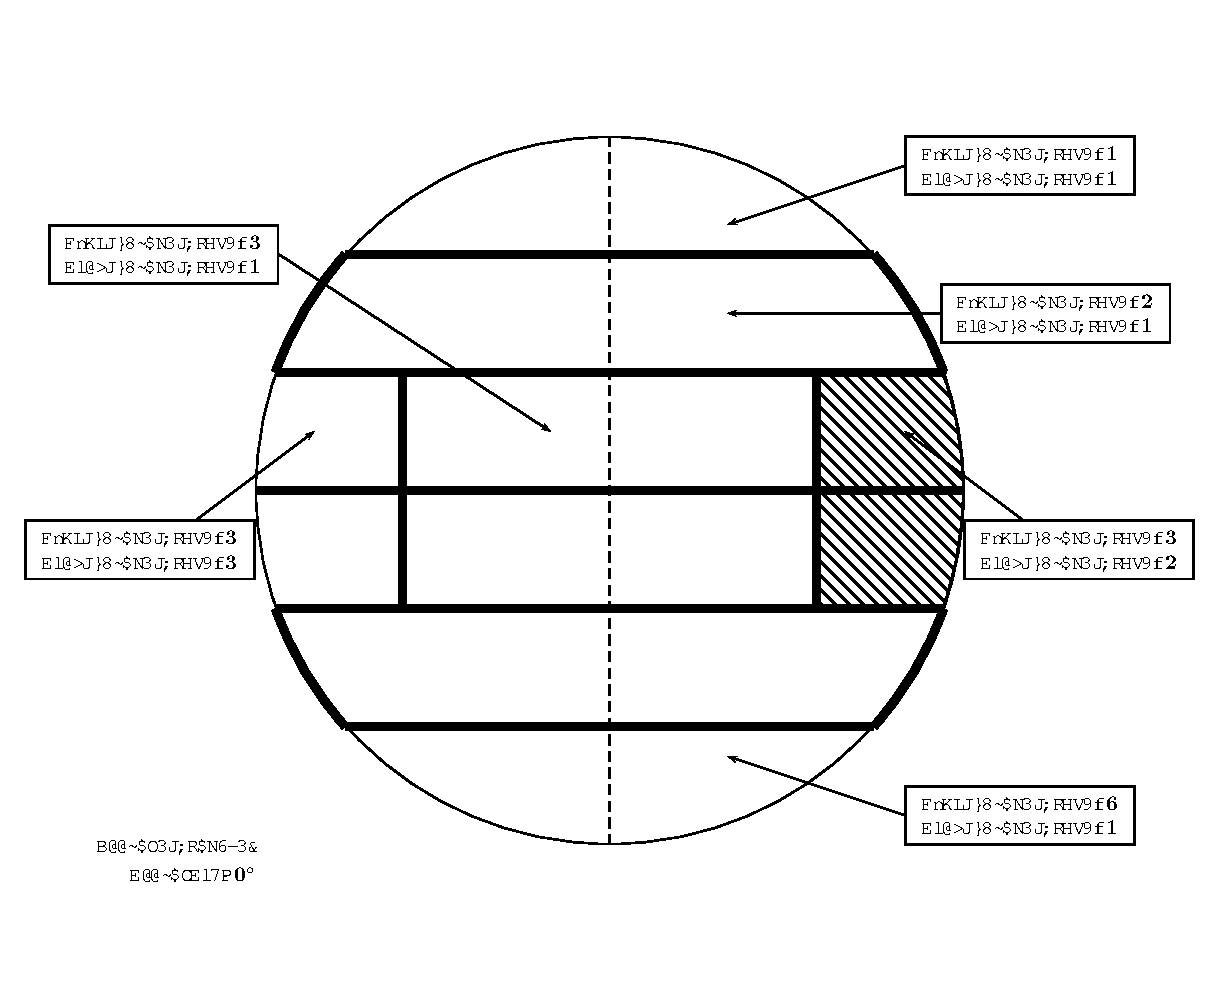
\includegraphics[width=12cm]{rgau_fig.ps}
\end{center}
\caption{適合ガウス格子の例}
\label{rgau_fig}
\end{figure}
Figure \ref{rgau_fig} のように全球を分割する場合を考える(ガウス格子では
緯度の間隔は一定ではないが、ここでは簡単にするため等間隔の場合を
考える)。全球のすべての
格子を格納する場合は、SUBC RGAU に設定する値は 

\noindent
{\tt j = 6}, {\tt j\_start = 1}, {\tt j\_n = 6}, \\
{\tt i(1) = 1}, {\tt i(2) = 2}, {\tt i(3) = 3}, {\tt i(4) = 3}, 
{\tt i(5) = 2}, {\tt i(6) = 1},\\ 
{\tt i\_start(1) = 1}, {\tt i\_start(2) = 1}, {\tt i\_start(3) = 1}, \\
{\tt i\_start(4) = 1}, {\tt i\_start(5) = 1}, {\tt i\_start(6) = 1}, \\
{\tt i\_n(1) = 1}, {\tt i\_n(2) = 2}, {\tt i\_n(3) = 3}, {\tt i\_n(4) = 3}, 
{\tt i\_n(5) = 2}, {\tt i\_n(6) = 1},\\ 
{\tt lat(1) = 75.0}, {\tt lat(2) = 45.0}, {\tt lat(3) = 15.0}, 
{\tt lat(4) = -15.0}, {\tt lat(5) = -45.0}, {\tt lat(6) = -75.0}\\
とする。このとき、データは1次元配列に
\begin{center}
\begin{tabular}{|c|c|c|c|c|c|c|c|c|c|c|c|c|c|} \hline
(1,1) & (1,2) & (2,2) & (1,3) & (2,3) & (3,3) &
(1,4) & (2,4) & (3,4) & (1,5) & (2,5) & (1,6)\\ \hline
\end{tabular} 
\end{center}
のように格納する。

Figure \ref{rgau_fig} の斜線部分のみを格納する場合は\\
{\tt j = 6}, {\tt j\_start=3}, {\tt j\_n = 2}, \\
{\tt i(1) = 1}, {\tt i(2) = 1}, \\
{\tt i\_start(1) = 2}, {\tt i\_start(2) = 2}, \\
{\tt i\_n(1) = 1}, {\tt i\_n(2) = 1}, \\
{\tt lat(1) = 15.0}, {\tt lat(2) = -15.0}, \\
とする。このとき、データは1次元配列に
\begin{center}
\begin{tabular}{|c|c|} \hline
(2,3) & (2,4)\\ \hline
\end{tabular} 
\end{center}
のように格納する。

\section{メルカトル図法 (MR)}

\paragraph{表式}
メルカトル図法 Mercator projection は
世界地図などによく用いられる円筒図法で正角図法でもある。
気象庁では一部の FAX 図や低緯度の台風モデル%
\footnote{
	台風モデルは中緯度ではランベルト正角円錐図法となり、
	事前に投影法が定めがたいため、
	データセット種別名では {\tt \_TYMXXET} などのように {\tt XX} を用いる。
}などで用いられている。

投影の表式は次のようである%
\footnote{
	巷間よく行われる説明では地球中心に光源を置き
	地球に巻きつけた円筒に写る像だといっているが
	あれは子供だましで正角図法にはならない。
	正しくは経線等間隔を仮定して
 	\EqRef{eq:conformal}
	を南北に積分する。
}:
\begin{eqnarray}
 (x - x_0) D_X &=& R (\lambda - \lambda_0)
\\
 (y - y_0) D_Y &=&
 	R \ln\left[\tan\left(\frac{\pi}{4} + \frac{\varphi}{2}\right)\right]
 	-R \ln\left[\tan\left(\frac{\pi}{4} + \frac{\varphi_0}{2}\right)\right]
\\
	&=& R \tanh^{-1}(\sin\varphi)
	- R \tanh^{-1}(\sin\varphi_0)
\\
 R &=& a\cos\varphi_1
\end{eqnarray}
ただしここで \(\tanh^{-1}\) は \(\tanh\) の逆関数であり逆数ではない。

\paragraph{定義ファイル}
この投影を決定するために必要なパラメタは
参照格子点 \(x_0\), \(y_0\),
参照経緯度 \(\lambda_0\), \(\varphi_0\),
格子間隔 \(D_X\), \(D_Y\) (メートル単位, \(D_i\) などと混同しないように)
および標準緯度%
\footnote{
	$D_X$ は標準緯度における東西方向の長さである。
}%
\(\varphi_1\)
であり、定義ファイルに次のように書かれる。
\begin{quote}
\begin{tabular}{lllll}
{\tt distance}	& $D_X$ & $D_Y$ & & \\
{\tt basepoint}	& $x_0$ & $y_0$	& $\lambda_0${\tt E} & $\varphi_0${\tt N} \\
{\tt standard}	& {\tt 0E} & $\varphi_1${\tt 0N} & {\tt 0E} & {\tt 0N} \\
\end{tabular}
\end{quote}

\paragraph{パラメタの許容範囲}
投影法は
\(-90^\circ < \varphi_1 < 90^\circ\),
\(D_X \ne 0\),
\(D_Y \ne 0\)
を要請する。
また NuSDaS インターフェイスによって
\(0 \le |\lambda_0| < 180^\circ\),
が要請される。
理論上何ら悪いことはないのだが、
\(|D_X| < 180\)m
または
\(|D_Y| < 180\)m
という場合は経緯度格子と間違えている可能性が高いので、
エラーではないが警告が表示される。

\section{ポーラーステレオ図法 (PS)}

\paragraph{表式}
ポーラーステレオ図法 polar stereographic projection は
高緯度の天気図や航空向け GPV プロダクトなどに用いられる方位図法で
正角図法でもある。
表式は次のようである。
\begin{eqnarray}
 (x - x_0) D_X &=& R \sin(\lambda-\lambda_1) - R_0 \sin(\lambda_0-\lambda_1)
\\
 (y - y_0) D_Y &=& R \cos(\lambda-\lambda_1) - R_0 \cos(\lambda_0-\lambda_1)
\\
 R &=& a(1 + \sin\varphi_1) \tan \frac{\frac{\pi}{2} - \varphi}{2}
\\
 R_0 &=& a(1 + \sin\varphi_1) \tan \frac{\frac{\pi}{2} - \varphi_0}{2}
\end{eqnarray}
参照点への平行移動や標準緯度 \((\varphi_1)\) による縮尺調整の関係で式が長いが、
要は極からの半径が \(a(1 + \sin\varphi_1)\tan[\frac{1}{2}(\frac{\pi}{2} - \varphi)]\) 
といっているに過ぎない。
南極に光源を置いて北極に接するように置いた平面に映る影が
ステレオ図法だと説明されることが多いが、
ポーラーステレオについては間違っていない%
\footnote{ヒントは円周角の定理}%
。
ここで標準緯度とは、縮尺を変えない円周を与える緯度であり、つまり投影面を置く緯度に他ならない。

\paragraph{定義ファイル}
投影を同定するのに必要なパラメタは
\((x_0, y_0)\),
\((\lambda_0, \varphi_0)\)
および標準緯度 \(\varphi_1\) と標準経度 \(\lambda_1\) であり
定義ファイルに次のように書かれる。
\begin{quote}
\begin{tabular}{lllll}
{\tt distance}	& $D_X$ & $D_Y$ & & \\
{\tt basepoint}	& $x_0$ & $y_0$	& $\lambda_0${\tt E} & $\varphi_0${\tt N} \\
{\tt standard}	& $\lambda_1${\tt E} & $\varphi_1${\tt N} & {\tt 0E} & {\tt 0N} \\
\end{tabular}
\end{quote}
次の例は標準緯度 $60^\circ$N で $140^\circ$E が $y$ 軸になる
ように投影した面の中で
40km 間隔 $83\times 71$ 格子の (65, 53) が ($30^\circ$N, $140^\circ$E) に
来るように配置したものを意味する。
\begin{screen}
\begin{verbatim}
size        83   71
basepoint   65.0   53.0   140.0E  30.0N
distance    40000.0  40000.0
standard    140.0E 60.0N 0.0E 0.0N
\end{verbatim}
\end{screen}

\paragraph{パラメタの許容範囲}
投影法は
\(0 < |\varphi_1| < 90^\circ\),
\(D_X \ne 0\),
\(D_Y \ne 0\)
を要請する。
NuSDaS インターフェイスは
メルカトル図法のチェックに加えて
\(|\lambda_1| \le 180^\circ\)
を要請する。

\section{ランベルト正角円錐図法 (LM)}

\paragraph{表式}
ランベルト正角円錐図法 Lambert conformal conic projection 
(正角割円錐図法 などいろいろに呼ばれる)
はポーラーステレオに比べれば中緯度での縮尺の変動が小さい円錐図法で、
正角図法であることから中緯度の天気図や領域モデルによく用いられる。

\begin{eqnarray}
 (x - x_0) D_X
 &=&
 R\sin[n(\lambda - \lambda_1)]
 - R_0\sin[n(\lambda_0 - \lambda_1)]
 \label{eq:lambert:first}
\\
 (y - y_0) D_Y
 &=&
 R\cos[n(\lambda - \lambda_1)]
 - R_0\cos[n(\lambda_0 - \lambda_1)]
\\
 R
 &=&
 F \tan^{n} \left(\frac{\frac{\pi}{2} - \varphi}{2}\right)
\\
 R_0
 &=&
 F \tan^{n} \left(\frac{\frac{\pi}{2} - \varphi_0}{2}\right)
\\
 F
 &=&
 \frac{a}{n} \cos\varphi_1
 \tan^{-n} \left(\frac{\frac{\pi}{2} - \varphi_1}{2}\right)
 \nonumber
\\
 &=&
 \frac{a}{n} \cos\varphi_2
 \tan^{-n} \left(\frac{\frac{\pi}{2} - \varphi_2}{2}\right)
\\
 n
 &=&
 \frac{ \ln\cos\varphi_1 - \ln\cos\varphi_2 }%
 {
	\ln\tan\left(\frac{\frac{\pi}{2} - \varphi_1}{2}\right)
	- \ln\tan\left(\frac{\frac{\pi}{2} - \varphi_2}{2}\right)
 }
 \label{eq:lambert:last}
\end{eqnarray}

なお、
\(\varphi_1 = \varphi_2\)
の特殊な場合は \EqRef{eq:lambert:last} は
零割る零になってしまうので
計算できず、かわりに極限である
\(
n = \sin\varphi_1
\)
とする。

\paragraph{定義ファイル}
この投影法を同定するために必要なパラメタは
\(x_0, y_0\),
\(\lambda_0, \varphi_0\),
および 標準経度
\(\lambda_1\)
と 2 つの標準緯度
\(\varphi_1, \varphi_2\),
であり、定義ファイルには次のように書かれる ($\lambda_1$ は重出)。
\begin{quote}
\begin{tabular}{lllll}
{\tt distance}	& $D_X$ & $D_Y$ & & \\
{\tt basepoint}	& $x_0$ & $y_0$	& $\lambda_0${\tt E} & $\varphi_0${\tt N} \\
{\tt standard}	& $\lambda_1${\tt E} & $\varphi_1${\tt N} &
	$\lambda_1${\tt E} & $\varphi_2${\tt N} \\
\end{tabular}
\end{quote}

次の例は RSM で用いられているもので、
標準緯度 ($30^\circ$N, $60^\circ$N) として
$140^\circ$E が $y$ 軸となるように投影した
面の中で 20km 間隔 $325\times 257$ 格子の (200, 185) が
($30^\circ$N, $140^\circ$E) に来るように配置したものを意味する。

\begin{screen}
\begin{verbatim}
size        325 257
basepoint   200.  185.  140.0E  30.0N
distance    20000. 20000.
standard    140.0E  30.0N 140.0E  60.0N
\end{verbatim}
\end{screen}

\paragraph{パラメタの許容範囲}
投影法が
\(0 < |\varphi_1| \le |\varphi_2| < 90^\circ\),
\(\varphi_1\varphi_2 > 0\),
\(D_X \ne 0\),
\(D_Y \ne 0\)
を要請する。
NuSDaS インターフェイスは
{\bf ポーラーステレオの条件に加えて}
上のチェックを行う。

\section{斜軸ランベルト図法 (OL)}
\label{sec:proj:OL}

\paragraph{表式}
斜軸ランベルト図法は基本的に上述のランベルト図法の投影中心を北極から
中緯度の適当な地点に移したもので、マップファクターの等しい線が緯線ではなく
経線・緯線と斜めに交わる任意の小円に設定できて、
日本列島のように描画対象が弧状に存在している場合に図全体での
縮尺の差を小さくすることができることに意義がある。
ただし地球の楕円体性の考慮の方式にいろいろあり、
単に斜軸ランベルトというだけでは具体的地図投影写像はひとつには決まらない。

経緯度から地図座標への変換は大きく分けて3段階からなる。
\begin{itemize}
\item
	回転楕円体等角写像
\item
	斜軸回転
\item
	ランベルト正角円錐図法
\end{itemize}

まず回転楕円体等角写像は
回転楕円体上の点\footnote{
	一般に用いられる経緯度は回転楕円体上の経緯度である。
}
\((\lambda, \varphi)\)
を球面上の点
\((\hat{\lambda}, \hat{\varphi})\)
に対応付けるもので、次のようなものである:
\begin{eqnarray}
 \hat{\lambda} &=& c(\lambda - \lambda_E) + \lambda_E
 \label{eq:gauss-aposphere:lon}
\\
 \hat{\varphi} &=&
	2\tan^{-1} \left[
		\tan \frac{\frac{\pi}{2} + \varphi}{2}
		\left(
			\frac{1 - e\sin\varphi}{1 + e\sin\varphi}
		\right)^{\frac{e}{2}}
	\right]^{c}
	- \frac{\pi}{2}
 \label{eq:gauss-aposphere:lat}
\\
 c &=& \sqrt{
   \frac{1 + e^2\cos^4(\varphi_E)}{1 - e^2}
 \label{eq:gauss-aposphere:last}
 }
\end{eqnarray}
ここでパラメタ $e$ は回転楕円体の離心率と呼ばれ
GRS80 系の $0.081819218$ が用いられる。
なお、Snyder \cite{snyder} によれば
\begin{eqnarray}
	\hat{\lambda} &=& \lambda
	\label{eq:snyder-aposphere:lon}
\\
	\hat{\varphi} &=&
	2\tan^{-1} \left[
		\tan \frac{\frac{\pi}{2} + \varphi}{2}
		\left(
			\frac{1 - e\sin\varphi}{1 + e\sin\varphi}
		\right)^{\frac{e}{2}}
	\right]
	- \frac{\pi}{2}
	\label{eq:snyder-aposphere:lat}
\end{eqnarray}
のようにしても等角写像を得ることができて、
もちろんこのほうが2つのパラメタが不要で
簡単だし全球が写像できるメリットもあるのだが
座標値が 10km 単位でずれるので
数値予報標準ライブラリ以外の方法で地図投影している
GIS ソフトウエアの利用にあたっては注意を要する。

次に行われる斜軸回転とは、
正軸球座標における (\(\hat{\lambda}_P, \hat{\varphi}_P\)) を
新座標における北極 (\(\varphi' = \pi/2\)) に対応付け、
正軸球座標における北極を新座標における経度ゼロとするような
新しい球座標 (\(\lambda', \varphi'\)) であり、
次のような式が用いられている。
\begin{eqnarray}
 \varphi' &=& \sin^{-1}\left[
 	\sin\hat{\varphi}_P\sin\hat{\varphi}
 	+ \cos\hat{\varphi}_P\cos\hat{\varphi}
	\cos(\hat{\lambda} - \hat{\lambda}_P)
	\right]
 \label{eq:rotate:lat}
\\
 \lambda' &=& \tan^{-1}\frac{
 	\cos\hat{\varphi}\sin(\hat{\lambda} - \hat{\lambda}_P)
 }{
 	\cos\hat{\varphi}_P\sin\hat{\varphi}
	- \sin\hat{\varphi}_P\cos\hat{\varphi}
	\cos(\hat{\lambda} - \hat{\lambda}_P)
 }
 \label{eq:rotate:lon}
\end{eqnarray}
この変換は地軸に関する経度方向の $\hat{\lambda}_P$ 回転と
東経 90 度軸に関する
\(
 \hat{\theta}_P = \frac{\pi}{2} - \hat{\varphi}_P
\)
だけの回転の合成であるはずだから
\begin{eqnarray*}
 \pmatrix{
  \cos\varphi'\cos{\lambda}' \cr
  \cos\varphi'\sin{\lambda}' \cr
  \sin\varphi' \cr
 }
 &=&
 \pmatrix{
  \cos\hat{\theta}_P & 0 & -\sin\hat{\theta}_P \cr
  0 & 1 & 0 \cr
  \sin\hat{\theta}_P & 0 & \cos\hat{\theta}_P \cr
 }
 \pmatrix{
  \cos\hat{\lambda}_P & \sin\hat{\lambda}_P & 0 \cr
  -\sin\hat{\lambda}_P & \cos\hat{\lambda}_P & 0 \cr
  0 & 0 & 1 \cr
 }
 \pmatrix{
  \cos\hat{\varphi}\cos\hat{\lambda} \cr
  \cos\hat{\varphi}\sin\hat{\lambda} \cr
  \sin\hat{\varphi} \cr
 }
\\
 &=&
 \pmatrix{
  \sin\hat{\varphi}_P \cos\hat{\varphi} \cos(\hat{\lambda} - \hat{\lambda}_P)
  - \cos\hat{\varphi}_P \sin\hat{\varphi}
  \cr
  \cos\hat{\varphi} \sin(\hat{\lambda} - \hat{\lambda}_P)
  \cr
  \cos\hat{\varphi}_P \cos\hat{\varphi} \cos(\hat{\lambda} - \hat{\lambda}_P)
  + \sin\hat{\varphi}_P \sin\hat{\varphi}
  \cr
 }
\end{eqnarray*}
となるが、\EqRef{eq:rotate:lon} の \(\lambda'\) と符号が逆であるから
\(\lambda'\) は西経が正となっていることを意味する。

最後のランベルト正角円錐図法による地図投影は、
式 \ref{eq:lambert:first}--\ref{eq:lambert:last} の
経緯度
\(\lambda', \varphi'\)
に斜軸球面経緯度
\(\lambda', \varphi'\)
をあてはめればよいが、次のようなことに注意されたい。
\begin{itemize}
\item
	パラメタ、特に \(\lambda_1\) は斜軸座標の値である
\item
	気象庁の斜軸ランベルトでは
	極から参照点に向かう軸 (南東向き) を $x$,
	それに右向き直交する軸 (南西向き) を $y$ としているので
	式 \ref{eq:lambert:first}--\ref{eq:lambert:last} の
	$x, y$ を入れ換えたものにあたる
\end{itemize}

\paragraph{定義ファイル}

この投影法を同定するために必要なパラメタは正軸ランベルトのパラメタに加えて
斜軸回転のパラメタ
\(\hat\lambda_P, \hat\varphi_P\),
と楕円体等角写像のパラメタ
\(\lambda_E, \varphi_E\),
であり、定義ファイルには次のように書かれる。
\begin{quote}
\begin{tabular}{lllll}
{\tt distance}	& $D_X$ & $D_Y$ & & \\
{\tt basepoint}	& $x_0$ & $y_0$	& $\lambda_0${\tt E} & $\varphi_0${\tt N} \\
{\tt standard}	& $\lambda_0${\tt E} & $\varphi_1${\tt N} &
	$\lambda_0${\tt E} & $\varphi_2${\tt N} \\
{\tt others} & $\hat\lambda_P${\tt E} & $\hat\varphi_P${\tt N} &
	$\lambda_E${\tt E} & $\varphi_E${\tt N} \\
\end{tabular}
\end{quote}
STANDARD 文にも $\lambda_0$ が書かれておりランベルト投影の標準経度
\(\lambda_1\)
が独立に示されていないが、
気象庁では参照点 \(\lambda_0, \varphi_0\) を楕円体等角写像・斜軸回転
して得る斜軸経度を用いるためである。
%
次の例は 1km 格子である。
%
\begin{screen}
\begin{verbatim}
size        1600 3600
distance    1000 1000
basepoint   1053 1403 35.3572N 138.7306E
standard    45.8183N 138.7306E 50.9429N 138.7306E
others      56.1920N 82.7382E 37.0N 137.0E
\end{verbatim}
\end{screen}

\paragraph{投影法パラメタの由来}

気象庁で用いられている斜軸ランベルト図法は格子間隔と
参照点格子番号を除いて上の定義ファイル例のパラメタを用いているが、これは
国土地理院が 1972 年に発行した
300 万分の 1 「日本とその周辺」図の投影法に由来する。
\(
	\lambda_E = 137^\circ, \varphi_E = 37^\circ
\)
は別にすると
\( \hat\lambda_P = 82^\circ44'17''.4 \),
\( \hat\varphi_P = 56^\circ11'31''.3 \),
\( \varphi_1 = 45^\circ49'06''.0 \),
\( \varphi_2 = 50^\circ56'34''.4 \)
は
大変切りの悪い数値であるが、
導線 (縮尺が最小となる線で斜軸座標の緯線) が
占守島 (\(50^\circ46'\)N, \(156^\circ03'\)E)\footnote{
	占守島は幌筵島
	(32215 SEVERO-KRIL'SK 50:41N, 145:08E) より東だからこの経度は
	明らかに間違っている。
	ちなみに名古屋と台北の経緯度はちょうど 47636 と 46692 に一致する。
}
名古屋 (\(35^\circ10'\)N, \(136^\circ58'\)E),
台北 (\(25^\circ02'\)N, \(121^\circ31'\)E),
を通り、その縮尺が 0.999 となるように決められているという\cite{kanazawa}。
参照点
\(\lambda_0 = 138^\circ43'50''\),
\(\varphi_0 = 35^\circ21'26''\)
はレーダーエコー合成図に由来し、
富士山の経緯度である\cite{makihara}。

当時のことであるから (特に富士山の) 経緯度は
旧日本測地系によるものであるが、
現在でも前節の投影法パラメタを
そのままに地球の形だけ GRS80 系に変更して用いている。
理論上この斜軸座標は 2002 年 4 月 1 日の改正測量法施行時
あるいは地球の形として GRS80 系が採用された NAPS8 の移行時に
400--500m ほどシフトされたことになるが、
それが問題になるプロダクトは今のところ存在しない。

\paragraph{パラメタの許容範囲}
現在のところ正軸ランベルトと同じチェックが行われる。

\section{子午面断面図 (YP)}
\paragraph{定義ファイル}
鉛直22層、南北73格子の例を次に示す。
\begin{screen}
\begin{verbatim}
plane 1
plane1 ZONAL
size 73 22
basepoint 1 1 0E 90N
distance 2.5 2.5
\end{verbatim}
\end{screen}
\paragraph{パラメタの許容範囲}
\(0 < |D_J| < 180^\circ\),
\(|\lambda_0| \le 180^\circ\),
\(|\varphi_0| \le 90^\circ\)
が要請される。

\section{東西断面図 (XP)}

\paragraph{定義ファイル}
鉛直1層、東西360格子の例を次に示す。
\begin{screen}
\begin{verbatim}
size 360 1
basepoint 1 1 0E 0N
distance 1.0 1.0
\end{verbatim}
\end{screen}
\paragraph{パラメタの許容範囲}
\(0 < |D_I| < 180^\circ\),
\(|\lambda_0| \le 180^\circ\),
\(|\varphi_0| \le 90^\circ\)
が要請される。

\section{レーダー画像 (RD)}

\paragraph{定義}
国内二進電文の資料から察して
レーダーサイトを中心とした正距方位図法の投影面上の等間隔格子であると解されるが
投影法諸元を掲げることができるような厳密な定義は調査中である。
\paragraph{定義ファイル}
格子間隔が書かれる。
メンバー毎に違うレーダーサイトを表現する
多メンバーのデータセットにすることが多いので
参照点は書かれないのが普通である。
また、レーダーデータについては通常 \verb|value REPR| が書かれる。
\begin{screen}
\begin{verbatim}
size        200 200
distance    2500 2500
value       REPR
\end{verbatim}
\end{screen}

\paragraph{パラメタの許容範囲}
投影法は
\(D_X \ne 0\),
\(D_Y \ne 0\)
を要請する。
理論上何ら悪いことはないのだが、
\(|D_X| < 180\)m
または
\(|D_Y| < 180\)m
という場合は経緯度格子と間違えている可能性が高いので、
エラーではないが警告が表示される。
また、\DefRef{BASEPOINT} を書いた場合は経緯度が過大だとエラーになる。

\paragraph{注意}
なお、次項で述べる極座標に {\tt RD} を用いている例があるため注意を要する。
このようなデータは $D_X$ に比べて $D_Y$ だけが桁違いに小さい。

\section{レーダー極座標格子 (RT)}

\paragraph{定義}
X ($r$) 軸が距離、Y ($\theta$) 軸が方位角である。
したがって通常 $D_\theta = 360^\circ / N_Y$ である。
方位角の原点は北であると思うがデータ作成元に確認されたい
(将来の版ではこの点を明確化する必要がある)。

\paragraph{定義ファイル}
次のような形式で記述する。

\begin{quote}
\begin{tabular}{lll}
{\tt size} & $N_X$ & $N_Y$ \\
{\tt distance} & $D_r$ & $D_\theta$ \\
\end{tabular}
\end{quote}

具体例を挙げると次のようになる。

\begin{screen}
\begin{verbatim}
size        200  256
distance    1500  1.40625
value       REPR
\end{verbatim}
\end{screen}

\paragraph{パラメタの許容範囲}
投影法は
\(D_r \ne 0\),
\(0 < |D_\theta| < 180^\circ\)
を要請する。
理論上何ら悪いことはないのだが、
\(|D_r| < 180\)m
という場合は経緯度格子と間違えている可能性が高いので、
エラーではないが警告が表示される。


\section{地点 (ST)}
\paragraph{表式}
アメダスデコードについて利用されている。
この格子系のデータについては、
データ要素として経緯度
{\tt LAT},
{\tt LON},
または
{\tt MLAT},
{\tt MLON},
が格納されていなければ、
各格子点の位置についてはデータ作成元に問い合わせるほかない。
\paragraph{定義ファイル}
投影法関連の文 [\DefRef{DISTANCE} 等] は通常省略される。
\paragraph{パラメタの許容範囲}
特段のチェックは行われない。

\section{細分 (SB)}
\paragraph{表式}
検証デコードについて利用されている。
この格子系のデータについては、
データ要素として、細分番号
{\tt SB\_NUM},
が格納されていなければ、
各格子点の位置についてはデータ作成元に問い合わせるほかない。
\paragraph{定義ファイル}
投影法関連の文 [\DefRef{DISTANCE} 等] は通常省略される。
\paragraph{パラメタの許容範囲}
特段のチェックは行われない。

\section{自由格子 (FG)}
\paragraph{表式}
河川に沿った格子について利用されている。
この格子系のデータについては、
各格子点の位置についてはデータ作成元に問い合わせるほかない。
\paragraph{定義ファイル}
投影法関連の文 [\DefRef{DISTANCE} 等] は通常省略される。
\paragraph{パラメタの許容範囲}
特段のチェックは行われない。

\section{その他の格子 (XX)}
\label{sec:proj:XX}

この「座標系」は台風モデルによって用いられている。
台風モデルは台風の中心位置が低緯度のときメルカトル図法、
中緯度のときランベルト正角円錐図法となるので、
事前に種別名を定めておきたい
(あるいは、台風モデルの出力をひとつのデータセットに蓄積したい)
という目的から便宜上 {\tt XX} を用いる。
台風モデルは実行時に \APIRef{nusdas.grid}{nusdas\_grid} を用いて
投影法パラメタを設定している。

このような運用に配慮して、
2次元座標系が {\tt XX} のときは
データファイルを作成しようとするときに行われる投影法パラメタチェックが
抑止される。
そのかわり、ファイルを閉じようとするさいに依然として
投影法が {\tt XX} であれば、
nusdas\_grid を呼び忘れたものとみなしてエラーになる。

\Chapter{3次元座標系と鉛直座標パラメタ}
\label{chap:3dcoord}

\section{気圧座標 (PP)}
気圧$p$ を独立変数にした座標系である。
座標を構成するにあたって必要なパラメータはない。

面名は hPa 単位で数値を6文字の文字列(左詰めで余りには空白を埋め
る)で表す。

\section{エータ座標 (ET)}
$\sigma - p$ 座標とも呼ばれ、下層では地形に沿った$\sigma$座標系、上層で
は水平な $p$ 座標系になっている(Figure \ref{eta_full_half})。

\begin{figure}[h]
\begin{center}
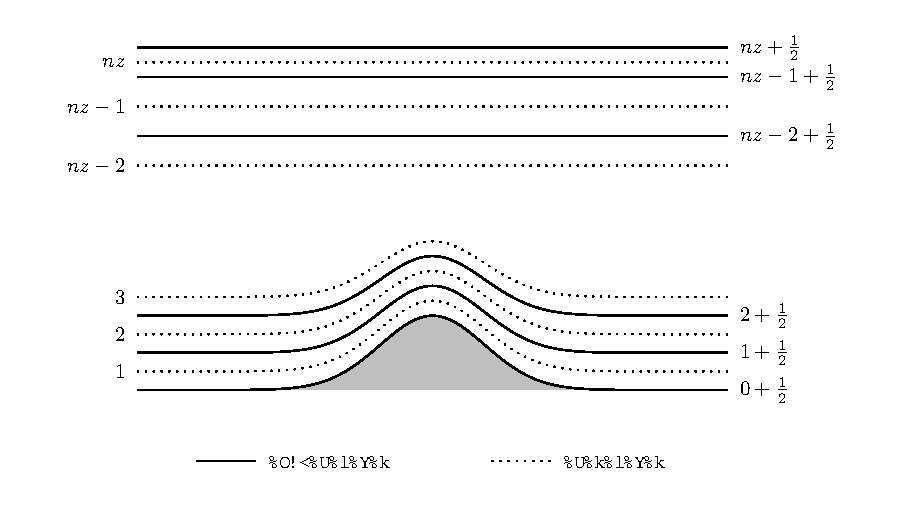
\includegraphics[height=6cm]{eta_full_half.ps}
\end{center}
\caption{エータ座標系の模式図(GSM, RSMなど)。
 地表面はハーフレベルの最下層に一致する。
 この地表面まで含めたときにハーフレベルの層数は鉛直層数(フルレベルの層数)
 より1だけ多いことに注意。そのため、ハーフレベルに対応する値を格納する
 SUBC ETA の$A$, $B$ の要素数が(鉛直層数+1)必要になる。}
\label{eta_full_half}
\end{figure}

各点の気圧は、SUBC ETA レコードに格納されている係数 $A$, $B$, $C$ を用い
て
\[
 p(x, y, z) = B(z)[p_G(x, y, z) - C] + A(z)
\]
と表現される(実際には$C=0$である)。

$A$, $B$ は、ハーフレベルに対応した値が格納されており\footnote{$p$はハー
フレベルに配置されている。}、ハーフレベルの最下層が地表面に一致するよう
になっている。また、ハーフレベルはフルレベルより1層多いので、$A$, $B$ は
鉛直層数(フルレベルの層数) に1を加えた数の配列を確保する必要がある。

データは通常、フルレベルの値が格納され、層名は下からつけた番号を
6文字の文字列(左詰めで余りには空白を埋める)で表す。

\section{シグマ座標 (SG)}
ある一定の気圧を $p_T$、地表面の気圧を $p_G$、各点の気圧を $p$ としたと
き、
\[
 \sigma(x, y, z) = \frac{p(x, y, z) - p_T}{p_G(x, y) - p_T}
\]
で定義された変数を独立変数にする座標系である。

地形に沿った座標系で、地球表面に山があっても、地表面は
$\sigma = 1$ で表される。

各点の気圧は、ETA 座標と同様に、
SUBC SIGM レコードに格納されている係数 $A$, $B$, $C$ を用い
て
\[
 p(x, y, z) = B(z)[p_G(x, y, z) - C] + A(z)
\]
と表現される($A$, $B$, $C$ については、ETA と同じ要素数を持つ配列または
変数)。
$A$が $p_T$ に、$B$ が $\sigma$ に、$C$ が $p_T$ に対応する
\footnote{$p_T$ はスカラーであるが、ETAとデータ構造を同じにするため、
配列である $A$ に格納している。格納の際には、すべての要素に同じ値を格納
するようにする。}。


データは通常、フルレベルの値が格納され、層名は下からつけた番号を
6文字の文字列(左詰めで余りには空白を埋める)で表す。

\section{ハイブリッド気圧座標 (HB)}

用例はない。名前だけ予約されていると解されたい。
鉛直座標パラメタを格納するために
SUBC ETA レコードで対応できるか否かも未定である。

\section{バイブリッド鉛直座標(Z*座標の拡張)(ZS)}
一般に、絶対高度座標 $z$ と変換した座標系の座標 $\zeta$ が
\[
 z = \zeta + z_s f(\zeta)
\]
の関係式に表される座標系である。Z*座標系($\zeta$ を $z^*$と標記する)
\[
 z^* = \frac{z_T(z-z_s)}{H-z_s}
\]
は、
\[
 f(\zeta) = 1-\frac{\zeta}{z_T}
\]
としたものである。
ここで、$z_s$ は地形、$z_T$ はモデルトップである。

運動方程式に中に現れる座標変換に伴うテンソルは
\begin{eqnarray*}
 G^{\frac12} &=& 1 + z_s f'(\zeta) \\
 G^{\frac12}G^{13} &=& -f(\zeta)\frac{\partial z_s}{\partial x} \\
 G^{\frac12}G^{23} &=& -f(\zeta)\frac{\partial z_s}{\partial y}
\end{eqnarray*}
と表現できて、高度$z$やテンソルの算出にはモデル面の高度$\zeta$、
$f(\zeta)$および$f'(\zeta)$ があればよい。

NuSDaS では SUBC ZHYB に、モデル面の高度$\zeta$を
{\tt zrp}(フルレベル)、{\tt zrw}(ハーフレベル)、$f(\zeta)$ を \newline
{\tt vctrans\_p}(フルレベル)、{\tt vctrans\_w}(ハーフレベル)、
$f'(\zeta)$ を{\tt dvtrans\_p}(フルレベル)、{\tt dvtrans\_w}(ハーフレベ
ル)として格納されている。
\section{高度による鉛直座標 (ZZ)}
(地形を考慮しない)高度を鉛直座標にとった座標系である。

\section{温位座標 (TH)}
温位を鉛直座標にとった座標系である。
用例は確立されていないが、温位がケルビン単位の整数であれば単にその値を
\verb|printf("%g")| したものを面名にするのが適当である。

\section{経度 (LO)}

二次元座標系が {\tt YP} の時に用いられる。
実際には経度の値が用いられることはなく、
東西平均 {\tt ZONAL} だけが用いられる。

そうでないときはおとなしく {\tt LL PP} を使ってもらいたい。

\section{緯度 (LA)}

二次元座標系が {\tt XP} の時に用いられるため予約された名前である。
用例はない。

\section{閾値 (TO)}
閾値を面とみなして扱うもので、実際の鉛直座標系ではない。
主に、検証で使用する。

\section{その他の鉛直座標 (XX)}

GRIB 等のデコーダで未知の座標を表現するために予約された名前であり、
積極的に使うべきでない。

 % Chapter 
 \chapter{パッキング}
\label{chap:packing}
\section{一般論}

パッキング (packing) とは、数値データを圧縮保存する技法のひとつで、
線形変換によってデータをビット数の少ない別の型
(たいていは整数) に近似的に変換することによって使用ビット数を減らすものです。
以下の {\tt 1PAC}, {\tt 2PAC}, {\tt 2UPC}, {\tt 4PAC}
がその (本来の) パッキングにあたります (数字がバイト数を表します)。
この圧縮は不可逆で、
データを {\tt nusdas\_write} してから {\tt nusdas\_read} しても
元のデータとは一致しません。

NuSDaS ではパッキングという言葉が少々拡大解釈されていて、
定義ファイルの PACKING 文 \SectionRef{sec:def:PACKING} などによって
パッキングだけでなく、
ランレングス圧縮 {\tt RLEN} などの圧縮 (compression) や
数値型をそのまま保存する方式が選択できるようになっています。


\section{1PAC}

8ビット (1バイト) 符号なし整数で保存するパッキングです。

エンコード (データ列 $y_i$ からファイルに書くべき整数列 $n_i$ を求めるとき)
には次のようにします:
\begin{eqnarray}
b &:=& \min_i(y_i) \\
a &:=& \frac{\max_i(y_i) - \min_i(y_i)}{252} \\
n_i &:=& {\rm floor}\left[\frac{y_i - b}{a} + 0.5\right]
\end{eqnarray}
ここで、${\rm floor}[x]$ は小数部切り捨てです。
式から明らかですが $0 \le n_i \le 252$ となりますので
8 ビット符号なし整数で表現できるわけです。
データ列がすべて同じ値の場合は、$a=1, n_i = 0$ とされます。
ちなみに $a$ の名前は amplitude (振幅), $b$ の名前は
base (ここでは最小値のつもりの和製英語) からきています。

デコード (ファイルから読んだ $a, b, n_i$ からデータを復元するとき) は
\begin{equation}
y_i' := a n_i + b
\end{equation}
として、もとのデータに近い浮動小数点数 $y_i'$ を復元します。

{\tt 1PAC} の読み書きは、
ユーザー配列の型が{\tt I2}, {\tt I4}, {\tt R4}, {\tt R8} でなければなりません。

\section{2PAC}

16ビット (2バイト) {\bf 符号付き}整数で保存するパッキングです。
{\bf これを使ってはいけません。}

エンコードは次のようになっています:
\begin{eqnarray}
b &:=& \frac{\max_i(y_i) + \min_i(y_i)}{2} \\
a &:=& \frac{\max\left[\max_i(y_i) - b, b - \min_i(y_i)\right]}{32765} \\
n_i &:=& {\rm floor}\left[\frac{y_i - b}{a} + 0.5\right]
\end{eqnarray}
デコードの方法は 1PAC と同じです。
かつて $a$ の決め方が悪く $n_i > 32767$ となって
とんでもない値がデコードされるバグがあったのは修正されています。
しかし最小値が再現しないため、積算降水量の差をとると負の降水量が生じる、
といった問題は本質的に解消不能なため、
NAPS8 以降の数値予報ルーチンでは 2PAC の使用は禁止されています。

{\tt 2PAC} の読み書きは、
ユーザー配列の型が{\tt I4}, {\tt R4}, {\tt R8} でなければなりません。

\section{2UPC}
16ビット (2バイト) 符号なし整数で保存するパッキングです。

エンコードは次のようです:
\begin{eqnarray}
b &:=& \min_i(y_i) \\
a &:=& \frac{\max_i(y_i) - \min_i(y_i)}{65532} \\
n_i &:=& {\rm floor}\left[\frac{y_i - b}{a} + 0.5\right]
\end{eqnarray}

{\tt 2UPC} の読み書きは、
ユーザー配列の型が{\tt I4}, {\tt R4}, {\tt R8} でなければなりません。

\section{4PAC}

32ビット (4バイト) 符号つき整数で保存するパッキングです。
あまり使われません。

エンコードは次のようです:
\begin{eqnarray}
b &:=& \frac{\max_i(y_i) + \min_i(y_i)}{2} \\
a &:=& \frac{\max\left[\max_i(y_i) - b, b - \min_i(y_i)\right]}{2147483645} \\
n_i &:=& {\rm floor}\left[\frac{y_i - b}{a} + 0.5\right] \label{eq:2upc:n}
\end{eqnarray}

{\tt 4PAC} の読み書きは、
ユーザー配列の型が{\tt R4} または {\tt R8} でなければなりません。

\section{N1I2}

10倍した値を符号付き2バイト整数に変換してファイルに格納する。

ユーザー配列の型は{\tt R4}, {\tt I2}, {\tt I4} に限られる。

このPACK型の場合は、ユーザー配列の型によって以下のように挙動が異なるので
注意が必要である。
\subsection{ユーザー配列型がR4の場合}
エンコードの際には、ユーザー配列の値を10倍した値を符号付き2バイト整数に
キャストした値をファイルに格納する。
デコードの際には、符号付き2バイト整数 を 10 で除した値を浮動小数点数にキャ
ストしてユーザー配列に格納する。

すなわち、ユーザー配列の値は実際の値でよい。

\subsection{ユーザー配列型がI2, I4の場合}
エンコードの際には、ユーザー配列そのままの値を符号付き2バイト整数にキャスト
した値をファイルに格納する。
デコードの際には、符号付き2バイト整数を符号付き2バイト整数、または符号付
き4バイト整数にキャストしてユーザー配列に格納する。

ユーザー側で、
エンコードの際には10倍を、デコードの際には0.1倍をする必要があるので注意。

\section{RLEN}
非負のデータを圧縮するための
ランレングス符号化法である。1次元に連続したデータがある場合、その値と同
じ値のデータの継続する長さ(ランレングス)を1つのセットとし、セットをつな
げることで1次元に連続したデータを表現する手法である。

圧縮データの中で一つの格子点値が占めるビット数を変えることで、様々な範囲
の(非負の)整数データを圧縮できるが、
 NuSDaS では 8ビットのみをサポートしている。

ユーザー配列の型は
{\tt I1}, {\tt I2}, {\tt I4}, {\tt R4}, {\tt R8}が使えるが、エンコードで
きるデータは符号なし1バイト整数で表現できる範囲である%
\footnote{
厳密には、符号なし1バイト整数の最大値である255を含むデータは圧縮できない。
データの最大値{\tt MAXV}を超えたデータは、値 -- {\tt MAXV}を
その直前の値のランレングスとするが、{\tt MAXV}が255ではランレングスを
表現できないからである。254 ではランレングスとして1だけを表現できるが、
ランレングスが1の場合は圧縮の意味がない。
}。

ランレングスのデータは、ビット数{\tt NBIT}、データの最大値{\tt MAXV}、
データ列から構成される。

データ列を符号なしで{\tt NBIT}ずつ区切って読んだとき、
{\tt MAXV}以下の値は格子点の値とする。{\tt MAXV} を超える値は、ランレン
グスを表すものとする。1セットは、まず値を配置し、もしその値が連続するよ
うであれば後ろにランレングスを付加することによって作られる。{\tt MAXV}
より大きなデータが続く場合はすべてそのセットのランレングスの情報であり、
{\tt MAXV} 以下のデータが現れた時点でそのセットは終了し、この{\tt MAXV}
以下のデータは次のセットの値になる。また、同じ値が連続しない場合は
ランレングスは付加されず、次のセットに移る。

ランレングスは $L = 2^{\tt NBIT} - 1 - {\tt MAXV}$ としたとき、$L$進数に
よって表現している。{\tt MAXV} を超える値が$N$個続いた場合、その値を
$a_n(n = 1, 2, \cdots, N)$(インデックスは出現順)とすると
ランレングス$R$は
\begin{equation}
R=\sum_{n = 1}^{N}\left[L^{(n-1)}\{a_n- ({\tt MAXV + 1})\}\right] + 1
\end{equation}
と求めることができる。

\section{I1}
ユーザー配列を符号なし1バイト整数型にキャストして格納する。

\section{I2}
ユーザー配列を符号つき2バイト整数型にキャストして格納する。

\section{I4}
ユーザー配列を符号つき4バイト整数型にキャストして格納する。

\section{R4}
ユーザー配列を単精度浮動小数点型にキャストして格納する。

\section{R8}
ユーザー配列を倍精度浮動小数点型にキャストして格納する。

\section{2UPJ}

{\tt 2UPC} と同様にデータを 16 ビット符号なし整数で表現した後、
整数列を JPEG2000 圧縮したものをファイルに格納する。
レポジトリでは 2009-11-04 に追加された機能。

{\tt 2UPJ} の読み書きは、ユーザー配列の型が {\tt I4},
{\tt R4}, {\tt R8} に限られる
({\tt N\_NC} によるレコード内容直接読み取りは 2010-04-21 に追加された)。

\section{2UPP}

{\tt 2UPC} と同様にデータを 16 ビット符号なし整数で表現した後、整数列を
複合差分圧縮 (GRIB2 DRT5.3 に類似) したものをファイルに格納する。
まず、{\tt 2UPC}の式\ref{eq:2upc:n}で得られたバイト列$n_k$に対して以下の$p_k$を作成する。
\begin{equation}
  p_k = \left\{ \begin{array}{ll}
    \mathrm{mod}\left(n_k + 32768, \, 
      65536\right) & (k = 0, 1) \,, \\
    \mathrm{mod}\left(n_{k} - 2n_{k-1} + n_{k-2} + 32768, \,
      65536\right) & (k \geq 2) \,,
  \end{array} \right.
\end{equation}

NuSDaSの複合差分圧縮では$p_k$を32格子単位の群ごとに保存する。
格子数$N$のときの群数は
\begin{equation}
N_G = (N - 1) / 32 + 1,
\end{equation}
で得られる\footnote{$N=0$のとき$N_G=1$となるので注意}。
ただし最後の群に所属する格子の数は32未満になる可能性がある。
$p_k$を群$i$の$j$番目のデータとして
\begin{equation}
P_{ij} \equiv p_k \quad \left(i=k/32,\,j=\mathrm{mod}\left(k,32\right) \right),
\end{equation}
と割り当てた後、以下の処理を行う。
\begin{eqnarray}
R_i &=& \min_j \left(P_{ij}\right) \,, \\
D_{ij} &=& P_{ij} - R_i \,, \\
W_i &=& \mathrm{bits}\left(\max_j\left(D_{ij}\right)\right) - 1 \,.
\end{eqnarray}

$\mathrm{bits}(m)$は整数$m$のbit幅を求める関数で例えば
$\mathrm{bits}(5) = 3$となる。ただし
$\mathrm{bits}(0) \equiv 1$として扱う。$R_i$の取りうる値は
$0$から$65535$、$W_i$は$0$から$15$の値をとりうる。
また$D_{ij}$のすべての値は必ず$(W_i+1)$bit幅で表現できる。
このようにして求めた$R_i$, $W_i$をそれぞれ2バイト幅、4bit幅で
\ref{table.fmt.data.2upp}に格納する。複合差分圧縮されたデータ本体$D_{ij}$は
\ref{table.fmt.data.2upp}の圧縮データの位置に$(W_i + 1)$bit幅で格納する

{\tt 2UPP} の読み書きは、ユーザー配列の型が {\tt I4},
{\tt R4}, {\tt R8} に限られる。

 % Chapter 
 \Chapter{仕様の変更点}

\section{pnusdas}

リトルエンディアン機で動作するようになりました。

\section{NuSDaS 1.1}
\subsection{ファイルにおける「レコード長」の変更}
ファイルの各レコードの先頭、末尾各4バイトに書き込まれているレコード長を
そのレコード長そのものの8バイトを除いた長さにするようにしました
(NuSDaS10では、その8バイトを含めた長さになっていました)。これによっ
て、ファイルがFortran 順編成ファイルになりました。
\subsection{ファイル長の上限が2GBから4GBへ}
従来は、{\tt INDX}レコードを符号付き4byte整数としていたため、ファイルの大きさ
が符号付き4byte整数の表現範囲の上限である約 2GB に制限されていましたが、これ
を符号なし4byte整数として解釈するように変更して、約 4GB までに制限が緩和され
ました。

\subsection{同一TYPEのNRDが複数ある時のNRD探索}
同一のTYPE1,2,3 の NuSDaS Root Directory(NRD) が複数ある場合、
従来は最初に見つかったNRDからデータ取得ができなければ、失敗として
エラーを返していましたが、データ取得が成功するまでNRDの探索を継続
するようにしました。
\subsection{ランレングス圧縮において1byte整数のユーザーデータをサポート}
従来はランレングス圧縮のユーザーデータの型は4byte整数だけをサポー
トしていましたが、1byte整数もサポートするようにしました。
\subsection{高速化}
ファイル書き込みの際にバッファリングを行うことにより、ファイル書き
込みの高速化を図りました。

%%%% 確かに多数の関数が追加されたけど、広く公開していないので、
%%%% 言及しなくてもよいかも  tabito
%多数の関数が追加されました。

\section{NuSDaS 1.2}

SUBC RGAU, SUBC ZHYB, SUBC DELT 記録のアクセス関数が追加されました。

\section{NuSDaS 1.3}
\label{changes13}

\subsection{Fortran での定数 NULL の廃止}

あまりに実装が難しいため、
Fortran インターフェイスでの定数 {\bf NULL} が廃止されました。
\\* nusdas\_parameter\_change()
で設定したパラメタを既定値に戻すには、明示的に既定値を設定するか、新設の
\\* nusdas\_parameter\_reset()
を用いてください。

\subsection{ファイル名生成}

定義ファイルの filename 文にスラッシュと
{\tt \_basetime} などの置換指定を使うと互換性がなくなります。
ディレクトリは path 文に記述するようにしてください。

\subsection{CNTL 記録の大きさ}

NuSDaS 1.3 で作られる CNTL 記録に書かれる対象時刻のリストは、
定義ファイルの予報時間リスト (VALIDTIME1 文) と
基準時刻から導かれる対象時刻すべてとなります。

従来は定義ファイルの設定により、対象時刻のリストが1対象時刻だけとなる
場合がありました。

\subsection{コーデック}\label{chgs-codec}

nusdas\_read や nusdas\_write などで与えるユーザ配列の型と
パッキング方式の組合せはなんでもよいわけではないのですが、
許される組合せが増えました。

特に、{\tt RLEN} パッキングで不適切なユーザ配列型
({\bf N\_I2}, {\bf N\_R4}, {\bf N\_R8})
を与えた場合に不定動作となるバグに対処しました。

一方、{\bf N\_NC} 機能は 2012年9月19日時点では {\tt 2UPC} パッキング
および {\tt 2UPJ} パッキングだけについて実装されています。
(NuSDaS 1.4 からは {\tt 2UPP} も追加)

\subsection{SUBC 記録}

SUBC 記録を書き込んでいない状況で
nusdas\_subc\_tdif(),
nusdas\_subc\_srf(),
nusdas\_subc\_delt() (NuSDaS 1.2 のみ)
で読出しを行った場合、
従来は異常が通知されずすべてゼロの値が返されますが、
エラーコード $-2$ で異常終了するようにしました。

データファイルが存在しない状況で
SUBC 記録を書き出すと従来はエラーコード $-51$ で異常終了していましたが、
正常に書き出せるようになりました。

性能上の理由から
NUSD--SUBC, INFO, END 記録の書き出しはファイルを閉じるときまで遅延されます。
そこで SUBC 記録を出力したプログラムがファイルを閉じることなく
異常終了すると当該 SUBC 記録の内容が読出せなくなります
(従来版では読出せることがある)。

\subsection{INFO 記録}

リトルエンディアン機で定義ファイルによって INFO 記録を作成すると
群名が反転 (例: ${\tt VSRF} \to {\tt FRSV}$) するバグが対処されています。

INFO 記録を読み出すときバッファ長が不足していると
従来はバッファ長だけ読出して正常終了していましたが
エラーコード $-3$ で異常終了するようにしました。

データファイルが存在しない状況で
INFO 記録を書き出すと従来はエラーコード $-51$ で異常終了していましたが、
正常に書き出せるようになりました。

\section{NuSDaS 1.4}
\label{changes14}

NAPS9 運用開始後 2020年1月までの主な変更は次のとおりです。
チケット番号 (\#717) 、リビジョン番号 (r4369) などは開発管理サーバ Redmine の番号です。

\paragraph{\#717, r4369}
入出力モジュール aio, mmap, ibmshmat が廃止されました。

\paragraph{r4376}
実行時オプション GSVB が新設されました。

\paragraph{\#720, r4380}
ES 対応が入りました。

\paragraph{\#745, r4386}
OpenMP に対応しました。

\paragraph{\#752, r4407}
リトルエンディアン機でのバグ対応。
負値を I2 または I4 型のパッキングで保存して R4 に読み出すと、
あたかも符号なし整数であったかのような大きな値が読み出されていました。

\paragraph{\#765, r4413}
SUBCを上書きするとENDレコードが壊れる問題に対処しました。

\paragraph{\#771, r4420}
複合差分圧縮 packing = 2UPP を導入しました。

\paragraph{\#770, r4432}
NAPS インストールツールを再び動作するようにしました。

\paragraph{\#848}
複合差分圧縮でOpenMPに対応しました。

\paragraph{\#934}
計算誤差によって欠損値が設定していない格子に欠損値が格納される不具合を修正しました。

\paragraph{\#1037}
2UPP展開サブルーチンを追加しました。

\paragraph{\#1162}
intelコンパイラでjpeg2000利用時に配列侵害を起こす不具合を修正しました。

\paragraph{\#1242}
SUBC INFOレコードで初期化せず利用する変数を初期化するよう変更しました。

\paragraph{\#1248}
矩形ガウス格子の出力でリトルエンディアン機に対応しました。

\paragraph{\#1643}
2UPP,2UPJ 書き込み時のメモリリークが起きないよう対応しました。

\paragraph{\#1678}
[122]PAC, 2UP[CPJ] で 負の0による不一致がでないよう修正しました。

\paragraph{\#1684}
ISS(GPFS)のテープアクセス判定を追加しました。

\paragraph{\#1764}
NuSDaS\_inq\_data で対象ファイルが存在しない場合に N\_DATA\_EXIST の戻り値が不定とならないよう修正しました。

\paragraph{\#1788}
close時にfsyncを実行する処理を追加しました。

\paragraph{\#1803}
デバッグ時にタイムスタンプを出力しないオプションNTMSを追加しました。

\paragraph{\#1856}
動的ライブラリとして利用しやすいよう、リンク切れ修正しました。

\paragraph{\#1876}
N\_ND を新規実装しました。

\paragraph{\#1881}
NUSDレコードとENDレコードのレコード数が不正な値になる不具合を修正しました。

\paragraph{\#2015}
lustre flush を利用してLustreの末尾欠落問題に対応しました。

\paragraph{\#2045}
末尾欠落に該当したレコード読み込みの戻り値が正常に読み込みの値となるバグを修正しました。

\paragraph{\#2080}
NTMSオプションの名称をGNTSに修正しました。




 % Chapter 
 \sloppy
 \Chapter{範囲指定型 API (廃止予定)}
\label{api2}

\section{概要}

NuSDaS 内部では、対象時刻および面は点ではなく
範囲として表現できるようになっています
(GRIB から変換ができるように配慮したのでしょう)。
対象時刻は整数 2 つで期間の始点と終点を表わし、
面は 6 文字の名前 2 つで上端と下端の高度を表わすことができます。
これらはそれぞれ「対象時刻1」「対象時刻2」「面1」「面2」と呼ばれます。

対象時刻2や面2が指定されない「範囲でないデータ」は、
対象時刻2が値 $1$%
\footnote{通算分 1 は欠損をあらわします。
1801 年 1 月 1 日 00:01Z と区別つきませんが、おそらく問題にはならないでしょう}
で面2と面1が同じものとして表現されています。

対象時刻または面名に範囲を用いるデータセットを読み書きするために、
本章で説明する API が用意されています。
これらは関数名の末尾に `2' がつくので区別されます。
しかし、実際には積算・平均の時間範囲は範囲指定ではなく、
SUBC TDIF レコード {}[\TabRef{table.fmt.subc.tdif}] によって表現されます。

対象時刻2や面2を用いた範囲指定は Pandora では利用できなくなりました。
本章で説明される関数・サブルーチンも、
将来のライブラリ再設計時には削除される予定ですので、
開発環境のアプリケーションに用例があった場合は
速やかに `2なし' API に移行するように努めてください。

\section{Fortran API}
\label{fapi2}

\renewcommand{\APILabel}[1]{\label{fapi:#1}}

\subsection{NUSDAS\_CUT2: 領域限定のデータ読取 }
\APILabel{nusdas.cut2}

\Prototype
\begin{quote}
CALL {\bf NUSDAS\_CUT2}({\it type1}, {\it type2}, {\it type3}, {\it basetime}, {\it member}, {\it validtime1}, {\it validtime2}, {\it plane1}, {\it plane2}, {\it element}, {\it udata}, {\it utype}, {\it usize}, {\it ixstart}, {\it ixfinal}, {\it iystart}, {\it iyfinal}, {\it result})
\end{quote}

\begin{tabular}{l|rllp{16em}}
\hline
\ArgName & \ArgType & \ArrayDim & I/O & \ArgRole \\
\hline
{\it type1} & CHARACTER(8) &  & IN &  種別1  \\
{\it type2} & CHARACTER(4) &  & IN &  種別2  \\
{\it type3} & CHARACTER(4) &  & IN &  種別3  \\
{\it basetime} & INTEGER(4) &  & IN &  基準時刻(通算分)  \\
{\it member} & CHARACTER(4) &  & IN &  メンバー名  \\
{\it validtime1} & INTEGER(4) &  & IN &  対象時刻1  \\
{\it validtime2} & INTEGER(4) &  & IN &  対象時刻2  \\
{\it plane1} & CHARACTER(6) &  & IN &  面1  \\
{\it plane2} & CHARACTER(6) &  & IN &  面2  \\
{\it element} & CHARACTER(6) &  & IN &  要素名  \\
{\it udata} & \AnyType & \AnySize & OUT &  データ格納配列  \\
{\it utype} & CHARACTER(2) &  & IN &  データ格納配列の型  \\
{\it usize} & INTEGER(4) &  & IN &  データ格納配列の要素数  \\
{\it ixstart} & INTEGER(4) &  & IN &  $x$ 方向格子番号下限  \\
{\it ixfinal} & INTEGER(4) &  & IN &  $x$ 方向格子番号上限  \\
{\it iystart} & INTEGER(4) &  & IN &  $y$ 方向格子番号下限  \\
{\it iyfinal} & INTEGER(4) &  & IN &  $y$ 方向格子番号上限  \\
{\it result} & INTEGER(4) &  & OUT & \ResultCode \\
\hline
\end{tabular}

\subsection{NUSDAS\_CUT2\_RAW: 領域限定の DATA 記録直接読取 }
\APILabel{nusdas.cut2.raw}

\Prototype
\begin{quote}
CALL {\bf NUSDAS\_CUT2\_RAW}({\it type1}, {\it type2}, {\it type3}, {\it basetime}, {\it member}, {\it validtime1}, {\it validtime2}, {\it plane1}, {\it plane2}, {\it element}, {\it udata}, {\it usize}, {\it ixstart}, {\it ixfinal}, {\it iystart}, {\it iyfinal}, {\it result})
\end{quote}

\begin{tabular}{l|rllp{16em}}
\hline
\ArgName & \ArgType & \ArrayDim & I/O & \ArgRole \\
\hline
{\it type1} & CHARACTER(8) &  & IN &  種別1  \\
{\it type2} & CHARACTER(4) &  & IN &  種別2  \\
{\it type3} & CHARACTER(4) &  & IN &  種別3  \\
{\it basetime} & INTEGER(4) &  & IN &  基準時刻(通算分)  \\
{\it member} & CHARACTER(4) &  & IN &  メンバー名  \\
{\it validtime1} & INTEGER(4) &  & IN &  対象時刻1(通算分)  \\
{\it validtime2} & INTEGER(4) &  & IN &  対象時刻2(通算分)  \\
{\it plane1} & CHARACTER(6) &  & IN &  面1  \\
{\it plane2} & CHARACTER(6) &  & IN &  面2  \\
{\it element} & CHARACTER(6) &  & IN &  要素名  \\
{\it udata} & \AnyType & \AnySize & OUT &  データ格納先配列  \\
{\it usize} & INTEGER(4) &  & IN &  データ格納先配列のバイト数  \\
{\it ixstart} & INTEGER(4) &  & IN &  $x$ 方向格子番号下限  \\
{\it ixfinal} & INTEGER(4) &  & IN &  $x$ 方向格子番号上限  \\
{\it iystart} & INTEGER(4) &  & IN &  $y$ 方向格子番号下限  \\
{\it iyfinal} & INTEGER(4) &  & IN &  $y$ 方向格子番号上限  \\
{\it result} & INTEGER(4) &  & OUT & \ResultCode \\
\hline
\end{tabular}
\paragraph{\FuncDesc}nusdas\_cut\_raw の範囲指定版。nusdas\_cut を参照。

\subsection{NUSDAS\_GRID2: 格子情報へのアクセス }
\APILabel{nusdas.grid2}

\Prototype
\begin{quote}
CALL {\bf NUSDAS\_GRID2}({\it type1}, {\it type2}, {\it type3}, {\it basetime}, {\it member}, {\it validtime1}, {\it validtime2}, {\it proj}, {\it gridsize}, {\it gridinfo}, {\it value}, {\it getput}, {\it result})
\end{quote}

\begin{tabular}{l|rllp{16em}}
\hline
\ArgName & \ArgType & \ArrayDim & I/O & \ArgRole \\
\hline
{\it type1} & CHARACTER(8) &  & IN &  種別1  \\
{\it type2} & CHARACTER(4) &  & IN &  種別2  \\
{\it type3} & CHARACTER(4) &  & IN &  種別3  \\
{\it basetime} & INTEGER(4) &  & IN &  基準時刻(通算分)  \\
{\it member} & CHARACTER(4) &  & IN &  メンバー名  \\
{\it validtime1} & INTEGER(4) &  & IN &  対象時刻1(通算分)  \\
{\it validtime2} & INTEGER(4) &  & IN &  対象時刻2(通算分)  \\
{\it proj} & CHARACTER(4) &  & I/O &  投影法3字略号  \\
{\it gridsize} & INTEGER(4) & 2 & I/O &  格子数  \\
{\it gridinfo} & REAL(4) & 14 & I/O &  投影法緒元  \\
{\it value} & CHARACTER(4) &  & I/O &  格子点値が周囲の場を代表する方法  \\
{\it getput} & CHARACTER(3) &  & IN &  入出力指示 ({\it "GET}" または {\it "PUT}")  \\
{\it result} & INTEGER(4) &  & OUT & \ResultCode \\
\hline
\end{tabular}

\subsection{NUSDAS\_INFO2: INFO 記録へのアクセス }
\APILabel{nusdas.info2}

\Prototype
\begin{quote}
CALL {\bf NUSDAS\_INFO2}({\it type1}, {\it type2}, {\it type3}, {\it basetime}, {\it member}, {\it validtime1}, {\it validtime2}, {\it group}, {\it info}, {\it bytesize}, {\it getput}, {\it result})
\end{quote}

\begin{tabular}{l|rllp{16em}}
\hline
\ArgName & \ArgType & \ArrayDim & I/O & \ArgRole \\
\hline
{\it type1} & CHARACTER(8) &  & IN &  種別1  \\
{\it type2} & CHARACTER(4) &  & IN &  種別2  \\
{\it type3} & CHARACTER(4) &  & IN &  種別3  \\
{\it basetime} & INTEGER(4) &  & IN &  基準時刻(通算分)  \\
{\it member} & CHARACTER(4) &  & IN &  メンバー名  \\
{\it validtime1} & INTEGER(4) &  & IN &  対象時刻1(通算分)  \\
{\it validtime2} & INTEGER(4) &  & IN &  対象時刻2(通算分)  \\
{\it group} & CHARACTER(4) &  & IN &  群名  \\
{\it info} & CHARACTER & \AnySize & I/O &  INFO 記録内容  \\
{\it bytesize} & INTEGER(4) &  & IN &  INFO 記録のバイト数  \\
{\it getput} & CHARACTER(3) &  & IN &  入出力指示 ({\it "GET}" または {\it "PUT}")  \\
{\it result} & INTEGER(4) &  & OUT & \ResultCode \\
\hline
\end{tabular}

\subsection{NUSDAS\_INQ\_CNTL2: データファイルの諸元問合せ }
\APILabel{nusdas.inq.cntl2}

\Prototype
\begin{quote}
CALL {\bf NUSDAS\_INQ\_CNTL2}({\it type1}, {\it type2}, {\it type3}, {\it basetime}, {\it member}, {\it validtime1}, {\it validtime2}, {\it param}, {\it data}, {\it datasize}, {\it result})
\end{quote}

\begin{tabular}{l|rllp{16em}}
\hline
\ArgName & \ArgType & \ArrayDim & I/O & \ArgRole \\
\hline
{\it type1} & CHARACTER(8) &  & IN &  種別1  \\
{\it type2} & CHARACTER(4) &  & IN &  種別2  \\
{\it type3} & CHARACTER(4) &  & IN &  種別3  \\
{\it basetime} & INTEGER(4) &  & IN &  基準時刻(通算分)  \\
{\it member} & CHARACTER(4) &  & IN &  メンバー名  \\
{\it validtime1} & INTEGER(4) &  & IN &  対象時刻1(通算分)  \\
{\it validtime2} & INTEGER(4) &  & IN &  対象時刻2(通算分)  \\
{\it param} & INTEGER(4) &  & IN &  問合せ項目コード  \\
{\it data} & \AnyType & \AnySize & OUT &  問合せ結果配列  \\
{\it datasize} & INTEGER(4) &  & IN &  問合せ結果配列の要素数  \\
{\it result} & INTEGER(4) &  & OUT & \ResultCode \\
\hline
\end{tabular}

\subsection{NUSDAS\_INQ\_DATA2: データ記録の諸元問合せ }
\APILabel{nusdas.inq.data2}

\Prototype
\begin{quote}
CALL {\bf NUSDAS\_INQ\_DATA2}({\it type1}, {\it type2}, {\it type3}, {\it basetime}, {\it member}, {\it validtime1}, {\it validtime2}, {\it plane1}, {\it plane2}, {\it element}, {\it item}, {\it data}, {\it nelems}, {\it result})
\end{quote}

\begin{tabular}{l|rllp{16em}}
\hline
\ArgName & \ArgType & \ArrayDim & I/O & \ArgRole \\
\hline
{\it type1} & CHARACTER(8) &  & IN &  種別1  \\
{\it type2} & CHARACTER(4) &  & IN &  種別2  \\
{\it type3} & CHARACTER(4) &  & IN &  種別3  \\
{\it basetime} & INTEGER(4) &  & IN &  基準時刻(通算分)  \\
{\it member} & CHARACTER(4) &  & IN &  メンバー名  \\
{\it validtime1} & INTEGER(4) &  & IN &  対象時刻1(通算分)  \\
{\it validtime2} & INTEGER(4) &  & IN &  対象時刻2(通算分)  \\
{\it plane1} & CHARACTER(6) &  & IN &  面1  \\
{\it plane2} & CHARACTER(6) &  & IN &  面2  \\
{\it element} & CHARACTER(6) &  & IN &  要素名  \\
{\it item} & INTEGER(4) &  & IN &  問合せ項目コード  \\
{\it data} & \AnyType & \AnySize & OUT &  結果格納配列  \\
{\it nelems} & INTEGER(4) &  & IN &  結果格納配列要素数  \\
{\it result} & INTEGER(4) &  & OUT & \ResultCode \\
\hline
\end{tabular}

\input{fapi_nusdas_onefile_close2}
\subsection{NUSDAS\_READ2: データ記録の読取}
\APILabel{nusdas.read2}

\Prototype
\begin{quote}
CALL {\bf NUSDAS\_READ2}({\it utype1}, {\it utype2}, {\it utype3}, {\it basetime}, {\it member}, {\it validtime1}, {\it validtime2}, {\it plane1}, {\it plane2}, {\it element}, {\it data}, {\it fmt}, {\it size}, {\it result})
\end{quote}

\begin{tabular}{l|rllp{16em}}
\hline
\ArgName & \ArgType & \ArrayDim & I/O & \ArgRole \\
\hline
{\it utype1} & CHARACTER(8) &  & IN &  種別1  \\
{\it utype2} & CHARACTER(4) &  & IN &  種別2  \\
{\it utype3} & CHARACTER(4) &  & IN &  種別3  \\
{\it basetime} & INTEGER(4) &  & IN &  基準時刻(通算分)  \\
{\it member} & CHARACTER(4) &  & IN &  メンバー  \\
{\it validtime1} & INTEGER(4) &  & IN &  対象時刻1(通算分)  \\
{\it validtime2} & INTEGER(4) &  & IN &  対象時刻2(通算分)  \\
{\it plane1} & CHARACTER(6) &  & IN &  面の名前1  \\
{\it plane2} & CHARACTER(6) &  & IN &  面の名前2  \\
{\it element} & CHARACTER(6) &  & IN &  要素名  \\
{\it data} & \AnyType & \AnySize & OUT &  結果格納配列  \\
{\it fmt} & CHARACTER(2) &  & IN &  結果格納配列の型  \\
{\it size} & INTEGER(4) &  & IN &  結果格納配列の要素数  \\
{\it result} & INTEGER(4) &  & OUT & \ResultCode \\
\hline
\end{tabular}

\input{fapi_nusdas_subc_delt2}
\input{fapi_nusdas_subc_eta2}
\subsection{NUSDAS\_SUBC\_ETA\_INQ\_NZ2: SUBC 記録の鉛直層数問合せ }
\APILabel{nusdas.subc.eta.inq.nz2}

\Prototype
\begin{quote}
CALL {\bf NUSDAS\_SUBC\_ETA\_INQ\_NZ2}({\it type1}, {\it type2}, {\it type3}, {\it basetime}, {\it member}, {\it validtime1}, {\it validtime2}, {\it group}, {\it n\_levels}, {\it result})
\end{quote}

\begin{tabular}{l|rllp{16em}}
\hline
\ArgName & \ArgType & \ArrayDim & I/O & \ArgRole \\
\hline
{\it type1} & CHARACTER(8) &  & IN &  種別1  \\
{\it type2} & CHARACTER(4) &  & IN &  種別2  \\
{\it type3} & CHARACTER(4) &  & IN &  種別3  \\
{\it basetime} & INTEGER(4) &  & IN &  基準時刻(通算分)  \\
{\it member} & CHARACTER(4) &  & IN &  メンバー名  \\
{\it validtime1} & INTEGER(4) &  & IN &  対象時刻1(通算分)  \\
{\it validtime2} & INTEGER(4) &  & IN &  対象時刻2(通算分)  \\
{\it group} & CHARACTER(4) &  & IN &  群名  \\
{\it n\_levels} & INTEGER(4) &  & OUT &  鉛直層数  \\
{\it result} & INTEGER(4) &  & OUT & \ResultCode \\
\hline
\end{tabular}

\subsection{NUSDAS\_SUBC\_RGAU2: SUBC RGAU へのアクセス }
\APILabel{nusdas.subc.rgau2}

\Prototype
\begin{quote}
CALL {\bf NUSDAS\_SUBC\_RGAU2}({\it type1}, {\it type2}, {\it type3}, {\it basetime}, {\it member}, {\it validtime1}, {\it validtime2}, {\it j}, {\it j\_start}, {\it j\_n}, {\it i}, {\it i\_start}, {\it i\_n}, {\it lat}, {\it getput}, {\it result})
\end{quote}

\begin{tabular}{l|rllp{16em}}
\hline
\ArgName & \ArgType & \ArrayDim & I/O & \ArgRole \\
\hline
{\it type1} & CHARACTER(8) &  & IN &  種別1  \\
{\it type2} & CHARACTER(4) &  & IN &  種別2  \\
{\it type3} & CHARACTER(4) &  & IN &  種別3  \\
{\it basetime} & INTEGER(4) &  & IN &  基準時刻(通算分)  \\
{\it member} & CHARACTER(4) &  & IN &  メンバー名  \\
{\it validtime1} & INTEGER(4) &  & IN &  対象時刻1(通算分)  \\
{\it validtime2} & INTEGER(4) &  & IN &  対象時刻2(通算分)  \\
{\it j} & INTEGER(4) &  & I/O &  全球の南北分割数  \\
{\it j\_start} & INTEGER(4) &  & I/O &  データの最北格子の番号(1始まり)  \\
{\it j\_n} & INTEGER(4) &  & I/O &  データの南北格子数  \\
{\it i} & INTEGER(4) & \AnySize & I/O &  全球の東西格子数  \\
{\it i\_start} & INTEGER(4) & \AnySize & I/O &  データの最西格子の番号(1始まり)  \\
{\it i\_n} & INTEGER(4) & \AnySize & I/O &  データの東西格子数  \\
{\it lat} & REAL(4) & \AnySize & I/O &  緯度  \\
{\it getput} & CHARACTER(3) &  & IN &  入出力指示 ({\it "GET}" または {\it "PUT}")  \\
{\it result} & INTEGER(4) &  & OUT & \ResultCode \\
\hline
\end{tabular}

\subsection{NUSDAS\_SUBC\_RGAU\_INQ\_JN2: SUBC RGAU 記録の大きさを問合せ }
\APILabel{nusdas.subc.rgau.inq.jn2}

\Prototype
\begin{quote}
CALL {\bf NUSDAS\_SUBC\_RGAU\_INQ\_JN2}({\it type1}, {\it type2}, {\it type3}, {\it basetime}, {\it member}, {\it validtime1}, {\it validtime2}, {\it j\_n}, {\it result})
\end{quote}

\begin{tabular}{l|rllp{16em}}
\hline
\ArgName & \ArgType & \ArrayDim & I/O & \ArgRole \\
\hline
{\it type1} & CHARACTER(8) &  & IN &  種別1  \\
{\it type2} & CHARACTER(4) &  & IN &  種別2  \\
{\it type3} & CHARACTER(4) &  & IN &  種別3  \\
{\it basetime} & INTEGER(4) &  & IN &  基準時刻(通算分)  \\
{\it member} & CHARACTER(4) &  & IN &  メンバー名  \\
{\it validtime1} & INTEGER(4) &  & IN &  対象時刻1(通算分)  \\
{\it validtime2} & INTEGER(4) &  & IN &  対象時刻2(通算分)  \\
{\it j\_n} & INTEGER(4) &  & OUT &  南北格子数  \\
{\it result} & INTEGER(4) &  & OUT & \ResultCode \\
\hline
\end{tabular}

\subsection{NUSDAS\_SUBC\_SIGM2: SUBC SIGM へのアクセス }
\APILabel{nusdas.subc.sigm2}

\Prototype
\begin{quote}
CALL {\bf NUSDAS\_SUBC\_SIGM2}({\it type1}, {\it type2}, {\it type3}, {\it basetime}, {\it member}, {\it validtime1}, {\it validtime2}, {\it n\_levels}, {\it a}, {\it b}, {\it c}, {\it getput}, {\it result})
\end{quote}

\begin{tabular}{l|rllp{16em}}
\hline
\ArgName & \ArgType & \ArrayDim & I/O & \ArgRole \\
\hline
{\it type1} & CHARACTER(8) &  & IN &  種別1  \\
{\it type2} & CHARACTER(4) &  & IN &  種別2  \\
{\it type3} & CHARACTER(4) &  & IN &  種別3  \\
{\it basetime} & INTEGER(4) &  & IN &  基準時刻(通算分)  \\
{\it member} & CHARACTER(4) &  & IN &  メンバー名  \\
{\it validtime1} & INTEGER(4) &  & IN &  対象時刻1(通算分)  \\
{\it validtime2} & INTEGER(4) &  & IN &  対象時刻2(通算分)  \\
{\it n\_levels} & INTEGER(4) &  & I/O &  鉛直層数  \\
{\it a} & REAL(4) & \AnySize & I/O &  係数 a  \\
{\it b} & REAL(4) & \AnySize & I/O &  係数 b  \\
{\it c} & REAL(4) &  & I/O &  係数 c  \\
{\it getput} & CHARACTER(3) &  & IN &  入出力指示 ({\it "GET}" または {\it "PUT}")  \\
{\it result} & INTEGER(4) &  & OUT & \ResultCode \\
\hline
\end{tabular}

\subsection{NUSDAS\_SUBC\_SRF2: 降短系 SUBC へのアクセス }
\APILabel{nusdas.subc.srf2}

\Prototype
\begin{quote}
CALL {\bf NUSDAS\_SUBC\_SRF2}({\it type1}, {\it type2}, {\it type3}, {\it basetime}, {\it member}, {\it validtime1}, {\it validtime2}, {\it plane1}, {\it plane2}, {\it element}, {\it group}, {\it data}, {\it getput}, {\it result})
\end{quote}

\begin{tabular}{l|rllp{16em}}
\hline
\ArgName & \ArgType & \ArrayDim & I/O & \ArgRole \\
\hline
{\it type1} & CHARACTER(8) &  & IN &  種別1  \\
{\it type2} & CHARACTER(4) &  & IN &  種別2  \\
{\it type3} & CHARACTER(4) &  & IN &  種別3  \\
{\it basetime} & INTEGER(4) &  & IN &  基準時刻(通算分)  \\
{\it member} & CHARACTER(4) &  & IN &  メンバー名  \\
{\it validtime1} & INTEGER(4) &  & IN &  対象時刻1(通算分)  \\
{\it validtime2} & INTEGER(4) &  & IN &  対象時刻2(通算分)  \\
{\it plane1} & CHARACTER(6) &  & IN &  面1  \\
{\it plane2} & CHARACTER(6) &  & IN &  面2  \\
{\it element} & CHARACTER(6) &  & IN &  要素名  \\
{\it group} & CHARACTER(4) &  & IN &  群名  \\
{\it data} & INTEGER(4) &  & I/O &  データ配列  \\
{\it getput} & CHARACTER(3) &  & IN &  入出力指示 ({\it "GET}" または {\it "PUT}")  \\
{\it result} & INTEGER(4) &  & OUT & \ResultCode \\
\hline
\end{tabular}

\input{fapi_nusdas_subc_tdif2}
\subsection{NUSDAS\_SUBC\_ZHYB2: SUBC ZHYB へのアクセス }
\APILabel{nusdas.subc.zhyb2}

\Prototype
\begin{quote}
CALL {\bf NUSDAS\_SUBC\_ZHYB2}({\it type1}, {\it type2}, {\it type3}, {\it basetime}, {\it member}, {\it validtime1}, {\it validtime2}, {\it nz}, {\it ptrf}, {\it presrf}, {\it zrp}, {\it zrw}, {\it vctrans\_p}, {\it vctrans\_w}, {\it dvtrans\_p}, {\it dvtrans\_w}, {\it getput}, {\it result})
\end{quote}

\begin{tabular}{l|rllp{16em}}
\hline
\ArgName & \ArgType & \ArrayDim & I/O & \ArgRole \\
\hline
{\it type1} & CHARACTER(8) &  & IN &  種別1  \\
{\it type2} & CHARACTER(4) &  & IN &  種別2  \\
{\it type3} & CHARACTER(4) &  & IN &  種別3  \\
{\it basetime} & INTEGER(4) &  & IN &  基準時刻(通算分)  \\
{\it member} & CHARACTER(4) &  & IN &  メンバー名  \\
{\it validtime1} & INTEGER(4) &  & IN &  対象時刻1(通算分)  \\
{\it validtime2} & INTEGER(4) &  & IN &  対象時刻2(通算分)  \\
{\it nz} & INTEGER(4) &  & I/O &  鉛直層数  \\
{\it ptrf} & REAL(4) &  & I/O &  温位の参照値  \\
{\it presrf} & REAL(4) &  & I/O &  気圧の参照値  \\
{\it zrp} & REAL(4) & \AnySize & I/O &  モデル面高度 (フルレベル)  \\
{\it zrw} & REAL(4) & \AnySize & I/O &  モデル面高度 (ハーフレベル)  \\
{\it vctrans\_p} & REAL(4) & \AnySize & I/O &  座標変換関数 (フルレベル)  \\
{\it vctrans\_w} & REAL(4) & \AnySize & I/O &  座標変換関数 (ハーフレベル)  \\
{\it dvtrans\_p} & REAL(4) & \AnySize & I/O &  座標変換関数の鉛直微分 (フルレベル)  \\
{\it dvtrans\_w} & REAL(4) & \AnySize & I/O &  座標変換関数の鉛直微分 (ハーフレベル)  \\
{\it getput} & CHARACTER(3) &  & IN &  入出力指示 ({\it "GET}" または {\it "PUT}")  \\
{\it result} & INTEGER(4) &  & OUT & \ResultCode \\
\hline
\end{tabular}

\subsection{NUSDAS\_WRITE2: データ記録の書出}
\APILabel{nusdas.write2}

\Prototype
\begin{quote}
CALL {\bf NUSDAS\_WRITE2}({\it utype1}, {\it utype2}, {\it utype3}, {\it basetime}, {\it member}, {\it validtime1}, {\it validtime2}, {\it plane1}, {\it plane2}, {\it element}, {\it data}, {\it fmt}, {\it nelems}, {\it result})
\end{quote}

\begin{tabular}{l|rllp{16em}}
\hline
\ArgName & \ArgType & \ArrayDim & I/O & \ArgRole \\
\hline
{\it utype1} & CHARACTER(8) &  & IN &  種別1  \\
{\it utype2} & CHARACTER(4) &  & IN &  種別2  \\
{\it utype3} & CHARACTER(4) &  & IN &  種別3  \\
{\it basetime} & INTEGER(4) &  & IN &  基準時刻(通算分)  \\
{\it member} & CHARACTER(4) &  & IN &  メンバー名  \\
{\it validtime1} & INTEGER(4) &  & IN &  対象時刻1(通算分)  \\
{\it validtime2} & INTEGER(4) &  & IN &  対象時刻2(通算分)  \\
{\it plane1} & CHARACTER(6) &  & IN &  面の名前1  \\
{\it plane2} & CHARACTER(6) &  & IN &  面の名前2  \\
{\it element} & CHARACTER(6) &  & IN &  要素名  \\
{\it data} & \AnyType & \AnySize & IN &  データを与える配列  \\
{\it fmt} & CHARACTER(2) &  & IN &  data の型  \\
{\it nelems} & INTEGER(4) &  & IN &  data の要素数  \\
{\it result} & INTEGER(4) &  & OUT & \ResultCode \\
\hline
\end{tabular}


\section{C API}
\label{capi2}

\renewcommand{\APILabel}[1]{\label{capi:#1}}

\subsection{nusdas\_cut2: 領域限定のデータ読取 }
\APILabel{nusdas.cut2}

\Prototype
\begin{quote}
N\_SI4 {\bf nusdas\_cut2}(const char {\it type1}[8], const char {\it type2}[4], const char {\it type3}[4], const N\_SI4 $\ast${\it basetime}, const char {\it member}[4], const N\_SI4 $\ast${\it validtime1}, const N\_SI4 $\ast${\it validtime2}, const char {\it plane1}[6], const char {\it plane2}[6], const char {\it element}[6], void $\ast${\it udata}, const char {\it utype}[2], const N\_SI4 $\ast${\it usize}, const N\_SI4 $\ast${\it ixstart}, const N\_SI4 $\ast${\it ixfinal}, const N\_SI4 $\ast${\it iystart}, const N\_SI4 $\ast${\it iyfinal});
\end{quote}

\begin{tabular}{l|rp{20em}}
\hline
\ArgName & \ArgType & \ArgRole \\
\hline
{\it type1} & const char [8] &  種別1  \\
{\it type2} & const char [4] &  種別2  \\
{\it type3} & const char [4] &  種別3  \\
{\it basetime} & const N\_SI4 $\ast$ &  基準時刻(通算分)  \\
{\it member} & const char [4] &  メンバー名  \\
{\it validtime1} & const N\_SI4 $\ast$ &  対象時刻1  \\
{\it validtime2} & const N\_SI4 $\ast$ &  対象時刻2  \\
{\it plane1} & const char [6] &  面1  \\
{\it plane2} & const char [6] &  面2  \\
{\it element} & const char [6] &  要素名  \\
{\it udata} & void $\ast$ &  データ格納配列  \\
{\it utype} & const char [2] &  データ格納配列の型  \\
{\it usize} & const N\_SI4 $\ast$ &  データ格納配列の要素数  \\
{\it ixstart} & const N\_SI4 $\ast$ &  $x$ 方向格子番号下限  \\
{\it ixfinal} & const N\_SI4 $\ast$ &  $x$ 方向格子番号上限  \\
{\it iystart} & const N\_SI4 $\ast$ &  $y$ 方向格子番号下限  \\
{\it iyfinal} & const N\_SI4 $\ast$ &  $y$ 方向格子番号上限  \\
\hline
\end{tabular}

\subsection{nusdas\_cut2\_raw: 領域限定の DATA 記録直接読取 }
\APILabel{nusdas.cut2.raw}

\Prototype
\begin{quote}
N\_SI4 {\bf nusdas\_cut2\_raw}(const char {\it type1}[8], const char {\it type2}[4], const char {\it type3}[4], const N\_SI4 $\ast${\it basetime}, const char {\it member}[4], const N\_SI4 $\ast${\it validtime1}, const N\_SI4 $\ast${\it validtime2}, const char {\it plane1}[6], const char {\it plane2}[6], const char {\it element}[6], void $\ast${\it udata}, const N\_SI4 $\ast${\it usize}, const N\_SI4 $\ast${\it ixstart}, const N\_SI4 $\ast${\it ixfinal}, const N\_SI4 $\ast${\it iystart}, const N\_SI4 $\ast${\it iyfinal});
\end{quote}

\begin{tabular}{l|rp{20em}}
\hline
\ArgName & \ArgType & \ArgRole \\
\hline
{\it type1} & const char [8] &  種別1  \\
{\it type2} & const char [4] &  種別2  \\
{\it type3} & const char [4] &  種別3  \\
{\it basetime} & const N\_SI4 $\ast$ &  基準時刻(通算分)  \\
{\it member} & const char [4] &  メンバー名  \\
{\it validtime1} & const N\_SI4 $\ast$ &  対象時刻1(通算分)  \\
{\it validtime2} & const N\_SI4 $\ast$ &  対象時刻2(通算分)  \\
{\it plane1} & const char [6] &  面1  \\
{\it plane2} & const char [6] &  面2  \\
{\it element} & const char [6] &  要素名  \\
{\it udata} & void $\ast$ &  データ格納先配列  \\
{\it usize} & const N\_SI4 $\ast$ &  データ格納先配列のバイト数  \\
{\it ixstart} & const N\_SI4 $\ast$ &  $x$ 方向格子番号下限  \\
{\it ixfinal} & const N\_SI4 $\ast$ &  $x$ 方向格子番号上限  \\
{\it iystart} & const N\_SI4 $\ast$ &  $y$ 方向格子番号下限  \\
{\it iyfinal} & const N\_SI4 $\ast$ &  $y$ 方向格子番号上限  \\
\hline
\end{tabular}
\paragraph{\FuncDesc}nusdas\_cut\_raw の範囲指定版。nusdas\_cut を参照。

\subsection{nusdas\_grid2: 格子情報へのアクセス }
\APILabel{nusdas.grid2}

\Prototype
\begin{quote}
N\_SI4 {\bf nusdas\_grid2}(const char {\it type1}[8], const char {\it type2}[4], const char {\it type3}[4], const N\_SI4 $\ast${\it basetime}, const char {\it member}[4], const N\_SI4 $\ast${\it validtime1}, const N\_SI4 $\ast${\it validtime2}, char {\it proj}[4], N\_SI4 {\it gridsize}[2], float {\it gridinfo}[14], char {\it value}[4], const char {\it getput}[3]);
\end{quote}

\begin{tabular}{l|rp{20em}}
\hline
\ArgName & \ArgType & \ArgRole \\
\hline
{\it type1} & const char [8] &  種別1  \\
{\it type2} & const char [4] &  種別2  \\
{\it type3} & const char [4] &  種別3  \\
{\it basetime} & const N\_SI4 $\ast$ &  基準時刻(通算分)  \\
{\it member} & const char [4] &  メンバー名  \\
{\it validtime1} & const N\_SI4 $\ast$ &  対象時刻1(通算分)  \\
{\it validtime2} & const N\_SI4 $\ast$ &  対象時刻2(通算分)  \\
{\it proj} & char [4] &  投影法3字略号  \\
{\it gridsize} & N\_SI4 [2] &  格子数  \\
{\it gridinfo} & float [14] &  投影法緒元  \\
{\it value} & char [4] &  格子点値が周囲の場を代表する方法  \\
{\it getput} & const char [3] &  入出力指示 ({\it "GET}" または {\it "PUT}")  \\
\hline
\end{tabular}

\subsection{nusdas\_info2: INFO 記録へのアクセス }
\APILabel{nusdas.info2}

\Prototype
\begin{quote}
N\_SI4 {\bf nusdas\_info2}(const char {\it type1}[8], const char {\it type2}[4], const char {\it type3}[4], const N\_SI4 $\ast${\it basetime}, const char {\it member}[4], const N\_SI4 $\ast${\it validtime1}, const N\_SI4 $\ast${\it validtime2}, const char {\it group}[4], char {\it info}[\,], const N\_SI4 $\ast${\it bytesize}, const char {\it getput}[3]);
\end{quote}

\begin{tabular}{l|rp{20em}}
\hline
\ArgName & \ArgType & \ArgRole \\
\hline
{\it type1} & const char [8] &  種別1  \\
{\it type2} & const char [4] &  種別2  \\
{\it type3} & const char [4] &  種別3  \\
{\it basetime} & const N\_SI4 $\ast$ &  基準時刻(通算分)  \\
{\it member} & const char [4] &  メンバー名  \\
{\it validtime1} & const N\_SI4 $\ast$ &  対象時刻1(通算分)  \\
{\it validtime2} & const N\_SI4 $\ast$ &  対象時刻2(通算分)  \\
{\it group} & const char [4] &  群名  \\
{\it info} & char [\,] &  INFO 記録内容  \\
{\it bytesize} & const N\_SI4 $\ast$ &  INFO 記録のバイト数  \\
{\it getput} & const char [3] &  入出力指示 ({\it "GET}" または {\it "PUT}")  \\
\hline
\end{tabular}

\subsection{nusdas\_inq\_cntl2: データファイルの諸元問合せ }
\APILabel{nusdas.inq.cntl2}

\Prototype
\begin{quote}
N\_SI4 {\bf nusdas\_inq\_cntl2}(const char {\it type1}[8], const char {\it type2}[4], const char {\it type3}[4], const N\_SI4 $\ast${\it basetime}, const char {\it member}[4], const N\_SI4 $\ast${\it validtime1}, const N\_SI4 $\ast${\it validtime2}, N\_SI4 {\it param}, void $\ast${\it data}, const N\_SI4 $\ast${\it datasize});
\end{quote}

\begin{tabular}{l|rp{20em}}
\hline
\ArgName & \ArgType & \ArgRole \\
\hline
{\it type1} & const char [8] &  種別1  \\
{\it type2} & const char [4] &  種別2  \\
{\it type3} & const char [4] &  種別3  \\
{\it basetime} & const N\_SI4 $\ast$ &  基準時刻(通算分)  \\
{\it member} & const char [4] &  メンバー名  \\
{\it validtime1} & const N\_SI4 $\ast$ &  対象時刻1(通算分)  \\
{\it validtime2} & const N\_SI4 $\ast$ &  対象時刻2(通算分)  \\
{\it param} & N\_SI4 &  問合せ項目コード  \\
{\it data} & void $\ast$ &  問合せ結果配列  \\
{\it datasize} & const N\_SI4 $\ast$ &  問合せ結果配列の要素数  \\
\hline
\end{tabular}

\subsection{nusdas\_inq\_data2: データ記録の諸元問合せ }
\APILabel{nusdas.inq.data2}

\Prototype
\begin{quote}
N\_SI4 {\bf nusdas\_inq\_data2}(const char {\it type1}[8], const char {\it type2}[4], const char {\it type3}[4], const N\_SI4 $\ast${\it basetime}, const char {\it member}[4], const N\_SI4 $\ast${\it validtime1}, const N\_SI4 $\ast${\it validtime2}, const char {\it plane1}[6], const char {\it plane2}[6], const char {\it element}[6], N\_SI4 {\it item}, void $\ast${\it data}, const N\_SI4 $\ast${\it nelems});
\end{quote}

\begin{tabular}{l|rp{20em}}
\hline
\ArgName & \ArgType & \ArgRole \\
\hline
{\it type1} & const char [8] &  種別1  \\
{\it type2} & const char [4] &  種別2  \\
{\it type3} & const char [4] &  種別3  \\
{\it basetime} & const N\_SI4 $\ast$ &  基準時刻(通算分)  \\
{\it member} & const char [4] &  メンバー名  \\
{\it validtime1} & const N\_SI4 $\ast$ &  対象時刻1(通算分)  \\
{\it validtime2} & const N\_SI4 $\ast$ &  対象時刻2(通算分)  \\
{\it plane1} & const char [6] &  面1  \\
{\it plane2} & const char [6] &  面2  \\
{\it element} & const char [6] &  要素名  \\
{\it item} & N\_SI4 &  問合せ項目コード  \\
{\it data} & void $\ast$ &  結果格納配列  \\
{\it nelems} & const N\_SI4 $\ast$ &  結果格納配列要素数  \\
\hline
\end{tabular}

\subsection{nusdas\_onefile\_close2: ひとつのファイルを閉じる}
\APILabel{nusdas.onefile.close2}

\Prototype
\begin{quote}
N\_SI4 {\bf nusdas\_onefile\_close2}(const char {\it type1}[8], const char {\it type2}[4], const char {\it type3}[4], const N\_SI4 $\ast${\it basetime}, const char {\it member}[4], const N\_SI4 $\ast${\it validtime1}, const N\_SI4 $\ast${\it validtime2});
\end{quote}

\begin{tabular}{l|rp{20em}}
\hline
\ArgName & \ArgType & \ArgRole \\
\hline
{\it type1} & const char [8] &  種別1  \\
{\it type2} & const char [4] &  種別2  \\
{\it type3} & const char [4] &  種別3  \\
{\it basetime} & const N\_SI4 $\ast$ &  基準時刻(通算分)  \\
{\it member} & const char [4] &  メンバー名  \\
{\it validtime1} & const N\_SI4 $\ast$ &  対象時刻1(通算分)  \\
{\it validtime2} & const N\_SI4 $\ast$ &  対象時刻2(通算分)  \\
\hline
\end{tabular}

\subsection{nusdas\_read2: データ記録の読取}
\APILabel{nusdas.read2}

\Prototype
\begin{quote}
N\_SI4 {\bf nusdas\_read2}(const char {\it utype1}[8], const char {\it utype2}[4], const char {\it utype3}[4], const N\_SI4 $\ast${\it basetime}, const char {\it member}[4], const N\_SI4 $\ast${\it validtime1}, const N\_SI4 $\ast${\it validtime2}, const char {\it plane1}[6], const char {\it plane2}[6], const char {\it element}[6], void $\ast${\it data}, const char {\it fmt}[2], const N\_SI4 $\ast${\it size});
\end{quote}

\begin{tabular}{l|rp{20em}}
\hline
\ArgName & \ArgType & \ArgRole \\
\hline
{\it utype1} & const char [8] &  種別1  \\
{\it utype2} & const char [4] &  種別2  \\
{\it utype3} & const char [4] &  種別3  \\
{\it basetime} & const N\_SI4 $\ast$ &  基準時刻(通算分)  \\
{\it member} & const char [4] &  メンバー  \\
{\it validtime1} & const N\_SI4 $\ast$ &  対象時刻1(通算分)  \\
{\it validtime2} & const N\_SI4 $\ast$ &  対象時刻2(通算分)  \\
{\it plane1} & const char [6] &  面の名前1  \\
{\it plane2} & const char [6] &  面の名前2  \\
{\it element} & const char [6] &  要素名  \\
{\it data} & void $\ast$ &  結果格納配列  \\
{\it fmt} & const char [2] &  結果格納配列の型  \\
{\it size} & const N\_SI4 $\ast$ &  結果格納配列の要素数  \\
\hline
\end{tabular}

\subsection{nusdas\_subc\_delt2: SUBC DELT へのアクセス }
\APILabel{nusdas.subc.delt2}

\Prototype
\begin{quote}
N\_SI4 {\bf nusdas\_subc\_delt2}(const char {\it type1}[8], const char {\it type2}[4], const char {\it type3}[4], const N\_SI4 $\ast${\it basetime}, const char {\it member}[4], const N\_SI4 $\ast${\it validtime1}, const N\_SI4 $\ast${\it validtime2}, float $\ast${\it delt}, const char {\it getput}[3]);
\end{quote}

\begin{tabular}{l|rp{20em}}
\hline
\ArgName & \ArgType & \ArgRole \\
\hline
{\it type1} & const char [8] &  種別1  \\
{\it type2} & const char [4] &  種別2  \\
{\it type3} & const char [4] &  種別3  \\
{\it basetime} & const N\_SI4 $\ast$ &  基準時刻(通算分)  \\
{\it member} & const char [4] &  メンバー名  \\
{\it validtime1} & const N\_SI4 $\ast$ &  対象時刻1(通算分)  \\
{\it validtime2} & const N\_SI4 $\ast$ &  対象時刻2(通算分)  \\
{\it delt} & float $\ast$ &  DELT 数値へのポインタ  \\
{\it getput} & const char [3] &  入出力指示 ({\it "GET}" または {\it "PUT}")  \\
\hline
\end{tabular}

\subsection{nusdas\_subc\_eta2: SUBC ETA へのアクセス }
\APILabel{nusdas.subc.eta2}

\Prototype
\begin{quote}
N\_SI4 {\bf nusdas\_subc\_eta2}(const char {\it type1}[8], const char {\it type2}[4], const char {\it type3}[4], const N\_SI4 $\ast${\it basetime}, const char {\it member}[4], const N\_SI4 $\ast${\it validtime1}, const N\_SI4 $\ast${\it validtime2}, N\_SI4 $\ast${\it n\_levels}, float {\it a}[\,], float {\it b}[\,], float $\ast${\it c}, const char {\it getput}[3]);
\end{quote}

\begin{tabular}{l|rp{20em}}
\hline
\ArgName & \ArgType & \ArgRole \\
\hline
{\it type1} & const char [8] &  種別1  \\
{\it type2} & const char [4] &  種別2  \\
{\it type3} & const char [4] &  種別3  \\
{\it basetime} & const N\_SI4 $\ast$ &  基準時刻(通算分)  \\
{\it member} & const char [4] &  メンバー名  \\
{\it validtime1} & const N\_SI4 $\ast$ &  対象時刻1(通算分)  \\
{\it validtime2} & const N\_SI4 $\ast$ &  対象時刻2(通算分)  \\
{\it n\_levels} & N\_SI4 $\ast$ &  鉛直層数  \\
{\it a} & float [\,] &  係数 a  \\
{\it b} & float [\,] &  係数 b  \\
{\it c} & float $\ast$ &  係数 c  \\
{\it getput} & const char [3] &  入出力指示 ({\it "GET}" または {\it "PUT}")  \\
\hline
\end{tabular}

\subsection{nusdas\_subc\_eta\_inq\_nz2: SUBC 記録の鉛直層数問合せ }
\APILabel{nusdas.subc.eta.inq.nz2}

\Prototype
\begin{quote}
N\_SI4 {\bf nusdas\_subc\_eta\_inq\_nz2}(const char {\it type1}[8], const char {\it type2}[4], const char {\it type3}[4], const N\_SI4 $\ast${\it basetime}, const char {\it member}[4], const N\_SI4 $\ast${\it validtime1}, const N\_SI4 $\ast${\it validtime2}, const char {\it group}[4], N\_SI4 $\ast${\it n\_levels});
\end{quote}

\begin{tabular}{l|rp{20em}}
\hline
\ArgName & \ArgType & \ArgRole \\
\hline
{\it type1} & const char [8] &  種別1  \\
{\it type2} & const char [4] &  種別2  \\
{\it type3} & const char [4] &  種別3  \\
{\it basetime} & const N\_SI4 $\ast$ &  基準時刻(通算分)  \\
{\it member} & const char [4] &  メンバー名  \\
{\it validtime1} & const N\_SI4 $\ast$ &  対象時刻1(通算分)  \\
{\it validtime2} & const N\_SI4 $\ast$ &  対象時刻2(通算分)  \\
{\it group} & const char [4] &  群名  \\
{\it n\_levels} & N\_SI4 $\ast$ &  鉛直層数  \\
\hline
\end{tabular}

\subsection{nusdas\_subc\_rgau2: SUBC RGAU へのアクセス }
\APILabel{nusdas.subc.rgau2}

\Prototype
\begin{quote}
N\_SI4 {\bf nusdas\_subc\_rgau2}(const char {\it type1}[8], const char {\it type2}[4], const char {\it type3}[4], const N\_SI4 $\ast${\it basetime}, const char {\it member}[4], const N\_SI4 $\ast${\it validtime1}, const N\_SI4 $\ast${\it validtime2}, N\_SI4 $\ast${\it j}, N\_SI4 $\ast${\it j\_start}, N\_SI4 $\ast${\it j\_n}, N\_SI4 {\it i}[\,], N\_SI4 {\it i\_start}[\,], N\_SI4 {\it i\_n}[\,], float {\it lat}[\,], const char {\it getput}[3]);
\end{quote}

\begin{tabular}{l|rp{20em}}
\hline
\ArgName & \ArgType & \ArgRole \\
\hline
{\it type1} & const char [8] &  種別1  \\
{\it type2} & const char [4] &  種別2  \\
{\it type3} & const char [4] &  種別3  \\
{\it basetime} & const N\_SI4 $\ast$ &  基準時刻(通算分)  \\
{\it member} & const char [4] &  メンバー名  \\
{\it validtime1} & const N\_SI4 $\ast$ &  対象時刻1(通算分)  \\
{\it validtime2} & const N\_SI4 $\ast$ &  対象時刻2(通算分)  \\
{\it j} & N\_SI4 $\ast$ &  全球の南北分割数  \\
{\it j\_start} & N\_SI4 $\ast$ &  データの最北格子の番号(1始まり)  \\
{\it j\_n} & N\_SI4 $\ast$ &  データの南北格子数  \\
{\it i} & N\_SI4 [\,] &  全球の東西格子数  \\
{\it i\_start} & N\_SI4 [\,] &  データの最西格子の番号(1始まり)  \\
{\it i\_n} & N\_SI4 [\,] &  データの東西格子数  \\
{\it lat} & float [\,] &  緯度  \\
{\it getput} & const char [3] &  入出力指示 ({\it "GET}" または {\it "PUT}")  \\
\hline
\end{tabular}

\subsection{nusdas\_subc\_rgau\_inq\_jn2: SUBC RGAU 記録の大きさを問合せ }
\APILabel{nusdas.subc.rgau.inq.jn2}

\Prototype
\begin{quote}
N\_SI4 {\bf nusdas\_subc\_rgau\_inq\_jn2}(const char {\it type1}[8], const char {\it type2}[4], const char {\it type3}[4], const N\_SI4 $\ast${\it basetime}, const char {\it member}[4], const N\_SI4 $\ast${\it validtime1}, const N\_SI4 $\ast${\it validtime2}, N\_SI4 $\ast${\it j\_n});
\end{quote}

\begin{tabular}{l|rp{20em}}
\hline
\ArgName & \ArgType & \ArgRole \\
\hline
{\it type1} & const char [8] &  種別1  \\
{\it type2} & const char [4] &  種別2  \\
{\it type3} & const char [4] &  種別3  \\
{\it basetime} & const N\_SI4 $\ast$ &  基準時刻(通算分)  \\
{\it member} & const char [4] &  メンバー名  \\
{\it validtime1} & const N\_SI4 $\ast$ &  対象時刻1(通算分)  \\
{\it validtime2} & const N\_SI4 $\ast$ &  対象時刻2(通算分)  \\
{\it j\_n} & N\_SI4 $\ast$ &  南北格子数  \\
\hline
\end{tabular}

\input{capi_nusdas_subc_sigm2}
\subsection{nusdas\_subc\_srf2: 降短系 SUBC へのアクセス }
\APILabel{nusdas.subc.srf2}

\Prototype
\begin{quote}
N\_SI4 {\bf nusdas\_subc\_srf2}(const char {\it type1}[8], const char {\it type2}[4], const char {\it type3}[4], const N\_SI4 $\ast${\it basetime}, const char {\it member}[4], const N\_SI4 $\ast${\it validtime1}, const N\_SI4 $\ast${\it validtime2}, const char {\it plane1}[6], const char {\it plane2}[6], const char {\it element}[6], const char {\it group}[4], N\_SI4 $\ast${\it data}, const char {\it getput}[3]);
\end{quote}

\begin{tabular}{l|rp{20em}}
\hline
\ArgName & \ArgType & \ArgRole \\
\hline
{\it type1} & const char [8] &  種別1  \\
{\it type2} & const char [4] &  種別2  \\
{\it type3} & const char [4] &  種別3  \\
{\it basetime} & const N\_SI4 $\ast$ &  基準時刻(通算分)  \\
{\it member} & const char [4] &  メンバー名  \\
{\it validtime1} & const N\_SI4 $\ast$ &  対象時刻1(通算分)  \\
{\it validtime2} & const N\_SI4 $\ast$ &  対象時刻2(通算分)  \\
{\it plane1} & const char [6] &  面1  \\
{\it plane2} & const char [6] &  面2  \\
{\it element} & const char [6] &  要素名  \\
{\it group} & const char [4] &  群名  \\
{\it data} & N\_SI4 $\ast$ &  データ配列  \\
{\it getput} & const char [3] &  入出力指示 ({\it "GET}" または {\it "PUT}")  \\
\hline
\end{tabular}

\input{capi_nusdas_subc_srf_ship2}
\subsection{nusdas\_subc\_tdif2: SUBC TDIF へのアクセス }
\APILabel{nusdas.subc.tdif2}

\Prototype
\begin{quote}
N\_SI4 {\bf nusdas\_subc\_tdif2}(const char {\it type1}[8], const char {\it type2}[4], const char {\it type3}[4], const N\_SI4 $\ast${\it basetime}, const char {\it member}[4], const N\_SI4 $\ast${\it validtime1}, const N\_SI4 $\ast${\it validtime2}, N\_SI4 $\ast${\it diff\_time}, N\_SI4 $\ast${\it total\_sec}, const char {\it getput}[3]);
\end{quote}

\begin{tabular}{l|rp{20em}}
\hline
\ArgName & \ArgType & \ArgRole \\
\hline
{\it type1} & const char [8] &  種別1  \\
{\it type2} & const char [4] &  種別2  \\
{\it type3} & const char [4] &  種別3  \\
{\it basetime} & const N\_SI4 $\ast$ &  基準時刻(通算分)  \\
{\it member} & const char [4] &  メンバー名  \\
{\it validtime1} & const N\_SI4 $\ast$ &  対象時刻1(通算分)  \\
{\it validtime2} & const N\_SI4 $\ast$ &  対象時刻2(通算分)  \\
{\it diff\_time} & N\_SI4 $\ast$ &  対象時刻からのずれ(秒)  \\
{\it total\_sec} & N\_SI4 $\ast$ &  総予報時間(秒)  \\
{\it getput} & const char [3] &  入出力指示 ({\it "GET}" または {\it "PUT}")  \\
\hline
\end{tabular}

\subsection{nusdas\_subc\_zhyb2: SUBC ZHYB へのアクセス }
\APILabel{nusdas.subc.zhyb2}

\Prototype
\begin{quote}
N\_SI4 {\bf nusdas\_subc\_zhyb2}(const char {\it type1}[8], const char {\it type2}[4], const char {\it type3}[4], const N\_SI4 $\ast${\it basetime}, const char {\it member}[4], const N\_SI4 $\ast${\it validtime1}, const N\_SI4 $\ast${\it validtime2}, N\_SI4 $\ast${\it nz}, float $\ast${\it ptrf}, float $\ast${\it presrf}, float {\it zrp}[\,], float {\it zrw}[\,], float {\it vctrans\_p}[\,], float {\it vctrans\_w}[\,], float {\it dvtrans\_p}[\,], float {\it dvtrans\_w}[\,], const char {\it getput}[3]);
\end{quote}

\begin{tabular}{l|rp{20em}}
\hline
\ArgName & \ArgType & \ArgRole \\
\hline
{\it type1} & const char [8] &  種別1  \\
{\it type2} & const char [4] &  種別2  \\
{\it type3} & const char [4] &  種別3  \\
{\it basetime} & const N\_SI4 $\ast$ &  基準時刻(通算分)  \\
{\it member} & const char [4] &  メンバー名  \\
{\it validtime1} & const N\_SI4 $\ast$ &  対象時刻1(通算分)  \\
{\it validtime2} & const N\_SI4 $\ast$ &  対象時刻2(通算分)  \\
{\it nz} & N\_SI4 $\ast$ &  鉛直層数  \\
{\it ptrf} & float $\ast$ &  温位の参照値  \\
{\it presrf} & float $\ast$ &  気圧の参照値  \\
{\it zrp} & float [\,] &  モデル面高度 (フルレベル)  \\
{\it zrw} & float [\,] &  モデル面高度 (ハーフレベル)  \\
{\it vctrans\_p} & float [\,] &  座標変換関数 (フルレベル)  \\
{\it vctrans\_w} & float [\,] &  座標変換関数 (ハーフレベル)  \\
{\it dvtrans\_p} & float [\,] &  座標変換関数の鉛直微分 (フルレベル)  \\
{\it dvtrans\_w} & float [\,] &  座標変換関数の鉛直微分 (ハーフレベル)  \\
{\it getput} & const char [3] &  入出力指示 ({\it "GET}" または {\it "PUT}")  \\
\hline
\end{tabular}

\subsection{nusdas\_write2: データ記録の書出}
\APILabel{nusdas.write2}

\Prototype
\begin{quote}
N\_SI4 {\bf nusdas\_write2}(const char {\it utype1}[8], const char {\it utype2}[4], const char {\it utype3}[4], const N\_SI4 $\ast${\it basetime}, const char {\it member}[4], const N\_SI4 $\ast${\it validtime1}, const N\_SI4 $\ast${\it validtime2}, const char {\it plane1}[6], const char {\it plane2}[6], const char {\it element}[6], const void $\ast${\it data}, const char {\it fmt}[2], const N\_SI4 $\ast${\it nelems});
\end{quote}

\begin{tabular}{l|rp{20em}}
\hline
\ArgName & \ArgType & \ArgRole \\
\hline
{\it utype1} & const char [8] &  種別1  \\
{\it utype2} & const char [4] &  種別2  \\
{\it utype3} & const char [4] &  種別3  \\
{\it basetime} & const N\_SI4 $\ast$ &  基準時刻(通算分)  \\
{\it member} & const char [4] &  メンバー名  \\
{\it validtime1} & const N\_SI4 $\ast$ &  対象時刻1(通算分)  \\
{\it validtime2} & const N\_SI4 $\ast$ &  対象時刻2(通算分)  \\
{\it plane1} & const char [6] &  面の名前1  \\
{\it plane2} & const char [6] &  面の名前2  \\
{\it element} & const char [6] &  要素名  \\
{\it data} & const void $\ast$ &  データを与える配列  \\
{\it fmt} & const char [2] &  data の型  \\
{\it nelems} & const N\_SI4 $\ast$ &  data の要素数  \\
\hline
\end{tabular}


 \fussy
 \Chapter{pandora}
 \section{pandora の概要}

Pandora とは気象庁内部で数値予報システムを中心に使われている、
RESTful な HTTP データ転送規約です。

\section{pandora における NuSDaSデータの取り扱い}
\subsection{URL規則}\label{pandora_url}
NuSDaS データに対しては以下のようにして指定するものとする。
\begin{verbatim}
dataname ≡ '/NUSDAS/' nrd '/' type '/' basetime '/' member '/' validtime '/' validtime2 '/'
  plane '/' plane2 '/' element [['/' ys, ye ]'/' xs, xe]
type ≡type1 '.' type2 '.' type3
basetime, validtime, validtime2 ≡ time
time ≡ yyyy '-' mm '-' dd 't' hhMM
type1 ≡ n[n[n[n[n[n[n[n]]]]]]]
type2, type3, member, plane, plane2, element ≡ n[n[n[n]]]
y, m, d, h, M ≡ digit
xs, xe, ys, ye ≡ digit または *
digit ≡ <数字>
n ≡ <名前文字すなわち英数字、下線 (_)、単価記号 (@)、ハイフンマイナス(-)、加算記号(+)>
\end{verbatim}

なお、振り分け名を {\tt NUSDAS}の代わりに、{\tt NAPS8\_NUSDAS}にすること
で、{\tt validtime2}、{\tt plane2}を省略できる。すなわち、
\begin{verbatim}
dataname ≡ '/NAPS8_NUSDAS/' nrd '/' type '/' basetime '/' member '/'
validtime '/' plane '/' element [['/' ys, ye ]'/' xs, xe]
\end{verbatim}

\begin{itemize}
\item {\tt nrd}はpandora オリジンサーバーにおける NuSDaS Root Directory
\item {\tt xs}, {\tt xe}, {\tt ys}, {\tt ye}はそれぞれ領域指定における
      $x$方向の始点、$x$方向の終点、$y$方向の始点、$y$方向の終点を表す。
      なお、始点の格子点番号は meta データの{\tt first index x}, {\tt first
      index y} によって決められる(NAPSの場合は1)。これらの領域指定を省略
      した場合や ``*'' は全領域を表す。

      例)
      \begin{itemize}
       \item 1,10/11,20 : X 方向は11〜20, Y方向は1〜10を切り出す
       \item 1,10: X方向は全部、Y方向は1〜10
       \item */11,20 : X方向は11〜20, Y 方向は全部
       \item */* : XもYも全部(指定しないのと同じ)
      \end{itemize}
\item 要素名に 'LAT' または 'LON' を指定すると、各格子点の緯度、および経
      度を投影情報を元に pandora サーバーで計算して返す。

\end{itemize}


\subsection{driver の仕様}
pandora の規約が要求するように {\tt index}, {\tt data}, {\tt meta}, 
{\tt schema}資源に要求に対するドライバーを整備している。また、{\tt meta} につ
いては、さまざまなメタ情報に対応した資源がある。
\subsubsection{index資源}
\subsubsection{data資源}
\verb|nusdas_read|によって取得したGPV値。
\verb|nusview/nusdump|によって出力されている。

\subsubsection{meta資源}


\subsection{nusview ツールの仕様}
\label{nusview}
\subsubsection{共通事項}
各ツールの出力には、HTTP のヘッダが付加される。最低限付加されるのは
\begin{itemize}
\item Content-Type
\item Content-Length
\end{itemize}
であり、出力をそのままHTTPのレスポンスに利用することができる。
その他、ツール独自のヘッダが付加されることがある。

改行が2つ連続で続くところが、ヘッダとボディの境界になる。
\subsubsection{nusdump}
\verb|nusdas_read|によって取得したGPV値をオプションによって指定された形
式で出力する。http のためのヘッダがつく。
\begin{itemize}
\item オプション一覧\\
\begin{tabular}{ll}
{\tt -tf} & 32ビット単精度浮動小数点形式で出力\\
{\tt -tp} & ASCIIテキストで出力\\
{\tt -tu} & 8bit 符号なし整数形式で出力\\
{\tt -ti} & 32bit 符号付き整数形式で出力\\
{\tt -tr} & 8bit ランレングス圧縮形式で出力 \\
{\tt -td} & 64ビット倍精度浮動小数点形式で出力 \\
{\tt -pG} or {\tt -PG} & Portable Graymap(テキスト)形式で出力 \\
{\tt -pg} or {\tt -Pg} & Portable Graymap(テキスト)形式で出力 \\
{\tt -pp} or {\tt -Pp} & Portable Pixmap 形式で出力\\
{\tt -R}{\it ixst}/{\it ixen}/{\it jyst}/{\it jyen} & 切り出し領域指定
\end{tabular}

{\tt -t} と {\tt -p} で始まるオプションは排他。複数指定された場合は
最後に指定されたものが有効。

なにもオプションをつけない場合は {\tt -tf} がついていて、領域は全領域で
あるとする。
また、バイナリ形式のバイトオーダーはすべて big endian である。

\item ヘッダ一覧\\
\begin{tabular}{lp{10cm}}
{\tt X-missing-value} & 欠損値 (NuSDaS の欠損値の取り扱いがMISSかMASKの
 ときのみ)\\
{\tt X-notice} & 注意喚起情報(変数型の変更)\\
{\tt X-Nusdas-Return-Code} & NuSDaS APIの戻り値\\
{\tt X-Data-Num} & 出力したデータ数(格子点数) \\
{\tt X-Data-Range} & 出力したデータの領域(X方向始点、同終点、Y方向始点、
 同終点の順にカンマ区切りで出力)\\
{\tt X-value-max}, {\tt X-value-min} & データの最大・最小値(Portable
 Graymap/Pixmap の時のみ)\\
{\tt X-gradation-step}& Portable Graymap/Pixmap のときの一つの色の幅の値\\
\end{tabular}
\end{itemize}

\subsubsection{nusdump\_rawgz}
GPV値をNuSDaSのDATAレコードに記録されている形式のまま出力する。
\verb|nusdas_read_raw|の出力に対応。DATA レコードの項番10の「格子配列の
大きさ」以降のデータが出力される。また、zlib がインストールされている環
境では、デフォルトで gzip 圧縮されたデータが出力される。
\begin{itemize}
\item オプション一覧\\
\begin{tabular}{ll}
{\tt -r} & gzip 圧縮をせずに出力する
\end{tabular} 
\item ヘッダ一覧\\
\verb|nusdump|と同じ。
\end{itemize}

\subsubsection{nusmeta}
{\tt nusdas\_grid} の出力に対応する情報を出力する。
切り出し領域指定の情報が反映された値が返される(後述の nuscntl では切り出
し領域指定は考慮されないので注意)。

\begin{itemize}
\item オプション一覧\\
\begin{tabular}{ll}
{\tt -t} & htmlで出力(デフォルト)\\
{\tt -tr} & rd(ruby document)形式で出力\\
{\tt -tt} & タブ区切りテキスト\\
{\tt -b} & バイナリ形式で出力\\
{\tt -l} & テキストの場合にタイトルを出力する \\
{\tt -R}{\it ixst}/{\it ixen}/{\it jyst}/{\it jyen} & 切り出し領域指定
\end{tabular}

html, rd, tsv(tab separated values)などのテキストファイルの場合には、
各項目の値を示すのに次表の文字列をキーにしている。

\begin{tabular}{l|l}\hline
キー名          & 値  \\\hline
{\tt projection type} & 投影法 \\
{\tt number of x grids} & x方向の格子数 \\
{\tt number of y grids} & y方向の格子数 \\
{\tt base point x} & 基準点のX座標 \\
{\tt base point y} & 基準点のY座標 \\
{\tt base point lat} & 基準点の緯度 \\
{\tt base point lon} & 基準点の経度 \\
{\tt grid interval x} & X方向の格子間隔 \\
{\tt grid interval y} & Y方向の格子間隔 \\
{\tt standard lat 1} & 標準緯度 \\
{\tt standard lon 1} & 標準経度 \\
{\tt standard lat 2} & 第2標準緯度 \\
{\tt standard lon 2} & 第2標準経度 \\
{\tt latitude 1} & 緯度1 \\
{\tt longitude 1} & 経度1 \\
{\tt latitude 2} & 緯度2 \\
{\tt longitude 2} & 経度2 \\
{\tt representation} & 格子点の空間代表性\\
{\tt first index x} & X方向の最初のインデックスの値\\
{\tt first index y} & Y方向の最初のインデックスの値\\\hline
\end{tabular}

また、{\tt -b} によるバイナり出力のフォーマットは次表の通り。バイトオー
ダーは big endian である。

\begin{tabular}{l|l|c|c}\hline
項目              & 変数型 & データ長  & 配列数\\\hline
投影法            & char &  4 & 1 \\ 
格子配列の大きさ  & int  &  4 & 2 \\
基準点の座標      & float & 4 & 2 \\
基準点の緯度経度  & float & 4 & 2 \\
格子間隔          & float & 4 & 2 \\
標準緯度経度      & float & 4 & 2 \\
第2標準緯度経度   & float & 4 & 2 \\
緯度経度1         & float & 4 & 2 \\
緯度経度2         & float & 4 & 2 \\
格子点の意味      & char  & 4 & 1\\
最初のインデックス値  & float &    4 & 2 \\\hline

\end{tabular}
\end{itemize}

\subsubsection{nuscntl}
{\tt nusdas\_inq\_cntl} の出力に対応する情報を出力する。
領域切り出し指定に関係なく、データファイルのCNTLレコードの内容を返す。
ELEMENTMAP, DATAMAP は1バイトバイナリ、
その他はrd形式の一覧のみ対応している。

\begin{itemize}
\item オプション一覧\\
\begin{tabular}{ll}
{\tt -tr} & rd 形式で出力する(デフォルト) \\
{\tt -m} & ELEMENTMAP, DATAMAP を1バイトバイナリで出力する\\
{\tt -l} & タイトルを出力する \\
\end{tabular}

{\tt member\_list}, {\tt validtime\_list}, 
{\tt plane\_list}, {\tt element\_list} の場合、リスト
の各要素との間は空白で区切
る。また、{\tt validtime\_list} 以外の文字列の場合は、シングルクォーテー
ション(')で各要素を囲む。

RD出力の場合、各項目の値を示すのに次表の文字列をキーにしている。

\begin{tabular}{l|l}\hline
キー名          & 値  \\\hline
{\tt number of member} & メンバー数 \\
{\tt member list} & メンバーのリスト \\
{\tt number of validtime} & validtime の数 \\
{\tt validtime list} & validtime のリスト \\
{\tt number of plane} & 面の数 \\
{\tt plane list} & 面のリスト \\
{\tt number of element} & 要素の数 \\
{\tt element list} & 要素のリスト \\
{\tt projection type} & 投影法 \\
{\tt number of x grids} & x方向の格子数 \\
{\tt number of y grids} & y方向の格子数 \\
{\tt base point x} & 基準点のX座標 \\
{\tt base point y} & 基準点のY座標 \\
{\tt base point lat} & 基準点の緯度 \\
{\tt base point lon} & 基準点の経度 \\
{\tt grid interval x} & X方向の格子間隔 \\
{\tt grid interval y} & Y方向の格子間隔 \\
{\tt standard lat 1} & 標準緯度 \\
{\tt standard lon 1} & 標準経度 \\
{\tt standard lat 2} & 第2標準緯度 \\
{\tt standard lon 2} & 第2標準経度 \\
{\tt latitude 1} & 緯度1 \\
{\tt longitude 1} & 経度1 \\
{\tt latitude 2} & 緯度2 \\
{\tt longitude 2} & 経度2 \\
{\tt representation} & 格子点の空間代表性\\\hline
\end{tabular}
\end{itemize}

\subsubsection{nussigm}
{\tt nusdas\_subc\_sigm} または {\tt nusdas\_subc\_eta} の出力に対応する。
バイナリ出力(big endian)のみに対応している。
\begin{itemize}
\item オプション一覧\\
\begin{tabular}{ll}
{\tt -s} & {\tt SIGM} レコードを読み出す(デフォルト) \\
{\tt -e} & {\tt ETA} レコードを読み出す \\
{\tt -b} & バイナリ出力をする(デフォルト)
\end{tabular}

バイナリ出力のフォーマットは次表の通り({\tt n\_lv}は面の数)。

\begin{tabular}{l|l|c|c}\hline
項目  & データ型 & データ長 & 配列数\\\hline
$A(k)$ & float   & 4        & {\tt n\_lv+1} \\
$B(k)$ & float   & 4        & {\tt n\_lv+1} \\
$C(k)$ & float   & 4        & 1 \\\hline
\end{tabular}

\item ヘッダ一覧\\
\begin{tabular}{lp{10cm}}
{\tt X-PLANE-NUM} & 面の数({\tt n\_lv})\\
\end{tabular}

\end{itemize}


\subsubsection{nusinqdef}
{\tt nusdas\_inq\_def}に対応する情報を出力する。
ELEMENTMAPは1バイトバイナリ、
その他はrd形式の一覧のみ対応している。
\begin{itemize}
\item オプション一覧\\
\begin{tabular}{ll}
{\tt -tr} & rd 形式で出力する(デフォルト) \\
{\tt -m} & ELEMENTMAP, DATAMAP を1バイトバイナリで出力する\\
{\tt -l} & タイトルを出力する \\
\end{tabular}

\end{itemize}

\subsubsection{nussubc\_srf}

\subsubsection{nusinfo}
\subsubsection{nusinqnz}
\subsubsection{nusrgau}
\subsubsection{nusrgaujn}
\subsubsection{nuszhyb}


 \section{pandora driver 共通ライブラリ: pandora\_driver.rb}
pandora driver を作成する場合には、必要なヘッダーを付けたり
なにかと気にすべきことが多い。

{\tt pandora\_driver.rb} は pandora driver が必要とすることをライブラリ
化し、簡単にドライバーを作成できるようにしたものである。

たとえば、{\tt nusdas\_read} の結果を単精度浮動小数点型で渡すドライバは
以下のように書ける。
\begin{verbatim}
#!/usr/bin/env ruby

load("libs/pandora_driver.rb")

drv = NusdasDataDriver.new
drv.do_nusview("#{drv.private}/nusdump")
drv.send_response()
\end{verbatim}
ここで、{\tt nusdump} は \ref{nusview} で説明されているものであり、
HTTP のレスポンスである条件を満たすように、ヘッダに Content-Type を出力
する必要がある。この例では、{\tt nusdump} は

\begin{verbatim}
Content-Type: application/x-float32-stream

(単精度浮動小数点数のバイナリ列)
\end{verbatim}
という出力をするようになっている。

 \section{pandora client のためのTCP/IP通信ライブラリ: pandora\_lib}
\label{pandora_lib}
pandora サーバーとのTCP/IP通信を支援することを念頭に構成されたライブラリ
である。pandora サーバーとの通信は HTTP プロトコルで行われるが、このライ
ブラリは対pandora サーバーと意識しているものの、汎用のHTTPプロトコルによ
る通信のためのライブラリとしても利用できる。

C言語で記述されており、C言語での利用が前提になっている。

\subsection{ソースファイルの構成}
{\tt pandora\_lib.c} およびヘッダファイル {\tt pandora\_lib.h} 
から構成されている。

pandora\_lib の関数を使用するソースファイルには、
{\tt pandora\_lib.h}をincludeする。

\subsection{関数リファレンス}
\input pandora_lib_doc.tex

\subsection{使用例}
\subsubsection{pandora server からNuSDaSデータを取得するクライアントの例}
pandora server({\tt localhost:8080}) から引数で指定した日時の
全球速報解析 \\*
(NuSDaS TYPE名: {\tt \_GSMLLPP.EASV.STD1})の地表面データを取得する
サンプルである。

使用例:
\begin{verbatim}
$ ./panlib_samlple1 2017/08/01/00:00
\end{verbatim}

\begin{verbatim}
#include <stdio.h>
#include <stdlib.h>
#include <string.h>
#include "pandora_lib.h"

#define TYPE1 "_GSMLLPP"
#define TYPE2 "EASV"
#define TYPE3 "STD1"
#define MEMBER "none"
#define LAYER "SURF"
#define SERVER "localhost:8080"
#define ROOT "/NAPS/db2/eternal/Ea/Anl/anl_p.nus"

int main(int argc, char* argv[])
{
    pandora_data *pdr;
    char elem[3][7]={"T","U","V"};
    int i;
    int code, len;
    FILE *fp;
    char filename[256];
    char nus_path[256];
    int year, month, day, hour, min;
    int data_num;
    char *data_num_str;
    
    if(argc <2){
        fprintf(stderr,"usage: %s yyyy/mm/dd/hh:mm\n",argv[0]);
        return -1;
    }
    if(sscanf(argv[1],"%d/%d/%d/%d:%d",&year, &month, &day, &hour, &min)!=5){
        fprintf(stderr,"Time Format Error\n");
        return -2;
    }
    
    pdr = pdr_new();
    /* オブジェクトを作成 */
    
    pdr_set_server(pdr,SERVER);
    /* アクセスするサーバー名をセット*/
    
    pdr_set_root(pdr, ROOT);
    /* 振り分け先をセット */
    
    pdr_set_resource_type(pdr,"data.txt");
    /* 資源の種類と形式をセット */
    
    for(i=0;i<3;i++){
        sprintf(nus_path,
            "%s.%s.%s/%04d-%02d-%02dt%02d%02d/%s/%04d-%02d-%02dt%02d%02d//%s//%s",
            TYPE1, TYPE2, TYPE3,
            year, month, day, hour, min, MEMBER,
            year, month, day, hour, min, LAYER, elem[i]
        );
        /* アクセスパスを作成する validtime2, plane2の値は不要だがスラッシュは必要 */
        pdr_set_path(pdr, nus_path);
        if(pdr_process(pdr) < 0){ 
            /* リクエストの送信,レスポンスの受信*/
            code = pdr_get_status_code(pdr); /*エラーコードの取得*/
            fprintf(stderr, "%d: Request failed. code=%d\n",i, code);
        }
        len = pdr_get_data_len(pdr); /* レスポンスの長さの取得 */
        if((data_num_str = pdr_header_find(pdr,"X-Data-Num"))!=NULL){
            data_num = atoi(data_num_str);
        }
        else{
            data_num = 0;
        }
        fprintf(stderr,"%d: Data received: %d byte\n",i, len);
        fprintf(stderr,"Data-Num: %d\n", data_num);
        sprintf(filename, "data-%04d%02d%02d%02d%02d-%d.txt", 
                year, month, day, hour, min, i);
        fp = fopen(filename,"w");
        fwrite(pdr_get_data(pdr),len,1,fp);
        /* pdr_get_data(pdr)から始まるメモリー上のデータを長さlen
           (つまり全部)出力 */
        
        fclose(fp);
        
    }
    pdr_delete(pdr);
    
    return 0;
}
\end{verbatim}

\subsubsection{汎用HTTPクライアントの例}
引数に与えたURLの内容をHTTPによって取得する。

\begin{verbatim}
panlib_sample2 http://<server>:<port>/<path>
\end{verbatim}

\begin{verbatim}
/* -------------------------------------------------------------------------*/
#include <stdio.h>
#include <stdlib.h>
#include <string.h>

#include "pandora_lib.h"
#define DEFAULT_TIMEOUT 60

/*-------------------------------------------------------------------------*/
void usage(char *argv[]){
    fprintf(stderr,"usage: %s [option] http://<server>:<port>/<path>\n",argv[0]);
    fprintf(stderr, "        option: -h   print all headers to stderr\n");
}
/*------------------------------------------------------------------------*/
int main(int argc, char *argv[])
{
    char *server_path, *server, *path, *host_header;
    pandora_data *pdr;
    char *p;
    int code;
    int i, len;
    int print_header_flag;
    int timeout;
    int rt;

    if(argc < 2){
        usage(argv);
        return -1;
    }

    print_header_flag = 0;
    server_path = NULL;
    timeout = DEFAULT_TIMEOUT;
    for(i=1;argv[i]!=NULL;i++){
        if(argv[i][0]=='-'){
            switch(argv[i][1]){
            case 'h':
                print_header_flag = 1;
                break;
            case 't':
                timeout = atoi(argv[++i]);
                if(timeout == 0){
                    fprintf(stderr,"Invalid Timeout Parameter:%s\n",
                            argv[i]);
                }
                break;
            case 'j':
                host_header = argv[++i];
                break;
            default:
                break;
            }
            continue;
        }
        
        if(server_path == NULL){
            server_path = argv[i];
        }
    }

    if(server_path == NULL){
        usage(argv);
        return -2;
    }

    /* serverとpathの分解 */
    if((p=strstr(server_path, "http://"))==NULL){
        usage(argv);
        return -3;
    }
    server = p + strlen("http://");
    for(p = server; *p!='\0'; p++){
        if(*p=='/'){
            *p = '\0';
            path = p+1;
            break;
        }
    }

    /*
      pandora_lib では,root,, path, resource_typeを設定するのが原則で
      あるが,今回のようにパスが完全にわかっている場合には,以下のよう
      にpdr_set_resource_typeに完全なパスをセットすることも可能である.
      (rootとpathは設定しなくてよい)

      なお,このように3つにわかれているのでは,
      1) pathに nusdims_to_path の出力をそのままセットできる.
         (関数pdr_set_path_nus はNuSDaSの要素をpandora pathに変換して,
         pdr_set_pathを実行する)
      2) pathだけが違う(たとえば時刻がちがうなど)とか,同じ資源のdataとmeta
        をとりたい場合など,変更のある部分だけを変更できる

      という利点があると考えている.
     */

    pdr = pdr_new();
    if(pdr == NULL){
        fprintf(stderr, "malloc error:%s,%d\n",__FILE__,__LINE__);
        return -10;
    }
    
    if((rt = pdr_set_timeout(pdr, 60))<0){
        fprintf(stderr, "pdr_set_timeout error:%d\n", rt);
        return rt;
    }
    else if((rt = pdr_set_server(pdr,server))<0){
        fprintf(stderr, "pdr_set_server error:%d\n", rt);
        return rt;
    }
    else if((rt = pdr_set_resource_type(pdr, path))<0){
        fprintf(stderr, "pdr_set_resource error:%d\n", rt);
        return rt;
    }

    if(host_header != NULL){
        if((rt = pdr_set_host_header(pdr, host_header)) < 0){
            fprintf(stderr, "pdr_set_host_header error:%d\n", rt);
            return rt;
        }
    }

    if(pdr_process(pdr)<0){
        code = pdr_get_status_code(pdr);
        fprintf(stderr, "Error! status code=%d\n", code);

    }
    fprintf(stderr,"Data Length: %d\n", pdr_get_data_len(pdr));
    if(print_header_flag == 1){
        pdr_print_all_headers(pdr,stderr);
    }
    fwrite(pdr_get_data(pdr), pdr_get_data_len(pdr),1,stdout);    

    pdr_delete(pdr);
    return 0;
}
\end{verbatim}

 \bibliographystyle{jplain}
 \bibliography{nusref}
\end{document}
